\documentclass[12pt,a4paper]{report}

\usepackage{tikz}
\usetikzlibrary{calc}
\usepackage{graphicx}
\usepackage{amsmath}
\usepackage{amssymb}
\usepackage{amsthm}
\usepackage{url}
\usepackage{hyperref}
\usepackage{setspace}
\usepackage{geometry}
\usepackage{titlesec}
\usepackage{tabularx}
\usepackage{etoolbox}
\usepackage{datetime}
\usepackage{lscape}
\usepackage{longtable}
\usepackage{needspace}
\usetikzlibrary{shapes.geometric, arrows, positioning, fit, calc, shadows, backgrounds}
\usepackage{float}
\usepackage{listings}
\usepackage{xcolor}
\usepackage{adjustbox}
\usepackage{rotating}
\usepackage{algorithm}
\usepackage{algpseudocode}
\usepackage{algorithmicx}
\usepackage{ragged2e}
\usepackage{afterpage}
\usepackage{booktabs}
\usepackage{array}
\usepackage{multirow}
\usepackage{caption}
\usepackage{pdflscape}
\usepackage{pdfpages}

\definecolor{codegray}{rgb}{0.5,0.5,0.5}
\definecolor{codegreen}{rgb}{0,0.6,0}
\definecolor{codeblue}{rgb}{0,0,0.8}
\definecolor{backcolor}{rgb}{0.95,0.95,0.92}

\hypersetup{colorlinks=true, citecolor=blue, linkcolor=blue, urlcolor=blue}

\lstdefinestyle{mystyle}{
    backgroundcolor=\color{backcolor}, commentstyle=\color{codegreen}, keywordstyle=\color{codeblue},
    numberstyle=\tiny\color{codegray}, stringstyle=\color{codegreen}, basicstyle=\ttfamily\footnotesize,
    breakatwhitespace=false, breaklines=true, captionpos=b, keepspaces=true, numbers=left, numbersep=5pt,
    showspaces=false, showstringspaces=false, showtabs=false, tabsize=2
}
\lstset{style=mystyle}

\renewcommand{\algorithmicrequire}{\textbf{Input:}}
\renewcommand{\algorithmicensure}{\textbf{Output:}}
\renewcommand{\algorithmiccomment}[1]{\hfill{\small\textit{#1}}}

\geometry{a4paper, total={170mm,257mm}, left=20mm, top=20mm}

\newcommand{\ApplyBorder}{%
  \begin{tikzpicture}[remember picture,overlay]
    \draw [on background layer,rounded corners=7pt, line width=1.5pt,
           color=black!90, fill=white!20, double distance=1.8pt, double=black!50]
      ($(current page.north west)+(0.4cm,-0.4cm)$)
      rectangle
      ($(current page.south east)+(-0.4cm,0.4cm)$);
  \end{tikzpicture}%
}

\titleformat{\chapter}[display]
  {\normalfont\bfseries}
  {\makebox[\textwidth][l]{\fontsize{36}{42}\selectfont\chaptername\ \thechapter}}
  {0pt}
  {\centering\fontsize{28}{34}\selectfont}
  []
\titlespacing*{\chapter}{0pt}{0pt}{14pt}
\titleformat{\section}{\normalfont\fontsize{12}{14}\bfseries}{\thesection}{1em}{}
\titlespacing*{\section}{0pt}{*2}{*1.5}
\titleformat{\subsection}{\normalfont\fontsize{12}{14}\bfseries\itshape}{\thesubsection}{1em}{}
\titlespacing*{\subsection}{0pt}{*1.5}{*1}
\titleformat{\subsubsection}{\normalfont\fontsize{12}{14}\bfseries\itshape}{\thesubsubsection}{1em}{}
\titlespacing*{\subsubsection}{0pt}{*1}{*0.5}

\newdateformat{mydateformat}{\twodigit{\THEDAY}-\twodigit{\THEMONTH}-\THEYEAR}

\usepackage{fancyhdr}
\fancypagestyle{plain}{\fancyhf{}\fancyhead[C]{\ApplyBorder}\fancyfoot[C]{\roman{page}}\renewcommand{\headrulewidth}{0pt}\renewcommand{\footrulewidth}{0pt}}
\fancypagestyle{romanstyle}{\fancyhf{}\fancyhead[C]{\ApplyBorder}\fancyfoot[C]{\roman{page}}\renewcommand{\headrulewidth}{0pt}\renewcommand{\footrulewidth}{0pt}}
\fancypagestyle{chapterstyle}{
  \fancyhf{}
  \fancyhead[L]{\textbf{\small MandiSense AI: Where and When to Sell, with Verified Revenue Floors}}
  \fancyfoot[L]{\small Dept. of CSE (Data Science), BMSCE}
  \fancyfoot[C]{\small 2026--27}
  \fancyfoot[R]{\thepage}
  \renewcommand{\headrulewidth}{1.8pt}
  \renewcommand{\footrulewidth}{1.8pt}
}

\newtheorem{theorem}{Theorem}
\theoremstyle{definition}
\newtheorem{definition}{Definition}

% ---- project macros
\newcommand{\ProjectTitle}{MandiSense AI: Where and When to Sell, with Verified Revenue Floors}
\newcommand{\Rs}{\textit{Rs}}
\newcommand{\NpanelRows}{36,821}
\newcommand{\NdistrictRows}{23,615}
\newcommand{\NmandiRows}{6,837}
\newcommand{\NhistoryRows}{63,524}
\newcommand{\DataFrom}{2021-01-01}
\newcommand{\DataTo}{2026-10-26}
\newcommand{\CouncilUnconstrainedSum}{2.4--3.1}
\newcommand{\ChronosOne}{$-$9.4}
\newcommand{\ChronosSeven}{$-$2.1}
\newcommand{\ShockTested}{30}
\newcommand{\ShockRobust}{0}
\newcommand{\ShockSuggestive}{5}
\newcommand{\SpillEdges}{40}
\newcommand{\SpillActionable}{0}
\newcommand{\JudgeCaught}{9}
\newcommand{\JudgeBad}{9}
\newcommand{\JudgeFalse}{0}
\newcommand{\JudgeGood}{3}
\newcommand{\LlmLatency}{6.7}
\newcommand{\LlmExplanations}{24}
\newcommand{\LlmSentences}{120}
\newcommand{\SpillPeriods}{232}
\newcommand{\SpillVar}{24.5}
\newcommand{\SpillInsufficient}{40}
\newcommand{\SpillTotalEpisodes}{0}
\newcommand{\SpillHoldPairs}{0}
\newcommand{\MCSTomato}{LightGBM, realised outcomes, LightGBM, realised + silence, Neural, realised outcomes, Neural SPO+, realised outcomes, SPO+ + reporting head, SPO+ + head + silence, SPO+ + head + silence, tuned on forecast loss}
\newcommand{\MCSOnion}{LightGBM, realised outcomes, Neural, realised outcomes, Neural SPO+, realised outcomes}
\newcommand{\MCSPotato}{LightGBM, realised outcomes, Neural, realised outcomes, Neural SPO+, realised outcomes}
\newcommand{\MCSGinger}{LightGBM, realised outcomes, Neural, realised outcomes, Neural SPO+, realised outcomes}
\newcommand{\LabelEffectTomato}{140}
\newcommand{\LabelEffectOnion}{157}
\newcommand{\LabelEffectPotato}{87}
\newcommand{\LabelEffectGinger}{149}
\newcommand{\LabelEffectNeural}{123}
\newcommand{\LabelEffectNeuralCI}{$-$165$\,$to$\,$$-$87}
\newcommand{\FloorViolFive}{4.6}
\newcommand{\FloorViolTen}{10.6}
\newcommand{\FloorViolTwenty}{23.3}
\newcommand{\EngineTomatoGain}{170}
\newcommand{\EngineTomatoNearest}{571}
\newcommand{\KolarMissing}{189}
\newcommand{\KolarDays}{2125}
\newcommand{\KolarMax}{9,330}
\newcommand{\KolarMin}{100}

\newcommand{\FloorTomato}{84}
\newcommand{\FloorOnion}{89}
\newcommand{\FloorPotato}{92}
\newcommand{\FloorGinger}{86}
\newcommand{\AdaptTomato}{9.6}
\newcommand{\StaticTomato}{12.5}
\newcommand{\AdaptOnion}{12.1}
\newcommand{\StaticOnion}{14.7}
\newcommand{\AdaptPotato}{9.9}
\newcommand{\StaticPotato}{7.8}
\newcommand{\AdaptGinger}{12.3}
\newcommand{\StaticGinger}{17.7}
\newcommand{\TrackDays}{165}
\newcommand{\TrackFrom}{2026-05-12}
\newcommand{\TrackTo}{2026-10-23}
\newcommand{\SilenceTopName}{Kanakapura}
\newcommand{\SilenceTopLoss}{313}
\newcommand{\SilenceTopPct}{16.5}
\newcommand{\SilenceMean}{78}
\newcommand{\SilenceMandis}{13}
\newcommand{\ThursdayChik}{100}
\newcommand{\CrowdAlone}{1,824}
\newcommand{\CrowdBest}{1,194}
\newcommand{\CrowdDrop}{32.5}
\newcommand{\CrowdNearest}{1,207}
\newcommand{\CrowdCoord}{1,436}
\newcommand{\CrowdGain}{241}
\newcommand{\CrowdYard}{68}
\newcommand{\CrowdTotal}{482,705}
\newcommand{\SpoilFlipAt}{5.0}
\newcommand{\TransportFlips}{0}
\newcommand{\AdvMandi}{Ramanagara}
\newcommand{\AdvDays}{1}
\newcommand{\AdvNet}{1,824}
\newcommand{\AdvFloor}{1,316}
\newcommand{\NearNet}{1,232}


% Table helper: a generated tabular wrapped so wide ones shrink to the text width
\newcommand{\gentable}[1]{\begin{adjustbox}{max width=\textwidth,center}\input{generated/#1.tex}\end{adjustbox}}

\begin{document}
\linespread{1.39}\selectfont
\pagestyle{plain}

% ------------------------------------------------------------------ cover
\begin{titlepage}
\ApplyBorder
    \begin{center}
        \textsc{\Large \textbf{\textcolor{blue}{B.M.S. COLLEGE OF ENGINEERING}}}\\[0.2cm]
        \textsc{\large \textbf{(Autonomous College under VTU)}}\\[0.2cm]
        \textsc{\large \textbf{Bull Temple Road, Basavangudi, Bangalore - 560019}}\\[0.5cm]
        
\includegraphics[height=4.2cm]{logo.png}\\[0.2cm]
        \textit{a Thesis on}\\[0.2cm]
        \textsc{\textbf{\textcolor{red}{\ProjectTitle}}}\\[0.2cm]
        \textit{in fulfillment of the requirements for the award of degree}\\[0.2cm]
        \textbf{BACHELOR OF ENGINEERING}\\[0.15cm]
        \textit{in}\\[0.2cm]
        \textbf{Computer Science \& Engineering (Data Science)}\\[0.2cm]
        \textit{ by}\\[0.2cm]
        \textbf{Srijan C Vachadmath (1BM23CD060)}\\[0.2cm]
        \textbf{Manohara Salmani (1BM23CD035)}\\[0.2cm]
        \textbf{Shreejith Shah (1BM23CD057)}\\[0.85cm]
        \textbf{Under the Guidance of}\\[0.25cm]
        \textbf{Dr. Kalyan N}\\[0.15cm]
        Assistant Professor\\[0.55cm]
        \textbf{Department of CSE (Data Science)}, \\
        \textbf{B.M.S. College of Engineering}\\[0.3cm]
        \textbf{AY 2026-2027}
    \end{center}
\end{titlepage}

% ------------------------------------------------------------------ certificate
\newpage
\pagenumbering{roman}
\pagestyle{romanstyle}
\addcontentsline{toc}{chapter}{Certificate}
\begin{center}
    \textsc{\Large \textbf{\textcolor{blue}{B.M.S. COLLEGE OF ENGINEERING}}}\\[0.1cm]
    \textsc{\large \textbf{(Autonomous College under VTU)}}\\[0.1cm]
    \textsc{\large \textbf{Bull Temple Road, Basavangudi, Bangalore - 560019}}\\[0.4cm]
    
\includegraphics[height=2.4cm]{logo.png}\\[0.1cm]
    \textbf{Department of Computer Science and Engineering} \textbf{(Data Science)}\\[0.1cm]
    \textbf{\Large \underline{CERTIFICATE}}\\[0.1cm]
\end{center}

\noindent
This is to certify that the project entitled ``\textbf{\ProjectTitle}'' is a bona fide work carried out by the following students for the course Project Work -- Phase 2 (Course Code: \textbf{23DS7PWPP2}). It is certified that all corrections and suggestions indicated during the internal assessments have been incorporated in the final thesis submitted to the departmental library. The project thesis has been approved as it meets the academic requirements prescribed for the Bachelor of Engineering Degree in respect of project work.

\begin{center}\textbf{\underline{Candidate details}}\end{center}
\begin{center}
\begin{tabularx}{\textwidth}{|c|X|c|}
    \hline
    \textbf{SL. NO.} & \textbf{Student Name} & \textbf{USN} \\ \hline
    1 & Srijan C Vachadmath & 1BM23CD060 \\ \hline
    2 & Manohara Salmani & 1BM23CD035 \\ \hline
    3 & Shreejith Shah & 1BM23CD057 \\ \hline
\end{tabularx}
\end{center}
\vspace{1cm}
\begin{center}
\begin{tabular*}{\textwidth}{@{\extracolsep{\fill}} l c r}
\textbf{Dr. Kalyan N} & \textbf{Dr. Shyamala G} & \textbf{Dr. Bheemsha Arya} \\
Assistant Professor & Professor \& HOD & Principal \\
\end{tabular*}
\end{center}\vspace{0.2cm}
\begin{center}\textbf{Examiners}\\[0.1cm]\end{center}
\textbf{Name of Examiner} \hfill \textbf{Signature of the examiner} \\[0.1cm]
\textbf{1.} \hfill \rule{5cm}{0.4pt} \\[0.1cm]
\textbf{2.} \hfill \rule{5cm}{0.4pt} \\
\vfill

% ------------------------------------------------------------------ declaration
\newpage
\addcontentsline{toc}{chapter}{Declaration}
\begin{center}
        \textsc{\Large \textbf{\textcolor{blue}{B.M.S. COLLEGE OF ENGINEERING}}}\\[0.2cm]
        \textsc{\large \textbf{(Autonomous College under VTU)}}\\[0.2cm]
        \textsc{\large \textbf{Bull Temple Road, Basavangudi, Bangalore - 560019}}\\[0.5cm]
        
\includegraphics[height=2.4cm]{logo.png}\\[0.2cm]
\end{center}
\begin{center}\textbf{\Large \underline{DECLARATION}}\end{center}

\noindent We, hereby declare that the project thesis entitled \textbf{\textit{``\ProjectTitle''}} is a bonafide work and has been carried out by us under the guidance of \textbf{Dr. Kalyan N}, Assistant Professor, Department of Computer Science and Engineering (Data Science), B.M.S. College of Engineering, Bengaluru, in partial fulfillment of the requirements of the degree of Bachelor of Engineering in Computer Science \& Engineering (Data Science) of Visvesvaraya Technological University, Belagavi.
We further declare that, to the best of our knowledge and belief, this thesis has not been submitted either in part or in full to any other university/college.
\vspace{0.3cm}

\begin{center}\textbf{\underline{Candidate details}}\end{center}
\begin{center}
\begin{tabularx}{\textwidth}{|c|X|c|c|}
    \hline
    \textbf{SL. NO.} & \textbf{Student Name} & \textbf{USN} & \textbf{Student's Signature} \\ \hline
    1 & Srijan C Vachadmath & 1BM23CD060 & \\ \hline
    2 & Manohara Salmani & 1BM23CD035 & \\ \hline
    3 & Shreejith Shah & 1BM23CD057 & \\ \hline
\end{tabularx}
\end{center}
\vspace{1.2cm}

\noindent\begin{tabular}{@{}l@{\hspace{1em}}l@{}}
\textbf{Place:} & Bengaluru \\[8pt]
\textbf{Date:} & \rule{3.5cm}{0.4pt} \\
\end{tabular}

% ------------------------------------------------------------------ acknowledgments
\newpage
\addcontentsline{toc}{chapter}{Acknowledgments}
\begin{center}\textbf{\Large Acknowledgments}\end{center}

\noindent The satisfaction that accompanies the successful completion of this \textit{\textbf{Capstone Project}} would be incomplete without the mention of the people who made it possible through constant guidance and encouragement.\\
\noindent We would take this opportunity to express our heart-felt gratitude to \textbf{Dr. B. S. Ragini Narayan}, \textit{Chairperson}, Donor Trustee, Member Secretary \& Chairperson, BMSET, \textbf{Dr. P. Dayananda Pai}, \textit{Member Life Trustee}, BMSET and \textbf{Dr. Bheemsha Arya}, \textit{Principal}, B.M.S. College of Engineering for providing the necessary infrastructure to complete this Capstone Project.\\
\noindent We wish to express our deepest gratitude and thanks to \textbf{Dr. Shyamala G}, Head of the Department, Computer Science and Engineering (Data Science) and the Project Coordinator \textbf{Prof. Manoj Kumar S} for their constant support.\\
\noindent We wish to express sincere thanks to our guide \textbf{Dr. Kalyan N}, Assistant Professor, Department of Computer Science and Engineering (Data Science) for helping us throughout and guiding us from time to time.\\
\noindent A warm thanks to all the faculty of the Department of Computer Science and Engineering (Data Science), who have helped us with their views and encouraging ideas. We also thank the Agmarknet team of the Government of India for publishing the market data on which this work rests.

\vspace{1.4cm}
\begin{flushright}
Srijan C Vachadmath (1BM23CD060)\\
Manohara Salmani (1BM23CD035)\\
Shreejith Shah (1BM23CD057)
\end{flushright}

% ------------------------------------------------------------------ contents
\clearpage
\tableofcontents
\clearpage
\addcontentsline{toc}{chapter}{List of Tables}
\listoftables
\clearpage
\addcontentsline{toc}{chapter}{List of Figures}
\listoffigures
\clearpage
\chapter*{\centering Abstract}
\addcontentsline{toc}{chapter}{Abstract}

\noindent Farmers in the Bengaluru--Kolar belt choose where to sell and whether to wait with only yesterday's price to go on, yet a mandi reports on only part of the days, transport and shrinkage cost money, and a high price at a distant market can be gone when the load arrives. This project built MandiSense AI, a decision-support system that recommends a market and a holding period and attaches a revenue floor tested to hold. It used 63,524 real Agmarknet records (36,821 mandi-days for tomato, onion, potato and ginger). The model was trained on the revenue a farmer would actually receive, net of transport, shrinkage and the chance that a market is silent, and an adaptive conformal rule turned predictions into floors. Evaluation used a nested walk-forward protocol with Holm-corrected paired tests. Training on realised revenue cut regret by 87 to 157 rupees per quintal in all four crops, while a decision-focused loss added no reliable gain. Floors set to be breached on 10 percent of days were breached on 6.3 to 10.5 percent. The advice beat the highest price seen yesterday by 170 rupees per quintal for tomato and 202 for ginger, but not reliably for potato. An audit showed that the 27 to 62 percent skill of decompose-then-forecast hybrids falls to between minus 15 and minus 1 percent once the decomposition is causal. Grounded language-model briefs, five inspectable features (cost breakdown, what-if, track record, silence tax and crowd simulator) and a Telegram morning digest in English, Kannada and Hindi complete the system. A cross-commodity spillover engine and a council of forecasting agents did not meet the evidence bar and are reported as such. The limits are one region, one data source and no field trial.


\clearpage
\pagenumbering{arabic}
\fancypagestyle{plain}{\fancyhf{}\renewcommand{\headrulewidth}{0pt}\renewcommand{\footrulewidth}{0pt}}
\pagestyle{chapterstyle}
\chapter{Introduction}
\label{ch:intro-ref}

This chapter introduces the problem MandiSense AI addresses, states the objectives against which the project is judged, defines the problem precisely, and gives a roadmap of the thesis.

\section{Background}
\label{sec:background}

India's fresh-produce markets are run through regulated wholesale yards, the Agricultural Produce Market Committee (APMC) mandis. A farmer in Kolar district who harvests tomato has, on any morning, a handful of yards within a day's reach, a truck that costs money per kilometre, a crop that loses weight and value every day it waits, and a price that changes daily by amounts large enough to matter more than the transport. The state publishes mandi prices through the national Agmarknet portal~\cite{agmarknet}, and prices in these crops are among the most volatile in the economy~\cite{birthal2019}. Figure~\ref{fig:kolar} shows five years of tomato at Kolar APMC: the modal price ranged from Rs~\KolarMin{} to Rs~\KolarMax{} per quintal, and on \KolarMissing{} of \KolarDays{} calendar days the mandi posted no price at all.

\begin{figure}[!b]
    \centering
    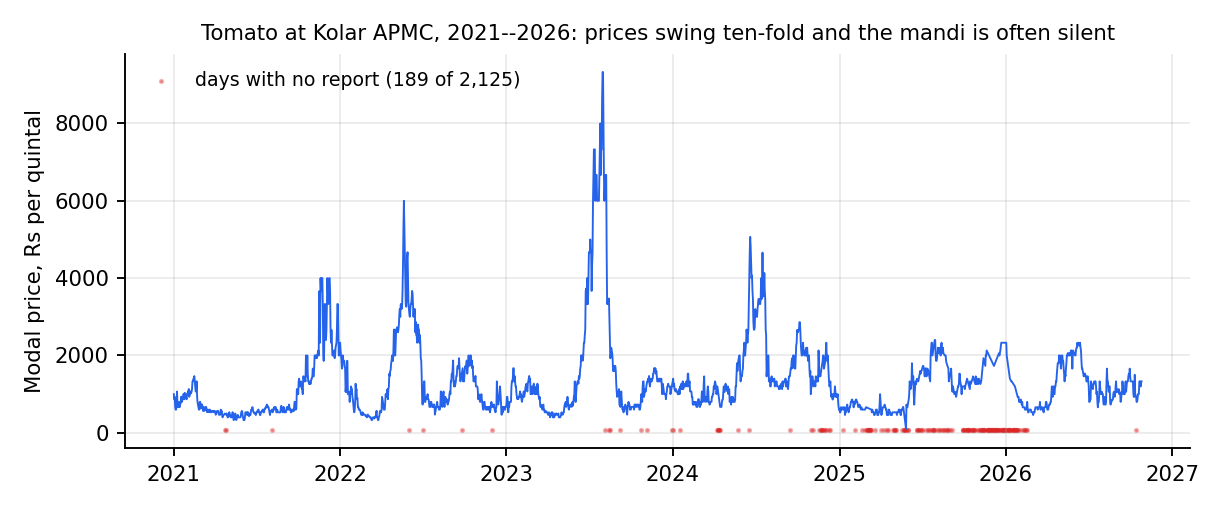
\includegraphics[width=0.95\textwidth]{figures/fig_intro_kolar_tomato.png}
    \caption{Modal price of tomato at Kolar APMC (Agmarknet, 2021--2026). The red marks along the bottom are days with no report; a farmer cannot tell from the portal whether such a day means no trade or no data.}
    \label{fig:kolar}
\end{figure}

Information matters to sellers. Field studies from southern India and West Africa found that when traders and fishermen could compare prices across markets by mobile phone, price dispersion fell and welfare rose~\cite{jensen2007,aker2010}. A price portal that lists yesterday's quotes is a weak form of that information. It gives a number for each market but not the answer to the farmer's question, which is \emph{where should this load go, and should it go today}.

Machine learning has been applied extensively to agricultural price forecasting, with hybrid models that decompose a price series and forecast the pieces reporting very large gains~\cite{ray2023,sathe2025,celik2025,wu2026}. This project took a different starting point. A forecast is useful only through the decision it supports, so the quantity to be judged is the money a farmer ends up with, and that has to be measured on data the model could not have seen.

Three further needs follow from how farmers and traders actually use such a tool. First, a number is not advice: a farmer who reads Kannada, or a trader short of time, wants a plain recommendation with reasons, and language models can write one, but they also invent figures, so any brief they write must be checked against the evidence before it is shown. Second, crops do not move alone. A shortage of tomato can pull on the price of onion or potato, and a trader holding several crops needs to know whether such links are real or are the common market movement seen through a different lens. Third, advice has to be inspectable and has to reach the farmer where they are: a farmer asks why a faraway mandi beats the nearest one, an examiner asks what happens if everyone follows the advice, and a recommendation that waits on a web page nobody opens helps no one. Chapters~\ref{ch:method}--\ref{ch:results} treat all three needs with the same discipline as the main engine: claims are tested on held-out data and withheld when the evidence does not support them.

\section{Objectives}
\label{sec:objectives}

\noindent \textbf{Primary objective.} To build and evaluate a decision-support system that recommends, for a farmer's crop and location, the mandi and the holding period that maximise net revenue, and that states a revenue floor the recommendation is verified to respect.

\noindent \textbf{Specific objectives.}
\begin{enumerate}
    \item To construct, by 31 October 2026, a clean panel from the real Agmarknet history for the Bengaluru--Kolar belt (at least 30,000 mandi-days, four crops) with every cleaning step and exclusion recorded.
    \item To formulate net revenue per quintal from price, shrinkage, transport cost and the probability that a market is silent, and to train a market-choice model on it, measuring regret against a hindsight oracle on at least 500 held-out days per crop.
    \item To test, with block-bootstrap intervals and Holm-corrected paired tests, whether (a) realised-revenue labels and (b) a decision-focused loss improve on conventional training, and to report the result whether or not it is favourable.
    \item To derive revenue floors whose empirical violation rate is within two percentage points of the nominal level at 10\% over a walk-forward evaluation.
    \item To deliver the engine through a FastAPI service and a trilingual (English, Kannada, Hindi) web application for farmers and traders, with automated tests and a reproducible pipeline from raw data to served model.
    \item To audit published decompose-then-forecast price models for look-ahead leakage and to benchmark against a zero-shot foundation model.
    \item To build an LLM-based \emph{decision intelligence} service that turns the engine's evidence into a structured brief (action BUY, SELL, HOLD or WAIT, a confidence level, and factors that each cite their evidence), and to verify every figure in a brief against the evidence it was given, with a deterministic fallback when the model fails or its answer is not grounded. Success is measured by the share of explanation sentences kept after an independent faithfulness judge in English, Kannada and Hindi, and by the judge catching at least eight of nine deliberately corrupted explanations without rejecting faithful ones.
    \item To estimate \emph{cross-commodity spillover}, that is, how a supply shock in one of five crops transmits to the prices of the others after removing the common market factor and seasonality, for all 40 ordered source--target--direction combinations, with episode-level bootstrap intervals and false-discovery-rate control, publishing an edge only when at least eight shock episodes support it.
    \item To make the advice inspectable and auditable with five features built on the engine: a per-quintal breakdown whose parts add up to the served net revenue (within Rs~1); a what-if simulator that re-prices the advice under the farmer's own costs and reports the cost at which it changes; a day-by-day track record on days the advice was not fitted on, whose headline numbers reproduce the back-test; a silence tax per mandi; and a crowd simulator for many farmers following the same advice, with every scenario parameter stated.
    \item To deliver a dated morning digest in English, Kannada and Hindi through a free messaging channel (Telegram) built only from ingested data, giving selling advice only for crops whose evidence is strong, and to demonstrate it end to end with a delivery log. A field pilot with farmers is outside this objective.
\end{enumerate}

\section{Problem Statement}
\label{sec:problem-statement}

A seller of a perishable crop faces a joint choice of destination $m\in\mathcal{M}$ and holding days $k\in\{0,1,2,3\}$, or sale at the farm gate. Define the net revenue per quintal of action $(m,k)$ on day $t$ as the price realised at $m$ on day $t+k$, less the value lost to shrinkage, less transport cost, with a penalty when $m$ does not report. The farmer observes only past prices, and observes them only for markets and days that were reported. The problem is to choose an action that maximises realised revenue and to state, before the sale, a floor below which revenue will fall only rarely.

Three properties make the problem harder than forecasting a price series. First, \emph{selective reporting}: the price at a market is missing on the days it is least informative to the model, and a model trained only on posted prices learns that every market is always open. Second, \emph{the object of interest is a decision}, so the error that matters is regret, the revenue lost relative to the best action in hindsight, not the squared error of a price. Third, \emph{a recommendation without an error statement is not usable}: a farmer who gambles a harvest needs to know how bad the outcome can be.

\noindent \textbf{Scope.} Four crops (tomato, onion, potato, ginger) in the Bengaluru--Kolar belt; daily modal prices; the Agmarknet source only; offline evaluation on history. Two supporting services are in scope: a grounded decision brief written by a language model over the engine's evidence, and an estimate of how supply shocks in one crop spill over to the others. Five insight features that explain and audit the advice, and a Telegram morning digest, are also in scope. Garlic was excluded from market choice because only one mandi had enough reported days, so no choice between markets exists. Field trials with farmers, price effects of the system's own advice, and live market access are outside the scope.

\section{Summary}
\label{sec:intro-summary}

The chapter argued that the farmer's question is a decision under uncertainty with missing data and that judging it by forecast error misses the point. The primary objective is a recommendation with a verified floor, supported by ten measurable objectives, the last four being a grounded language-model decision brief, a cross-commodity spillover estimate, five features that explain and audit the advice, and a morning digest on a free messaging channel. Chapter~\ref{ch:lit} reviews related work and the gaps this project fills. Chapter~\ref{ch:method} sets out requirements, the proposed method, architecture, dataset and evaluation design. Chapter~\ref{ch:plan} documents planning and management. Chapter~\ref{ch:impl} describes implementation, integration and testing. Chapter~\ref{ch:results} reports results, including those that did not work. Chapter~\ref{ch:concl} concludes with learnings, limitations, future work and the mapping to engineering outcomes and sustainable development goals. The appendices hold code, the survey instrument, evaluation tables, dataset description, outcome mapping and the similarity record.

\chapter{Literature Review}
\label{ch:lit}

This chapter reviews the work on which MandiSense AI rests and states, from that work, the problem the thesis addresses. The review has two parts. The first is a systematic survey, carried out in the initial stage of the project, of \textbf{25 recent studies} on agricultural price prediction, volatility and anomaly analysis, hybrid and ensemble forecasting, and smart-farming decision support (Section~\ref{sec:survey}); each study is compared on its techniques, results, research gaps and takeaways. The second widens the view to the methods the system uses (decision-focused learning, conformal prediction, missing data, forecast evaluation and language-model grounding) and to the economics of Indian agricultural markets. Every reference in the Bibliography was looked up by title and author in a public bibliographic index (Crossref or arXiv) before it was listed.

Section~\ref{sec:lit-markets} describes the setting and the evidence that information changes farmer outcomes. Sections~\ref{sec:related-forecast} to~\ref{sec:evaluation} cover forecasting, decomposition hybrids and evaluation. Section~\ref{sec:survey} presents the survey with comparison tables. Sections~\ref{sec:ml-decision} to~\ref{sec:llm} cover decisions, uncertainty, missing data, transmission and language models. Section~\ref{sec:limitations} gathers the gaps and Section~\ref{sec:problem} states the problem. Figure~\ref{fig:taxonomy} places the strands of work and the point at which this project joins them.

\begin{figure}[!b]
\centering
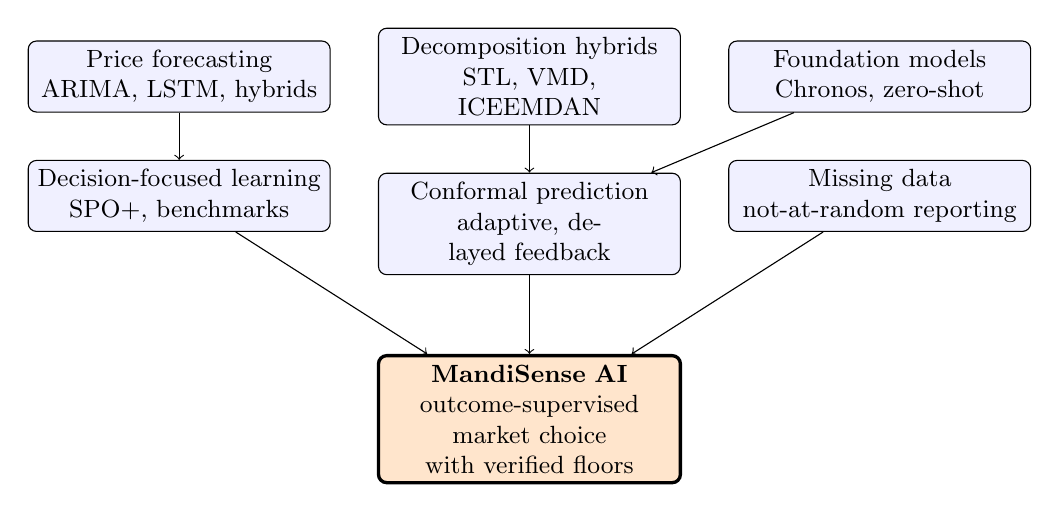
\begin{tikzpicture}[node distance=6mm, every node/.style={font=\small}, box/.style={draw, rounded corners=3pt, align=center, minimum height=9mm, text width=3.6cm, fill=blue!6}, hi/.style={box, fill=orange!20, very thick}]
\node[box] (a) {Price forecasting\\ ARIMA, LSTM, hybrids};
\node[box, right=of a] (b) {Decomposition hybrids\\ STL, VMD, ICEEMDAN};
\node[box, right=of b] (c) {Foundation models\\ Chronos, zero-shot};
\node[box, below=of a] (d) {Decision-focused learning\\ SPO+, benchmarks};
\node[box, below=of b] (e) {Conformal prediction\\ adaptive, delayed feedback};
\node[box, below=of c] (f) {Missing data\\ not-at-random reporting};
\node[hi, below=10mm of e] (g) {\textbf{MandiSense AI}\\ outcome-supervised market choice\\ with verified floors};
\draw[->] (a) -- (d); \draw[->] (b) -- (e); \draw[->] (c) -- (e); \draw[->] (f) -- (g); \draw[->] (d) -- (g); \draw[->] (e) -- (g);
\end{tikzpicture}
\caption{Strands of related work and where this project joins them.}
\label{fig:taxonomy}
\end{figure}

\section{Agricultural Markets and the Value of Information}
\label{sec:lit-markets}

Fruit and vegetable prices in India are volatile, and the volatility is not only a matter of weather: a study of onion prices traces large swings to supply shocks interacting with storage, trade policy and market structure~\cite{birthal2019}. The government publishes daily mandi quotations through AGMARKNET~\cite{agmarknet}, but a quotation is the price at one market on one day, not advice on where to sell.

The effect of price information on producers has been studied in several countries. In the South Indian fisheries sector, the arrival of mobile phones reduced price dispersion and raised both producer profit and consumer surplus~\cite{jensen2007}. In Niger, phones reduced search costs and price dispersion across grain markets~\cite{aker2010}. For Indian agriculture, a randomised study of text-message price information found that it changed some marketing decisions but had a limited average effect~\cite{fafchamps2012}.

\paragraph{What this means for the project.} The studies agree that a price quotation helps when it changes where or when a farmer sells, and that the effect is small when the information is generic or late. MandiSense AI therefore delivers a specific choice, in the farmer's language, with the date of every price shown (Chapter~\ref{ch:impl}), and not a price board. We do not claim any welfare effect: that would need a field trial, which is listed as future work (Chapter~\ref{ch:concl}).

\section{Related Work on Agricultural Price Forecasting}
\label{sec:related-forecast}

\subsection*{Statistical and neural forecasters}
Forecasting texts treat the random walk and seasonal methods as the benchmarks any new model must beat~\cite{hyndman2021}. Early work on Indian crops used time-delay neural networks for monthly wholesale prices of oilseeds~\cite{jha2014}. Later studies combined linear and recurrent models, for example an ARIMA--LSTM hybrid with random-forest feature selection for volatile series~\cite{ray2023}; applied deep models to ragi prices in Karnataka~\cite{meena2024}; guided networks with hidden Markov regimes for highly volatile commodities~\cite{avinash2024}; and, for multi-commodity settings, coupled attention models with anomaly detection~\cite{sediyono2025}. A modular machine-learning framework predicts crop yield, supply and demand before the price~\cite{mohanty2023}, and deep models with exogenous drivers such as weather and supply factors improved forecasts of tomato, onion and potato prices~\cite{exogenous2024}. A recent review catalogues this architectural variety and flags open challenges~\cite{wu2026}. Work on farmers' choices shows that crop insurance affects diversification, which links price information to planting decisions~\cite{crop_ins}.

\subsection*{Volatility}
Volatility is the quantity a farmer feels as risk. A hybrid LSTM--GARCH model, applied to 23 commodities across 165 Indian markets, captured both non-linear dynamics and volatility clustering and gave lower error than standalone econometric and deep models~\cite{manogna2025}. This is the model family behind the volatility view of the trader desk (Chapter~\ref{ch:impl}).

\subsection*{Gradient boosting and foundation models}
Gradient-boosted trees~\cite{chen2016,ke2017} remain strong on tabular data, where they often outperform deep networks~\cite{grinsztajn2022}. Pretrained time-series foundation models forecast new series without training~\cite{ansari2024}, and early evidence for commodity prices is cautiously positive~\cite{wang2026}. Both belong in a fair benchmark, so both are included in Chapter~\ref{ch:results}.

\section{Decomposition Hybrids and the Leakage Problem}
\label{sec:hybrids}

A large strand of work splits the price into components and forecasts each part. The classical decomposition is STL, which separates trend, seasonal and remainder by loess~\cite{cleveland1990}; variational mode decomposition extracts intrinsic modes by constrained optimisation~\cite{dragomiretskiy2014}. Reported gains are large: an STL--LSTM hybrid for seasonal series~\cite{jaiswal2025}, CEEMDAN-based hybrids for non-linear prices~\cite{ceemdan2024}, ICEEMDAN--VMD--GRU~\cite{sathe2025}, ensembles of machine-learning, time-series and stochastic models~\cite{celik2025}, and a decomposition-ensemble with kernel density estimation for point and interval forecasts~\cite{kde2024}.

The concern with this design is that a decomposition computed on the whole series before the split lets future values shape the components used to predict them. The evaluation literature warns about time-ordered validation in general~\cite{bergmeir2012,cerqueira2020}, but we found no agricultural study that measured the size of the leak. Section~\ref{sec:leakage} does.

\section{Evaluation and Statistical Comparison}
\label{sec:evaluation}

Predictive accuracy is compared pairwise with the Diebold--Mariano test~\cite{diebold1995}, with a small-sample correction~\cite{harvey1997} and autocorrelation-robust variance~\cite{newey1987}. When many comparisons are made, familywise error is controlled by Holm's procedure~\cite{holm1979}, and a model confidence set identifies the models that cannot be separated from the best~\cite{hansen2011}. Dependence in the data is respected by resampling blocks rather than days~\cite{kunsch1989}. Hyper-parameters are tuned inside the training window by Bayesian optimisation~\cite{akiba2019}, and the test period is touched once.

\section{Systematic Survey of 25 Studies (2023--2025)}
\label{sec:survey}

\subsection{Survey protocol}
The survey was carried out in the initial stage of the project and recorded in a shared workbook with the same fields for every paper: title, publication, abstract, techniques, results, year, link, research gaps and key takeaways. The work was divided among the three team members. The search was limited to peer-reviewed journal and conference papers from 2023 to 2025 on agricultural price prediction, volatility and anomaly analysis, hybrid and ensemble forecasting, and smart-farming decision support, drawn from Springer Nature, Elsevier ScienceDirect and IEEE Xplore. After removing duplicates (six IEEE papers were recorded by two members), \textbf{25 distinct studies} remained, labelled S1 to S25. Every study was matched to a bibliographic record in Crossref before it was cited. The findings below are the authors' own, as recorded in the workbook from the abstracts and results sections; performance figures were not re-measured by us.

\begin{table}[!t]
\centering
\caption{Distribution of the 25 surveyed studies by publisher and year (as recorded in the workbook)}
\label{tab:survey-dist}
\small
\begin{tabular}{|l|c|c|c|c|}
\hline
\textbf{Source} & \textbf{2023} & \textbf{2024} & \textbf{2025} & \textbf{Total} \\ \hline
Elsevier (ScienceDirect), S1--S10 & 2 & 5 & 3 & 10 \\ \hline
Springer Nature, S11--S19 & 2 & 5 & 2 & 9 \\ \hline
IEEE, S20--S25 & 1 & 3 & 2 & 6 \\ \hline
\textbf{Total} & \textbf{5} & \textbf{13} & \textbf{7} & \textbf{25} \\ \hline
\end{tabular}
\end{table}

\subsection{Overview of the studies}
Table~\ref{tab:survey-overview} lists the studies with their venue and the task they address. Of the 25, 15 forecast prices (S2 also detects anomalies), 5 concern volatility or its drivers, 1 is about anomaly detection, and 4 are crop-recommendation systems or reviews.

\Needspace{12\baselineskip}
{\footnotesize\setlength{\tabcolsep}{4pt}\renewcommand{\arraystretch}{1.15}
\begin{longtable}{|p{0.9cm}|p{7.7cm}|p{4.2cm}|p{2.7cm}|}
\caption{The 25 surveyed studies}\label{tab:survey-overview}\\
\hline \textbf{ID} & \textbf{Study} & \textbf{Venue} & \textbf{Task} \\ \hline \endfirsthead
\hline \textbf{ID} & \textbf{Study} & \textbf{Venue} & \textbf{Task} \\ \hline \endhead
\hline \endfoot
S1 & Hybrid forecasting of commodity prices: machine learning, time series and stochastic simulation~\cite{celik2025} & Borsa \.Istanbul Rev., 2025 & Price, risk \\ \hline
S2 & Multi-commodity price forecasting and anomaly detection with attention-boosted models~\cite{sediyono2025} & J. Agric. Food Res., 2025 & Price, anomaly \\ \hline
S3 & ARIMA--LSTM for volatile prices with random forest~\cite{ray2023} & Appl. Soft Comput., 2023 & Price \\ \hline
S4 & ICEEMDAN--VMD--GRU for economic resilience~\cite{sathe2025} & Results Eng., 2025 & Price \\ \hline
S5 & Volatility dynamics of agricultural futures under uncertainties~\cite{fiszeder2024} & Energy Econ., 2024 & Volatility \\ \hline
S6 & Financial stress and realised volatility of agricultural commodities~\cite{algirdas2024} & Res. Int. Bus. Finance, 2024 & Volatility \\ \hline
S7 & Optimal forecast combination (PSO-CS) for daily futures prices~\cite{zeng2023} & Appl. Soft Comput., 2023 & Price, ensemble \\ \hline
S8 & Transformer anomaly detection with inter-variable attention~\cite{tranad2024} & Inf. Fusion, 2024 & Anomaly \\ \hline
S9 & Hidden-Markov-guided deep models for volatile prices~\cite{avinash2024} & Appl. Soft Comput., 2024 & Price \\ \hline
S10 & Economic policy uncertainty and agricultural prices, China~\cite{epu2024} & Asia Global Econ., 2024 & Volatility \\ \hline
S11 & STL--LSTM for seasonal agricultural price series~\cite{jaiswal2025} & Ann. Data Sci., 2025 & Price \\ \hline
S12 & CEEMDAN hybrid models for agricultural prices~\cite{ceemdan2024} & Sci. Rep., 2024/25 & Price \\ \hline
S13 & Exogenous-variable deep learning for tomato, onion, potato~\cite{exogenous2024} & Sci. Rep., 2024 & Price \\ \hline
S14 & Hybrid LSTM--GARCH volatility forecasting, India~\cite{manogna2025} & J. Big Data, 2025 & Volatility \\ \hline
S15 & Commodity price prediction: a machine-learning framework~\cite{mohanty2023} & Neural Comput. Appl., 2023 & Price \\ \hline
S16 & Demand and price forecasting using deep learning~\cite{demand2023} & LNCS (MIWAI), 2023 & Price, demand \\ \hline
S17 & Point and interval forecasting, decomposition-ensemble and KDE~\cite{kde2024} & Soft Comput., 2024 & Price, interval \\ \hline
S18 & Optimised machine learning for commodity prices~\cite{optimized2023} & Neural Comput. Appl., 2024 & Price \\ \hline
S19 & GCN--BiGRU--TPE futures price prediction~\cite{gcn2024} & Comput. Econ., 2025 & Price, graph \\ \hline
S20 & Crop yield prediction and recommendation, deep ensembles (survey)~\cite{cropyield} & IEEE conf., 2024 & Crop, survey \\ \hline
S21 & Framework for ragi price prediction in Karnataka~\cite{meena2024} & IEEE Access, 2024 & Price \\ \hline
S22 & AgTech: volatility prediction for commodity trading~\cite{agtech2024} & IEEE Access, 2024 & Volatility \\ \hline
S23 & Smart agriculture: state, opportunities and challenges~\cite{smartag2024} & IEEE Access, 2024 & Review \\ \hline
S24 & Smart farming: crop recommendation and price prediction~\cite{smartfarm2025} & IEEE conf., 2025 & Crop, price \\ \hline
S25 & Federated explainable AI for smart agriculture~\cite{fedxai2025} & IEEE Access, 2025 & Crop, XAI \\ \hline
\end{longtable}}

\subsection{Techniques and results}
Tables~\ref{tab:survey-t1} to~\ref{tab:survey-t3} record, for each study, the techniques used and the principal results as reported by the authors.

\Needspace{12\baselineskip}
{\footnotesize\setlength{\tabcolsep}{4pt}\renewcommand{\arraystretch}{1.15}
\begin{longtable}{|p{0.9cm}|p{5.8cm}|p{9.2cm}|}
\caption{Techniques and results, S1--S10 (price, volatility and anomaly studies, Elsevier)}\label{tab:survey-t1}\\
\hline \textbf{ID} & \textbf{Techniques} & \textbf{Principal results} \\ \hline \endfirsthead
\hline \textbf{ID} & \textbf{Techniques} & \textbf{Principal results} \\ \hline \endhead
\hline \endfoot
S1 & ARIMA, VAR, LSTM and stochastic simulation (geometric, fractional and bridge Brownian motion); value-at-risk & LSTM best in high-volatility and crisis periods; ARIMA stable in short-term, low-volatility markets; geometric Brownian motion balances accuracy and risk; fractional motion captures long memory but raises volatility \\ \hline
S2 & Transformer forecasting; attention-boosted LSTM variational autoencoder for anomalies & Transformers beat LSTM and GRU in price forecasting; the attention-boosted autoencoder improves anomaly detection and captures sudden spikes and drops \\ \hline
S3 & ARIMA plus LSTM hybrid; random-forest selection of lags and features; volatility modelling & ARIMA captures linear trend, LSTM the non-linear part, random forest improves feature selection; the hybrid cuts RMSE and MAPE markedly \\ \hline
S4 & ICEEMDAN and VMD decomposition followed by GRU & Decomposition reduces noise and non-stationarity; the hybrid outperforms LSTM and RNN variants \\ \hline
S5 & Heterogeneous autoregressive (HAR) models, LASSO; news-based and market-based uncertainty indicators & Market-based indicators outperform news-based ones; LASSO improves on HAR; uncertainty is strongly linked to price volatility \\ \hline
S6 & HAR-RV variants on high-frequency realised volatility & Financial stress predicts realised volatility in-sample and shows financialisation of agricultural markets; out-of-sample prediction is inconsistent \\ \hline
S7 & EWT, SSA and VMD decomposition; ARIMA, ETS, BPNN, ELM; PSO-CS weight optimisation & The optimised ensemble beats all single models, with a large reduction in MAPE \\ \hline
S8 & Variable temporal transformer with self-attention for multivariate anomaly detection & Captures temporal and inter-variable dependence, beats traditional detectors and gives interpretable anomaly explanations \\ \hline
S9 & Hidden Markov model with RNN, LSTM, GRU, BiLSTM, CNN; technical indicators and FFT & The Markov model captures regime change; guided deep models beat the same models alone for short and medium horizons \\ \hline
S10 & Time-varying-parameter VAR for transmission of policy uncertainty & Policy uncertainty affects price volatility, with effects that vary over time and across commodities \\ \hline
\end{longtable}}

\Needspace{12\baselineskip}
{\footnotesize\setlength{\tabcolsep}{4pt}\renewcommand{\arraystretch}{1.15}
\begin{longtable}{|p{0.9cm}|p{5.8cm}|p{9.2cm}|}
\caption{Techniques and results, S11--S19 (Springer Nature)}\label{tab:survey-t2}\\
\hline \textbf{ID} & \textbf{Techniques} & \textbf{Principal results} \\ \hline \endfirsthead
\hline \textbf{ID} & \textbf{Techniques} & \textbf{Principal results} \\ \hline \endhead
\hline \endfoot
S11 & STL decomposition into trend, seasonal and remainder; an LSTM per component; recombined forecast & Beat ARIMA and a plain LSTM; seasonal components predicted more reliably; RMSE and MAPE improved on benchmarks \\ \hline
S12 & CEEMDAN decomposition with a time-delay neural network per component; compared with ARIMA, random forest, GBM, SVR & Best of all models; RMSE about 20\% lower than other EMD-based models and about 57\% lower than traditional machine learning; MAPE near 2--4\% for major crops \\ \hline
S13 & NBEATSX and TransformerX with weather variables; compared with ARIMAX, ANN, SVR, random forest, XGBoost; RMSE, MAE, sMAPE, MASE & NBEATSX best for all three crops (tomato, onion, potato); deep models clearly beat statistical and machine-learning baselines \\ \hline
S14 & LSTM for long-term pattern; GARCH on LSTM residuals; compared with GARCH, GJR-GARCH, EWMA, MEM & Best for all commodities; onion RMSE fell from 5.44 (GARCH) to 0.70, tomato from 7.67 to 0.79 \\ \hline
S15 & ARIMA, AR, MA, ES, STL for yield; supply from yield, residue and imports; demand by time series; decision tree, RF, KNN, kernel ridge for price & ARIMA(4,1,1) best for yield; decision-tree regressor best for price (RMSE about 0.115, MAPE about 14\%) \\ \hline
S16 & RNN, LSTM and bidirectional LSTM compared with statistical and machine-learning methods; horizon up to one year & LSTM and Bi-LSTM capture temporal dependence better than ARIMA variants; detailed error figures are not available in the accessible preview \\ \hline
S17 & VMD with energy entropy; K-means reconstruction; ARIMA for low and LSTM for high frequencies; WOA-optimised adaptive KDE intervals & Lowest error among compared methods; MAPE about 1--2\% one step ahead; interval coverage (PICP) above 95\% at the 95\% level; 5--15\% lower RMSE than other hybrids \\ \hline
S18 & Extreme learning machine and LSTM tuned by genetic algorithm; Auto-ARIMA; 11 commodities, daily 2000--2022 & GA-ELM best overall (MAPE about 1--3\%), trains faster than GA-LSTM, forecasts 60 days ahead and follows the 2022 peaks \\ \hline
S19 & Multi-graph construction; graph convolution for spatial structure; BiGRU for time; TPE Bayesian tuning & On corn futures, RMSE about 20.2, MAPE about 0.55\%, $R^2$ about 0.97 \\ \hline
\end{longtable}}

\Needspace{12\baselineskip}
{\footnotesize\setlength{\tabcolsep}{4pt}\renewcommand{\arraystretch}{1.15}
\begin{longtable}{|p{0.9cm}|p{5.8cm}|p{9.2cm}|}
\caption{Techniques and results, S20--S25 (IEEE)}\label{tab:survey-t3}\\
\hline \textbf{ID} & \textbf{Techniques} & \textbf{Principal results} \\ \hline \endfirsthead
\hline \textbf{ID} & \textbf{Techniques} & \textbf{Principal results} \\ \hline \endhead
\hline \endfoot
S20 & PSO and WOA for feature selection; SVM, random forest, RNN, Bi-LSTM, CNN, MLP and ensembles (survey of methods) & Ensemble and optimisation approaches outperform traditional methods in crop prediction; Bi-LSTM and CNN strongest on climate and crop data \\ \hline
S21 & LSTM deep-learning framework with temporal and seasonal features; compared with statistical and machine-learning models & Higher accuracy on ragi price trends, robust to non-linear fluctuations, better precision and recall than baselines \\ \hline
S22 & Bi-LSTM on multivariate market indicators (price, volume, open interest); rolling-window volatility index; dropout; binary classification of high/low volatility & Improved accuracy of volatility forecasts for exchange-traded commodities; robust to sudden fluctuations; fewer false predictions \\ \hline
S23 & Survey of IoT, AI and machine learning, blockchain, cloud and precision farming & Documents gains in resource efficiency (water, fertiliser, energy) and applications in precision farming, monitoring and yield prediction \\ \hline
S24 & XGBoost, random forest, decision tree, SVM, KNN, naive Bayes, linear and logistic regression & Integrated crop recommendation and price prediction; ensembles most accurate; price models more reliable than traditional statistics \\ \hline
S25 & Federated learning with explainable AI; CNN, LSTM, RF, SVM, gradient boosting; SHAP and LIME & Better crop-recommendation accuracy across distributed data while preserving privacy; transparent predictions; scales across regions \\ \hline
\end{longtable}}

\subsection{Research gaps and takeaways}
Tables~\ref{tab:survey-g1} to~\ref{tab:survey-g3} record the gaps named for each study in the workbook and the lesson each gives for MandiSense AI.

\Needspace{12\baselineskip}
{\footnotesize\setlength{\tabcolsep}{4pt}\renewcommand{\arraystretch}{1.15}
\begin{longtable}{|p{0.9cm}|p{6.4cm}|p{8.6cm}|}
\caption{Research gaps and takeaways, S1--S10}\label{tab:survey-g1}\\
\hline \textbf{ID} & \textbf{Research gaps} & \textbf{Takeaways for this project} \\ \hline \endfirsthead
\hline \textbf{ID} & \textbf{Research gaps} & \textbf{Takeaways for this project} \\ \hline \endhead
\hline \endfoot
S1 & Models used independently; no shock detection; volatility not in decision support; no explainable architecture & No single model wins in every regime, so a council of specialists is justified; risk-aware, adaptive systems are needed \\ \hline
S2 & Centralised, not agent-based; no explicit risk quantification; limited decision-support integration & Joint forecasting and anomaly detection works; risk and explanation still need to be added \\ \hline
S3 & Monthly data only; no ensemble extension; volatility handled indirectly & Hybrid statistical-plus-deep models beat single models; feature selection matters \\ \hline
S4 & High computational cost; no volatility or anomaly module; one pipeline & Noise reduction is critical for agricultural series; decomposition plus deep learning is effective (and, here, audited for leakage) \\ \hline
S5 & Volatility only, not price; not linked to forecasting or decisions & External uncertainty signals matter; volatility should be tied to price prediction \\ \hline
S6 & Out-of-sample reliability weak; not linked to price models & Financial stress is a volatility driver; regimes change; adaptive models are needed \\ \hline
S7 & Centralised; no explainability or volatility alerts; costly & Combination improves accuracy and stability; weight optimisation is crucial \\ \hline
S8 & Not integrated with price forecasting; little agricultural use; intensive & Attention helps anomaly detection; anomaly detection should be coupled with forecasting \\ \hline
S9 & Commodity- and region-specific; no ensemble or multi-agent design; limited explainability & Regime awareness improves forecasts; probabilistic-plus-deep hybrids suit volatile series \\ \hline
S10 & China only; no forecasting framework & Policy uncertainty drives volatility; time-varying models are needed; policy effects belong in forecasting systems \\ \hline
\end{longtable}}

\Needspace{12\baselineskip}
{\footnotesize\setlength{\tabcolsep}{4pt}\renewcommand{\arraystretch}{1.15}
\begin{longtable}{|p{0.9cm}|p{6.4cm}|p{8.6cm}|}
\caption{Research gaps and takeaways, S11--S19}\label{tab:survey-g2}\\
\hline \textbf{ID} & \textbf{Research gaps} & \textbf{Takeaways for this project} \\ \hline \endfirsthead
\hline \textbf{ID} & \textbf{Research gaps} & \textbf{Takeaways for this project} \\ \hline \endhead
\hline \endfoot
S11 & Weather, supply and demand shocks and market events not used; centralised & Decomposition handles strong seasonality, as in mandi series; preprocessing to isolate components helps deep models \\ \hline
S12 & History only, no weather or demand; centralised & Decomposition before prediction helps volatile prices; hybrids are more reliable than single models \\ \hline
S13 & Only weather; no demand, festivals or exports; centralised & External factors improve accuracy; multi-input forecasting suits Indian markets \\ \hline
S14 & Price history only; centralised & LSTM--GARCH suits abnormal-volatility detection and risk alerts; volatility should join multi-model forecasting \\ \hline
S15 & One crop (corn); no deep learning or real-time data & Integrating supply and demand improves price forecasts; multi-factor beats price alone \\ \hline
S16 & Few metrics reported; no exogenous drivers & Deep sequence models capture temporal trend; test several architectures; report detailed errors \\ \hline
S17 & Price history only; computationally complex & Intervals support risk-aware decisions; ARIMA plus LSTM improves stability; ranges should accompany forecasts \\ \hline
S18 & No external factors; centralised & Optimised hybrids are stable; 60-day forecasts are feasible; compare several models; add arrivals, season and festivals \\ \hline
S19 & One commodity; no weather or demand cycles & Graph structure suits mandis linked by trade; Bayesian tuning automates configuration \\ \hline
\end{longtable}}

\Needspace{12\baselineskip}
{\footnotesize\setlength{\tabcolsep}{4pt}\renewcommand{\arraystretch}{1.15}
\begin{longtable}{|p{0.9cm}|p{6.4cm}|p{8.6cm}|}
\caption{Research gaps and takeaways, S20--S25}\label{tab:survey-g3}\\
\hline \textbf{ID} & \textbf{Research gaps} & \textbf{Takeaways for this project} \\ \hline \endfirsthead
\hline \textbf{ID} & \textbf{Research gaps} & \textbf{Takeaways for this project} \\ \hline \endhead
\hline \endfoot
S20 & Few multi-source datasets; no standard feature engineering; narrow metrics; little interpretability & Ensembles and optimisation help; precision, recall and F1 should be reported; false rates affect trust \\ \hline
S21 & One crop; no socio-economic factors; no deployment study; interpretability & LSTM models suit price series; temporal features help; the framework supports farmers and policymakers \\ \hline
S22 & Policy factors missing; no deployment or multi-commodity scale; interpretability; cross-market links & Volatility prediction can steady trading decisions; ensembles beat single models; external features help \\ \hline
S23 & Little real-time deployment in developing regions; interoperability; privacy; farmer usability & Smart agriculture reduces waste and raises productivity; adoption depends on farmers; solutions must suit smallholders \\ \hline
S24 & No real-time integrated deployment; socio-economic and policy factors; interpretability; scalability & Crop recommendation and price forecasting together support market decisions; multi-source data is crucial \\ \hline
S25 & No real-time rural deployment; interoperability; efficiency against explainability; farmer usability; security & Federated learning avoids sharing raw farmer data; explanations build trust \\ \hline
\end{longtable}}

\subsection{Comparison matrix}
Table~\ref{tab:survey-matrix} compares the studies on ten properties. A tick means the study uses or addresses the property. The last row shows MandiSense AI for reference.

\begin{table}[!t]
\centering
\caption{Comparison of the surveyed studies on ten properties}
\label{tab:survey-matrix}
\footnotesize
\setlength{\tabcolsep}{4.6pt}
\renewcommand{\arraystretch}{1.1}
\begin{tabular}{|l|c|c|c|c|c|c|c|c|c|c|}
\hline
\textbf{ID} & \textbf{Decomp.} & \textbf{RNN} & \textbf{Attn.} & \textbf{Volat.} & \textbf{Ensemble} & \textbf{Exog.} & \textbf{Interval} & \textbf{Anomaly} & \textbf{Graph} & \textbf{Decision} \\ \hline
S1  & & $\checkmark$ & & $\checkmark$ & $\checkmark$ & & & & & \\ \hline
S2  & & & $\checkmark$ & & & & & $\checkmark$ & & \\ \hline
S3  & & $\checkmark$ & & $\checkmark$ & $\checkmark$ & & & & & \\ \hline
S4  & $\checkmark$ & $\checkmark$ & & & & & & & & \\ \hline
S5  & & & & $\checkmark$ & & $\checkmark$ & & & & \\ \hline
S6  & & & & $\checkmark$ & & $\checkmark$ & & & & \\ \hline
S7  & $\checkmark$ & & & & $\checkmark$ & & & & & \\ \hline
S8  & & & $\checkmark$ & & & & & $\checkmark$ & & \\ \hline
S9  & & $\checkmark$ & & $\checkmark$ & & & & & & \\ \hline
S10 & & & & $\checkmark$ & & $\checkmark$ & & & & \\ \hline
S11 & $\checkmark$ & $\checkmark$ & & & & & & & & \\ \hline
S12 & $\checkmark$ & & & & & & & & & \\ \hline
S13 & & & $\checkmark$ & & & $\checkmark$ & & & & \\ \hline
S14 & & $\checkmark$ & & $\checkmark$ & & & & & & \\ \hline
S15 & & & & & & $\checkmark$ & & & & \\ \hline
S16 & & $\checkmark$ & & & & & & & & \\ \hline
S17 & $\checkmark$ & $\checkmark$ & & & $\checkmark$ & & $\checkmark$ & & & \\ \hline
S18 & & $\checkmark$ & & & $\checkmark$ & & & & & \\ \hline
S19 & & $\checkmark$ & & & & & & & $\checkmark$ & \\ \hline
S20 & & $\checkmark$ & & & $\checkmark$ & $\checkmark$ & & & & $\checkmark$ \\ \hline
S21 & & $\checkmark$ & & & & & & & & \\ \hline
S22 & & $\checkmark$ & & $\checkmark$ & & $\checkmark$ & & & & \\ \hline
S23 & & & & & & & & & & \\ \hline
S24 & & & & & $\checkmark$ & $\checkmark$ & & & & $\checkmark$ \\ \hline
S25 & & $\checkmark$ & & & & & & & & $\checkmark$ \\ \hline
\textbf{Total} & \textbf{5} & \textbf{14} & \textbf{3} & \textbf{8} & \textbf{7} & \textbf{8} & \textbf{1} & \textbf{2} & \textbf{1} & \textbf{3} \\ \hline
\textbf{This work} & $\checkmark$ & & $\checkmark$ & $\checkmark$ & $\checkmark$ & & $\checkmark$ & $\checkmark$ & $\checkmark$ & $\checkmark$ \\ \hline
\end{tabular}
\par\smallskip{\footnotesize Decomp.: decomposition; Attn.: attention or transformer; Volat.: volatility or risk modelling; Exog.: external drivers; Interval: prediction intervals; Graph: spatial or graph structure; Decision: output tied to a farmer decision. \emph{This work}: leakage audit of decomposition, zero-shot transformer baseline, volatility desk, council, conformal floors, shock desk, spillover engine, market choice.}
\end{table}

\subsection{Gap analysis across the survey}
The gaps recorded for the 25 studies fall into a small number of themes. Table~\ref{tab:survey-gaps} counts how many studies name each and states how the present work responds.

\begin{table}[!t]
\centering
\caption{Recurring gaps in the surveyed studies and the response of this project}
\label{tab:survey-gaps}
\small
\renewcommand{\arraystretch}{1.15}
\begin{tabular}{|p{4.0cm}|p{3.4cm}|c|p{6.4cm}|}
\hline
\textbf{Gap theme} & \textbf{Studies} & \textbf{n} & \textbf{Response in MandiSense AI} \\ \hline
External drivers (weather, demand, policy, socio-economic) not used & S11--S19, S21, S22, S24 & 12 & Arrivals, season and calendar features in the panel; a decision-focused label; no weather feed (live data not available) \\ \hline
Centralised design, no multi-agent or distributed structure & S2, S3, S7, S9, S11, S12, S14, S18 & 8 & Specialist council with learned weights and per-crop engines behind one API (Section~\ref{sec:architecture}) \\ \hline
Weak interpretability or explainability & S1, S7, S9, S20--S22, S24, S25 & 8 & Why-this-mandi breakdown, what-if, track record and a checked brief (Section~\ref{sec:insight-method}) \\ \hline
No real-time deployment or scalability study & S5, S6, S10, S21--S25 & 8 & A running service, a 60-check smoke test and a morning digest; no field trial yet \\ \hline
Volatility, risk or anomaly not tied to price or decisions & S1, S2, S4, S5, S6, S8, S10 & 7 & Shock desk, volatility view and revenue floors in the same service as the advice \\ \hline
Narrow data (one crop, market or region; monthly only) & S3, S9, S10, S15, S19, S21 & 6 & Four crops, 12 markets, daily data; one region (stated as a limit) \\ \hline
High computational cost & S4, S7, S8, S17 & 4 & Gradient boosting served; heavy models used only as challengers \\ \hline
Judged by forecast error, not by a decision & S1--S4, S7, S9, S11--S19, S21 & 16 & Regret and floor violation as the primary measures (Chapter~\ref{ch:results}) \\ \hline
Decomposition leakage not audited (our reading) & S4, S7, S11, S12, S17 & 5 & Walk-forward re-decomposition audit (Section~\ref{sec:leakage}) \\ \hline
\end{tabular}
\end{table}

Three conclusions follow. First, hybrid and decomposition-based models dominate recent work (14 of 25 use recurrent networks, 5 use decomposition) and are judged almost entirely by forecast error. Second, only one study (S17) provides an interval and none states a guarantee or a downside in rupees. Third, no study treats the farmer's own choice, of market and day, as the quantity to be optimised, and no study audits how much of the reported gain comes from fitting a decomposition on the whole series. These are the gaps that Section~\ref{sec:limitations} turns into objectives.


\section{Decisions, Not Forecasts}
\label{sec:ml-decision}

When forecasts feed an optimisation, minimising forecast error is not the same as minimising decision loss. The smart ``predict, then optimise'' (SPO+) loss trains a model directly on the regret of the decision it induces~\cite{elmachtoub2022}, and a recent benchmark across many decision-focused methods found the benefit to depend heavily on the problem~\cite{mandi2024}. For market choice the question is open, and Section~\ref{sec:effects} answers it for this problem. The neural variant used here encodes the set of markets with a permutation-invariant network~\cite{zaheer2017}, and a robust loss limits the influence of outlying prices on training~\cite{huber1964}.

\section{Calibrated Uncertainty}
\label{sec:uncertainty}

Conformal prediction gives intervals with finite-sample coverage under exchangeability~\cite{vovk2005,angelopoulos2023}, and conformalised quantile regression adapts the width to the input~\cite{romano2019}. Prices drift, so exchangeability fails; adaptive conformal inference tracks a long-run miscoverage rate under shift~\cite{gibbs2021}. A further complication, that the outcome of a sale is observed only days later, is handled in Section~\ref{sec:floors}.

\section{Missing and Informatively Missing Data}
\label{sec:missing}

A price is observed only when a market reports. If reporting depends on conditions the model also cares about, the data are not missing at random~\cite{rubin1976}, and learning from observed values alone is biased. Neural models for multivariate series with missing values add the missingness pattern itself as an input~\cite{che2018}; the same idea appears here as a reporting head and as silence features (Section~\ref{sec:formulation}).

\section{Transmission Between Commodities and the Effect of Followers}
\label{sec:transmission}

Prices of crops that share land, labour, storage or consumers move together, and some of that movement is the common market factor and the common season rather than transmission from one crop to another. Studies of transmission typically estimate it from whole series, which blends the three. The method used here removes the first common factor and each crop's calendar-month mean, defines shock episodes, and compares the response after an episode with the unconditional baseline, resampling over episodes rather than days (Section~\ref{sec:spill-method}) because days within an episode are strongly dependent~\cite{kunsch1989}; many pairs are tested, so multiplicity is controlled~\cite{holm1979}. Where the evidence is thin, the system withholds the claim.

A recommendation served to many users also changes what it predicts: a mandi that receives more produce than usual pays less, so advice that is good for one farmer can be poor for a thousand. This thesis treats that effect as a simulation with a stated price flexibility, not as a measured law (Section~\ref{sec:insight-method}). We did not find prior work that evaluates it for mandi choice, and cite none.

\section{Language Models for Explanation}
\label{sec:llm}

Language models can turn model output into readable advice in several languages, and tool-calling interfaces let a model fill a fixed schema instead of writing free text. The risk is that the text is fluent whether or not it is faithful: a model asked about prices will produce prices, some plausible and wrong. Work on foundation models for agricultural forecasting concerns the forecast itself~\cite{ansari2024,wang2026}; among the studies surveyed we found none that couples a language model to a price decision with a check that every stated figure appears in the evidence. This project treats the language model as a writer whose output is verified and may be discarded (Section~\ref{sec:intel-method}). The writer is an open-weight mixture-of-experts model~\cite{gptoss2025} and the judge is a different model family~\cite{qwen3}, so that the writer does not grade itself. Anthropic's Claude~\cite{claude3} was used by the authors as a development and writing assistant; Section~\ref{sec:ai-disclosure} describes that use.

\section{Limitations of Existing Systems}
\label{sec:limitations}

Table~\ref{tab:gaps} lists the limitations found and how each is addressed here. The first eight are properties of the literature; the last two are properties of what farmers actually have today: a price portal without advice, and no message that reaches them.

\begin{table}[!t]
    \centering
    \caption{Gaps in existing approaches and the objective that addresses each}
    \label{tab:gaps}
    \small
    \begin{tabular}{|p{4.6cm}|p{6.6cm}|p{3cm}|}
    \hline
    \textbf{Limitation} & \textbf{Description and impact} & \textbf{Addressed by} \\ \hline
    Judged on forecast error & Models are ranked by RMSE or MAPE; a model can win on error and still pick the wrong market~\cite{elmachtoub2022,mandi2024} & Objectives 2, 3 (Sec.~\ref{sec:effects}) \\ \hline
    Reporting gaps ignored & Training on posted prices only teaches the model that every market is open~\cite{rubin1976,che2018} & Objective 2 (Sec.~\ref{sec:formulation}) \\ \hline
    No statement of downside & Point forecasts, and intervals without guarantees, give a farmer nothing firm to set against the cost of a bad sale~\cite{kde2024,gibbs2021} & Objective 4 (Sec.~\ref{sec:floors}) \\ \hline
    Leakage in hybrid evaluation & Decompositions fitted on the full series flatter the reported skill~\cite{jaiswal2025,sathe2025,bergmeir2012} & Objective 6 (Sec.~\ref{sec:leakage}) \\ \hline
    Language-model advice is unchecked & A model can state a price that is nowhere in the evidence, and nothing in the text shows it & Objective 7 (Sec.~\ref{sec:intel-method}) \\ \hline
    Cross-crop effects confounded & Common movement and season look like transmission when estimated on whole series & Objective 8 (Sec.~\ref{sec:spill-method}) \\ \hline
    Advice cannot be inspected & A recommendation without its cost arithmetic, the cost at which it changes and its record cannot be checked by a farmer & Objective 9 (Sec.~\ref{sec:insight-method}) \\ \hline
    Followers ignored & Advice built for one farmer is silent on what happens when many take it & Objective 9 (Sec.~\ref{sec:insight-method}) \\ \hline
    Portal shows prices, not advice & Yesterday's quote at each market; no transport, shrinkage or timing~\cite{agmarknet} & Objective 5 (Ch.~\ref{ch:impl}) \\ \hline
    No message reaches the farmer & Information sits on a portal; nothing arrives in the morning, in the farmer's language, with the date of every price~\cite{fafchamps2012} & Objective 10 (Sec.~\ref{sec:digest-method}) \\ \hline
    \end{tabular}
\end{table}

\section{Problem Statement}
\label{sec:problem}

The literature supports the following reading. Agricultural price forecasting is mature and mostly judged by forecast error~\cite{wu2026}; decision-focused learning~\cite{elmachtoub2022,mandi2024} and calibrated uncertainty~\cite{gibbs2021,angelopoulos2023} are mature elsewhere; and information helps farmers when it changes a specific decision~\cite{jensen2007,aker2010,fafchamps2012}. These strands have not been joined on real mandi data with the missing-report problem, an audit of reported gains, a check on language-model advice, and a channel that reaches the farmer.

\paragraph{Problem.} Given the daily, partly missing prices reported by the mandis around Bengaluru and Kolar, the cost of moving a crop and its perishability, recommend to a farmer \emph{where and when to sell}, state a revenue floor that holds at a stated rate on later days, explain the recommendation in checkable terms in the farmer's language, and report honestly where the method does not beat simple alternatives. Chapter~\ref{ch:method} defines this precisely, Chapter~\ref{ch:impl} builds it and Chapter~\ref{ch:results} measures it.

\paragraph{Scope of the claim.} The evidence is offline, on archived data from one region, with no live deployment and no field trial. Where the literature reports larger effects, for example the welfare gains of information interventions~\cite{jensen2007,aker2010}, our results do not test them.

\chapter{Methodology}
\label{ch:method}

This chapter states what the system must do, the method proposed to do it, the architecture that carries the method, the data it uses, how it is evaluated, and the software and hardware used.

\section{Requirements}
\label{sec:requirements}

Requirements were fixed from the problem statement and from the way a farmer or trader would use the system. Each functional requirement is traced to a test in Chapter~\ref{ch:impl}.

\begin{table}[!t]
\centering
\caption{Functional (FR) and non-functional (NFR) requirements}
\label{tab:requirements}
\small
\begin{tabular}{|c|p{9.2cm}|p{3.2cm}|}
\hline
\textbf{ID} & \textbf{Requirement} & \textbf{Verified by} \\ \hline
FR1 & Recommend a market and holding period for a crop and location, with reasons & Engine back-test; API tests \\ \hline
FR2 & State a revenue floor with a nominal violation rate & Floor calibration (Sec.~\ref{sec:floors}) \\ \hline
FR3 & Show price forecasts with a band and say when a horizon is not served & Forecast tests \\ \hline
FR4 & Refuse a crop with no market choice (garlic) instead of guessing & Engine tests \\ \hline
FR5 & Let a trader see arrivals, shocks and cross-crop spillover & Trader pages; shock study \\ \hline
FR6 & Answer questions in English, Kannada and Hindi without inventing numbers & LLM evaluation (Sec.~\ref{sec:llm-results}) \\ \hline
FR7 & Produce a decision brief (BUY, SELL, HOLD or WAIT, confidence, cited factors) whose every figure is in the evidence; fall back to rules when it is not & Grounding tests; LLM evaluation (Sec.~\ref{sec:llm-results}) \\ \hline
FR8 & Show how a supply shock in one crop transmits to others, and publish an edge only with enough episodes & Spillover study (Sec.~\ref{sec:spill-results}) \\ \hline
FR9 & Show the arithmetic behind the advice, with parts that add up to the served net revenue & Identity test (Sec.~\ref{sec:insight-results}) \\ \hline
FR10 & Re-price the advice under the farmer's own costs and report the cost at which it changes & Scenario tests \\ \hline
FR11 & Replay the advice day by day on days it was not fitted on and publish wins, ties, losses and the floor score & Track-record build \\ \hline
FR12 & Send a dated morning digest on a free messaging channel, advising only where the evidence is strong & Digest tests; demonstration \\ \hline
NFR1 & Every reported number reproducible from one command & Pipeline; results generator \\ \hline
NFR2 & No evaluation step may use information dated after its decision & Leakage tests \\ \hline
NFR3 & Fresh clone installs and passes its tests & Fresh-clone check \\ \hline
NFR4 & A language model may rephrase but never change a number & Validator and judge \\ \hline
NFR5 & Page response suitable for a phone on a rural connection & Lightweight pages; smoke tests \\ \hline
\end{tabular}
\end{table}

\section{Proposed Methodology}
\label{sec:proposed}

\subsection{Net revenue of an action}
\label{sec:formulation}

On the morning of day $t$ a farmer knows every price through day $t-1$. With one quintal to sell, the farmer chooses a market $m$ and a holding period $k\in\{0,1,2,3\}$, or the farm gate. The realised net revenue in rupees per quintal from origin $\ell$ is
\begin{equation}
R(m,k\mid\ell)=(1-f)(1-\delta)^{k}\,\tilde P(m,t{+}k)-\tau\rho\,d(\ell,m)-c_0,
\label{eq:revenue}
\end{equation}
where $\tilde P(m,t{+}k)=P(m,t{+}k)$ if market $m$ reported that day and $\tilde P=\varphi\,\bar P(t{+}k)$ otherwise, $\bar P$ being the mean price over markets that did report. The parameters are scenario assumptions, not estimates: fee and commission $f=4\%$, handling $c_0=$ Rs~20, transport $\tau=$ Rs~0.35 per quintal-km with road factor $\rho=1.3$, daily spoilage $\delta=3\%$ for tomato, $0.8\%$ for onion and $0.4\%$ for potato, and a silent-market discount $\varphi=0.85$. A farm-gate sale pays $0.8\,\bar P(t)$. Because $R$ is affine in the price vector, the loss in Equation~\ref{eq:spo} is exact for this problem. Chapter~\ref{ch:results} sweeps $\tau$, $\delta$ and $\varphi$.

\subsection{Outcome-supervised learning}

A conventional model is trained to predict the price at each market from the prices it has seen, and the best predicted action is taken. Such a model never sees a silent cell, so it cannot learn that a market may be closed. The proposed model is instead trained on $R$ itself: silent cells carry the fallback price, so the label is what the farmer would actually have received. Two separate effects are therefore tested: better \emph{labels} (realised revenue instead of observed price) and a better \emph{loss} (SPO+ instead of squared error).

\subsection{Decision-focused loss}

For a maximisation over a finite action set with true revenues $r$, optimum $a^*$ and predictions $\hat r$, the SPO+ loss~\cite{elmachtoub2022} is
\begin{equation}
\mathcal{L}_{\mathrm{SPO+}}(\hat r,r)=\max_{a}\,(2\hat r_a-r_a)-2\hat r_{a^*}+r_{a^*},
\label{eq:spo}
\end{equation}
which is non-negative, zero at the truth, and an upper bound on regret. The network is a DeepSets encoder~\cite{zaheer2017}: a shared per-market encoder, an order-invariant context over the offered markets, and a head giving the four hold-$k$ log-returns. A Huber auxiliary loss~\cite{huber1964} stabilises training.

\subsection{Guaranteed revenue floor}
\label{sec:floors}

For the chosen action with predicted revenue $\hat r$ and recent error scale $\hat\sigma$, the floor is $L=\hat r-q\hat\sigma$, where $q$ is the $(1-\alpha_t)$ quantile of past normalised scores of recommended actions. The miscoverage level follows adaptive conformal inference~\cite{gibbs2021},
\begin{equation}
\alpha_{t+1}=\alpha_t+\gamma\left(\alpha-\mathbf{1}[R<L]\right).
\label{eq:aci}
\end{equation}
A $k$-day hold resolves $k$ days after the decision, so an outcome is released to the calibrator only once its sale date is strictly in the past. Section~\ref{sec:floor-results} compares this rule with a static conformal quantile and a naive Gaussian floor.

\begin{algorithm}[!t]
\caption{Recommendation with a verified floor}
\label{alg:recommend}
\begin{algorithmic}[1]
\Require Prices through day $t-1$, origin $\ell$, crop, offered markets $\mathcal{M}_t$ (reported within 14 days)
\Ensure Action $(m^\star,k^\star)$, floor $L$
\State Build features per market (lags, spreads, arrivals, staleness, calendar) using only data before $t$
\State $\hat r_{m,k}\gets$ model prediction of Eq.~\ref{eq:revenue} for every $m\in\mathcal M_t,\,k\in\{0..3\}$, plus farm gate
\State $\hat\sigma_{m,k}\gets$ recent error scale; $q\gets$ quantile of past normalised scores at level $1-\alpha_t$
\State $L_{m,k}\gets\hat r_{m,k}-q\,\hat\sigma_{m,k}$ \Comment{best guaranteed revenue}
\State $(m^\star,k^\star)\gets\arg\max L_{m,k}$
\State After the sale date has passed, update $\alpha_t$ with Eq.~\ref{eq:aci}
\State \Return $(m^\star,k^\star)$, $L_{m^\star,k^\star}$
\end{algorithmic}
\end{algorithm}

\subsection{Decision intelligence: grounded briefs}
\label{sec:intel-method}

The engines produce numbers; a farmer or trader wants a recommendation with reasons. The decision-intelligence service builds an \emph{evidence bundle} for one crop and market: a flat map from dotted keys (for example \texttt{forecast.h5.point}) to values, drawn from the forecast store, the market-choice engine, arrivals and the spillover matrix, together with a list of items that were unavailable and why. A provider is asked to fill a fixed schema, not to write free text: an action from \{BUY, SELL, HOLD, WAIT\}, a confidence from \{HIGH, MEDIUM, LOW, INSUFFICIENT\_EVIDENCE\}, a headline, a rationale, and factors, each with a direction (supports, opposes, neutral) and the evidence key it rests on. A factor that cannot name its key is treated as invented.

Every brief is then verified. Each number stated in the brief must match a value in the evidence within a relative tolerance of 1\%, small integers below 32 are ignored as ordinary prose, every cited key must exist, and the brief may name only markets that appear in its own evidence. A brief that fails is not discarded; it is served with \texttt{grounded: false} and the issues listed, so the failure is visible. If the language-model provider errors, a deterministic provider that writes the brief from rules is used instead. The action in a brief follows the validated decision policy of the engines, and a hold is overridden when spoilage over the holding period outruns the expected price gain. The service never raises into a request.

\subsection{Cross-commodity spillover}
\label{sec:spill-method}

The spillover engine asks: when a source crop $i$ enters a supply shock of type $s$ (squeeze or glut), what is the cumulative idiosyncratic return of target crop $j$ over the next $h$ weeks, relative to what it would normally have been? Weekly log-returns of the five crops (garlic, ginger, onion, potato, tomato) at one reference market per crop are first made idiosyncratic by removing the first principal component across crops (the common market factor, computed leave-one-out) and each crop's calendar-month mean return. A shock episode starts when the source crop is in a squeeze or glut supply regime; onsets closer than four weeks are merged into one episode. The effect at horizon $h\in\{1,2,3,4\}$ is a difference of means,
\begin{equation}
\hat\beta_{i\to j}^{s}(h)=\frac{1}{n}\sum_{e=1}^{n}\sum_{k=1}^{h} r_{j,\,t_e+k}\;-\;\bar b_j(h),
\label{eq:spill}
\end{equation}
where $t_e$ is the onset of episode $e$, $r_{j}$ the idiosyncratic return of the target, and $\bar b_j(h)$ its unconditional mean over the same horizon. Intervals come from a bootstrap that resamples whole episodes (2,000 draws, 90\% level), because rows within an episode are strongly dependent. Across all 40 ordered pair and direction combinations the Benjamini--Hochberg procedure controls the false-discovery rate at 10\%. An edge is published as significant only if it has at least 8 episodes, its interval excludes zero and its size exceeds 1\%; otherwise it is published as \texttt{INSUFFICIENT\_EVIDENCE} instead of as a number that looks authoritative. A holdout check compares the sign of in-sample and held-out estimates on the final 30\% of the periods.

\subsection{Explaining, stress-testing and auditing the advice}
\label{sec:insight-method}

Five features are computed from the served engine and the ingested panel; none fits a model when a request arrives.

\noindent\textbf{Breakdown.} For an action $(m,k)$ with expected price $P$, the served net revenue of Equation~\ref{eq:revenue} is written as its parts,
\begin{equation}
R = P - fP - (1-f)P\left[1-(1-\delta)^{k}\right] - \tau\rho\,d - c_0 ,
\label{eq:breakdown}
\end{equation}
and the parts are returned for the advice and for the three alternatives a farmer would otherwise use (nearest mandi today, highest price yesterday, farm gate). The expected price already allows for the chance that the mandi reports no price, because the model is trained on realised revenue.

\noindent\textbf{What-if.} Predicted prices and the chance a mandi reports do not depend on the farmer's costs, so every action can be re-priced exactly under new values of $\tau$, $\delta$, $f$, $c_0$ and a longest wait. Sweeping one cost over a grid ($\tau$ from 0.1 to 3.0 rupees per quintal-km; $\delta$ from 0 to 8\% a day) and recording where the best action changes gives its \emph{break-even}: the cost at which the advice flips. The guaranteed floor keeps the error scale calibrated at the default costs, so it is indicative when costs differ a lot.

\noindent\textbf{Track record.} The walk-forward back-test is replayed with day-level output. A multiplier for the floor is fitted on the first half of the scored days, and only the second half is reported, so every listed day is one the floor was not fitted on. For each day the advice is compared with the nearest mandi and with yesterday's highest-priced mandi (a win or loss is a difference of more than Rs~1, otherwise a tie), and the floor counts as held if realised revenue is at least the floor.

\noindent\textbf{Silence tax.} A farmer who travels to mandi $m$ gets its price if it reports and otherwise the fraction $\varphi$ of the day's mean price at the mandis that did. Weekdays on which $m$ is silent on at least 90\% of days are treated as closed days that farmers already know. Over the remaining days,
\begin{equation}
T_m = s_m^{\mathrm{open}}\;\max\!\left(\bar P_m - \varphi\,\bar P_{\mathrm{day}},\,0\right),
\label{eq:silence}
\end{equation}
where $s_m^{\mathrm{open}}$ is the share of its open days on which it reported nothing, $\bar P_m$ its mean price when it reports and $\bar P_{\mathrm{day}}$ the mean day price. A day with no price may be a closed mandi or a missed upload.

\noindent\textbf{Crowd.} A yard's price falls when it receives more than its usual daily arrivals $A_m$ (median over the last year). If $x$ quintals arrive,
\begin{equation}
P_m(x) = P_m\left(1+\frac{x}{A_m}\right)^{-b}.
\label{eq:crowd}
\end{equation}
The flexibility $b=0.115$ is the within-mandi, within-month association of log price with log arrivals in the tomato panel (standard error 0.023); it is an association, not a causal estimate, so it is a scenario that can be varied. For $N$ farmers with $q$ quintals each, three policies are compared with a single farmer: all take the best action, all go to the nearest mandi, and a coordinated split that hands out the quantity in small steps, each to the action with the best marginal revenue, which maximises the group's total revenue. The split also gives the probability with which each farmer can be advised each action.

\subsection{Daily digest}
\label{sec:digest-method}

The digest is one message per subscriber, built only from ingested data. It gives the most recent reported price of the farmer's district for each crop \emph{with its date and the age of the data}, the change against the previous seven reports, and, for crops whose engine has strong back-test evidence, the best place and day to sell with the floor. Potato (limited evidence) and garlic (no choice between mandis) get prices only. If the recommended mandi was silent on most past occurrences of the sale weekday, the message says so. It is written in English, Kannada or Hindi and delivered over the Telegram Bot API, which is free; there is no live price feed, so the message is only as fresh as the last data load, and says so.


\section{System Architecture}
\label{sec:architecture}

The system has five layers (Figure~\ref{fig:architecture}). The data layer turns raw Agmarknet exports into the market panel and a district-level observation store. The model layer holds the market-choice engines, price forecasters, the council, the shock and spillover studies. The service layer is a FastAPI application exposing farmer, trader and chat endpoints. The language layer holds the decision-intelligence service and the explanation writer, both under a validator and a grounding check. The presentation layer is a Next.js web application. The insight features sit inside the service layer, and a Telegram bot beside it delivers the morning digest.

\begin{figure}[!t]
\centering
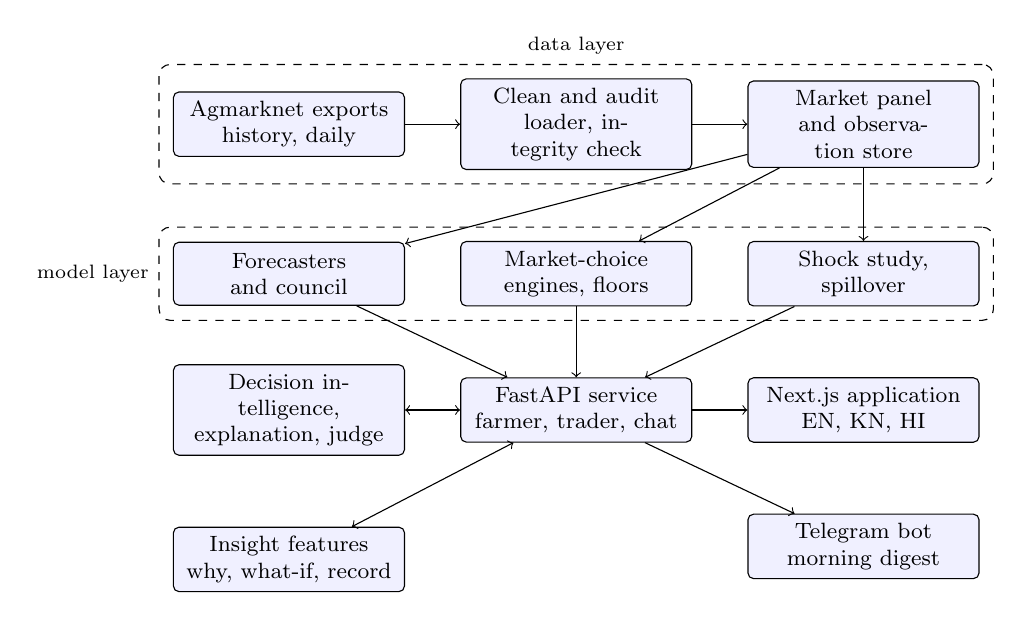
\begin{tikzpicture}[node distance=5mm and 7mm, every node/.style={font=\footnotesize}, box/.style={draw, rounded corners=2pt, align=center, minimum height=8mm, text width=2.7cm, fill=blue!6}, lay/.style={draw, dashed, rounded corners=4pt, inner sep=5pt}]
\node[box] (raw) {Agmarknet exports\\ history, daily};
\node[box, right=of raw] (clean) {Clean and audit\\ loader, integrity check};
\node[box, right=of clean] (panel) {Market panel\\ and observation store};
\node[box, below=9mm of clean] (me) {Market-choice\\ engines, floors};
\node[box, left=of me] (fc) {Forecasters\\ and council};
\node[box, right=of me] (sh) {Shock study,\\ spillover};
\node[box, below=9mm of me] (api) {FastAPI service\\ farmer, trader, chat};
\node[box, left=of api] (llm) {Decision intelligence,\\ explanation, judge};
\node[box, right=of api] (web) {Next.js application\\ EN, KN, HI};
\draw[->] (raw)--(clean); \draw[->] (clean)--(panel);
\draw[->] (panel)--(me); \draw[->] (panel)--(fc); \draw[->] (panel)--(sh);
\draw[->] (me)--(api); \draw[->] (fc)--(api); \draw[->] (sh)--(api);
\draw[<->] (llm)--(api); \draw[->] (api)--(web);
\node[box, below=9mm of llm] (ins) {Insight features\\ why, what-if, record};
\node[box, below=9mm of web] (bot) {Telegram bot\\ morning digest};
\draw[<->] (api)--(ins); \draw[->] (api)--(bot);
\begin{scope}[on background layer]
\node[lay, fit=(raw)(clean)(panel), label={[font=\scriptsize]above:data layer}] {};
\node[lay, fit=(fc)(me)(sh), label={[font=\scriptsize]left:model layer}] {};
\end{scope}
\end{tikzpicture}
\caption{Architecture of MandiSense AI: data and model layers feed a single service layer, which the language layer and the web application use.}
\label{fig:architecture}
\end{figure}

\section{Dataset Description}
\label{sec:dataset}

All results use real portal records; no synthetic data enter any result (test fixtures are arrays used only to check code). Two Agmarknet exports were used: the history export, giving an arrivals-weighted modal price and arrivals per market, crop and day from \DataFrom{} to \DataTo{} (\NhistoryRows{} rows kept after cleaning), and the daily price report from 7 November 2025, with minimum, maximum and modal price per variety. Where the two overlap on 3,307 tomato market-days they agree (Pearson $r=0.99996$, 99.97\% within 5\%). The market panel holds \NpanelRows{} mandi-days. Table~\ref{tab:dataset} gives the panel by crop. The spillover engine uses a weekly panel of five crops over 232 weeks (3 January 2021 to 1 November 2026), at one reference market per crop (Bengaluru APMC for garlic, onion and potato; Ramanagara APMC for ginger and tomato). A cell of the panel is \emph{observed} only if the market reported; nothing is imputed into the panel, and any forward-filled view carries a staleness counter.

\begin{table}[!t]
\centering
\caption{Market panel by crop. ``Eligible'' counts markets with at least 700 reported days.}
\label{tab:dataset}
\gentable{tab_dataset}
\end{table}

\section{Experimental Setup, Metrics and Baselines}
\label{sec:setup}

\noindent\textbf{Protocol.} Nested walk-forward: five outer test blocks (2024-H1 to 2026-10), each trained on earlier data only. Inside every fold, two six-month validation blocks drive hyper-parameter search with Optuna~\cite{akiba2019} (TPE; 20 trials for neural models, 25 for boosting), and a gap of $K{+}2$ days separates each training window from its validation or test block so that no four-day target overlaps. Every method receives the same budget. This follows the guidance on time-ordered evaluation~\cite{bergmeir2012,cerqueira2020}.

\noindent\textbf{Metrics.} Mean realised net revenue and regret to a hindsight oracle, with day-block bootstrap intervals~\cite{kunsch1989}; the share of the gap between the nearest-mandi rule and the oracle that a method closes; the fraction of recommendations that went to a silent market; floor violation against the nominal level; forecast skill against the no-change forecast.

\noindent\textbf{Inference.} Paired daily regret differences are tested with a moving-block bootstrap (block length 14) and Newey--West Diebold--Mariano tests~\cite{diebold1995,newey1987,harvey1997}, with Holm correction~\cite{holm1979} across all pre-specified comparisons and a model confidence set~\cite{hansen2011}.

\noindent\textbf{Baselines.} Random walk with transport costs; LightGBM~\cite{ke2017} and XGBoost~\cite{chen2016} trained on observed prices (the standard predict-then-optimise); LightGBM trained on the same realised labels (to separate better labels from a better learner); and the heuristics nearest mandi today, highest price yesterday, best seven-day mean, and farm gate.

\noindent\textbf{Language layer.} Twenty-four explanations (120 sentences) were generated, eight per language in English, Kannada and Hindi, by a writer model (gpt-oss-120b) and judged by a model of a different family (Qwen). Metrics are the share of sentences kept after the validator and judge, with 95\% intervals, and the judge's power on nine deliberately corrupted and three faithful English rewrites (reversed meaning, added claim, dropped qualifier, wrong meaning).

\noindent\textbf{Spillover.} Metrics are the number of shock episodes per source and direction, the status of each of the 40 edges, the share of variance removed with the common factor, and sign agreement between in-sample and held-out estimates.

\noindent\textbf{Insight features.} The breakdown is checked by an identity: its parts must sum to the served net revenue within Rs~1. The track record replays the back-test and must reproduce its headline numbers or it is not written. The silence tax and the crowd simulator are scenario analyses on the ingested panel and the served engine; their parameters (the silent-price fraction, the price flexibility) are stated and varied.

\noindent\textbf{Pre-specification.} The model ladder, the paired comparisons, the silence tests and the leakage protocol were fixed before tuned results were seen.

\section{Software and Hardware Requirements}
\label{sec:swhw}

\begin{table}[!t]
\centering
\caption{Software used, with versions from the locked environment}
\label{tab:software-req}
\small
\begin{tabular}{|p{3.6cm}|p{5.8cm}|p{5.0cm}|}
\hline
\textbf{Category} & \textbf{Tool / library} & \textbf{Version} \\ \hline
Language & Python & 3.12 \\ \hline
Data and statistics & NumPy, pandas, SciPy, statsmodels & 1.26.4, 2.1.4, 1.11.4, 0.14.1 \\ \hline
Learning & scikit-learn, LightGBM, XGBoost, Optuna & 1.3.2, 4.6.0, 2.0.3, as locked \\ \hline
Neural (research environment) & PyTorch, Chronos-Bolt & separate research environment \\ \hline
Backend & FastAPI, Uvicorn, Pydantic & 0.136.1, 0.46.0, 2.13.3 \\ \hline
Frontend & Next.js, React, TypeScript, Tailwind CSS & 16.2.4, 19.2.4, 5, 4 \\ \hline
Testing & pytest, vitest & 9.0.3, 3.2 \\ \hline
Language layer & Groq API: gpt-oss-120b (writer), Qwen (judge) & hosted \\ \hline
Tooling & Git, GitHub Actions, Docker, Node.js & CI workflow; Node 23 \\ \hline
Messaging & Telegram Bot API (long polling), Requests & hosted, free \\ \hline
Documents & \LaTeX{} (MiKTeX), matplotlib & 3.10.0 \\ \hline
\end{tabular}
\end{table}

\begin{table}[!t]
\centering
\caption{Hardware used for development and all experiments}
\label{tab:hardware-req}
\small
\begin{tabular}{|l|l|}
\hline
\textbf{Component} & \textbf{Specification} \\ \hline
CPU & Intel Core i9-13900HX, 24 cores / 32 threads \\ \hline
GPU & NVIDIA GeForce RTX 4060 Laptop GPU \\ \hline
RAM & 31.7 GB \\ \hline
Storage & SSD, about 180 GB free on the working drive \\ \hline
OS & Windows 11 Home \\ \hline
\end{tabular}
\end{table}

Python was chosen for its statistics and boosting ecosystem, FastAPI for typed validation and automatic API documentation, and Next.js for fast pages on weak connections (alternatives: \texttt{docs/TOOL\_CHOICES.md}).

\chapter{Project Planning and Management}
\label{ch:plan}

This chapter documents how the work was organised: the work breakdown, the dependency network and critical path, the baseline and actual schedule, who was responsible for what, the risks that were anticipated and those that occurred, and the resources used.

\noindent\textbf{How to read the figures in this chapter.} The baseline schedule was reconstructed after the fact from the Phase-1 roadmap (six phases, M1--M6) rather than recorded at the start; actual dates are taken from the repository history; hours are estimates agreed by the team, not logged time. These three facts are marked wherever they matter.

\section{Work Breakdown Structure}
\label{sec:wbs}

Figure~\ref{fig:wbs} shows the five top-level work packages and Table~\ref{tab:wbs} the leaf tasks with owners and estimated effort. Child hours sum to the parent in every row.

\begin{figure}[!b]
\centering
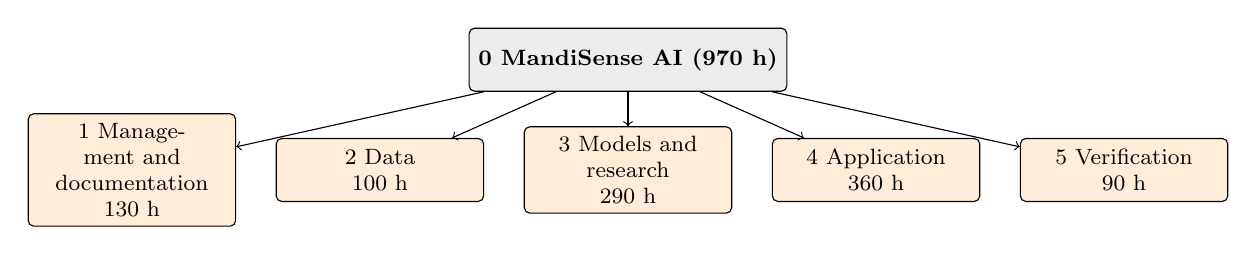
\begin{tikzpicture}[every node/.style={font=\footnotesize}, p/.style={draw, rounded corners=2pt, fill=orange!15, text width=2.4cm, align=center, minimum height=8mm}, c/.style={draw, rounded corners=2pt, fill=blue!6, text width=2.5cm, align=center, minimum height=7mm}, level distance=1.4cm, sibling distance=3.15cm, edge from parent/.style={draw, ->}]
\node[draw, fill=gray!15, rounded corners=2pt, minimum height=8mm] {\textbf{0 MandiSense AI (970 h)}}
  child {node[p] {1 Management and documentation\\130 h}}
  child {node[p] {2 Data\\100 h}}
  child {node[p] {3 Models and research\\290 h}}
  child {node[p] {4 Application\\360 h}}
  child {node[p] {5 Verification\\90 h}};
\end{tikzpicture}
\caption{Level-1 work breakdown structure with estimated hours.}
\label{fig:wbs}
\end{figure}

\begin{table}[!t]
\centering
\caption{Work breakdown with owner and estimated hours (estimates, not logged time)}
\label{tab:wbs}
\small
\begin{tabular}{|l|p{6.2cm}|l|r|}
\hline
\textbf{WBS} & \textbf{Task} & \textbf{Owner} & \textbf{Hours} \\ \hline
\textbf{1} & \textbf{Management and documentation} & & \textbf{130} \\
1.1 & Requirements and literature survey & Shreejith & 40 \\
1.2 & Planning and tracking & Shreejith & 20 \\
1.3 & Final report, appendices, similarity record & Shreejith & 70 \\ \hline
\textbf{2} & \textbf{Data} & & \textbf{100} \\
2.1 & Agmarknet acquisition & Manohara & 20 \\
2.2 & Cleaning, integrity checks, exclusions & Manohara & 40 \\
2.3 & Market panel and observation store & Manohara & 40 \\ \hline
\textbf{3} & \textbf{Models and research} & & \textbf{290} \\
3.1 & Market-choice formulation and engines, floors & Manohara & 90 \\
3.2 & Forecasters and specialist council & Manohara & 60 \\
3.3 & Experiments, statistics, leakage audit & Manohara & 100 \\
3.4 & Shock study and cross-commodity spillover & Manohara & 40 \\ \hline
\textbf{4} & \textbf{Application} & & \textbf{360} \\
4.1 & Backend API & Srijan & 90 \\
4.2 & Farmer web application & Srijan & 90 \\
4.3 & Trader web application & Srijan & 60 \\
4.4 & Decision-intelligence briefs, explanation layer, chatbot & Srijan & 60 \\ \hline
4.5 & Insight features and Telegram digest (API, pages, bot, tests) & Srijan & 60 \\ \hline
\textbf{5} & \textbf{Verification} & & \textbf{90} \\
5.1 & Test plan and validation & Shreejith & 50 \\
5.2 & Integration, pipeline, fresh-clone check & Manohara & 40 \\ \hline
\multicolumn{3}{|r|}{\textbf{Total}} & \textbf{970} \\ \hline
\end{tabular}
\end{table}

\section{Activity Network and Critical Path}
\label{sec:network}

The leaf tasks were grouped into eleven activities (Table~\ref{tab:activities}). Planned durations are in weeks; the network is in Figure~\ref{fig:network}.

\begin{table}[!t]
\centering
\caption{Activities, predecessors and planned durations}
\label{tab:activities}
\small
\begin{tabular}{|c|p{5.6cm}|c|c|c|c|c|c|}
\hline
\textbf{ID} & \textbf{Activity} & \textbf{Pred.} & \textbf{Dur.} & \textbf{ES} & \textbf{EF} & \textbf{LS} & \textbf{Slack} \\ \hline
A & Requirements and literature & --- & 2 & 0 & 2 & 0 & 0 \\ \hline
B & Data acquisition and cleaning & A & 3 & 2 & 5 & 2 & 0 \\ \hline
C & Market-choice formulation, engines & B & 4 & 5 & 9 & 5 & 0 \\ \hline
D & Backend API & A & 4 & 2 & 6 & 7 & 5 \\ \hline
E & Web application (farmer, trader) & D & 5 & 6 & 11 & 11 & 5 \\ \hline
F & Forecasters and council & C & 3 & 9 & 12 & 9 & 0 \\ \hline
G & Experiments, statistics, leakage & C, F & 4 & 12 & 16 & 12 & 0 \\ \hline
H & Decision intelligence, explanation layer, chatbot & D & 3 & 6 & 9 & 13 & 7 \\ \hline
I & Testing and validation & E, G, H & 3 & 16 & 19 & 16 & 0 \\ \hline
J & Integration and reproducibility & I & 2 & 19 & 21 & 19 & 0 \\ \hline
K & Report and documentation & J & 3 & 21 & 24 & 21 & 0 \\ \hline
\end{tabular}
\end{table}

\begin{figure}[!t]
\centering
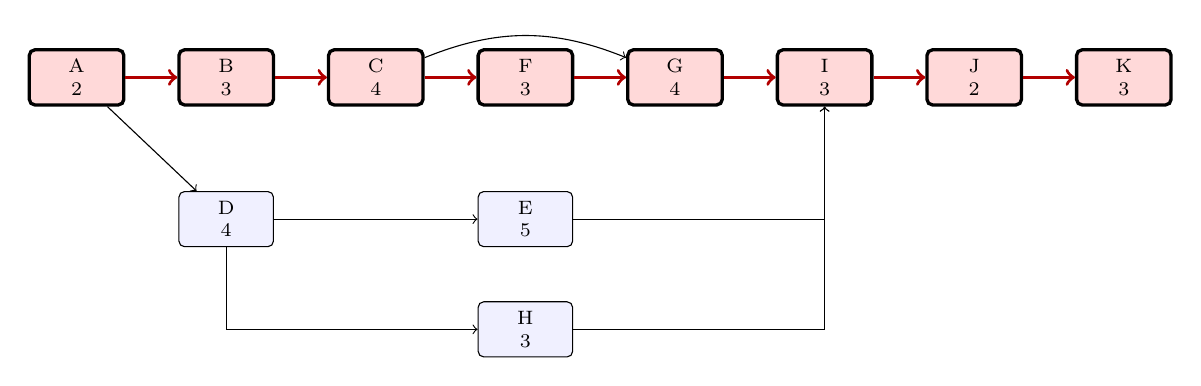
\begin{tikzpicture}[every node/.style={font=\scriptsize}, n/.style={draw, rounded corners=2pt, minimum width=1.2cm, minimum height=7mm, align=center}, cr/.style={n, fill=red!15, very thick}, nc/.style={n, fill=blue!6}]
\node[cr] (A) at (0,0) {A\\2};
\node[cr] (B) at (1.9,0) {B\\3};
\node[cr] (C) at (3.8,0) {C\\4};
\node[cr] (F) at (5.7,0) {F\\3};
\node[cr] (G) at (7.6,0) {G\\4};
\node[cr] (I) at (9.5,0) {I\\3};
\node[cr] (J) at (11.4,0) {J\\2};
\node[cr] (K) at (13.3,0) {K\\3};
\node[nc] (D) at (1.9,-1.8) {D\\4};
\node[nc] (E) at (5.7,-1.8) {E\\5};
\node[nc] (H) at (5.7,-3.2) {H\\3};
\draw[->, very thick, red!70!black] (A)--(B); \draw[->, very thick, red!70!black] (B)--(C); \draw[->, very thick, red!70!black] (C)--(F);
\draw[->, very thick, red!70!black] (F)--(G); \draw[->, very thick, red!70!black] (G)--(I); \draw[->, very thick, red!70!black] (I)--(J); \draw[->, very thick, red!70!black] (J)--(K);
\draw[->] (A)--(D); \draw[->] (D)--(E); \draw[->] (D)|-(H);
\draw[->] (C) to[bend left=22] (G);
\draw[->] (E)-|(I); \draw[->] (H)-|(I);
\end{tikzpicture}
\caption{Activity-on-node network. The critical path A--B--C--F--G--I--J--K is shown in red; durations are in weeks.}
\label{fig:network}
\end{figure}

\noindent\textbf{Worked calculation.} The forward pass gives $EF_K=24$ weeks, which is the planned duration. For the backward pass, $LF_K=24$ and $LS_K=24-3=21$; $LS_J=21-2=19$; $LS_I=19-3=16$; $LS_G=16-4=12$; $LS_F=12-3=9$; $LS_C=\min(LS_F,LS_G)-4=9-4=5$; $LS_B=2$; $LS_A=0$. The path with zero slack is therefore A--B--C--F--G--I--J--K, of length $2+3+4+3+4+3+2+3=24$ weeks. For activity E, $LF_E=LS_I=16$, so $LS_E=16-5=11$ and slack $=LS_E-ES_E=11-6=5$ weeks. For H, $LS_H=16-3=13$ and slack $=13-6=7$. For D, $LF_D=\min(LS_E,LS_H)=\min(11,13)=11$, so $LS_D=7$ and slack $=7-2=5$.

\noindent\textbf{Consequence.} The application work (D, E, H) had slack and the research chain did not. In practice the research chain was reopened late (Section~\ref{sec:risks}), which is why the project overran.

\section{Schedule: Baseline against Actual}
\label{sec:gantt}

The baseline runs 24 weeks from 27 April 2026 (week 0) and was reconstructed from the Phase-1 roadmap. Actual spans come from commit dates (first commit 28 April 2026, last 29 October 2026); the repository shows no activity between 10 June and 28 September, so the bars for E and D show continuous spans that include that gap. Total slip is about 3.3 weeks (14\% over the 24-week baseline). The insight features and the Telegram digest were added after the research results were complete; they are outside the 24-week baseline and add an estimated 60 hours (Table~\ref{tab:wbs}).

\begin{figure}[!t]
\centering
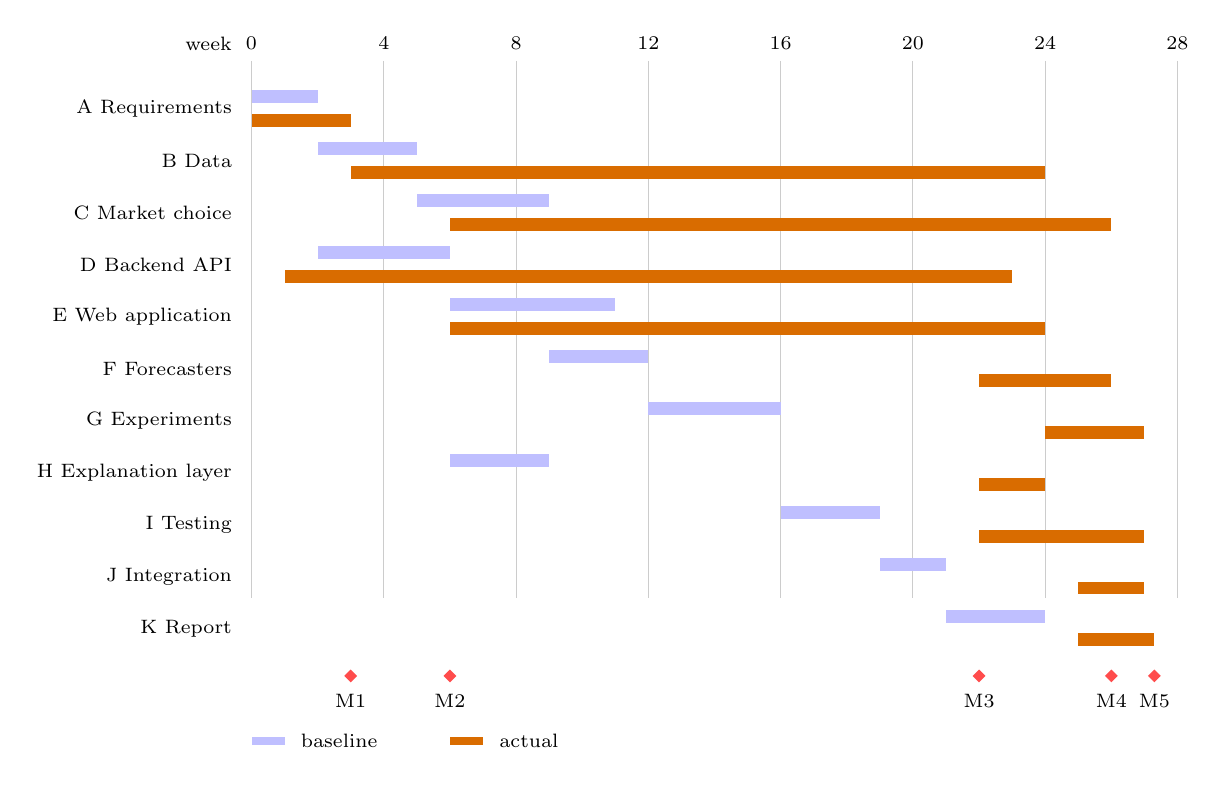
\begin{tikzpicture}[x=0.42cm, y=0.55cm, font=\scriptsize]
\foreach \w in {0,4,...,28} {\draw[gray!40] (\w,0.6) -- (\w,-11.8); \node at (\w,1) {\w};}
\node[anchor=east] at (-0.3,1) {week};
\def\row#1#2#3#4#5#6{\node[anchor=east] at (-0.3,-#1) {#2}; \fill[blue!25] (#3,-#1+0.12) rectangle (#4,-#1+0.42); \fill[orange!85!black] (#5,-#1-0.42) rectangle (#6,-#1-0.12);}
\row{0.5}{A Requirements}{0}{2}{0}{3}
\row{1.7}{B Data}{2}{5}{3}{24}
\row{2.9}{C Market choice}{5}{9}{6}{26}
\row{4.1}{D Backend API}{2}{6}{1}{23}
\row{5.3}{E Web application}{6}{11}{6}{24}
\row{6.5}{F Forecasters}{9}{12}{22}{26}
\row{7.7}{G Experiments}{12}{16}{24}{27}
\row{8.9}{H Explanation layer}{6}{9}{22}{24}
\row{10.1}{I Testing}{16}{19}{22}{27}
\row{11.3}{J Integration}{19}{21}{25}{27}
\row{12.5}{K Report}{21}{24}{25}{27.3}
\foreach \m/\l in {3/M1,6/M2,22/M3,26/M4,27.3/M5} {\node[diamond, fill=red!70, inner sep=1.2pt] at (\m,-13.6) {}; \node[below] at (\m,-13.8) {\l};}
\fill[blue!25] (0,-15.2) rectangle (1,-15); \node[anchor=west] at (1.2,-15.1) {baseline};
\fill[orange!85!black] (6,-15.2) rectangle (7,-15); \node[anchor=west] at (7.2,-15.1) {actual};
\end{tikzpicture}
\caption{Baseline (blue) against actual (orange) schedule. Milestones: M1 requirements and literature complete (week 3); M2 first deployed prototype, 9 June (week 6); M3 farmer feature suite, 30 September (week 22); M4 research results and release, 29 October (week 26); M5 final report (week 27).}
\label{fig:gantt}
\end{figure}

\begin{table}[!t]
\centering
\caption{Schedule variance by activity (weeks from 27 April 2026; actual spans from commits)}
\label{tab:variance}
\small
\begin{tabular}{|c|c|c|c|c|p{4.6cm}|}
\hline
\textbf{ID} & \textbf{Baseline} & \textbf{Actual} & \textbf{Finish slip} & \textbf{On critical path} & \textbf{Reason} \\ \hline
A & 0--2 & 0--3 & +1 & yes & Scope clarified after first review \\ \hline
B & 2--5 & 3--24 & +19 & yes & Data reopened (Sec.~\ref{sec:risks}, R1) \\ \hline
C & 5--9 & 6--26 & +17 & yes & Re-specified on real labels \\ \hline
D & 2--6 & 1--23 & +17 & no & Slack absorbed it \\ \hline
E & 6--11 & 6--24 & +13 & no & Farmer suite added in September \\ \hline
G & 12--16 & 24--27 & +11 & yes & Waited for rebuilt panel \\ \hline
K & 21--24 & 25--27.3 & +3.3 & yes & Project finish \\ \hline
\end{tabular}
\end{table}

\section{Responsibility Assignment Matrix}
\label{sec:ram}

Table~\ref{tab:ram} assigns each work package using R (responsible), A (accountable), C (consulted), I (informed). The guide is accountable for approval of each package. The split matches the owners in Table~\ref{tab:wbs}.

\begin{table}[!t]
\centering
\caption{RACI matrix by work package}
\label{tab:ram}
\small
\begin{tabular}{|l|c|c|c|c|}
\hline
\textbf{Package} & \textbf{Manohara} & \textbf{Srijan} & \textbf{Shreejith} & \textbf{Guide} \\ \hline
1 Management and documentation & C & C & R & A \\ \hline
2 Data & R & I & C & A \\ \hline
3 Models and research & R & C & C & A \\ \hline
4 Application & C & R & I & A \\ \hline
5 Verification & R (5.2) & C & R (5.1) & A \\ \hline
\end{tabular}
\end{table}

Hours by owner follow from Table~\ref{tab:wbs}: Manohara 430, Srijan 360, Shreejith 180, a total of 970.

\noindent\textbf{Contribution record.} The repository's commit history (\texttt{docs/CONTRIBUTIONS.md}) shows 64 commits by Manohara, 1 by Srijan and none by Shreejith. The owners above are the team's agreed split; the history does not corroborate the work of the second and third members, and work done on other machines would not appear in it.

\section{Risk Register}
\label{sec:risks}

\begin{table}[!t]
\centering
\caption{Risk register. Probability (P) and impact (I) on a 1--5 scale; exposure E $=$ P$\times$I. Status shows whether the risk occurred.}
\label{tab:risks}
\small
\begin{tabular}{|c|p{4.1cm}|c|c|c|p{4.0cm}|p{2.7cm}|}
\hline
\textbf{ID} & \textbf{Risk} & \textbf{P} & \textbf{I} & \textbf{E} & \textbf{Mitigation / response} & \textbf{Status} \\ \hline
R1 & Source data not real: the first dataset in the repository was synthetic & 3 & 5 & 15 & Re-acquired Agmarknet exports; integrity check between exports; synthetic removed & \textbf{Occurred} \\ \hline
R2 & Look-ahead leakage in features or evaluation & 4 & 5 & 20 & Leakage unit tests; causal protocol & \textbf{Occurred}; two whole-series-centred features, caught by test \\ \hline
R3 & Hard deletion of records breaks trader pages & 3 & 3 & 9 & Soft delete and re-seeding & \textbf{Occurred} \\ \hline
R4 & Dependency break (NumPy upgrade) & 3 & 3 & 9 & Pinned NumPy 1.26.4, regenerated lock file & \textbf{Occurred} \\ \hline
R5 & LLM API rate limit (8,000 tokens per minute) & 4 & 2 & 8 & Throttling; small evaluation set & \textbf{Occurred} \\ \hline
R6 & Uneven contribution within the team & 3 & 4 & 12 & Contribution record; owner split; guide review & Open \\ \hline
R7 & Public deployment not verified end to end & 3 & 3 & 9 & Docker and Render files provided; not tested live & Open \\ \hline
R8 & No field trial with farmers & 4 & 3 & 12 & Stated as limitation; survey instrument ready & Open \\ \hline
R9 & Agmarknet changes export format & 2 & 4 & 8 & Loader rejects unexpected units and keys & Not occurred \\ \hline
R10 & Stale development servers answered with old code while new features were tested & 3 & 2 & 6 & Restart after every change; smoke test lists every new endpoint and page & \textbf{Occurred} \\ \hline
\end{tabular}
\end{table}

\noindent\textbf{Risk R1 in detail.} The most costly event was the discovery that the first dataset in the repository was synthetic and that results derived from it had no meaning. It was found late in the project. The response was to discard it, rebuild the panel from the portal exports, and re-run every experiment. This is the main cause of the slip in B, C and G (Table~\ref{tab:variance}), and it is why critical-path activities, not slack activities, absorbed the delay.

\section{Resources and Cost}
\label{sec:cost}

\begin{table}[!t]
\centering
\caption{Resource and cost summary. Labour is notional at Rs 200 per hour; no cash was paid for it.}
\label{tab:cost}
\small
\begin{tabular}{|l|p{6.2cm}|r|r|}
\hline
\textbf{Resource} & \textbf{Basis} & \textbf{Units} & \textbf{Cost (Rs)} \\ \hline
Labour -- Manohara & 430 h at Rs 200 & 430 & 86,000 \\ \hline
Labour -- Srijan & 360 h at Rs 200 & 360 & 72,000 \\ \hline
Labour -- Shreejith & 180 h at Rs 200 & 180 & 36,000 \\ \hline
Compute & Team laptop (Table~\ref{tab:hardware-req}), already owned & --- & 0 \\ \hline
Data & Agmarknet public portal & --- & 0 \\ \hline
Language model API & Free tier of the provider & --- & 0 \\ \hline
Hosting & Free tiers (deployment not verified) & --- & 0 \\ \hline
\textbf{Total notional} & & 970 & \textbf{1,94,000} \\ \hline
\textbf{Cash spent} & & & \textbf{0} \\ \hline
\end{tabular}
\end{table}

Labour totals match the hours in Table~\ref{tab:wbs}. No tool or service with a licence fee was used.

\chapter{Implementation}
\label{ch:impl}

This chapter describes how the method of Chapter~\ref{ch:method} was realised in code, how the parts were joined into one system, and how the system was tested. Source code excerpts are in Appendix~\ref{appendix:code}.

\section{Algorithm Implementation}
\label{sec:algorithm-implementation}

\subsection{Panel construction and leakage control}

The loader (\texttt{research/gfmc/data/loader.py}) parses the portal exports, drops the footer rows, rejects unexpected units, checks key uniqueness and records a load report of rows read, dropped and kept. The panel builder then forms one row per market and day with the arrivals-weighted modal price, a reported flag, and a staleness counter. Features at index $s$ use only data up to $s-1$: lags and spreads of the price, cross-market spreads, arrivals, own staleness and report rate, and calendar terms. Targets are strictly future prices. A unit test (Section~\ref{sec:testing-validation}) perturbs the future and checks that features do not move; it caught a defect during development, in which two features were centred on a whole-series mean.

\subsection{Market-choice models}

Revenue labels follow Equation~\ref{eq:revenue} for the 49 actions (12 markets $\times$ 4 holds, plus the farm gate), for five farmer origins. Gradient-boosted models are trained per action on the labels; the neural model is the DeepSets network of Section~\ref{sec:proposed} trained with Equation~\ref{eq:spo}. The served engines, one per crop, are the boosted models on realised-revenue labels, because they were statistically indistinguishable from the neural variant (Section~\ref{sec:effects}) and cheaper to run and explain.

\subsection{Floors with delayed feedback}

The floor procedure (\texttt{mandisense\_ai/market\_choice/conformal.py}) is an online loop over decision days. An outcome from a $k$-day hold is added to the score pool only when its sale date is strictly in the past; the conformal quantile of the pool sets $q$, and $\alpha_t$ is updated by Equation~\ref{eq:aci}. Below the minimum of 30 resolved scores a default multiplier is used and the floor is flagged as uncalibrated.

\subsection{Forecasters and the specialist council}

District price forecasters at 3, 5 and 7 days are served only when a horizon beats the no-change forecast on held-out folds; horizons that do not are marked not served. The council splits the feature set into four families, trains one agent per family, and combines their forecasts with non-negative weights constrained to sum to at most one, fitted fold by fold. The first version, without the constraint, produced weights summing to \CouncilUnconstrainedSum{} and was significantly worse than a single model; the constrained version is the one reported.

\subsection{Decision-intelligence service}

The service (\texttt{mandisense\_ai/intelligence/}) has four steps, each in its own module. \emph{Evidence} (\texttt{evidence.py}) gathers the facts for one crop and market into a flat map keyed by dotted paths, such as \texttt{forecast.h5.point}, \texttt{forecast.h5.net\_change\_after\_spoilage\_pct}, and the market-choice and spillover entries, and records what was unavailable and why. \emph{Providers} (\texttt{providers.py}) fill the brief schema of \texttt{schema.py}: a hosted language model through a tool definition (Claude or the Groq-hosted gpt-oss model, selected by configuration) or a deterministic provider that writes the same brief from rules. The schema is the contract: an action from \{BUY, SELL, HOLD, WAIT\}, a confidence level that may be INSUFFICIENT\_EVIDENCE, and factors that each cite an evidence key. \emph{Grounding} (\texttt{grounding.py}) parses every number in the brief and checks it against the evidence (Algorithm~\ref{alg:grounding}); ordinary small integers are ignored, and a brief may name only the markets that appear in its own evidence, which stops a model from quietly recommending a market the engine did not. \emph{Service} (\texttt{service.py}) ties these together and never raises into a request: a failing provider falls back to the deterministic one, and an ungrounded brief is still returned, marked \texttt{grounded: false} with its issues listed, because a visible failure is more useful to the operator than a silent one.

\begin{algorithm}[!t]
\caption{Grounding verification of a decision brief}
\label{alg:grounding}
\begin{algorithmic}[1]
\Require Brief $B$, evidence bundle $E$ (key $\rightarrow$ value)
\Ensure List of issues (empty if grounded)
\State $\mathcal{I}\gets\emptyset$
\For{each factor $f$ in $B$}
    \If{$f.\text{evidence\_ref}\notin E$} \State add ``unknown evidence key'' to $\mathcal{I}$ \EndIf
\EndFor
\For{each number $x$ in the prose of $B$ (headline, rationale, factor details, risks, watch-next)}
    \If{$|x|<32$ \textbf{or} $x$ is part of a market name} \State \textbf{continue} \EndIf
    \If{no value $v\in E$ has $|x-v|\le 0.01\,|v|$} \State add ``figure not in evidence: $x$'' to $\mathcal{I}$ \EndIf
\EndFor
\For{each known mandi name $n$ that appears in the prose}
    \If{$n$ does not appear in the evidence} \State add ``names $n$, which is not in the evidence'' to $\mathcal{I}$ \EndIf
\EndFor
\State \Return $\mathcal{I}$
\end{algorithmic}
\end{algorithm}

\subsection{Explanation writer and judge}

Separately from the brief, explanation sentences written by code (the best market, the floor, the reasons) may be rephrased in the farmer's language. The writer model (gpt-oss-120b) receives the sentence and the numbers it contains; a validator rejects any output whose numbers differ, that adds a digit, uses an overclaim word, is too long or is in the wrong script; an independent judge model (Qwen) then checks faithfulness. A rejected sentence falls back to the original text, so this layer cannot change a number.

\subsection{Cross-commodity spillover engine}

The engine (\texttt{mandisense\_ai/spillover/}) is a pure offline build whose output is a versioned artefact, \texttt{spillover\_matrix.json}, that records the data hash, the configuration and diagnostics with the edges. \texttt{panel.py} resamples the five crops to weekly series at their reference markets; \texttt{common\_factor.py} removes the first principal component (leave-one-out) and calendar-month means; \texttt{events.py} detects shock episodes from the supply-regime labels (squeeze or glut) and merges onsets less than four weeks apart; \texttt{estimator.py} computes Equation~\ref{eq:spill} at horizons of one to four weeks with an episode bootstrap of 2,000 draws; \texttt{matrix.py} applies the Benjamini--Hochberg correction across all edges and the publication gates; and \texttt{validate.py} performs the holdout sign-agreement check. The random seed and every threshold live in one configuration object that is stored in the artefact, so a rebuild on unchanged data reproduces the file exactly. At run time \texttt{SpilloverService} reads the artefact and fails safe: if it is missing or stale, the brief states that spillover evidence is unavailable.

\subsection{Insight features}

All five features live in one module (\texttt{mandisense\_ai/market\_choice/insights.py}) that reads the served engine and the ingested panel and fits nothing at request time. The breakdown re-expresses the served net revenue as its parts (Equation~\ref{eq:breakdown}) and \emph{asserts} that they add up within Rs~1, so it cannot drift from the advice it explains. The what-if function re-prices every action under new costs from the model's own predicted prices and sweeps transport and spoilage over a grid to find where the best action changes. The crowd function scales a yard's price with the quantity it receives (Equation~\ref{eq:crowd}) and splits the quantity greedily on marginal revenue. The silence tax is computed from the last year of the panel (Equation~\ref{eq:silence}). The track record is built offline by \texttt{scripts/build\_track\_record.py}, which replays the back-test with daily output and \emph{refuses to write} if its headline numbers disagree with the engine's own; it is a stage of the pipeline.

On the farmer side the first three appear as collapsible panels inside the Best Place and Day to Sell tool, fetched only when opened, so the advice itself is never delayed (Figure~\ref{fig:ui-insight}); their words exist in English, Kannada and Hindi and are tested for completeness. On the trader side the silence tax and the crowd simulator are two tools of the desk. Code excerpts are in Appendix~\ref{appendix:code}.

\begin{figure}[!t]
\centering
\begin{minipage}[t]{0.485\textwidth}\centering\fbox{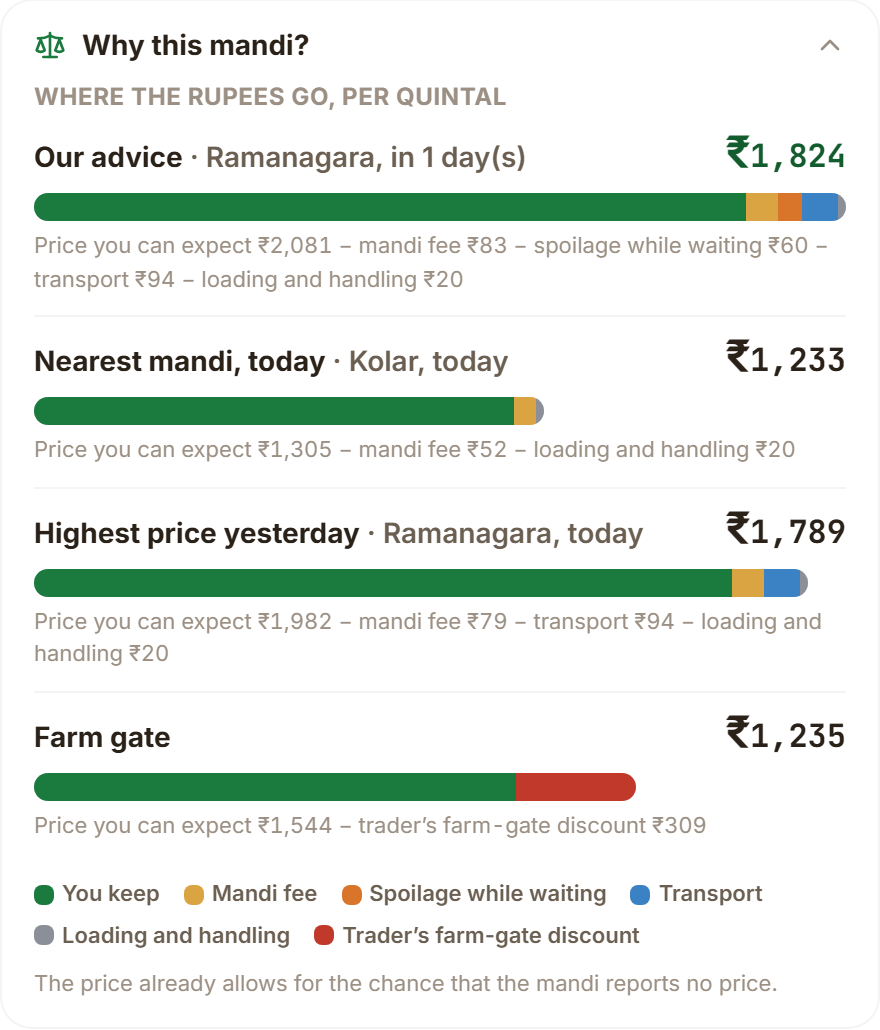
\includegraphics[width=0.94\linewidth]{figures/ins_farmer_why.png}}\\[1mm]{\small (a) Why this mandi?}\end{minipage}\hfill
\begin{minipage}[t]{0.485\textwidth}\centering\fbox{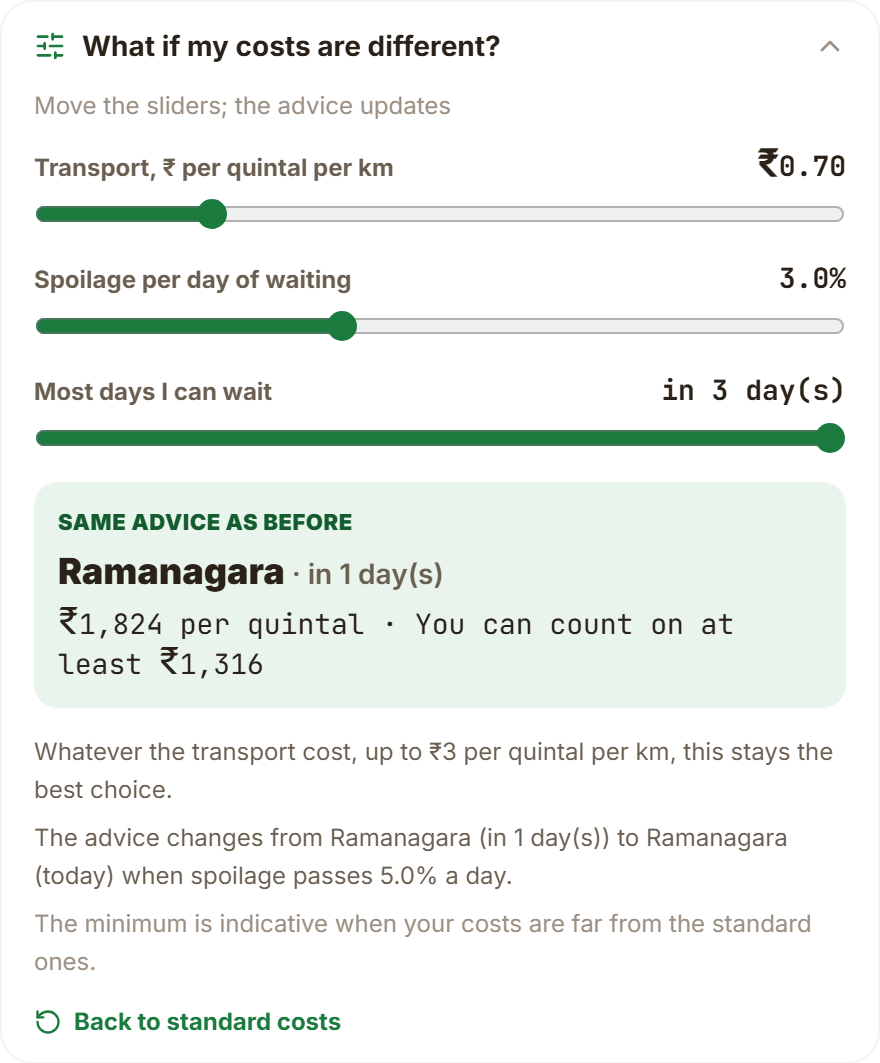
\includegraphics[width=0.94\linewidth]{figures/ins_farmer_whatif.png}}\\[1mm]{\small (b) What if my costs differ?}\end{minipage}
\medskip
\begin{minipage}[t]{0.485\textwidth}\centering\fbox{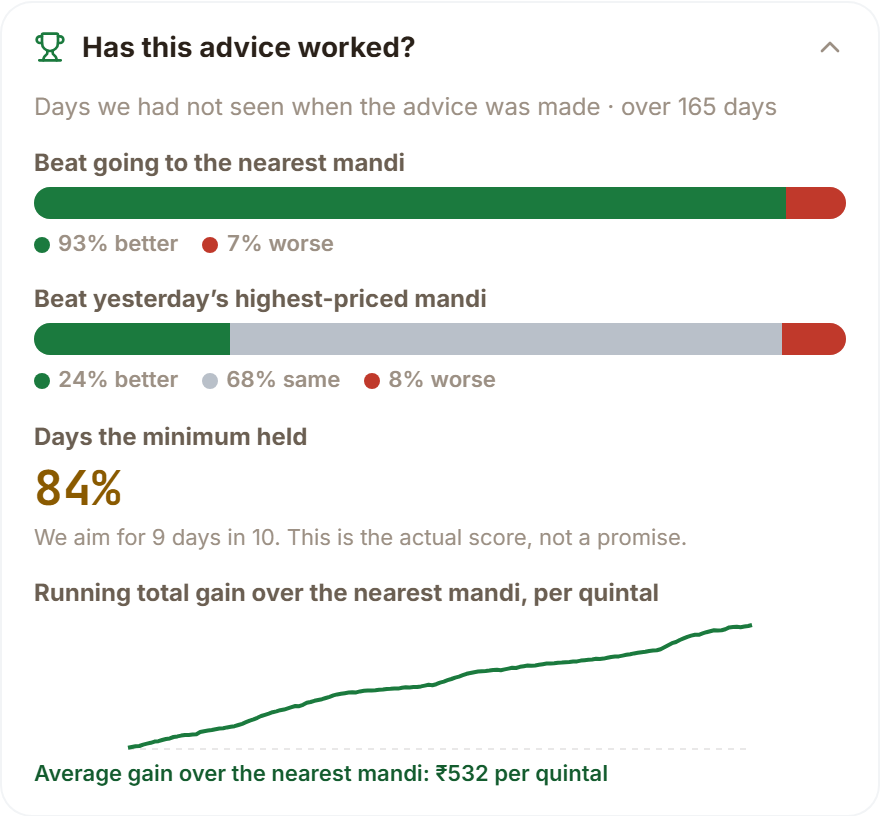
\includegraphics[width=0.94\linewidth]{figures/ins_farmer_score.png}}\\[1mm]{\small (c) Has this advice worked?}\end{minipage}
\caption{The three farmer panels inside the Best Place and Day to Sell tool, for tomato in Kolar, with real data. In (b) the advice changes when spoilage passes 5\% a day.}
\label{fig:ui-insight}
\end{figure}

\subsection{Daily digest and Telegram bot}

The digest builder (\texttt{mandisense\_ai/notify/digest.py}) turns the panel and the engines into one message (Section~\ref{sec:digest-method}). The bot (\texttt{mandisense\_ai/notify/telegram.py}) uses the Telegram Bot API over HTTPS with long polling, so it runs on a laptop with no public address. A farmer presses Start, chooses a language, a district and crops with buttons and receives the first digest at once; \texttt{/today} repeats it, \texttt{/stop} unsubscribes, and typing a crop and a place (``tomato kolar'', or the same in Kannada or Hindi) returns the digest for them. Subscribers and an append-only log of every attempt (sent, failed, with message identifiers) are kept in two files beside the other farmer stores, and a blocked bot marks the subscriber inactive. A script (\texttt{scripts/send\_daily\_digest.py}) sends the morning digest to every active subscriber and has a dry-run mode; scheduled for 07:00 it is the daily message. The bot's token is read from the environment, never logged or committed.

\subsection{Use of AI assistance}
\label{sec:ai-disclosure}
The authors used Anthropic's Claude~\cite{claude3} through the Claude Code command-line assistant as a development and writing aid: for drafting and refactoring code, writing tests, generating the figures and tables from stored experiment results, searching and checking bibliographic records against public indices, and drafting and copy-editing text. The design decisions, experiments, numbers and conclusions are the authors' own; every number in the thesis is produced by scripts from stored artefacts, and every reference was checked against Crossref or arXiv before it was listed. The product itself does not call Claude: its explanation writer and judge are the open-weight models named in Section~\ref{sec:llm}.

\section{System Integration}
\label{sec:system-integration}

\subsection{Pipeline}

One script (\texttt{scripts/pipeline.py}) runs the stages in dependency order: building the farmer world, seeding and running forecasts, building the market-choice engines, the day-by-day track record of the advice, transmission, shock study, spillover, council evaluation, research evidence export, results document, and (optionally) the full research experiments and LLM evaluation, ending with the tests. Each stage is a command with declared outputs, so a stage can be run alone, skipped, or dry-run. Figure~\ref{fig:integration-flow} shows the flow.

\begin{figure}[!t]
\centering
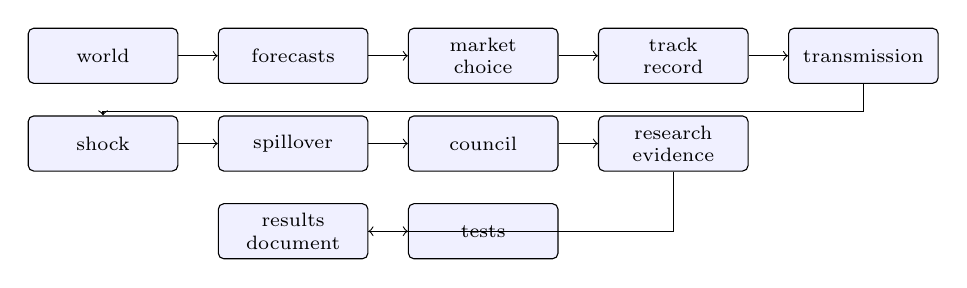
\begin{tikzpicture}[node distance=4mm and 5mm, every node/.style={font=\scriptsize}, s/.style={draw, rounded corners=2pt, fill=blue!6, minimum width=1.9cm, minimum height=7mm, align=center}]
\node[s] (w) {world};
\node[s, right=of w] (f) {forecasts};
\node[s, right=of f] (m) {market\\choice};
\node[s, right=of m] (tr) {track\\record};
\node[s, right=of tr] (t) {transmission};
\node[s, below=of w] (sh) {shock};
\node[s, right=of sh] (sp) {spillover};
\node[s, right=of sp] (c) {council};
\node[s, right=of c] (r) {research\\evidence};
\node[s, below=of sp] (res) {results\\document};
\node[s, right=of res] (te) {tests};
\draw[->] (w)--(f); \draw[->] (f)--(m); \draw[->] (m)--(tr); \draw[->] (tr)--(t);
\draw[->] (t.south) -- ++(0,-0.35) -| (sh.north);
\draw[->] (sh)--(sp); \draw[->] (sp)--(c); \draw[->] (c)--(r);
\draw[->] (r.south) |- (res.east); \draw[->] (res)--(te);
\end{tikzpicture}
\caption{Stages of the reproducible pipeline, in the order they run.}
\label{fig:integration-flow}
\end{figure}

\subsection{Service and application}
\label{sec:service-app}

The FastAPI application mounts routers for market choice (\texttt{/v1/market-choice}), farmer tools (\texttt{/v1/farmer}), trader tools (\texttt{/v1/trader}), supply shocks (\texttt{/v1/shock}), the council (\texttt{/v1/council}), cross-commodity spillover (\texttt{/v1/spillover}), forecasts, chat, decision intelligence (\texttt{/v1/intelligence}), the five insight endpoints under \texttt{/v1/market-choice}, and the notification routes (\texttt{/v1/notify}). Request and response models are typed with Pydantic, so a malformed request is rejected before it reaches a model. The Next.js application calls these endpoints; Figure~\ref{fig:ui-farmer} shows the farmer home in Kannada and the market-choice desk for traders.

\begin{figure}[!t]
\centering
\begin{minipage}[c]{0.27\textwidth}\centering
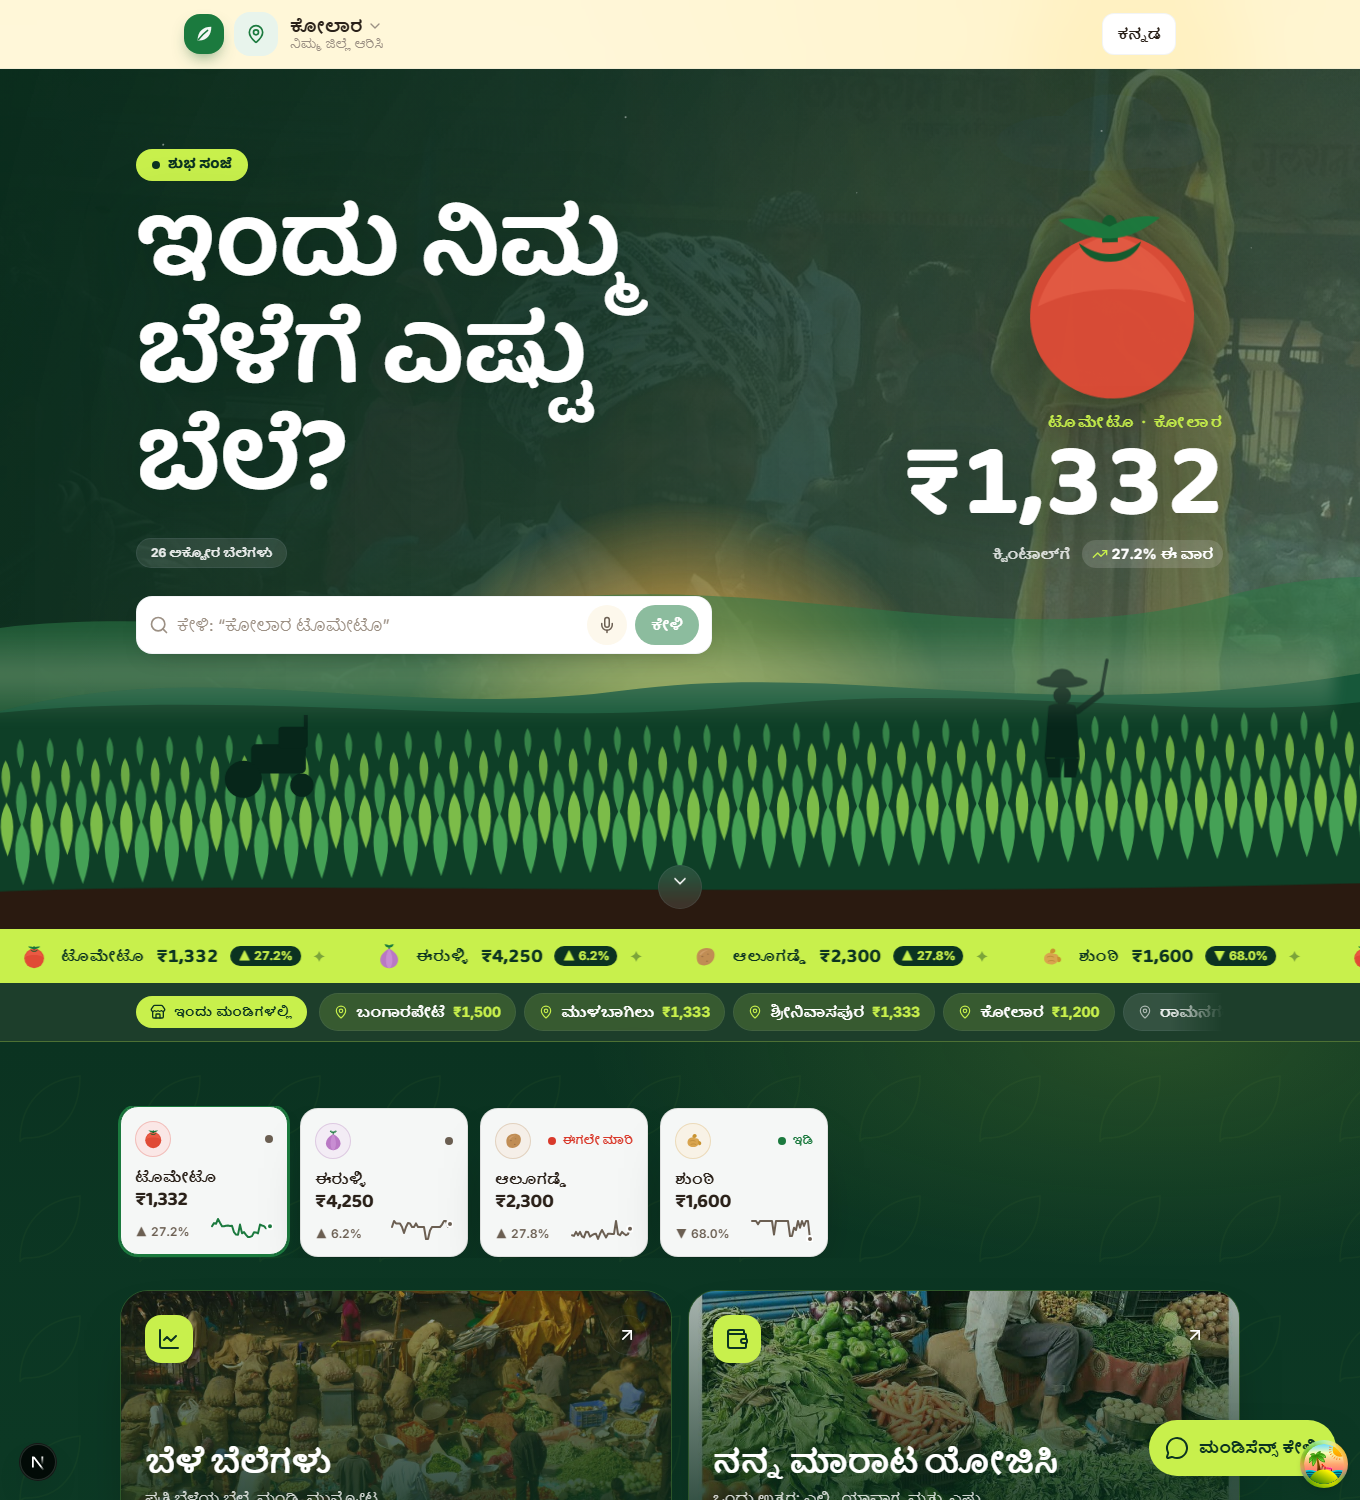
\includegraphics[height=10.4cm]{figures/ui_farmer_home.png}\\[1mm]{\small (a) Farmer home, Kannada}
\end{minipage}\hfill
\begin{minipage}[c]{0.70\textwidth}\centering
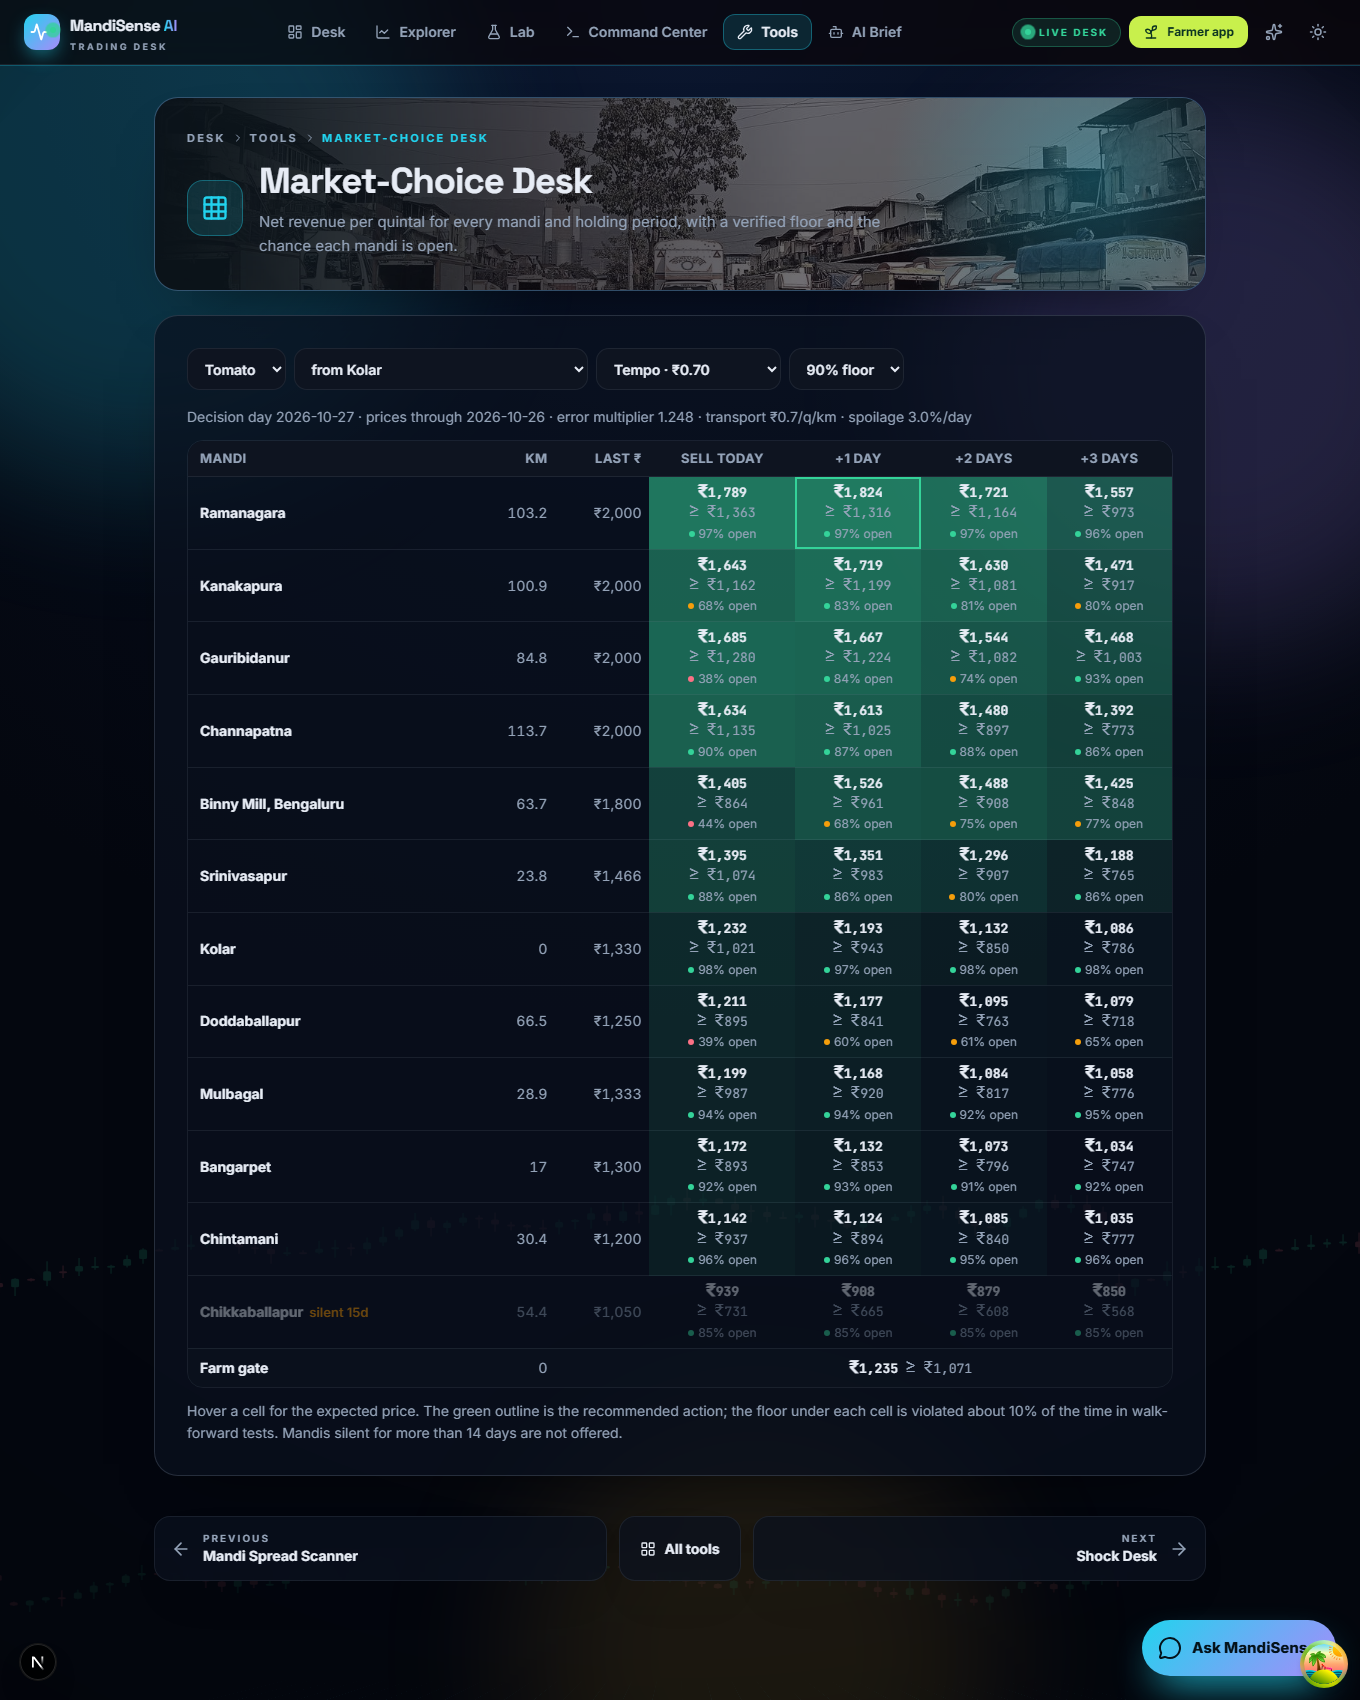
\includegraphics[width=\textwidth]{figures/ui_market_choice.png}\\[1mm]{\small (b) Market-choice desk}
\end{minipage}
\caption{(a) The farmer home screen in Kannada, showing today's best place to sell and the reasons for it. (b) The market-choice desk for traders: recommended market and holding period, the verified floor and the evidence level for the crop. Both are rendered from real data.}
\label{fig:ui-farmer}
\end{figure}

\subsection{Challenges and solutions}
Table~\ref{tab:challenges} lists the integration problems met while joining the parts and how each was resolved.

\begin{table}[H]
\centering
\caption{Integration problems met and how they were resolved}
\label{tab:challenges}
\small
\begin{tabular}{|p{4.6cm}|p{5.2cm}|p{4.6cm}|}
\hline
\textbf{Problem} & \textbf{Cause} & \textbf{Resolution} \\ \hline
Pandas failed to import after installing a plotting library & The installer upgraded NumPy to 2.5, incompatible with pandas 2.1.4 & Pinned NumPy 1.26.4; regenerated the lock file; dependency check clean \\ \hline
Ginger experiment found no rows & Export names the crop ``Ginger(Green)'' & Added a source-name alias in the configuration \\ \hline
Fresh clone failed three tests and skipped four & The observation store was untracked & Tracked the store; pipeline seeds history; tests guarded \\ \hline
Trader pages empty after a data refresh & Hard deletion of records broke references & Re-seeding and id aliasing \\ \hline
Council weights summed to more than 1 & Unconstrained non-negative least squares & Constrained sum to at most one; unconstrained kept as a reported column \\ \hline
Language-layer calls throttled & Provider limit of 8,000 tokens per minute & Request throttling; small evaluation set \\ \hline
Silence tax read as zero for a cheap, unreliable mandi & Its usual price is below the fallback price, so silence costs no money on price & Added a surprise-silence column and a note that zero is not reliability \\ \hline
New endpoints answered ``not found'' in testing & A server started before the change was still running old code & Restarted it; the smoke test lists every new endpoint and page \\ \hline
\end{tabular}
\end{table}

\section{System Walkthrough with Screenshots}
\label{sec:screens}

This section shows the running system. Every figure is a screenshot of the web application served from the stored data of the final system (market prices up to 26 October 2026), captured by a script (\texttt{report/capture\_system.py}) driving a headless browser, so the figures can be regenerated and are not edited. The farmer interface is shown at phone width because that is how most farmers will use it; the trader desk is shown at desktop width. Prices are in rupees per quintal unless stated, and every price on screen carries the date it was reported.

\subsection{Farmer interface}
The farmer interface is built around a single question, ``what is my crop worth today, and where should I sell it?''. It has a language switch (English, Kannada, Hindi), a district selector and a bottom navigation bar with Home, Prices and Tools.


\begin{figure}[!t]
\centering
\begin{minipage}[t]{0.485\textwidth}\centering\fbox{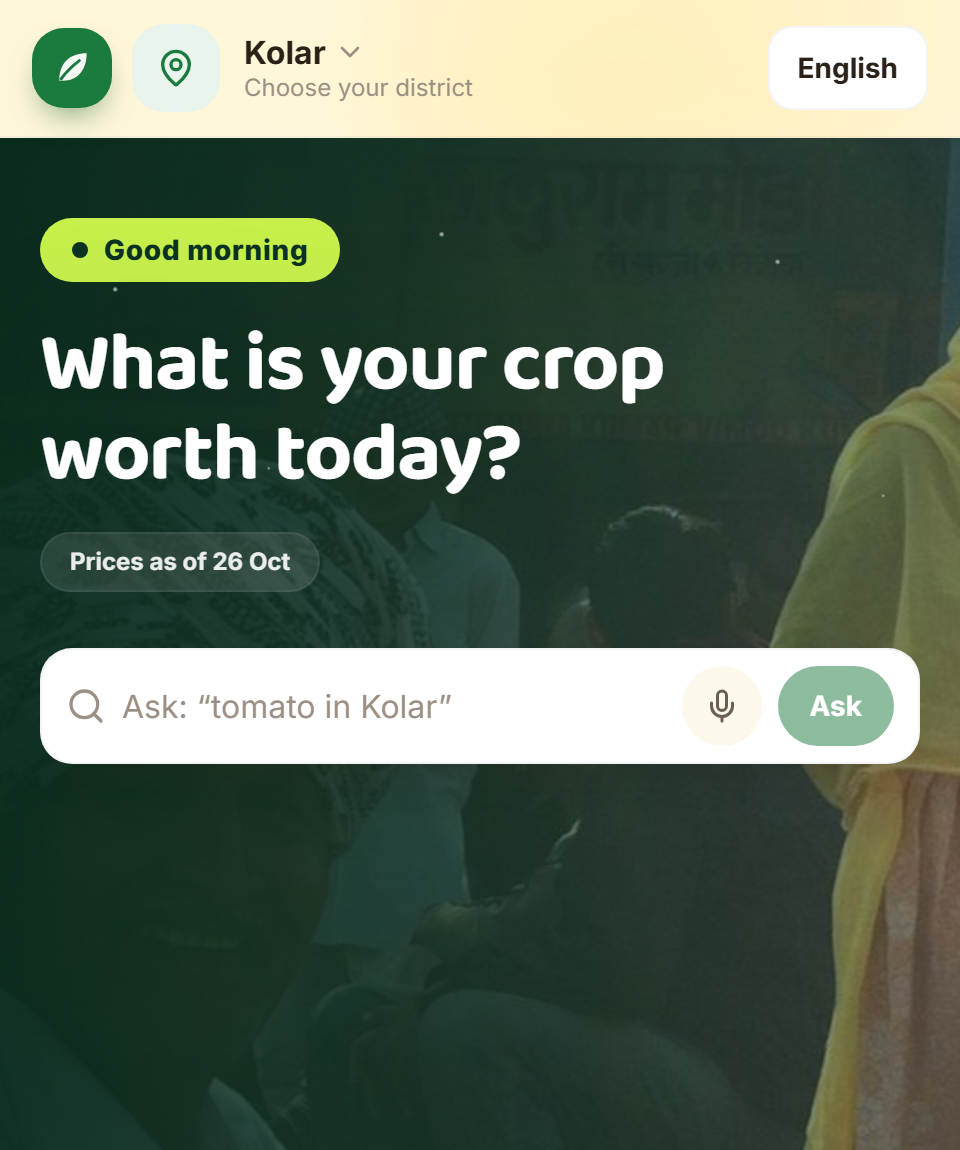
\includegraphics[width=0.94\linewidth,height=9.0cm,keepaspectratio]{figures/shot_f_home.png}}\\[1mm]{\footnotesize (a) Home}\end{minipage}\hfill
\begin{minipage}[t]{0.485\textwidth}\centering\fbox{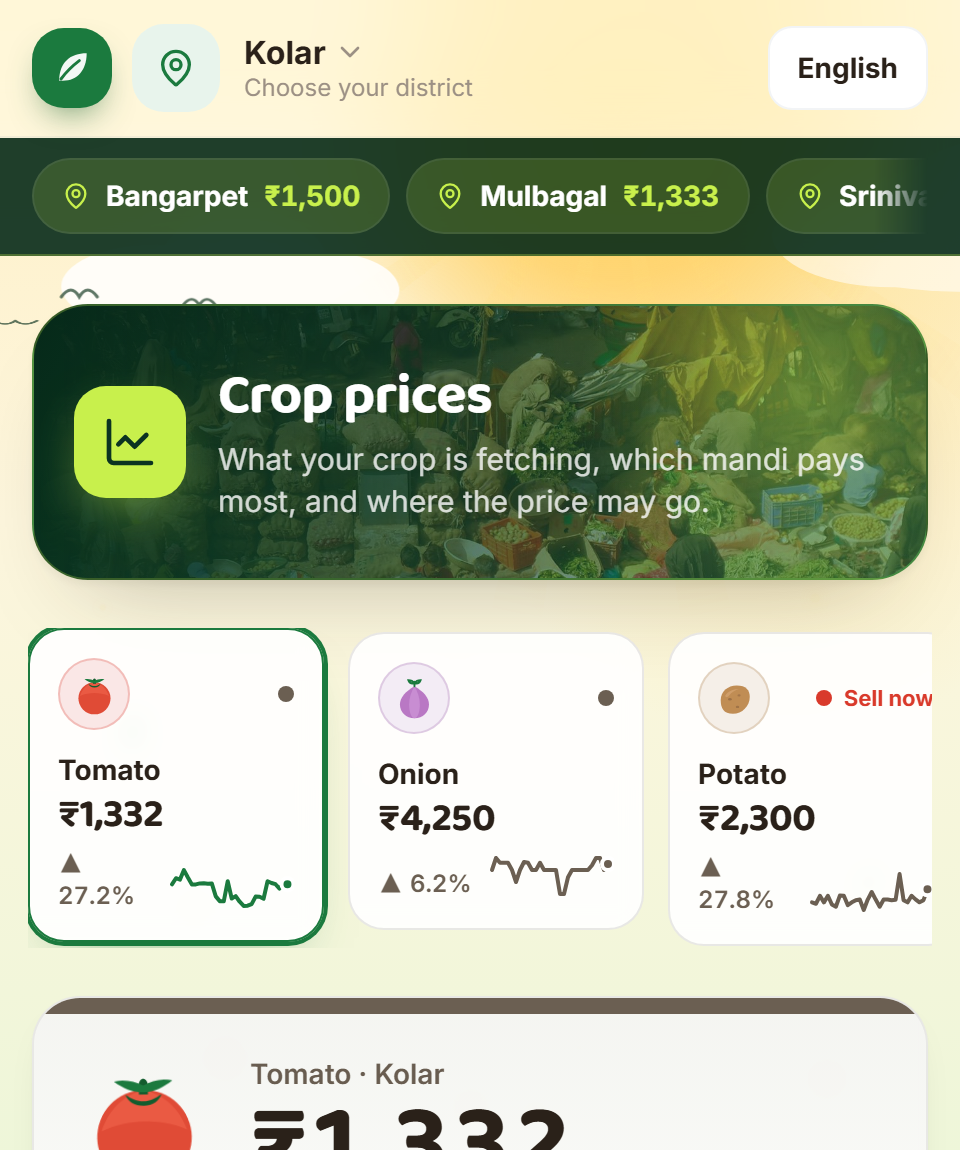
\includegraphics[width=0.94\linewidth,height=9.0cm,keepaspectratio]{figures/shot_f_prices.png}}\\[1mm]{\footnotesize (b) Prices}\end{minipage}
\medskip
\centering \begin{minipage}[t]{0.485\textwidth}\centering\fbox{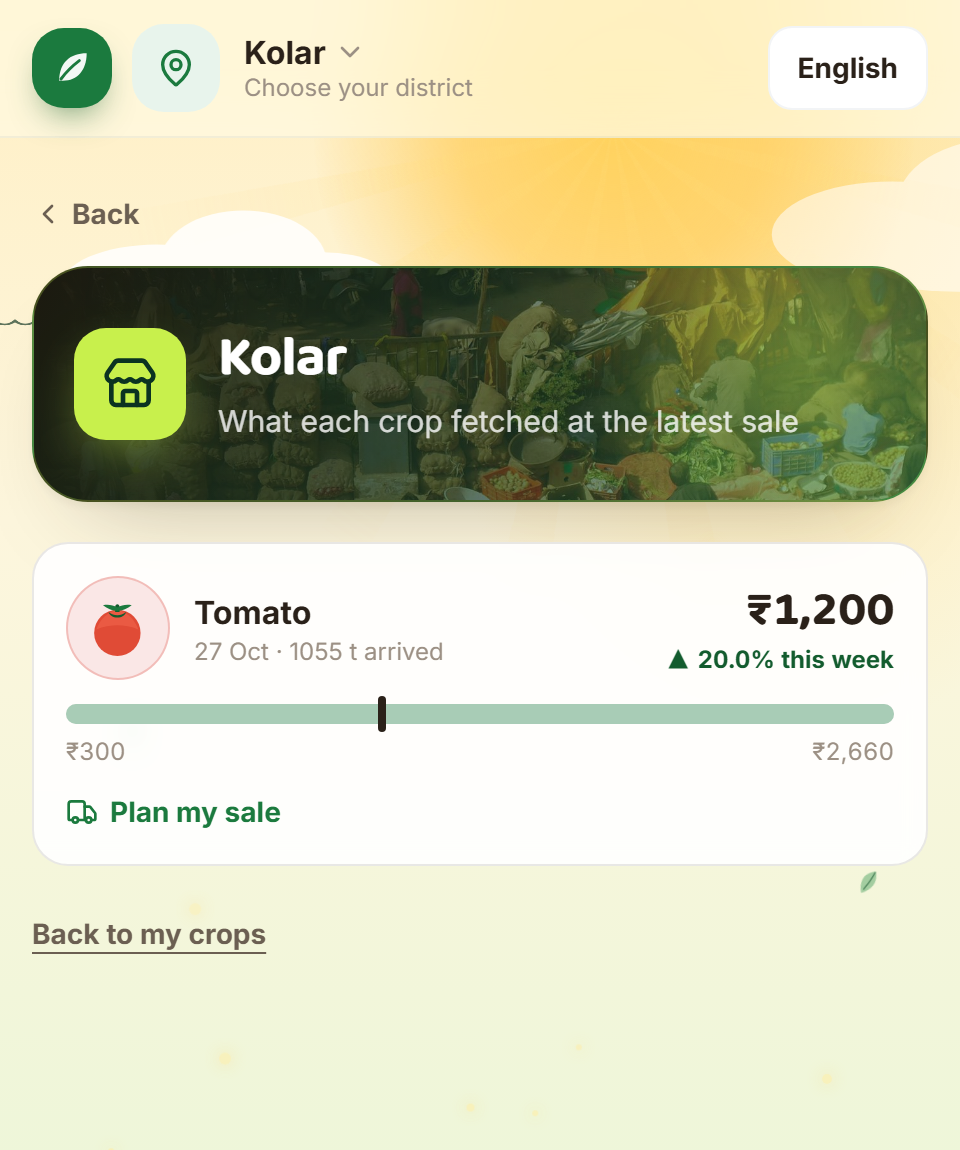
\includegraphics[width=0.94\linewidth,height=9.0cm,keepaspectratio]{figures/shot_f_mandi.png}}\\[1mm]{\footnotesize (c) One mandi}\end{minipage}
\caption{Farmer pages. (a) The home page opens with a plain question, a search box that answers in sentences, and a ticker of the latest prices. (b) The prices page lists the crops with the latest quote, the change over the week and a sparkline. (c) A mandi page shows what each crop fetched there at the latest sale and how many quintals arrived.}
\label{fig:sc-farmer1}
\end{figure}

The home page (Figure~\ref{fig:sc-farmer1}a) deliberately carries no table: the first thing a farmer sees is the question and a box in which to type one in ordinary words. The prices page (b) shows the quote for each crop together with the date of the last report, so a stale price is never presented as today's. The mandi page (c) is the farmer-side view of one market and links to the plan for selling there.


\begin{figure}[!t]
\centering
\begin{minipage}[t]{0.485\textwidth}\centering\fbox{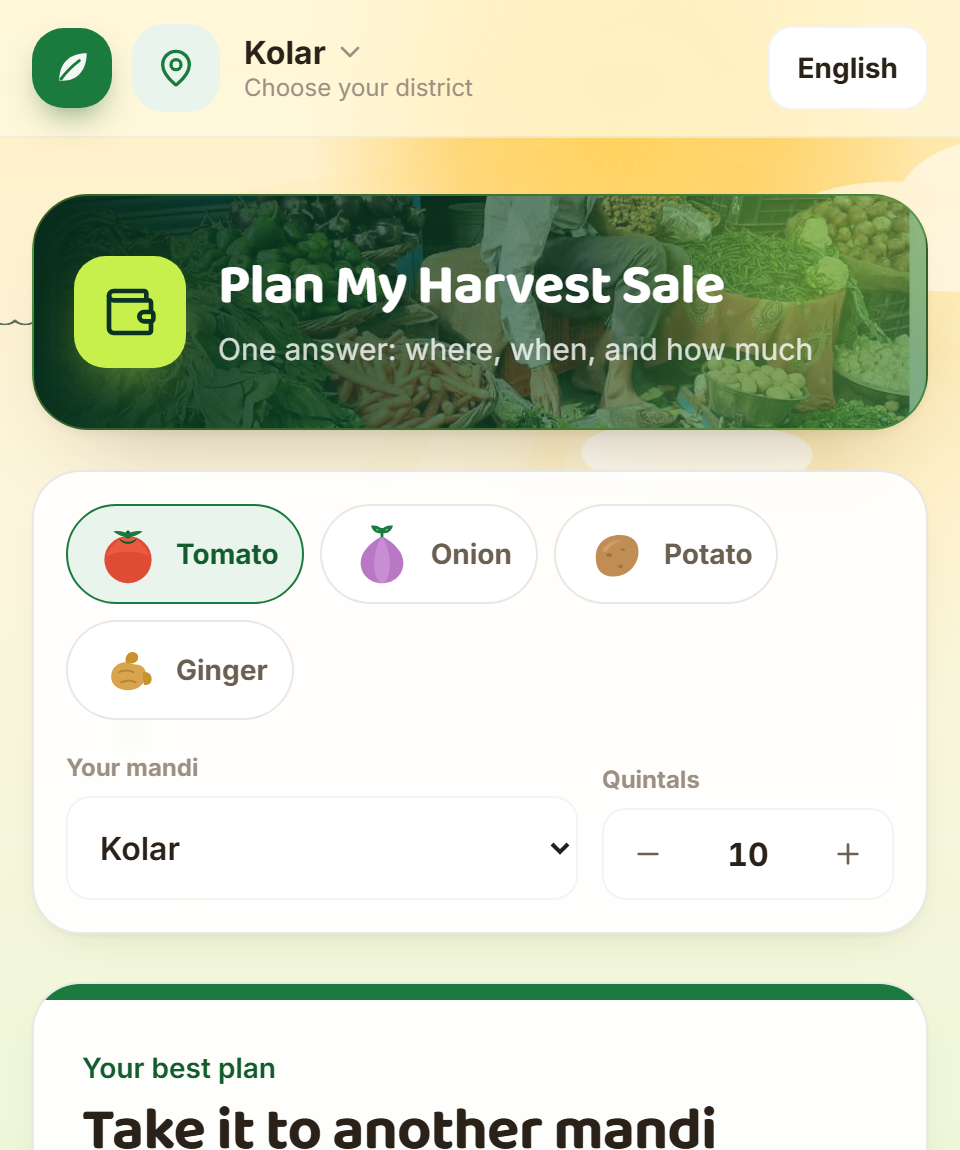
\includegraphics[width=0.94\linewidth,height=9.0cm,keepaspectratio]{figures/shot_f_sellplan.png}}\\[1mm]{\footnotesize (a) Plan my sale}\end{minipage}\hfill
\begin{minipage}[t]{0.485\textwidth}\centering\fbox{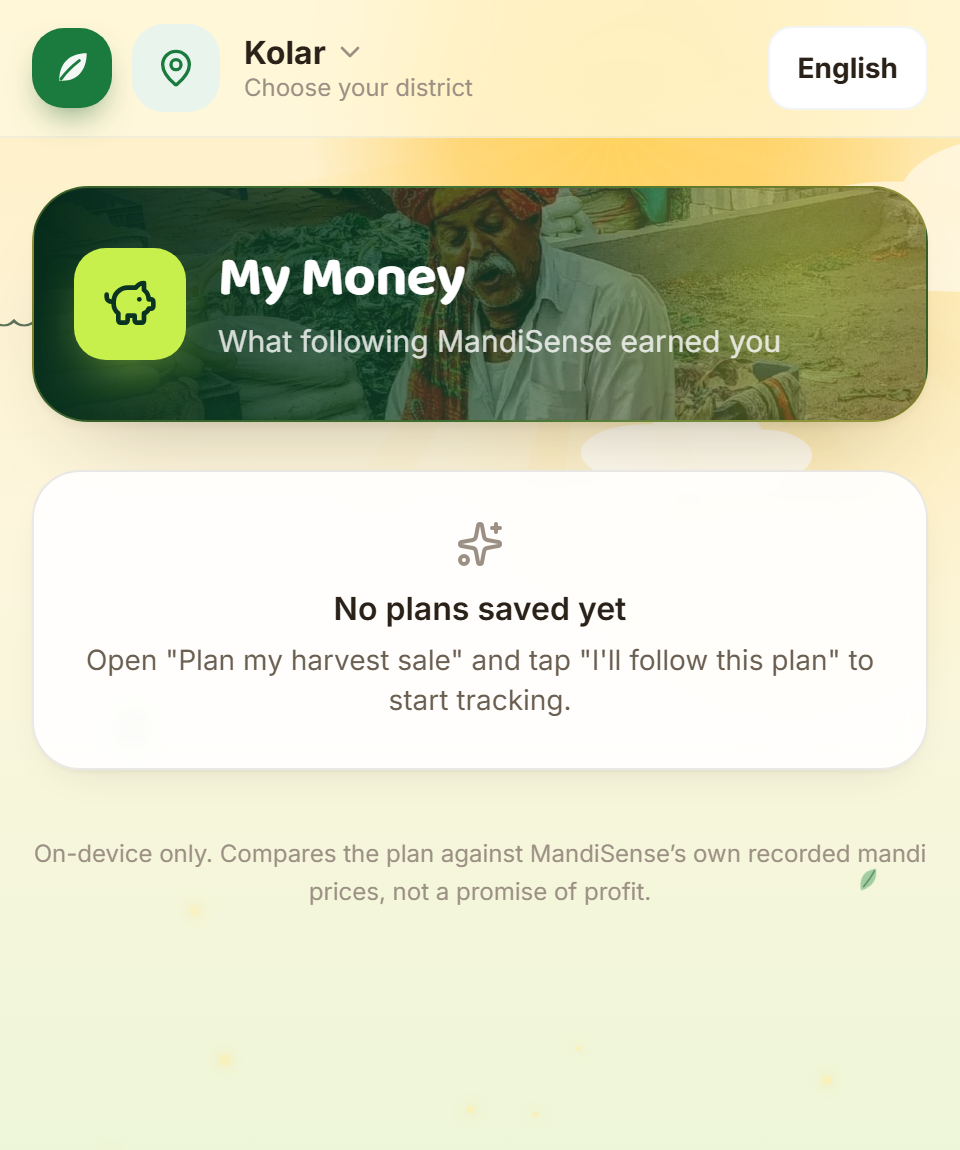
\includegraphics[width=0.94\linewidth,height=9.0cm,keepaspectratio]{figures/shot_f_mymoney.png}}\\[1mm]{\footnotesize (b) My money}\end{minipage}
\medskip
\centering \begin{minipage}[t]{0.485\textwidth}\centering\fbox{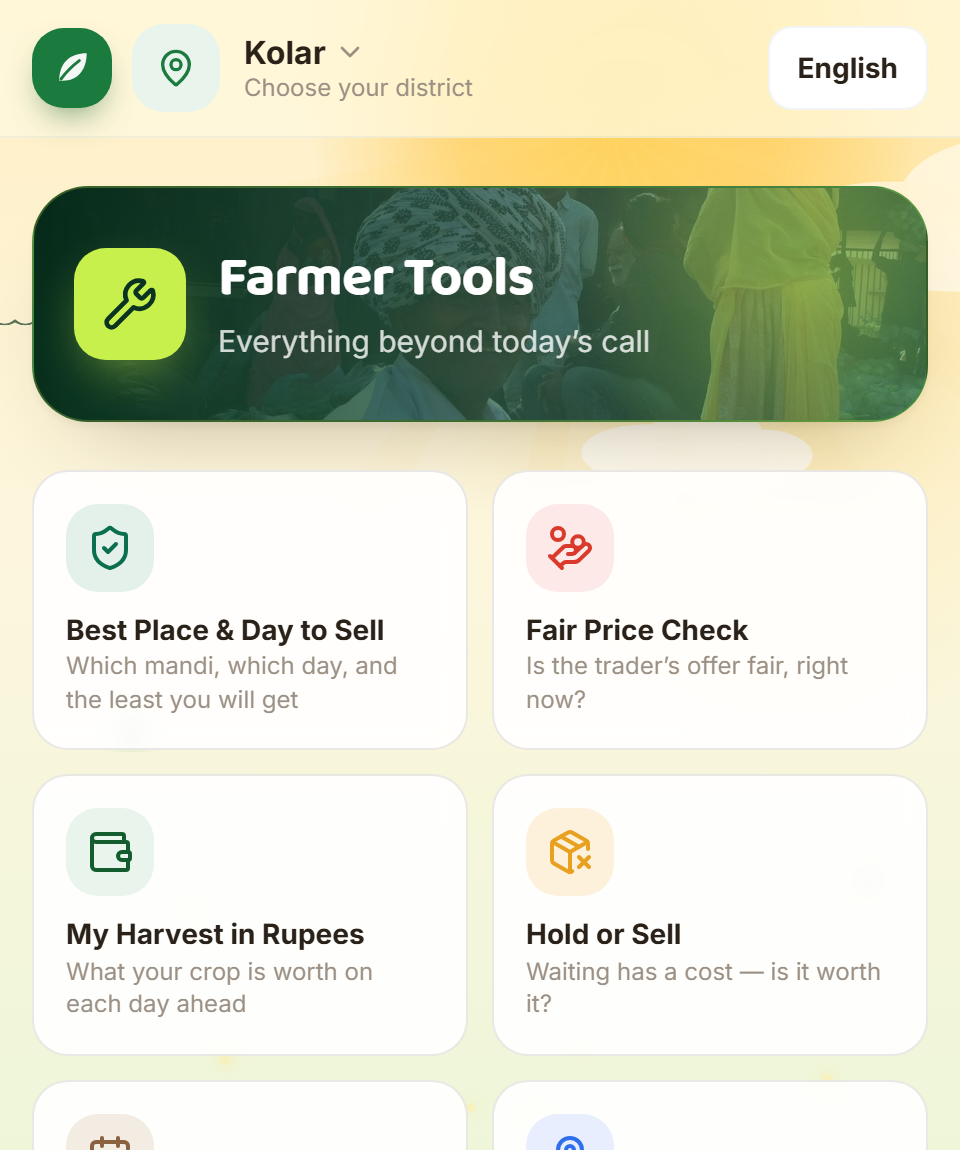
\includegraphics[width=0.94\linewidth,height=9.0cm,keepaspectratio]{figures/shot_f_tools.png}}\\[1mm]{\footnotesize (c) Farmer tools}\end{minipage}
\caption{(a) The sale plan states one recommendation, the amount expected after transport and spoilage, and the day to go. (b) ``My Money'' compares the plans the farmer followed with what the markets recorded; it works on the device only. (c) The tool launcher opens each tool as a sheet over the page.}
\label{fig:sc-farmer2}
\end{figure}

The sale plan (Figure~\ref{fig:sc-farmer2}a) is the product's central screen. It names one market and one day, shows the amount expected per quintal after the cost of moving the crop, and shows the figure the farmer \emph{can count on at least}, which is the revenue floor of Section~\ref{sec:floors}. ``My Money'' (b) keeps the plans on the farmer's phone, so no account or personal data reach the server. The launcher (c) lists the eleven tools whose screens follow.


\begin{figure}[!t]
\centering
\begin{minipage}[t]{0.485\textwidth}\centering\fbox{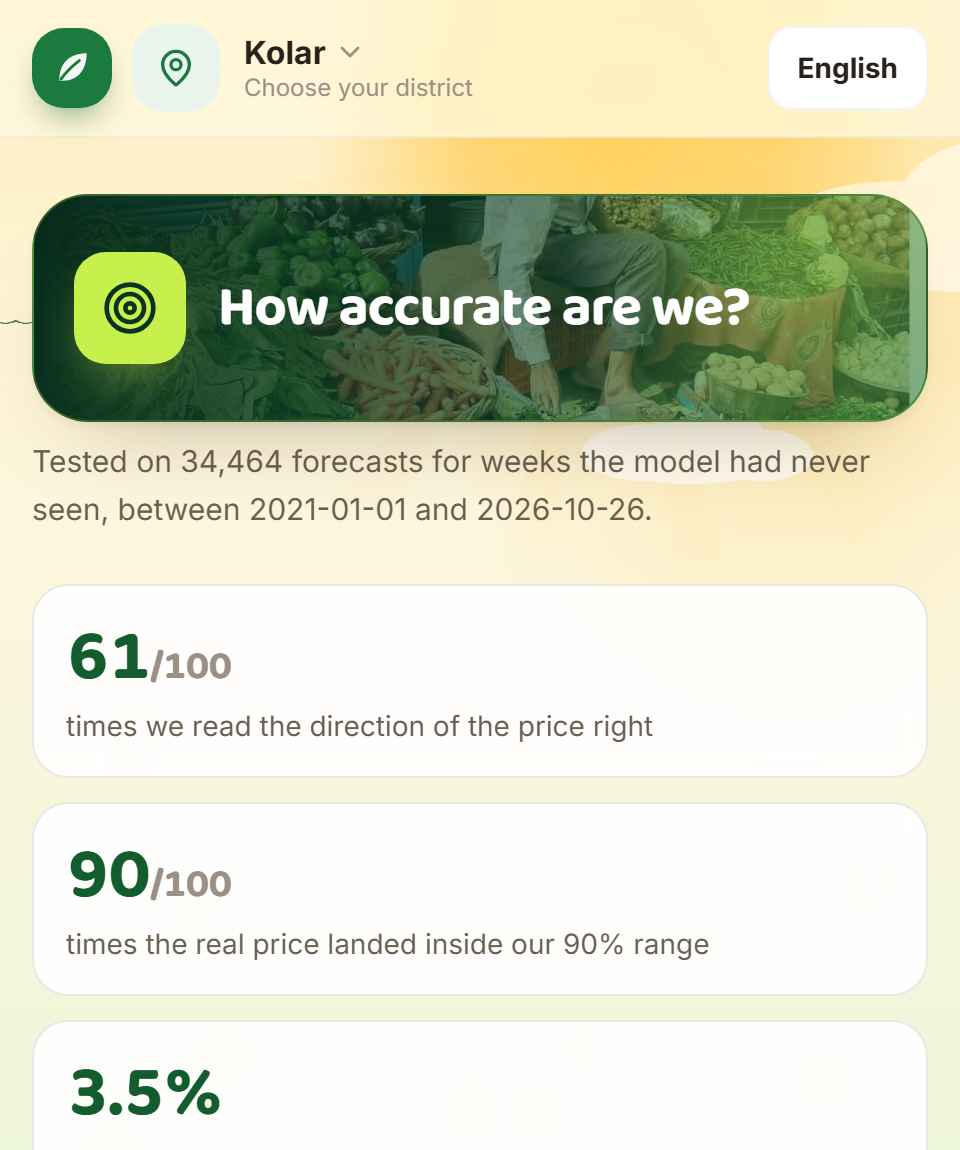
\includegraphics[width=0.94\linewidth,height=9.0cm,keepaspectratio]{figures/shot_f_accuracy.png}}\\[1mm]{\footnotesize (a) How accurate are we?}\end{minipage}\hfill
\begin{minipage}[t]{0.485\textwidth}\centering\fbox{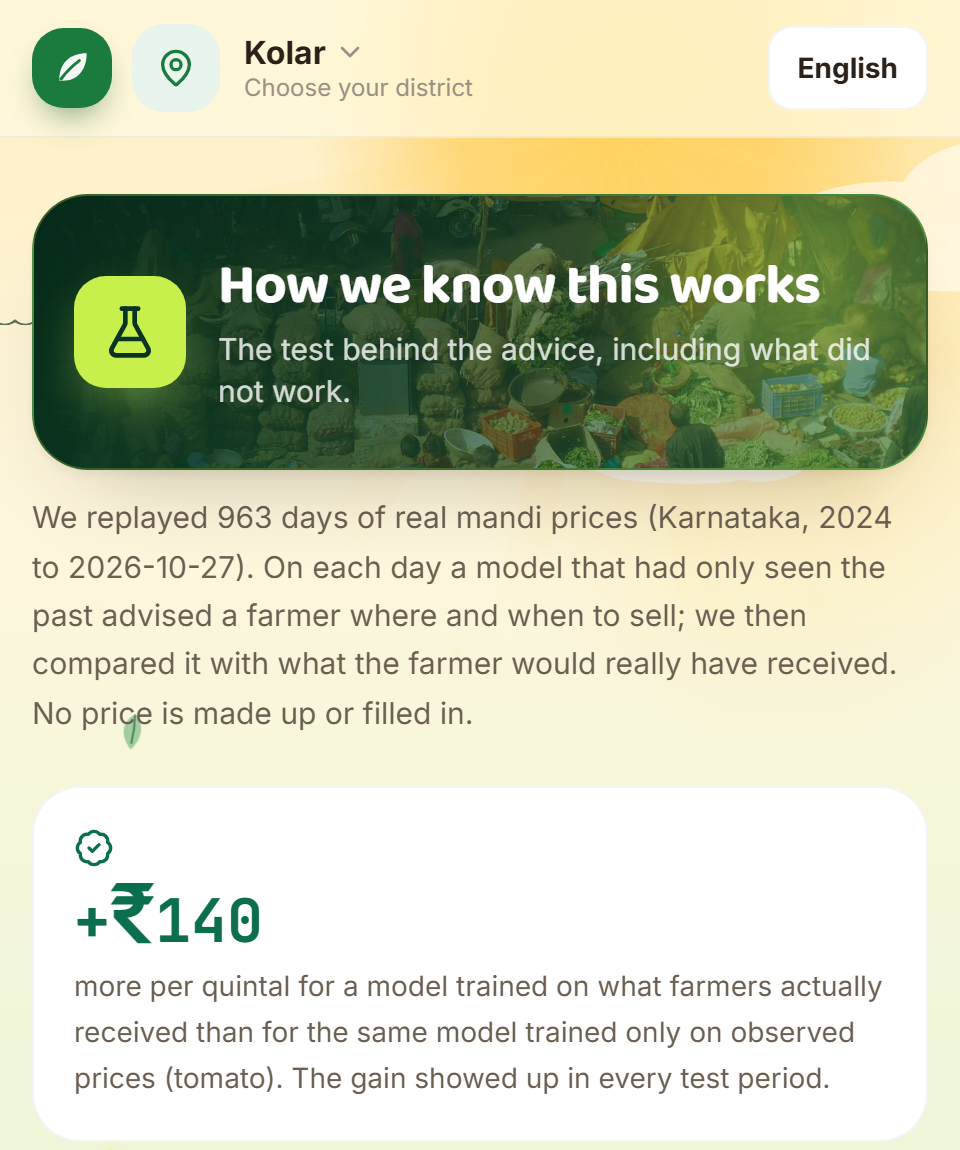
\includegraphics[width=0.94\linewidth,height=9.0cm,keepaspectratio]{figures/shot_f_evidence.png}}\\[1mm]{\footnotesize (b) How we know this works}\end{minipage}
\medskip
\centering \begin{minipage}[t]{0.485\textwidth}\centering\fbox{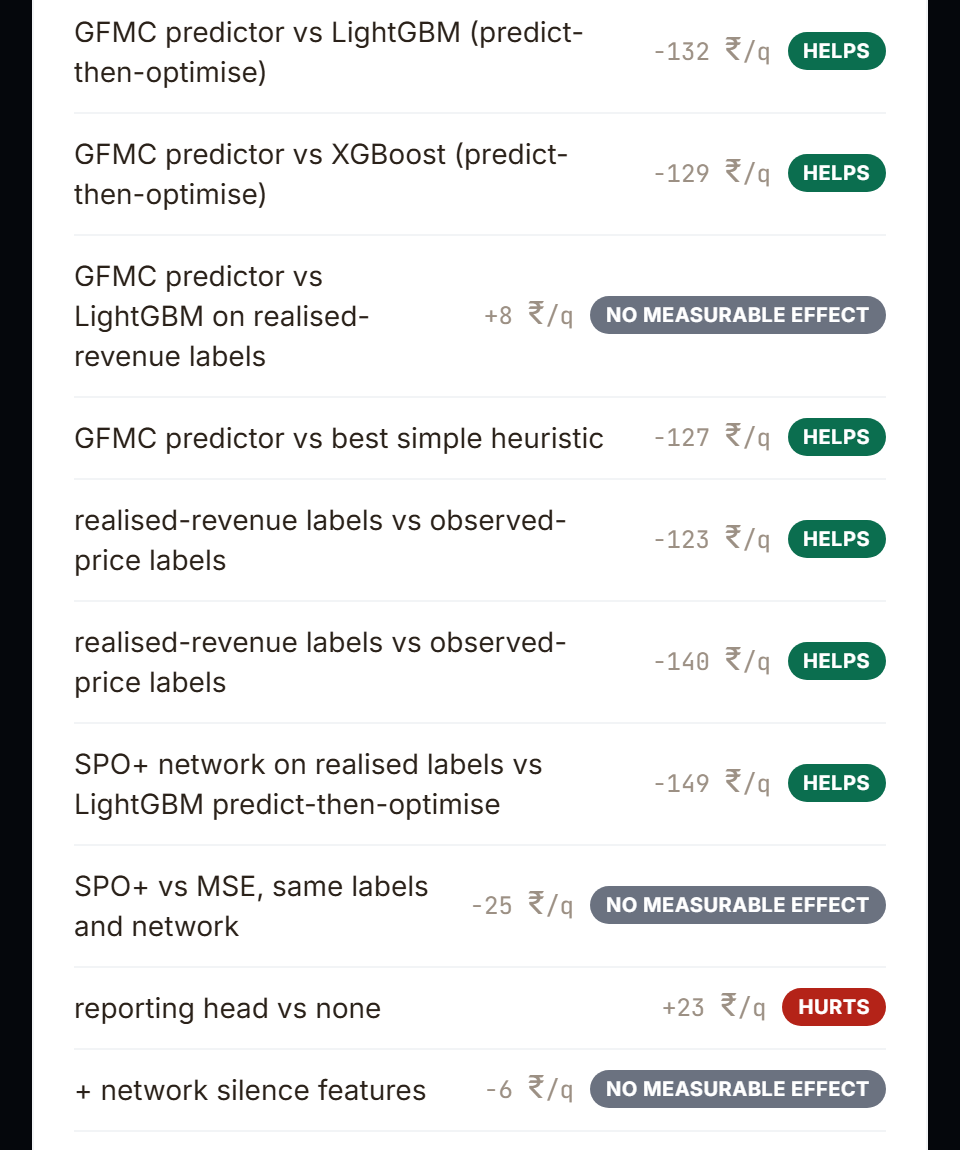
\includegraphics[width=0.94\linewidth,height=9.0cm,keepaspectratio]{figures/shot_f_evidence_b.png}}\\[1mm]{\footnotesize (c) What did not work}\end{minipage}
\caption{The honesty pages. (a) Hit rates by crop and market, on days the system had not seen. (b) The replay: what the method earns against simple alternatives, in rupees, with the seed-to-seed spread. (c) The negative results are listed beside the positive ones.}
\label{fig:sc-farmer3}
\end{figure}

Three pages exist only to let a reader check the system. The accuracy page (Figure~\ref{fig:sc-farmer3}a) reports, per crop and market, how often the advice held on days the system had not seen. The evidence page (b) reproduces the main comparison of Chapter~\ref{ch:results} in plain words and in rupees, and (c) lists what did not help. A product that shows its misses is easier to trust than one that does not.

\subsection{Farmer tools}
Each tool opens as a sheet over the page and answers one question. The sheets below are captured with the sheet in its resting state; the blurred page behind each sheet is cropped away.


\begin{figure}[!t]
\centering
\begin{minipage}[t]{0.485\textwidth}\centering\fbox{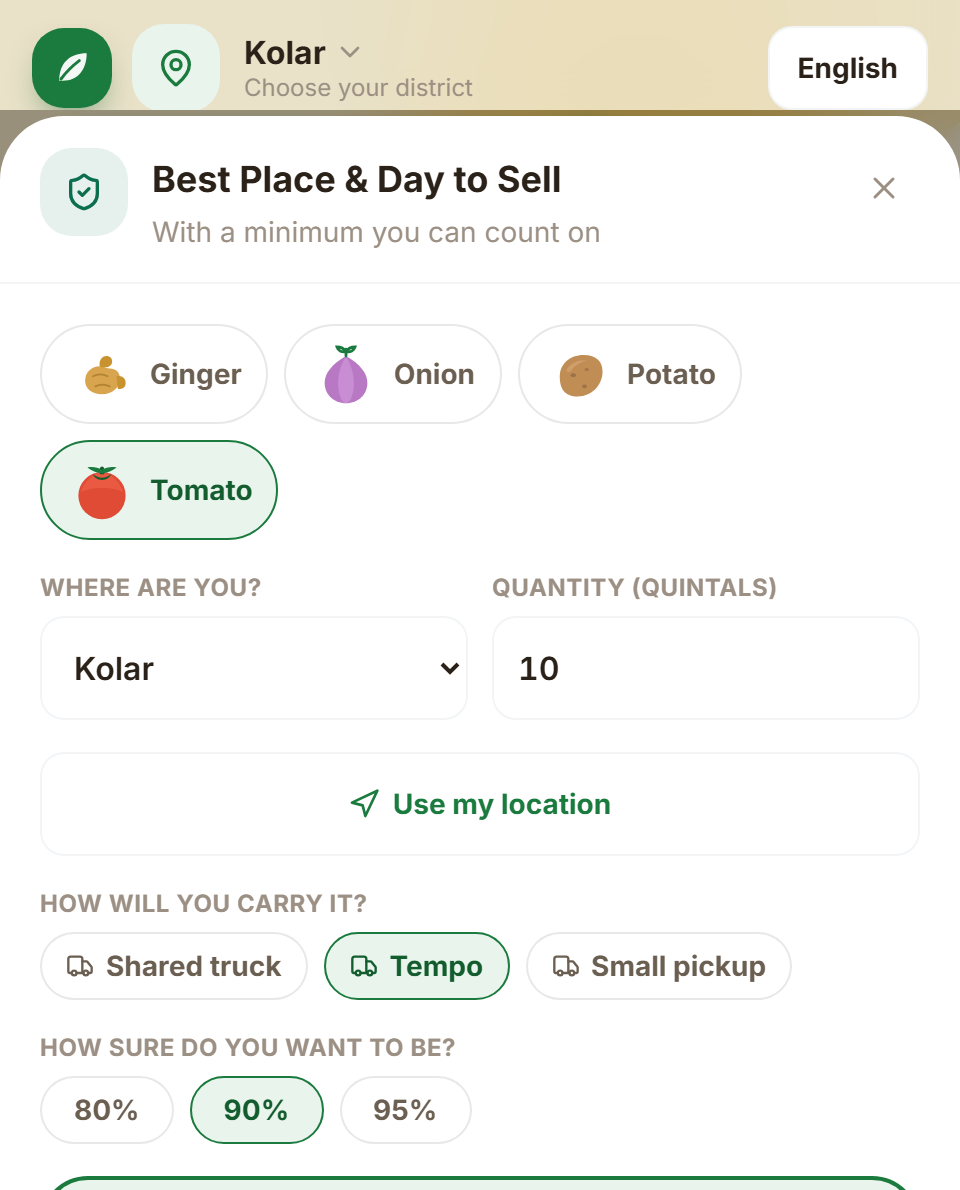
\includegraphics[width=0.94\linewidth,height=9.0cm,keepaspectratio]{figures/shot_t_besplace.png}}\\[1mm]{\footnotesize (a) Best place and day}\end{minipage}\hfill
\begin{minipage}[t]{0.485\textwidth}\centering\fbox{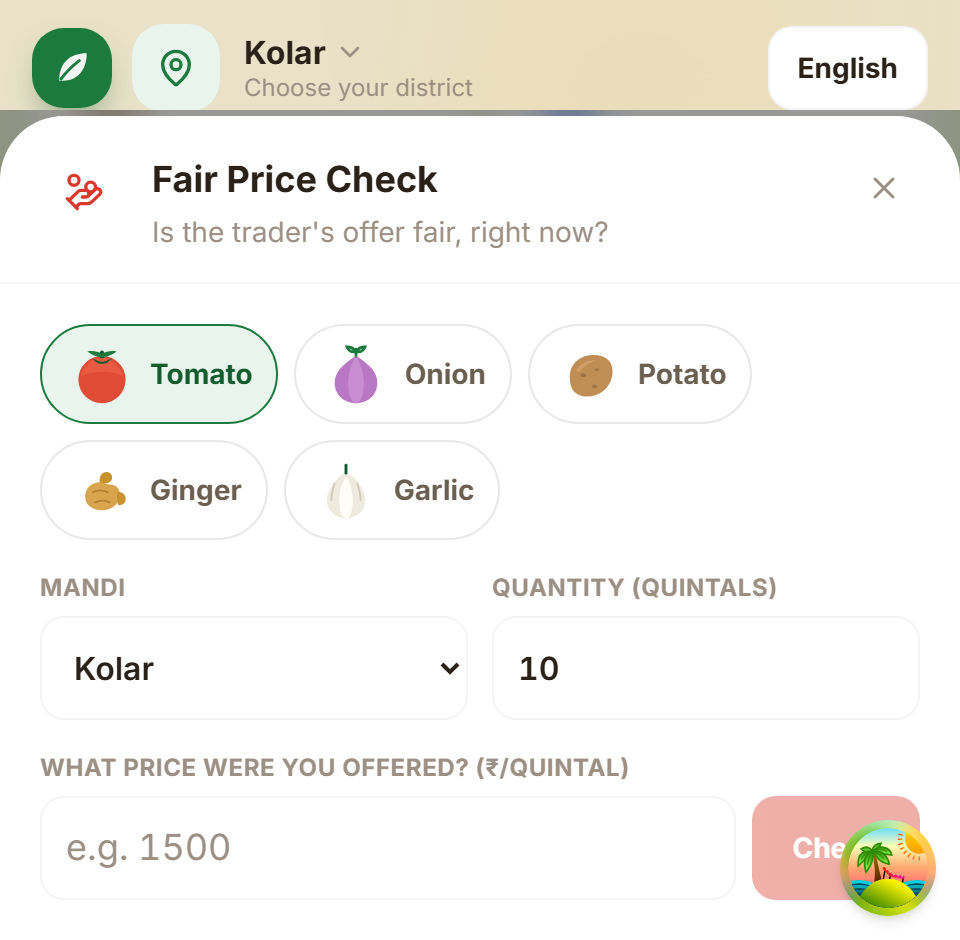
\includegraphics[width=0.94\linewidth,height=9.0cm,keepaspectratio]{figures/shot_t_fairprice.png}}\\[1mm]{\footnotesize (b) Fair price check}\end{minipage}
\medskip
\centering \begin{minipage}[t]{0.485\textwidth}\centering\fbox{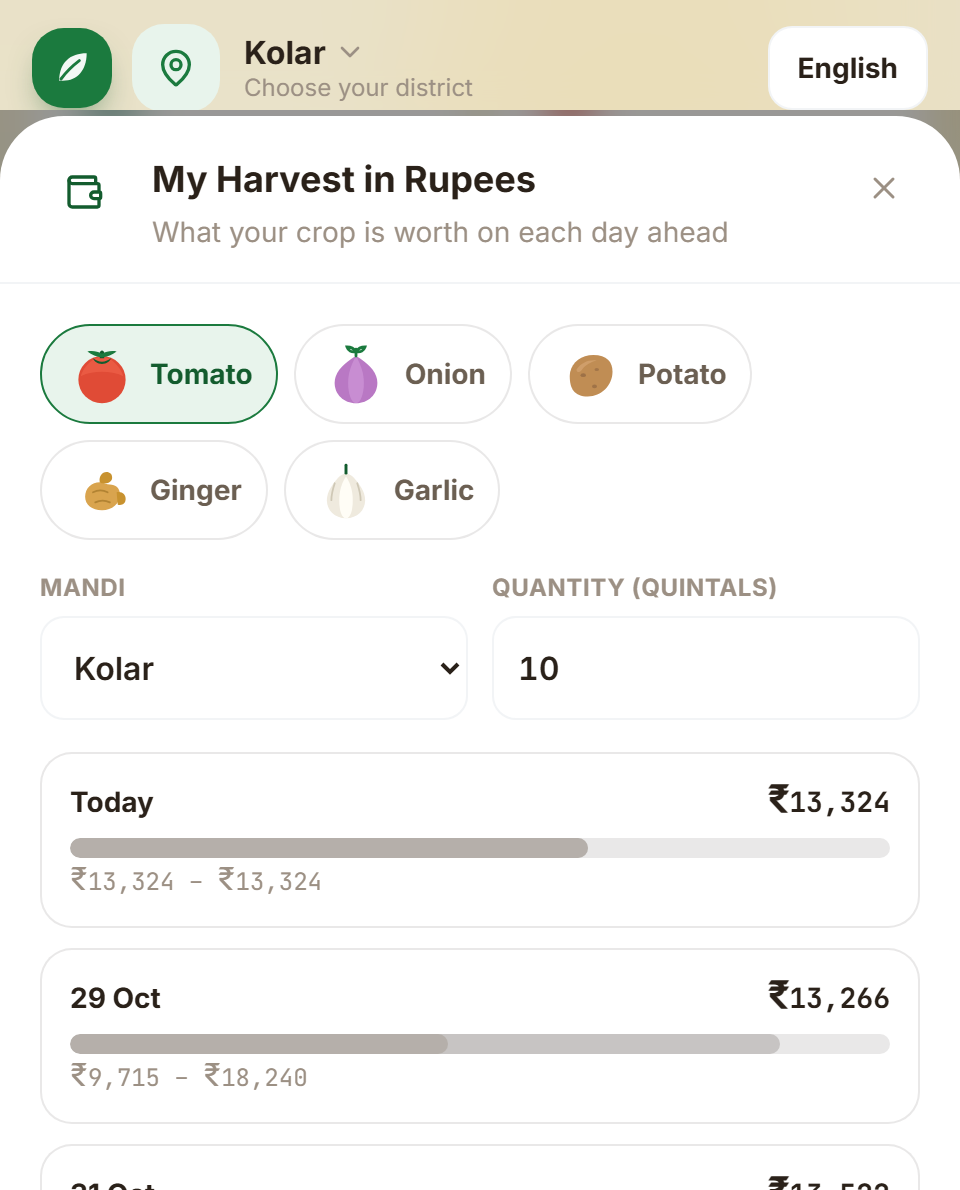
\includegraphics[width=0.94\linewidth,height=9.0cm,keepaspectratio]{figures/shot_t_harvest.png}}\\[1mm]{\footnotesize (c) My harvest in rupees}\end{minipage}
\caption{Selling tools. (a) The recommended market with expected and guaranteed amounts, options to change the vehicle and the confidence, and the next best choices. (b) A check of whether the price a trader offered is fair. (c) The expected value of the crop on each day ahead, after spoilage.}
\label{fig:sc-tools1}
\end{figure}

The Best Place and Day to Sell sheet (Figure~\ref{fig:sc-tools1}a) asks for the district, the quantity, the vehicle and the confidence level (80, 90 or 95\%), and returns the same recommendation as the service of Section~\ref{sec:service-app}, with the cost arithmetic one tap away. The fair-price check (b) takes the offer a trader made and places it against the distribution of recent prices. The harvest sheet (c) lays the next days side by side as a bar for each, with the expected net value, so the farmer sees what waiting costs.


\begin{figure}[!t]
\centering
\begin{minipage}[t]{0.485\textwidth}\centering\fbox{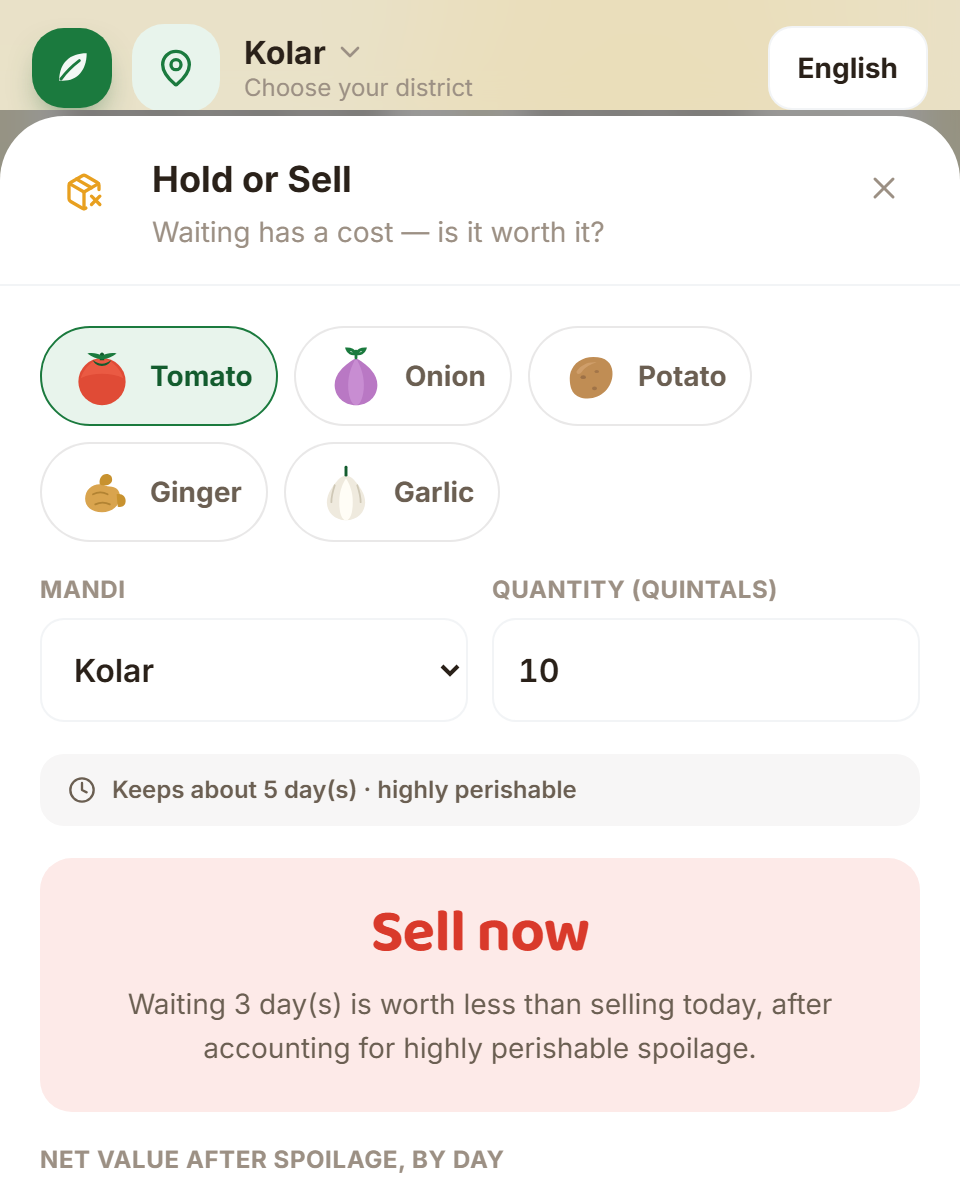
\includegraphics[width=0.94\linewidth,height=9.0cm,keepaspectratio]{figures/shot_t_holdorsell.png}}\\[1mm]{\footnotesize (a) Hold or sell}\end{minipage}\hfill
\begin{minipage}[t]{0.485\textwidth}\centering\fbox{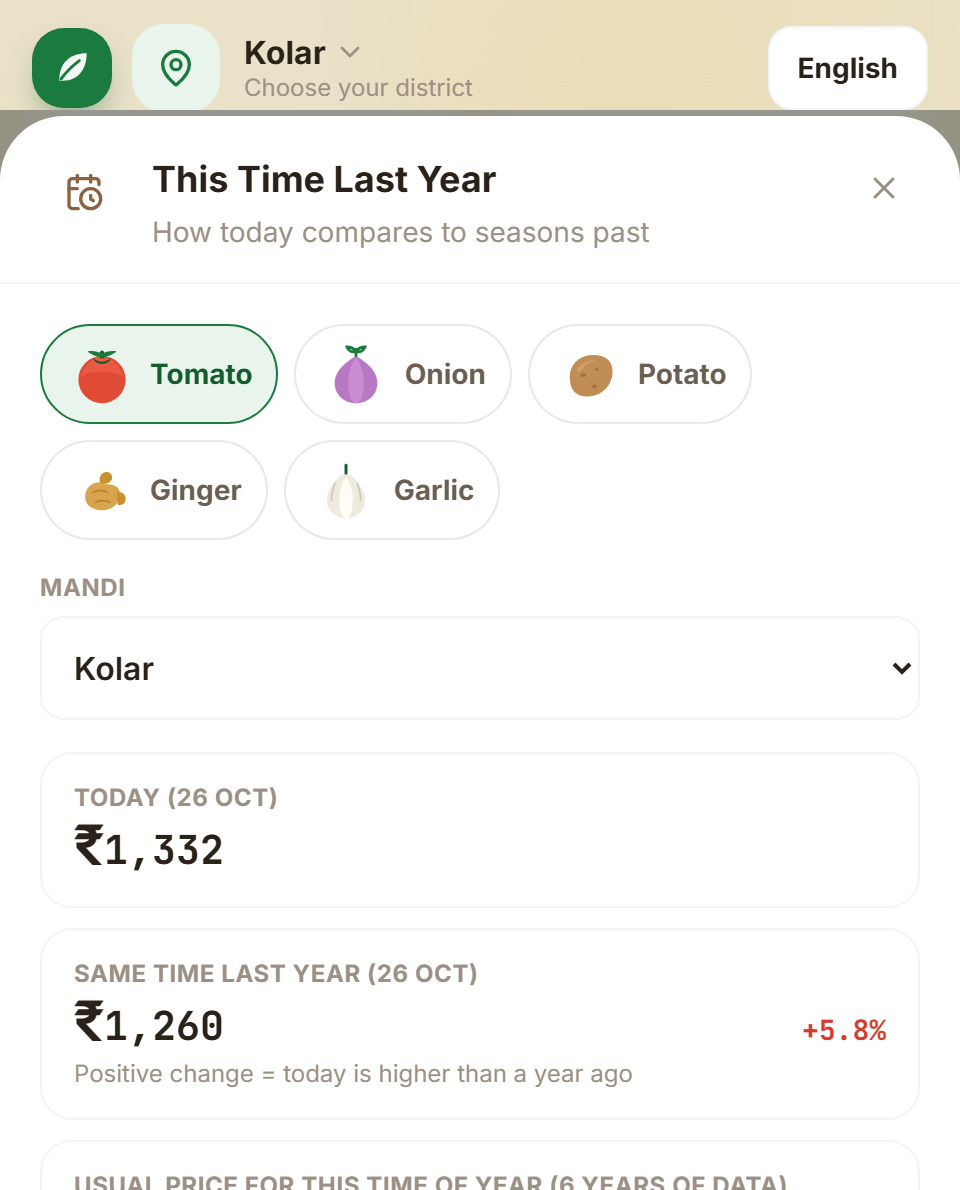
\includegraphics[width=0.94\linewidth,height=9.0cm,keepaspectratio]{figures/shot_t_lastyear.png}}\\[1mm]{\footnotesize (b) This time last year}\end{minipage}
\medskip
\centering \begin{minipage}[t]{0.485\textwidth}\centering\fbox{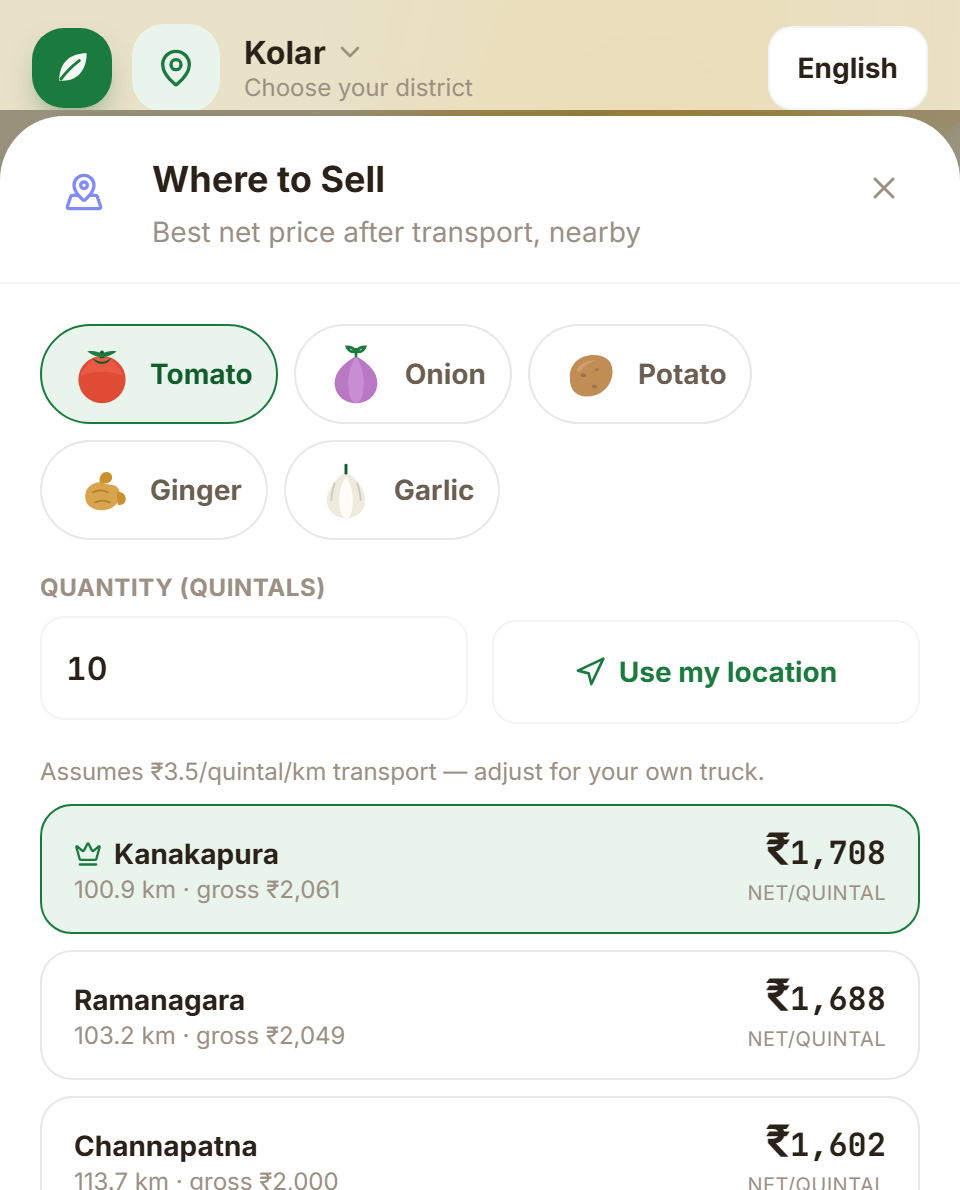
\includegraphics[width=0.94\linewidth,height=9.0cm,keepaspectratio]{figures/shot_t_wheretosell.png}}\\[1mm]{\footnotesize (c) Where to sell}\end{minipage}
\caption{Timing and location tools. (a) A hold-or-sell call that weighs spoilage against the expected price gain. (b) Today's price against the same date last year and the seasonal norm. (c) Nearby markets ranked by price after transport.}
\label{fig:sc-tools2}
\end{figure}

Hold or Sell (Figure~\ref{fig:sc-tools2}a) is built for the perishable case: it states the cost of waiting a day, so that ``wait'' is never the free option it appears to be. The seasonal sheet (b) gives context, not a forecast, and is labelled so. The ranking (c) lists markets with distance, gross price and net price per quintal under an assumed transport cost that the farmer can change.


\begin{figure}[!t]
\centering
\begin{minipage}[t]{0.485\textwidth}\centering\fbox{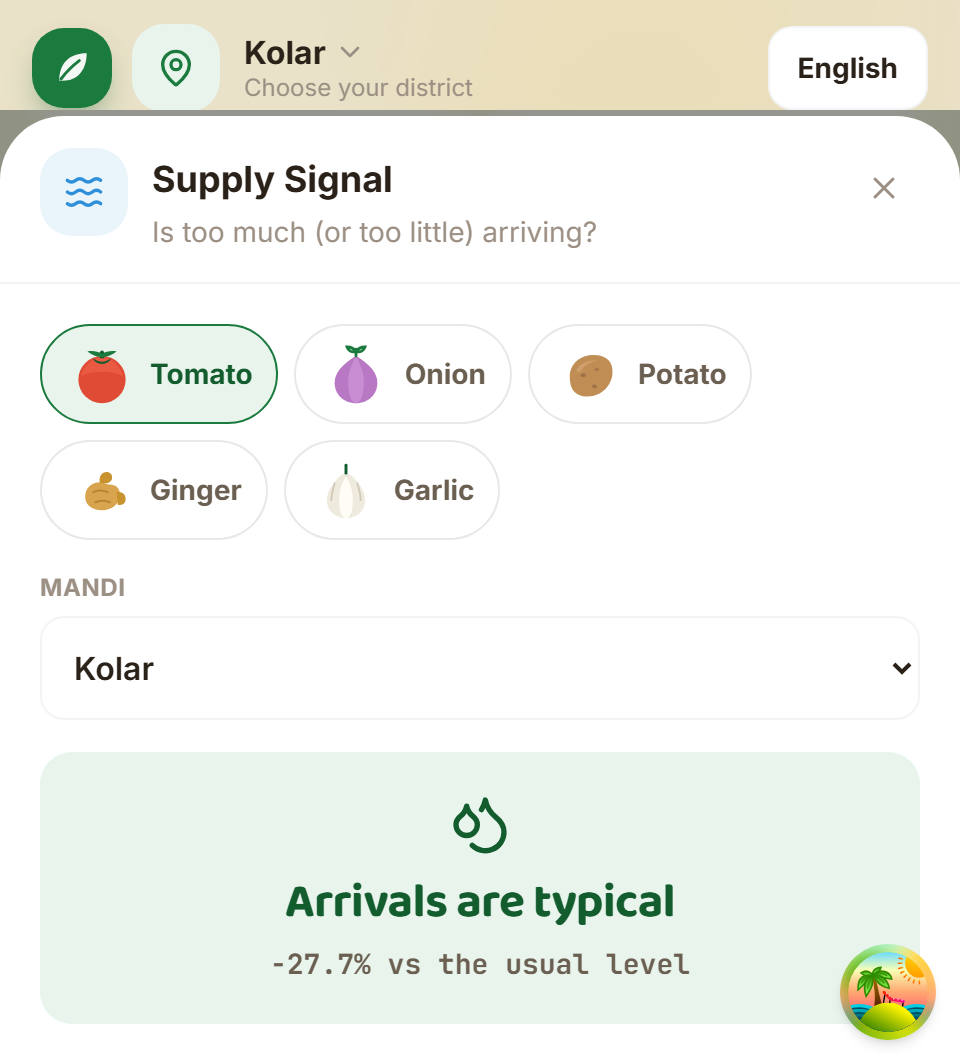
\includegraphics[width=0.94\linewidth,height=9.0cm,keepaspectratio]{figures/shot_t_supply.png}}\\[1mm]{\footnotesize (a) Supply signal}\end{minipage}\hfill
\begin{minipage}[t]{0.485\textwidth}\centering\fbox{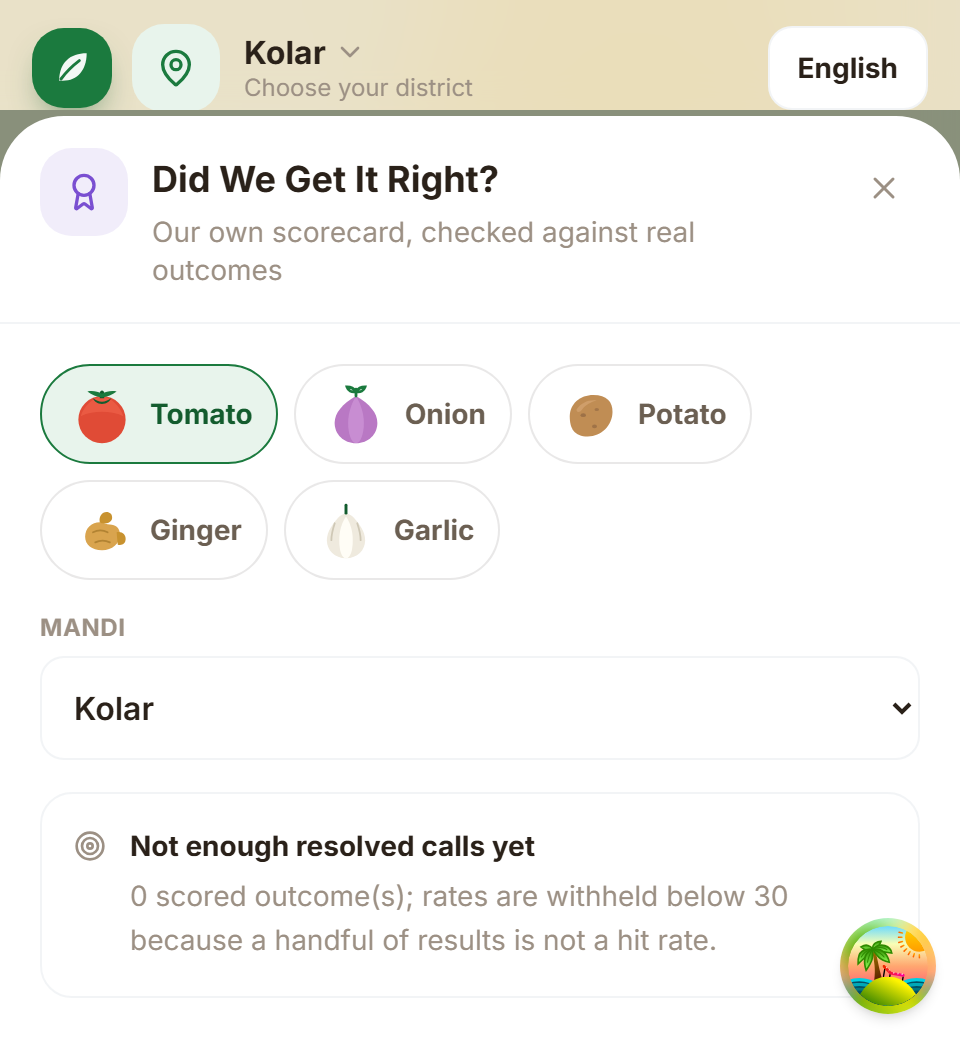
\includegraphics[width=0.94\linewidth,height=9.0cm,keepaspectratio]{figures/shot_t_record.png}}\\[1mm]{\footnotesize (b) Did we get it right?}\end{minipage}
\medskip
\centering \begin{minipage}[t]{0.485\textwidth}\centering\fbox{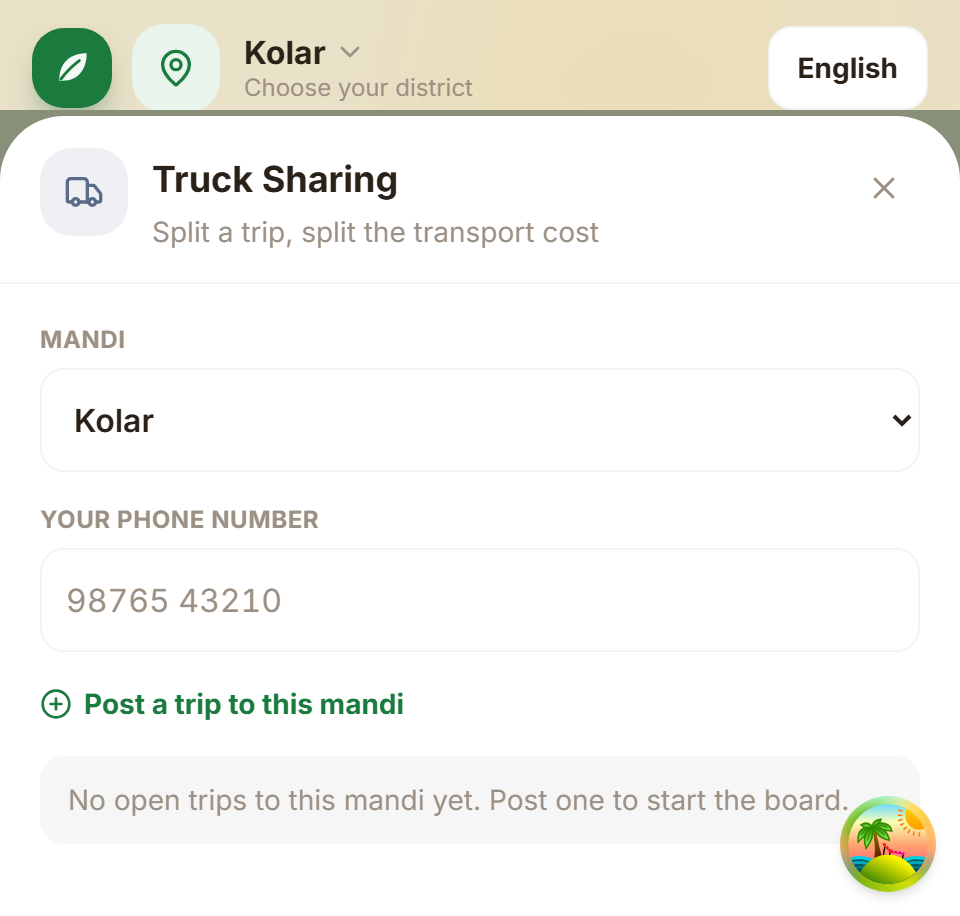
\includegraphics[width=0.94\linewidth,height=9.0cm,keepaspectratio]{figures/shot_t_truck.png}}\\[1mm]{\footnotesize (c) Truck sharing}\end{minipage}
\caption{Context and sharing tools. (a) Arrivals against the usual level. (b) The system's own scorecard of resolved calls. (c) A board for splitting a truck to a market.}
\label{fig:sc-tools3}
\end{figure}

The supply signal (Figure~\ref{fig:sc-tools3}a) reports whether arrivals are unusually high or low, since a glut lowers price. The scorecard (b) is an honest counter: when too few calls have resolved it says so and withholds the rate. The truck-sharing board (c) is a prototype that lets a farmer post a trip so that others can share the transport cost.


\begin{figure}[!t]
\centering
\begin{minipage}[t]{0.485\textwidth}\centering\fbox{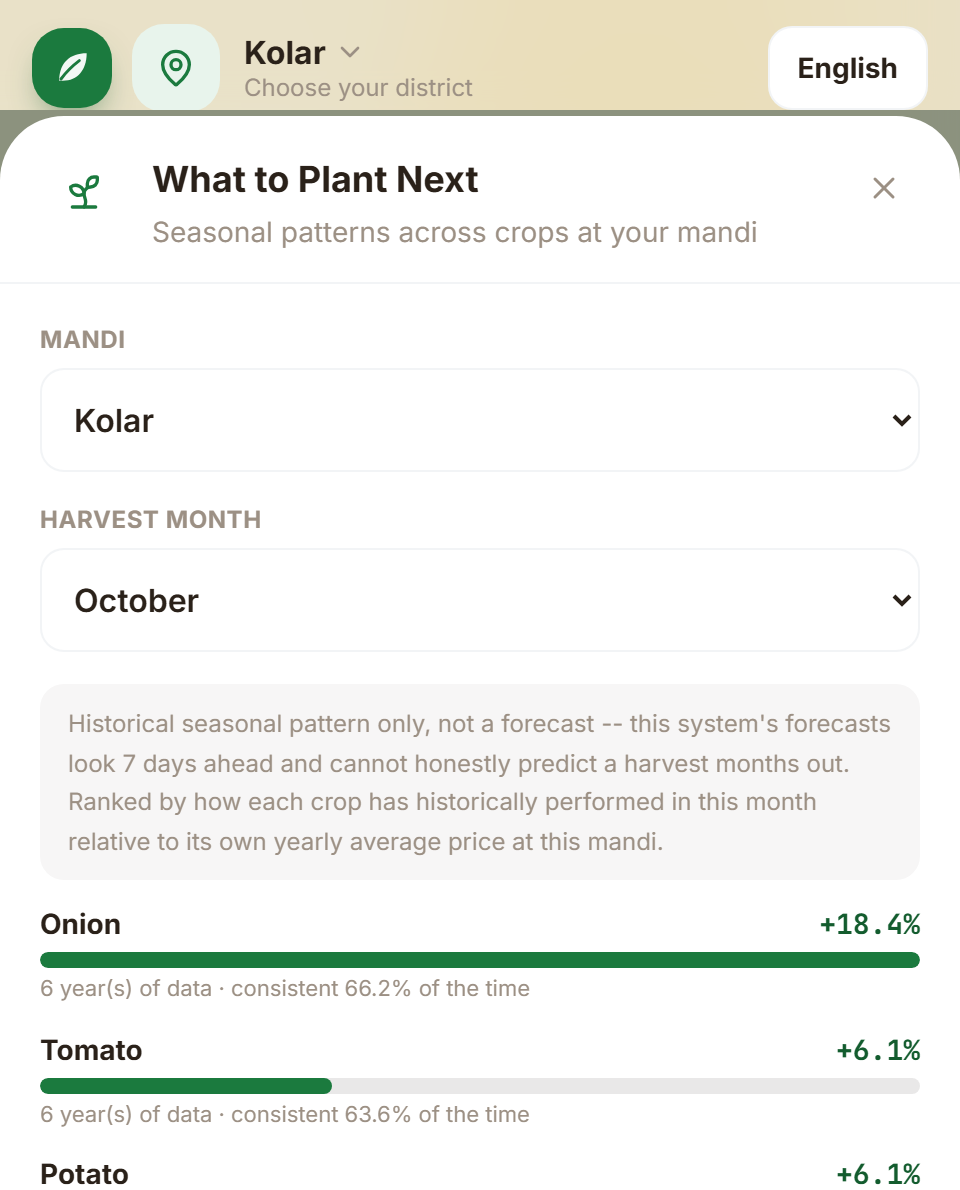
\includegraphics[width=0.94\linewidth,height=9.0cm,keepaspectratio]{figures/shot_t_plant.png}}\\[1mm]{\footnotesize (a) What to plant next}\end{minipage}\hfill
\begin{minipage}[t]{0.485\textwidth}\centering\fbox{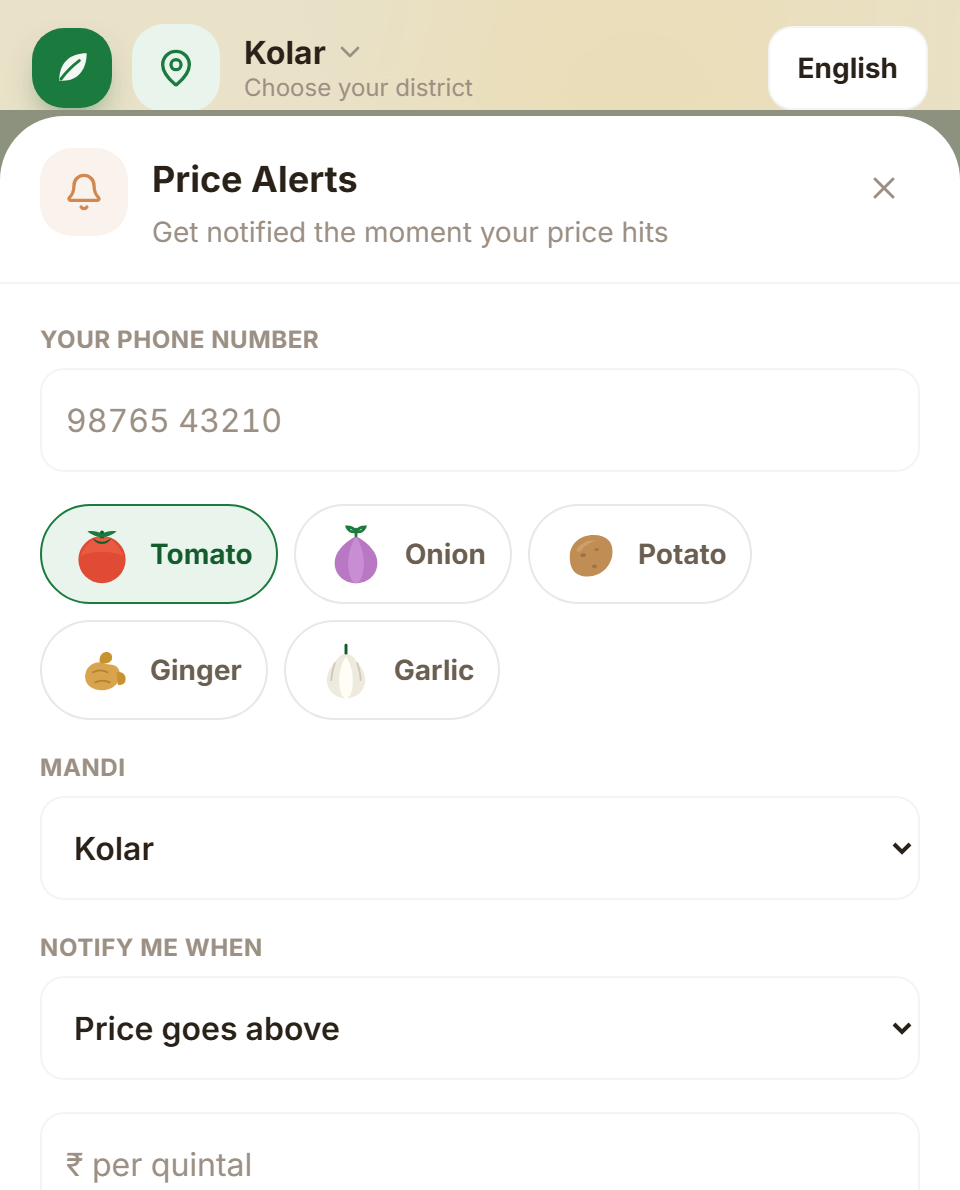
\includegraphics[width=0.94\linewidth,height=9.0cm,keepaspectratio]{figures/shot_t_alerts.png}}\\[1mm]{\footnotesize (b) Price alerts}\end{minipage}
\caption{(a) Seasonal patterns by crop for a chosen harvest month, from past years. (b) A price alert that notifies the farmer when a crop reaches a chosen price.}
\label{fig:sc-tools4}
\end{figure}

What to Plant Next (Figure~\ref{fig:sc-tools4}a) is explicitly historical: it shows how each crop has behaved in the chosen month in previous years and does not forecast the coming season. The alert sheet (b) is the entry point for the Telegram digest of Section~\ref{sec:digest-method}.


\subsection{Advice that can be checked}
The three panels of Figure~\ref{fig:ui-insight} (Section~\ref{sec:insight-method}) sit inside the Best Place sheet. They show the arithmetic behind the choice, what changes if the farmer's costs differ, and how the advice would have done on days it had not seen. The morning digest of Section~\ref{sec:digest-method} is the same advice delivered as a message.

\subsection{Trader desk}
The trader desk is a set of analytical tools for buyers and for the project's own examination of its method. It is laid out for a wide screen.

\begin{figure}[!t]
\centering
\fbox{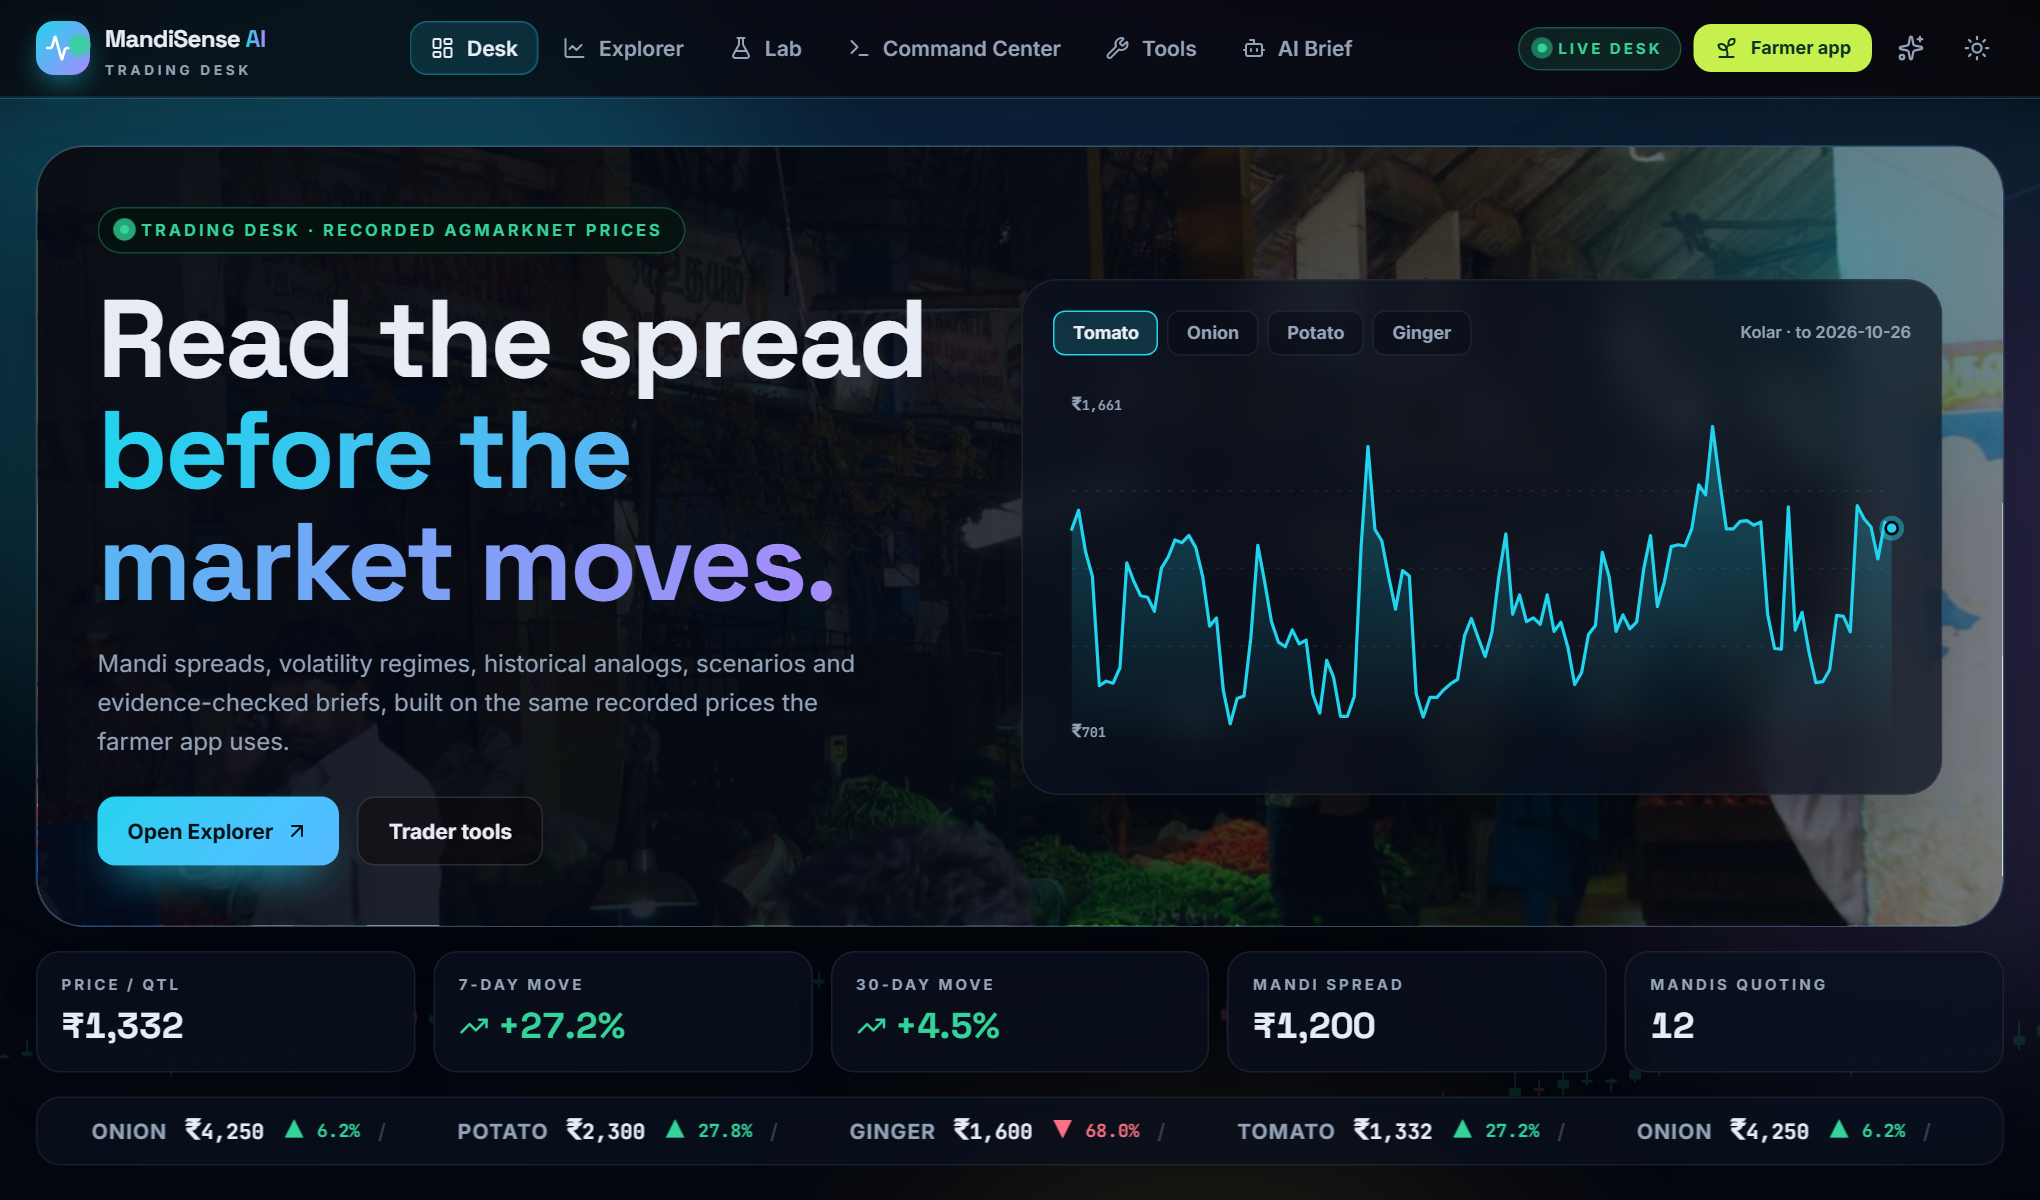
\includegraphics[width=0.93\linewidth]{figures/shot_w_trader.png}}\\[0.5mm]{\footnotesize (a) Trader home: the day's key signals and entry points to the tools below}
\medskip
\fbox{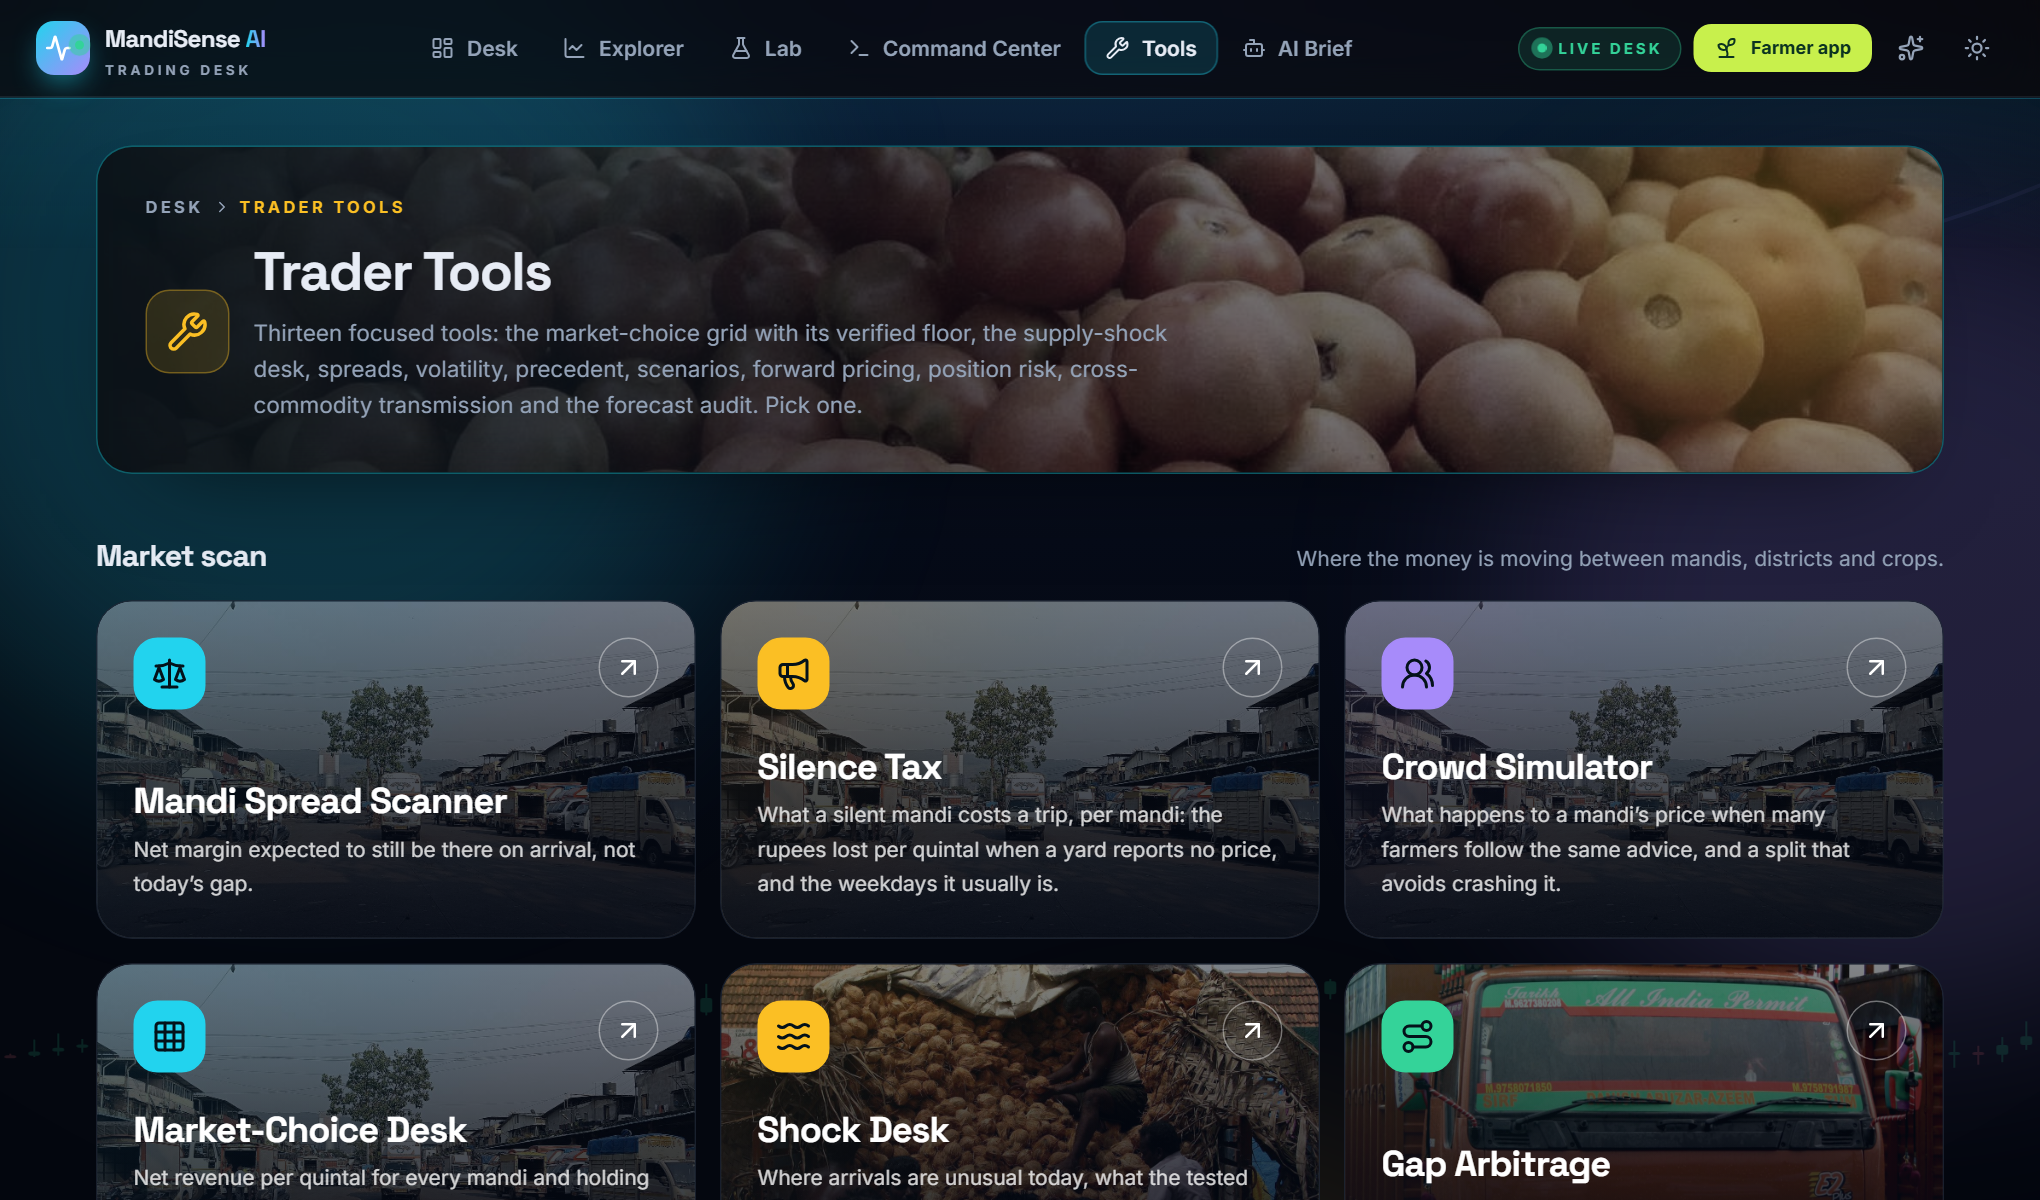
\includegraphics[width=0.93\linewidth]{figures/shot_w_tradertools.png}}\\[0.5mm]{\footnotesize (b) The trader tools index}
\caption{(a) Trader home: the day's key signals and entry points to the tools below. (b) The trader tools index.}
\label{fig:sc-w-trader}
\end{figure}

The trader home page gathers the day's signals, such as the largest price gaps between markets, supply shocks and the status of the advice, and links each to its tool.

The index lists every analytical tool with a one-line statement of the question it answers.

\begin{figure}[!t]
\centering
\fbox{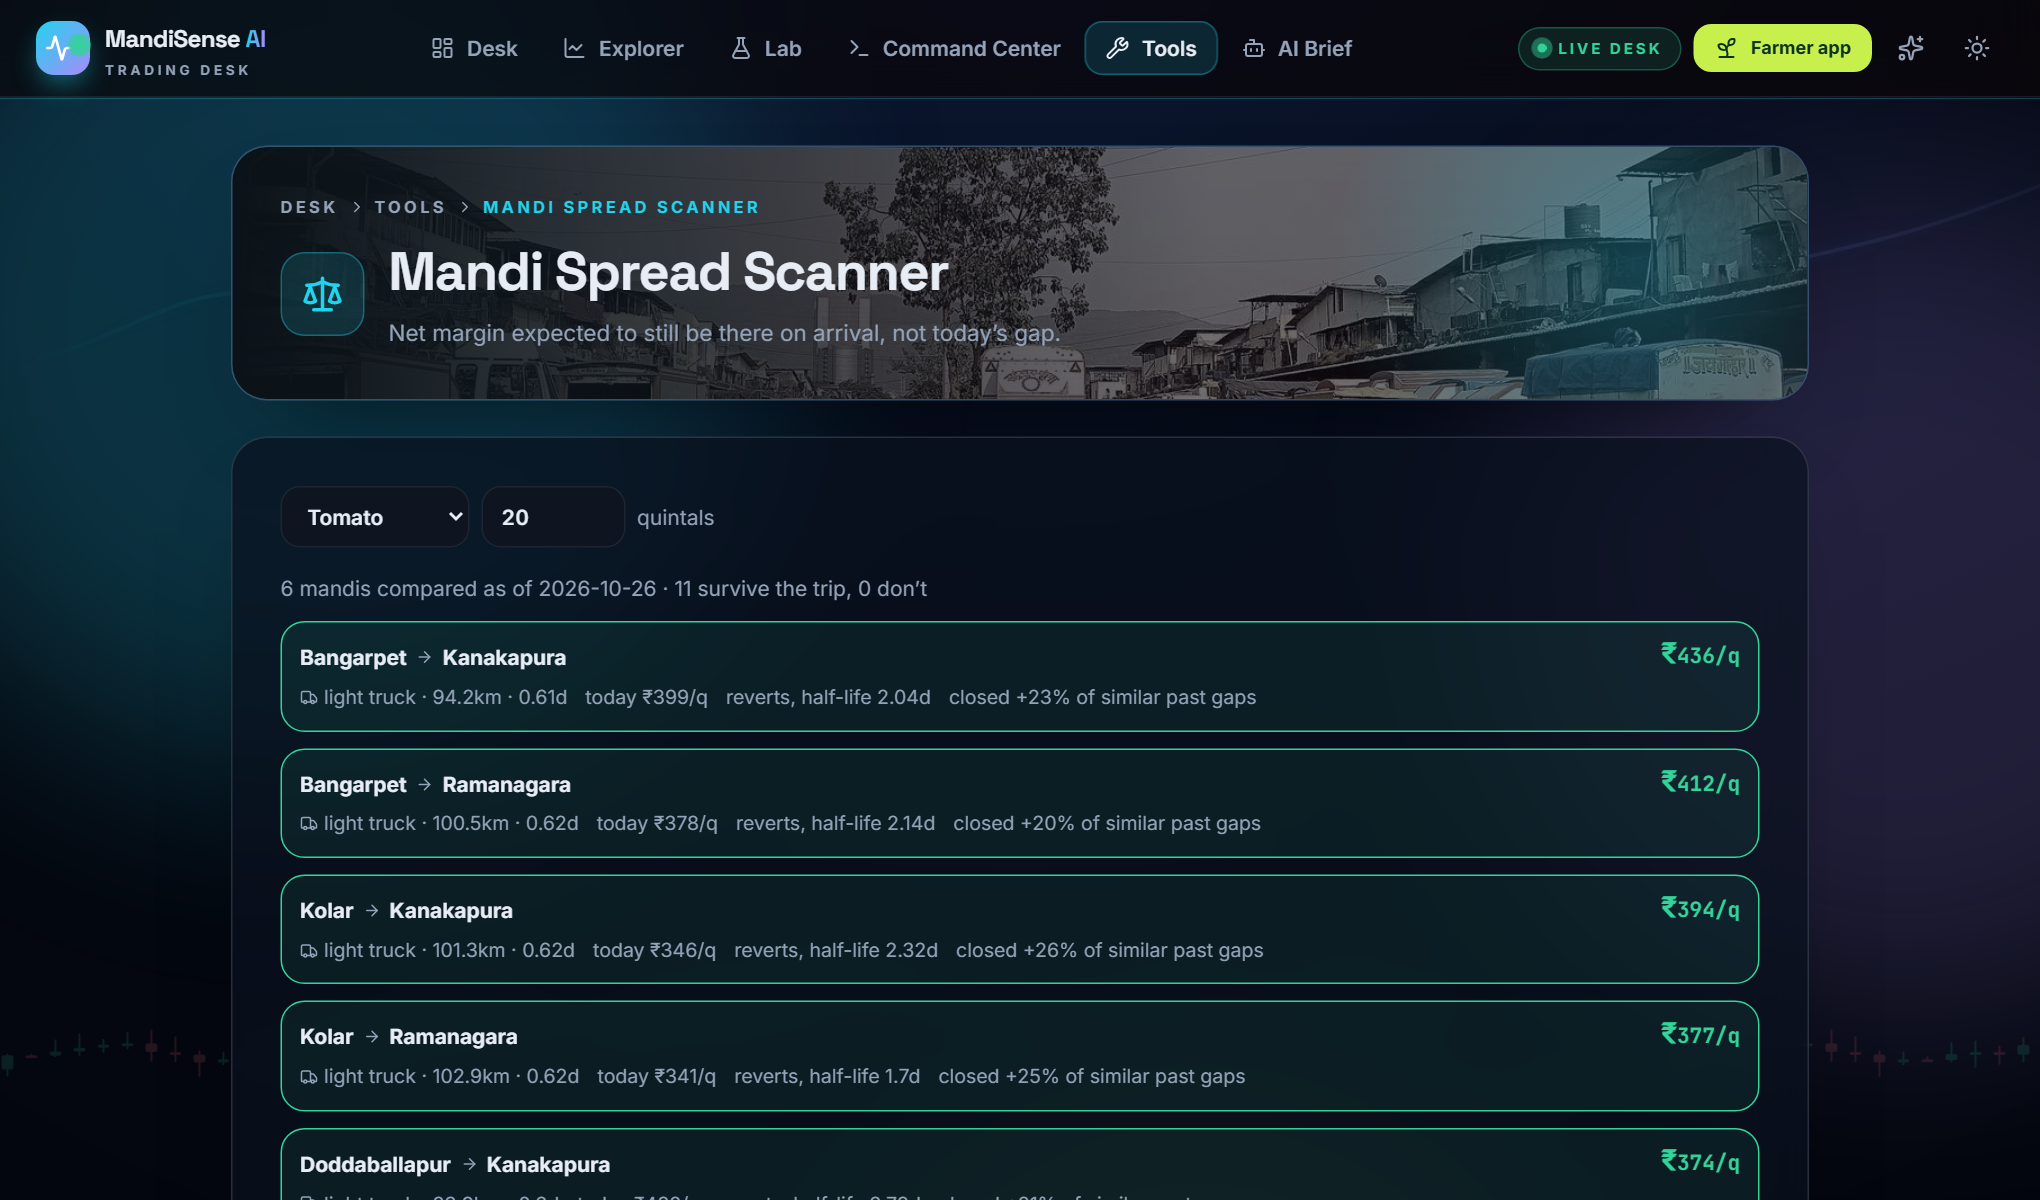
\includegraphics[width=0.93\linewidth]{figures/shot_w_spreads.png}}\\[0.5mm]{\footnotesize (a) Spreads between markets for one commodity}
\medskip
\fbox{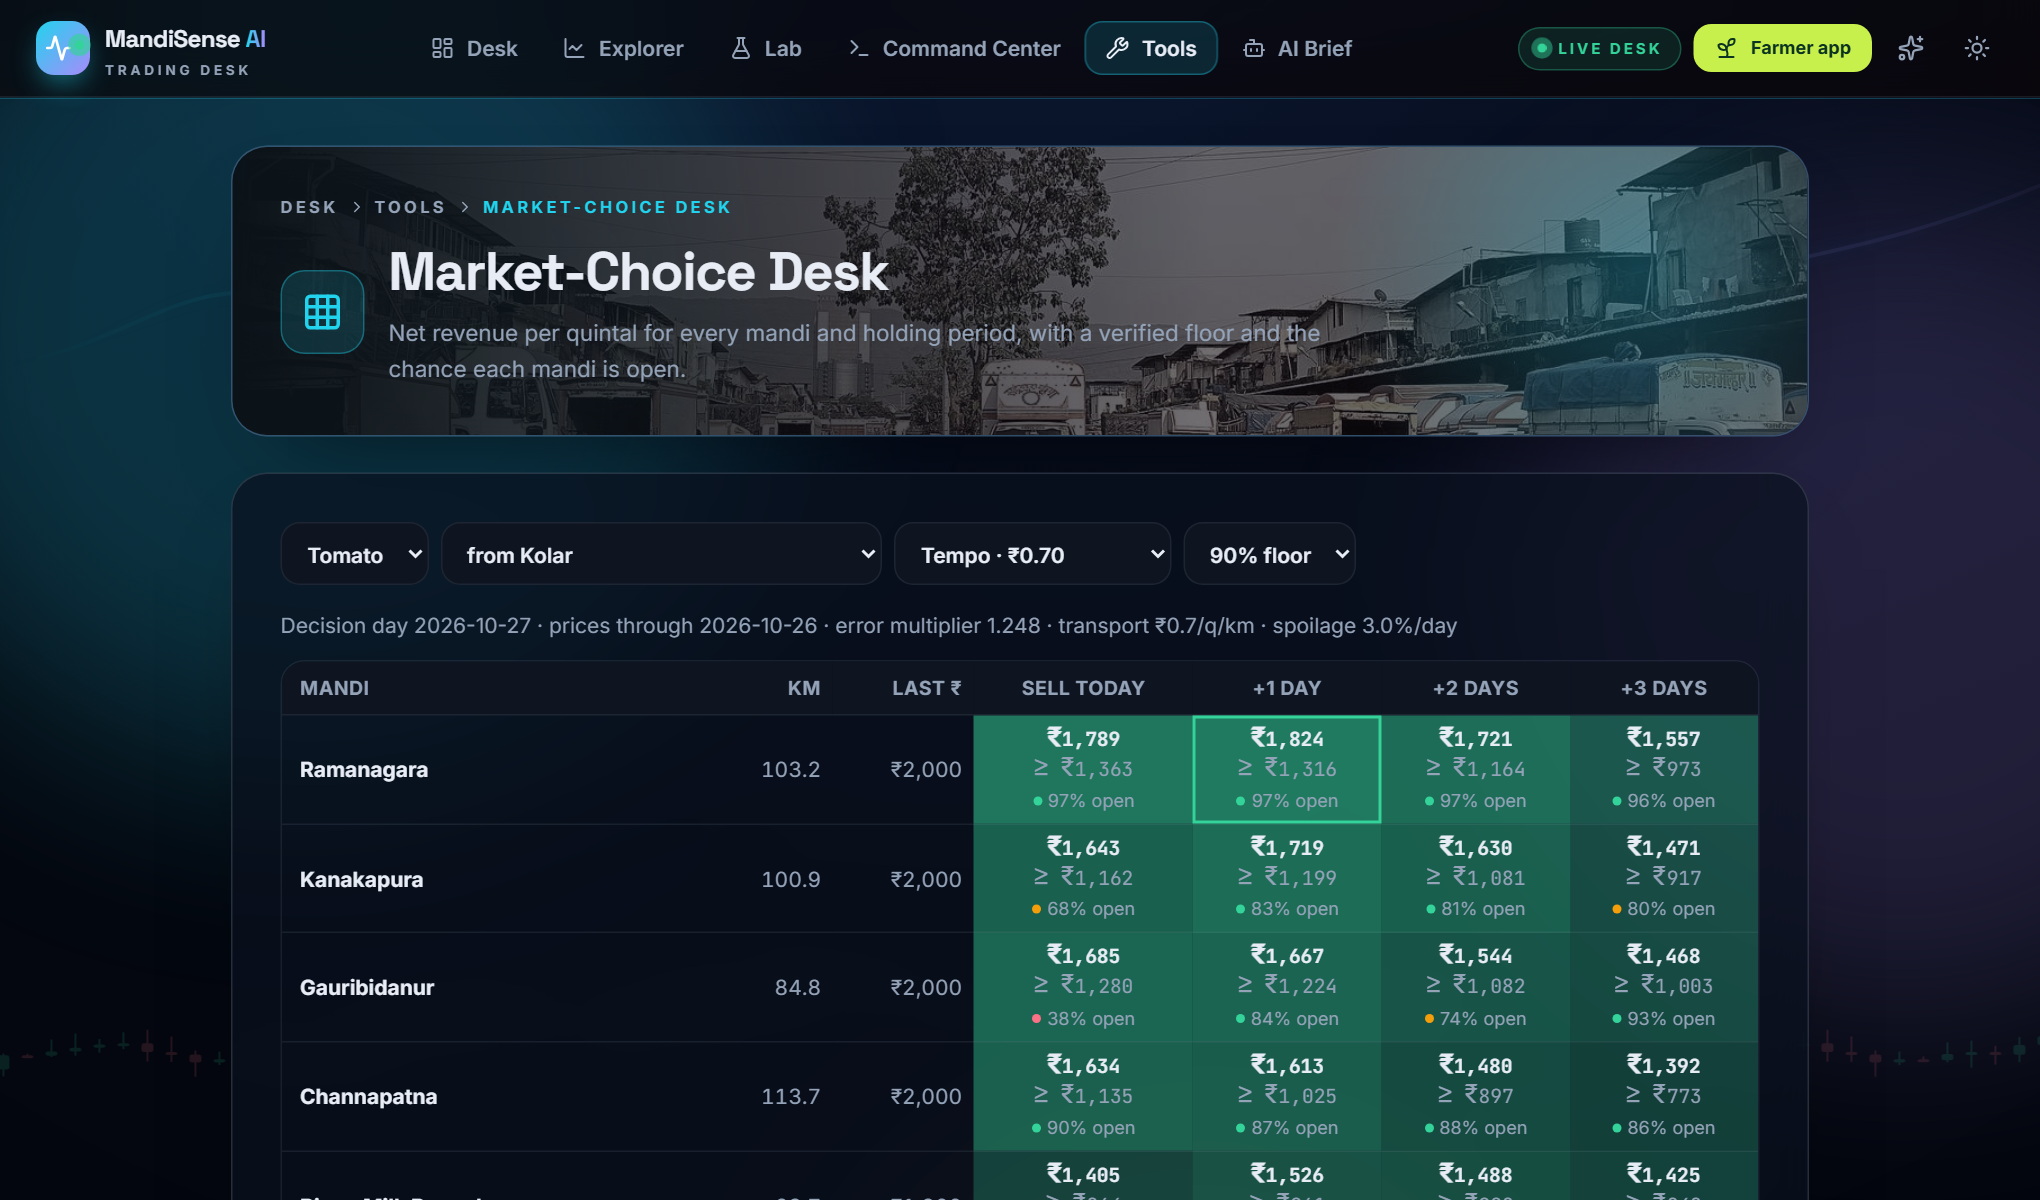
\includegraphics[width=0.93\linewidth]{figures/shot_w_mcdesk.png}}\\[0.5mm]{\footnotesize (b) The market-choice desk: the model's recommended market per day and the revenue floor}
\caption{(a) Spreads between markets for one commodity. (b) The market-choice desk: the model's recommended market per day and the revenue floor.}
\label{fig:sc-w-spreads}
\end{figure}

The spread tool shows the price gap between pairs of markets after transport, with the number of days each gap has lasted. A gap that persists is a signal of a market that is slow to clear.

This is the technical view of the recommendation of Section~\ref{sec:floors}: the chosen market, the expected and floor revenue, the alternatives and the model that produced them.

\begin{figure}[!t]
\centering
\fbox{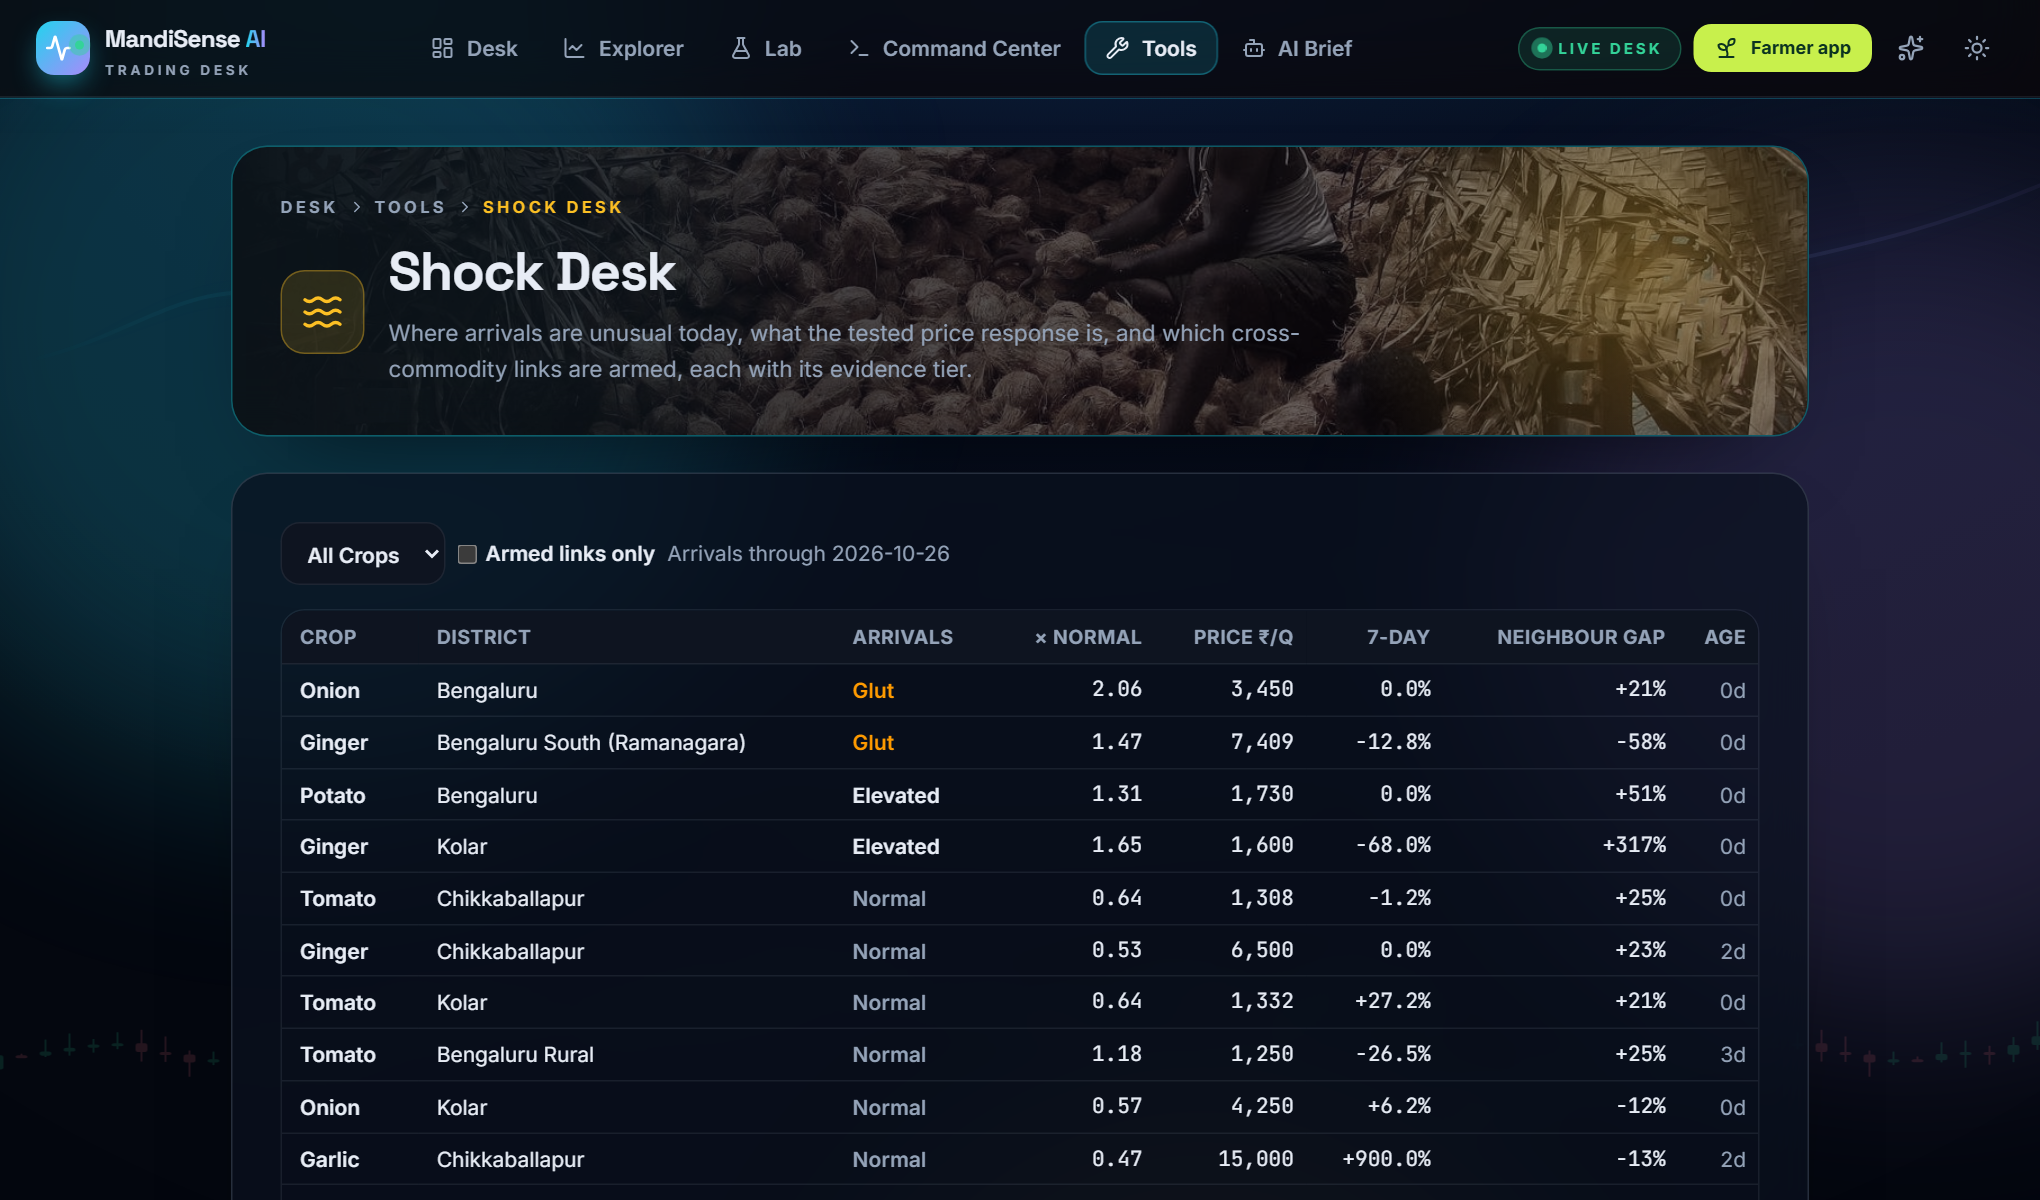
\includegraphics[width=0.93\linewidth]{figures/shot_w_shock.png}}\\[0.5mm]{\footnotesize (a) The shock desk: unusual price moves, with the markets affected}
\medskip
\fbox{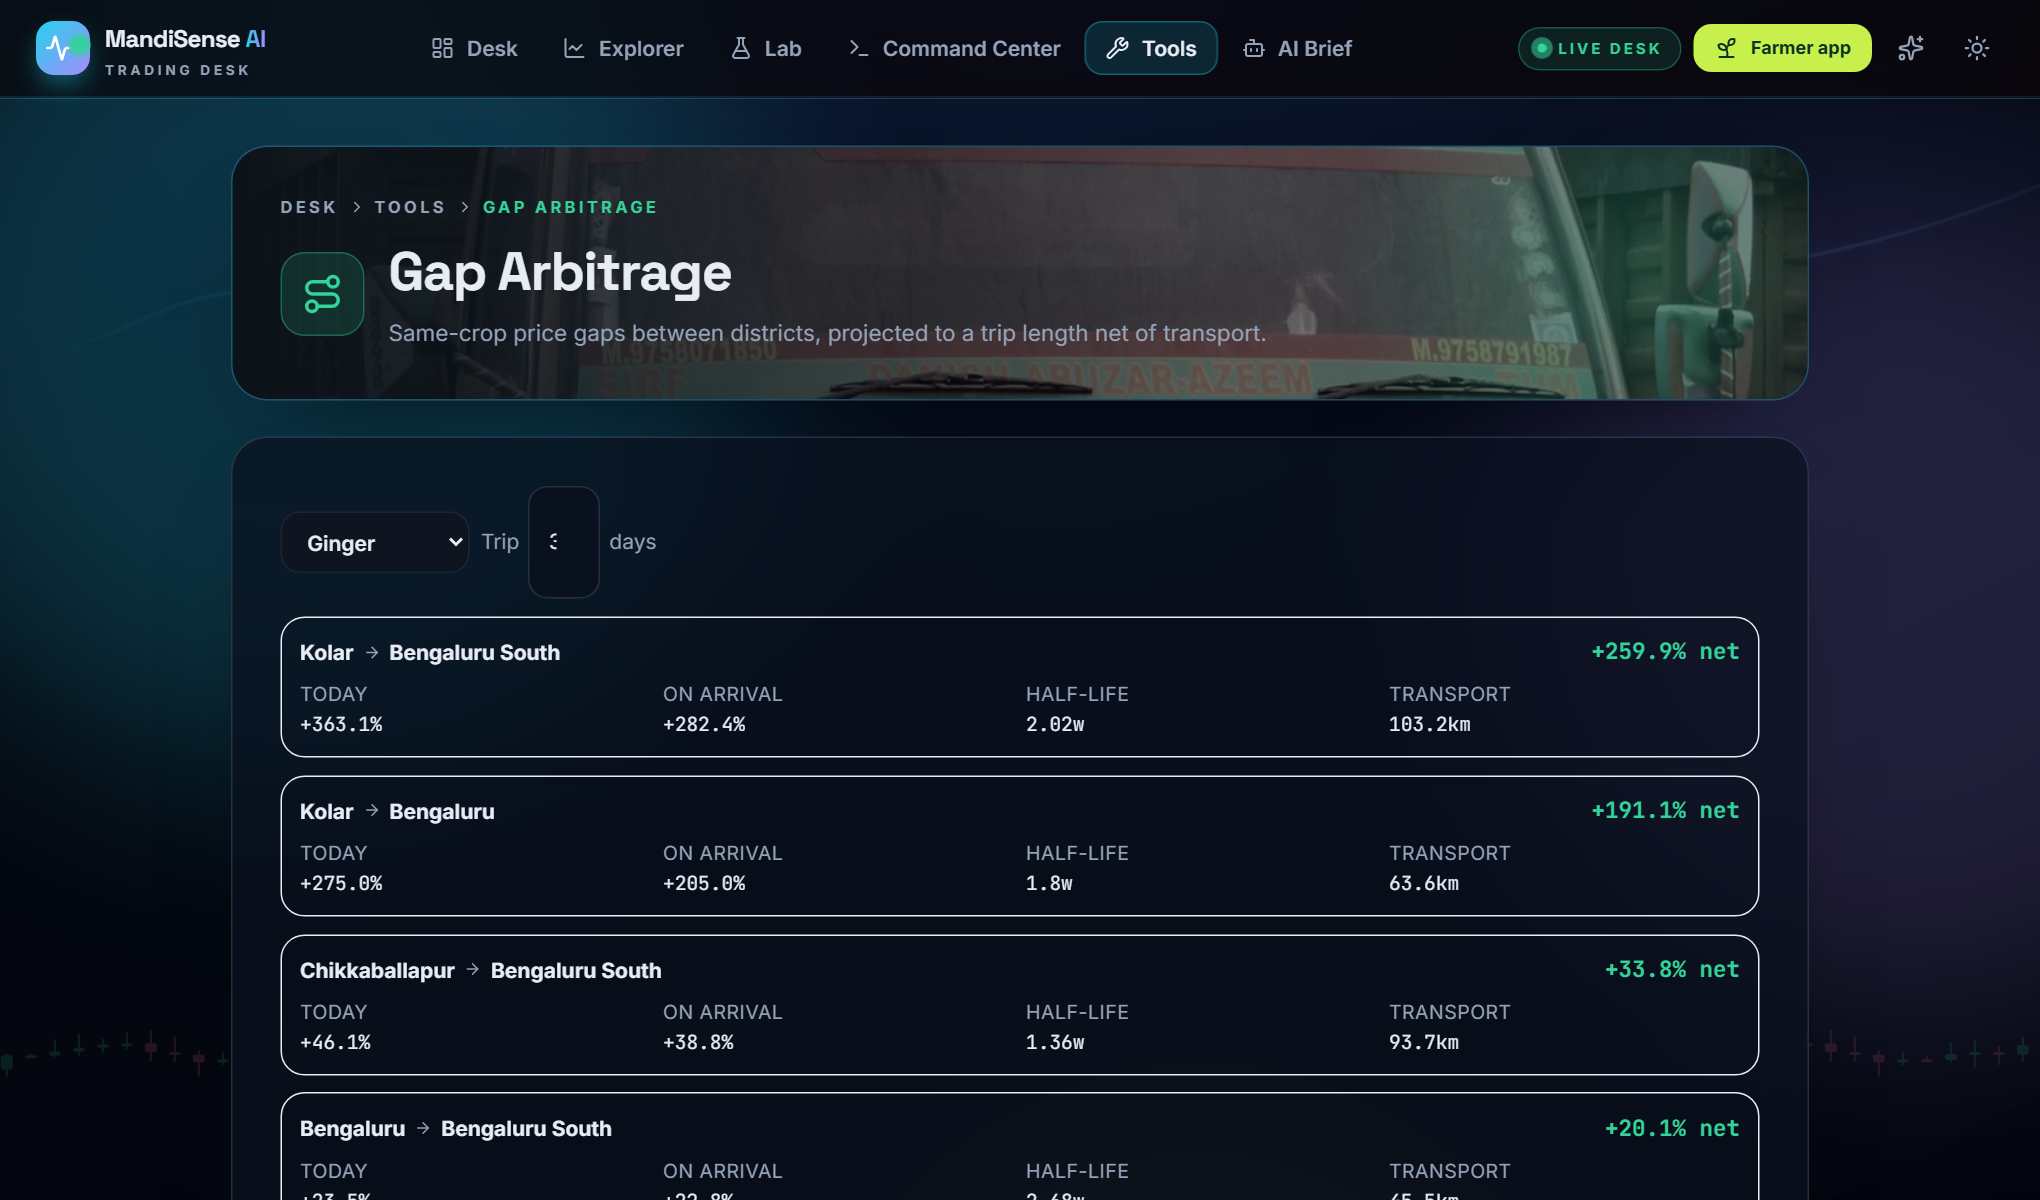
\includegraphics[width=0.93\linewidth]{figures/shot_w_gap.png}}\\[0.5mm]{\footnotesize (b) Gap arbitrage between mandis}
\caption{(a) The shock desk: unusual price moves, with the markets affected. (b) Gap arbitrage between mandis.}
\label{fig:sc-w-shock}
\end{figure}

The desk lists price moves that are unusual relative to a rolling baseline and the markets where they appear. It feeds the shock episodes used for the transmission test of Section~\ref{sec:spill-method}.

The tool pairs a high-price and a low-price market, deducts transport and shrinkage, and shows whether a gap is worth acting on.

\begin{figure}[!t]
\centering
\fbox{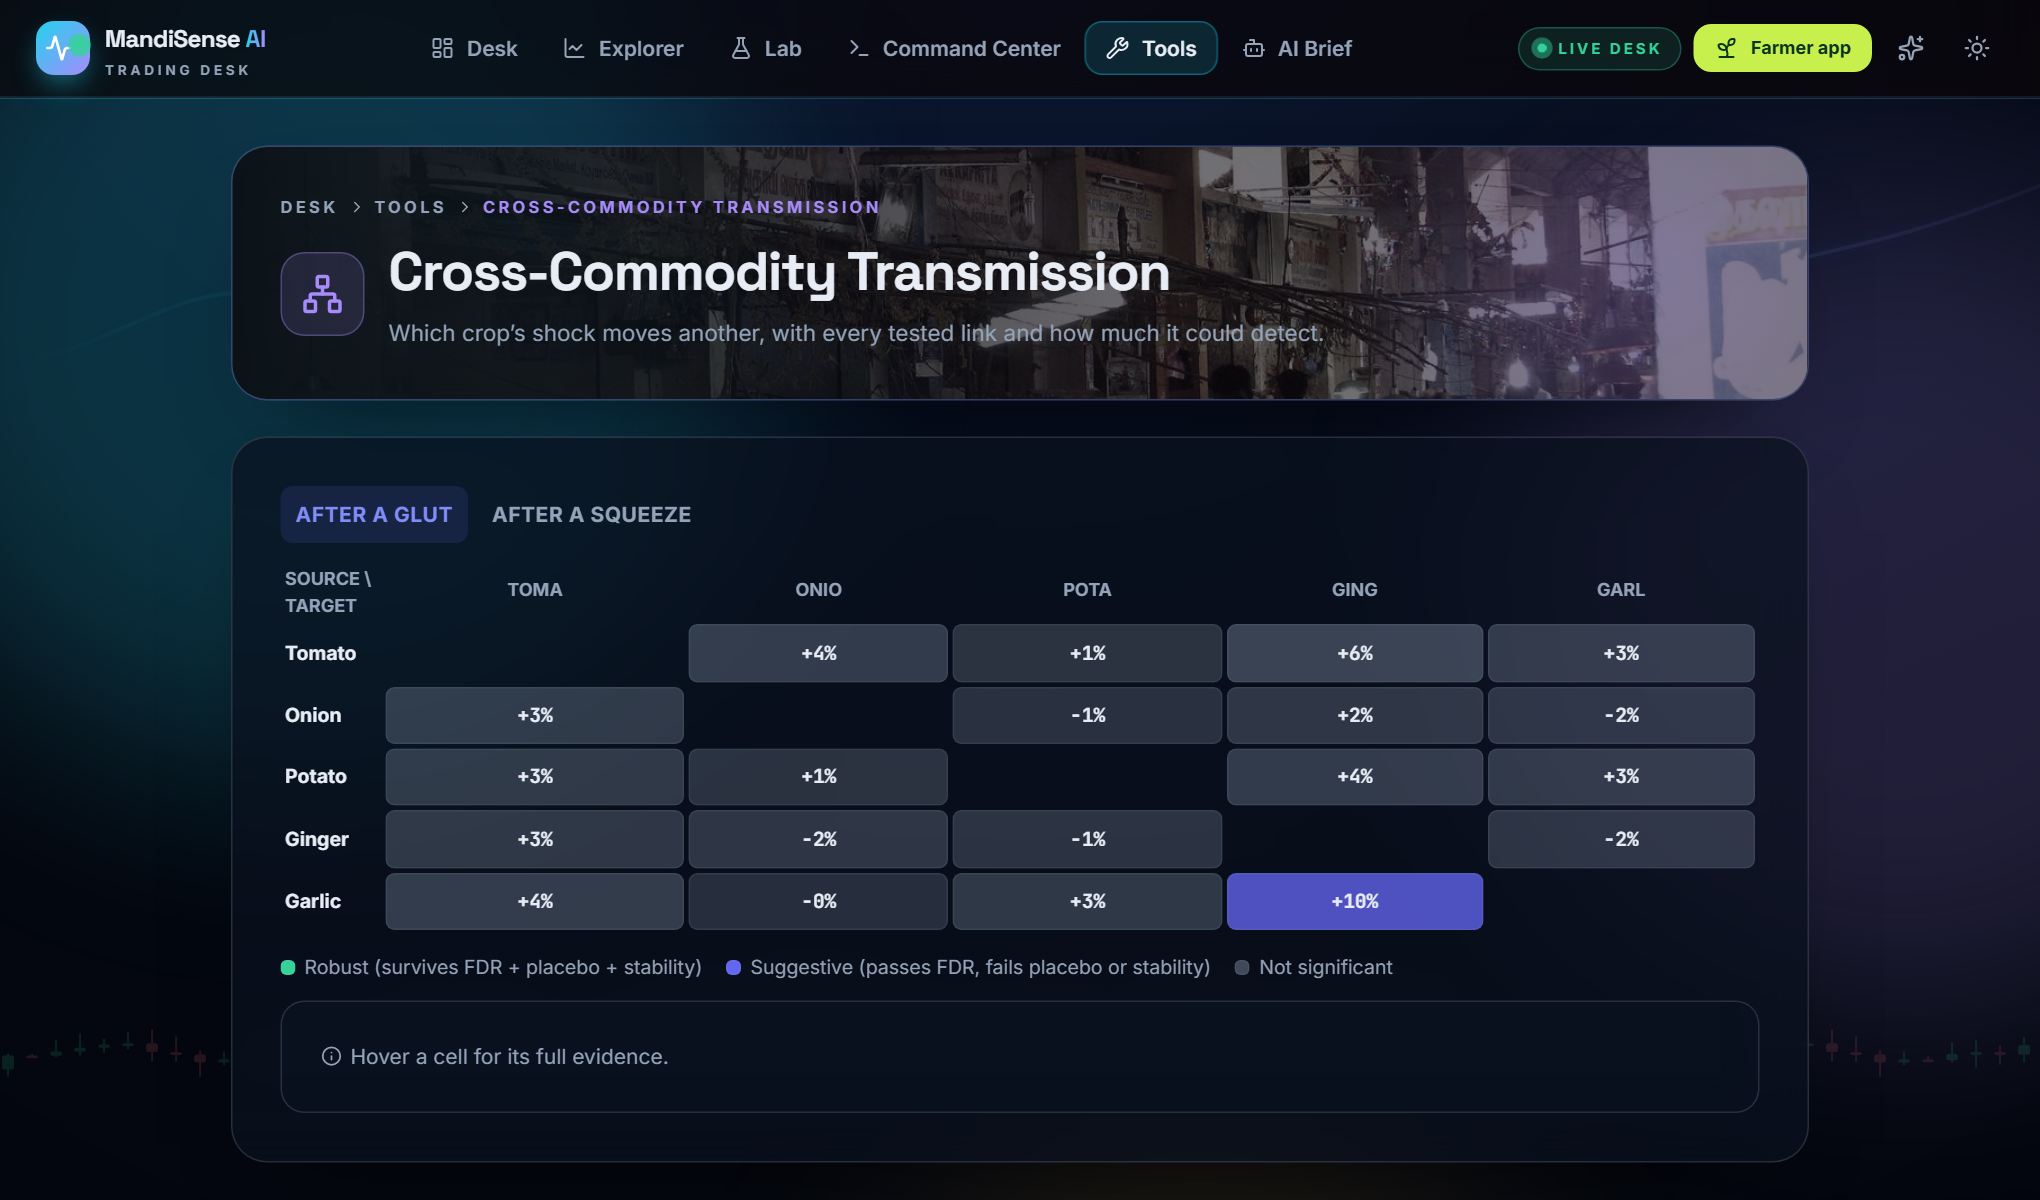
\includegraphics[width=0.93\linewidth]{figures/shot_w_transmission.png}}\\[0.5mm]{\footnotesize (a) Cross-commodity transmission}
\medskip
\fbox{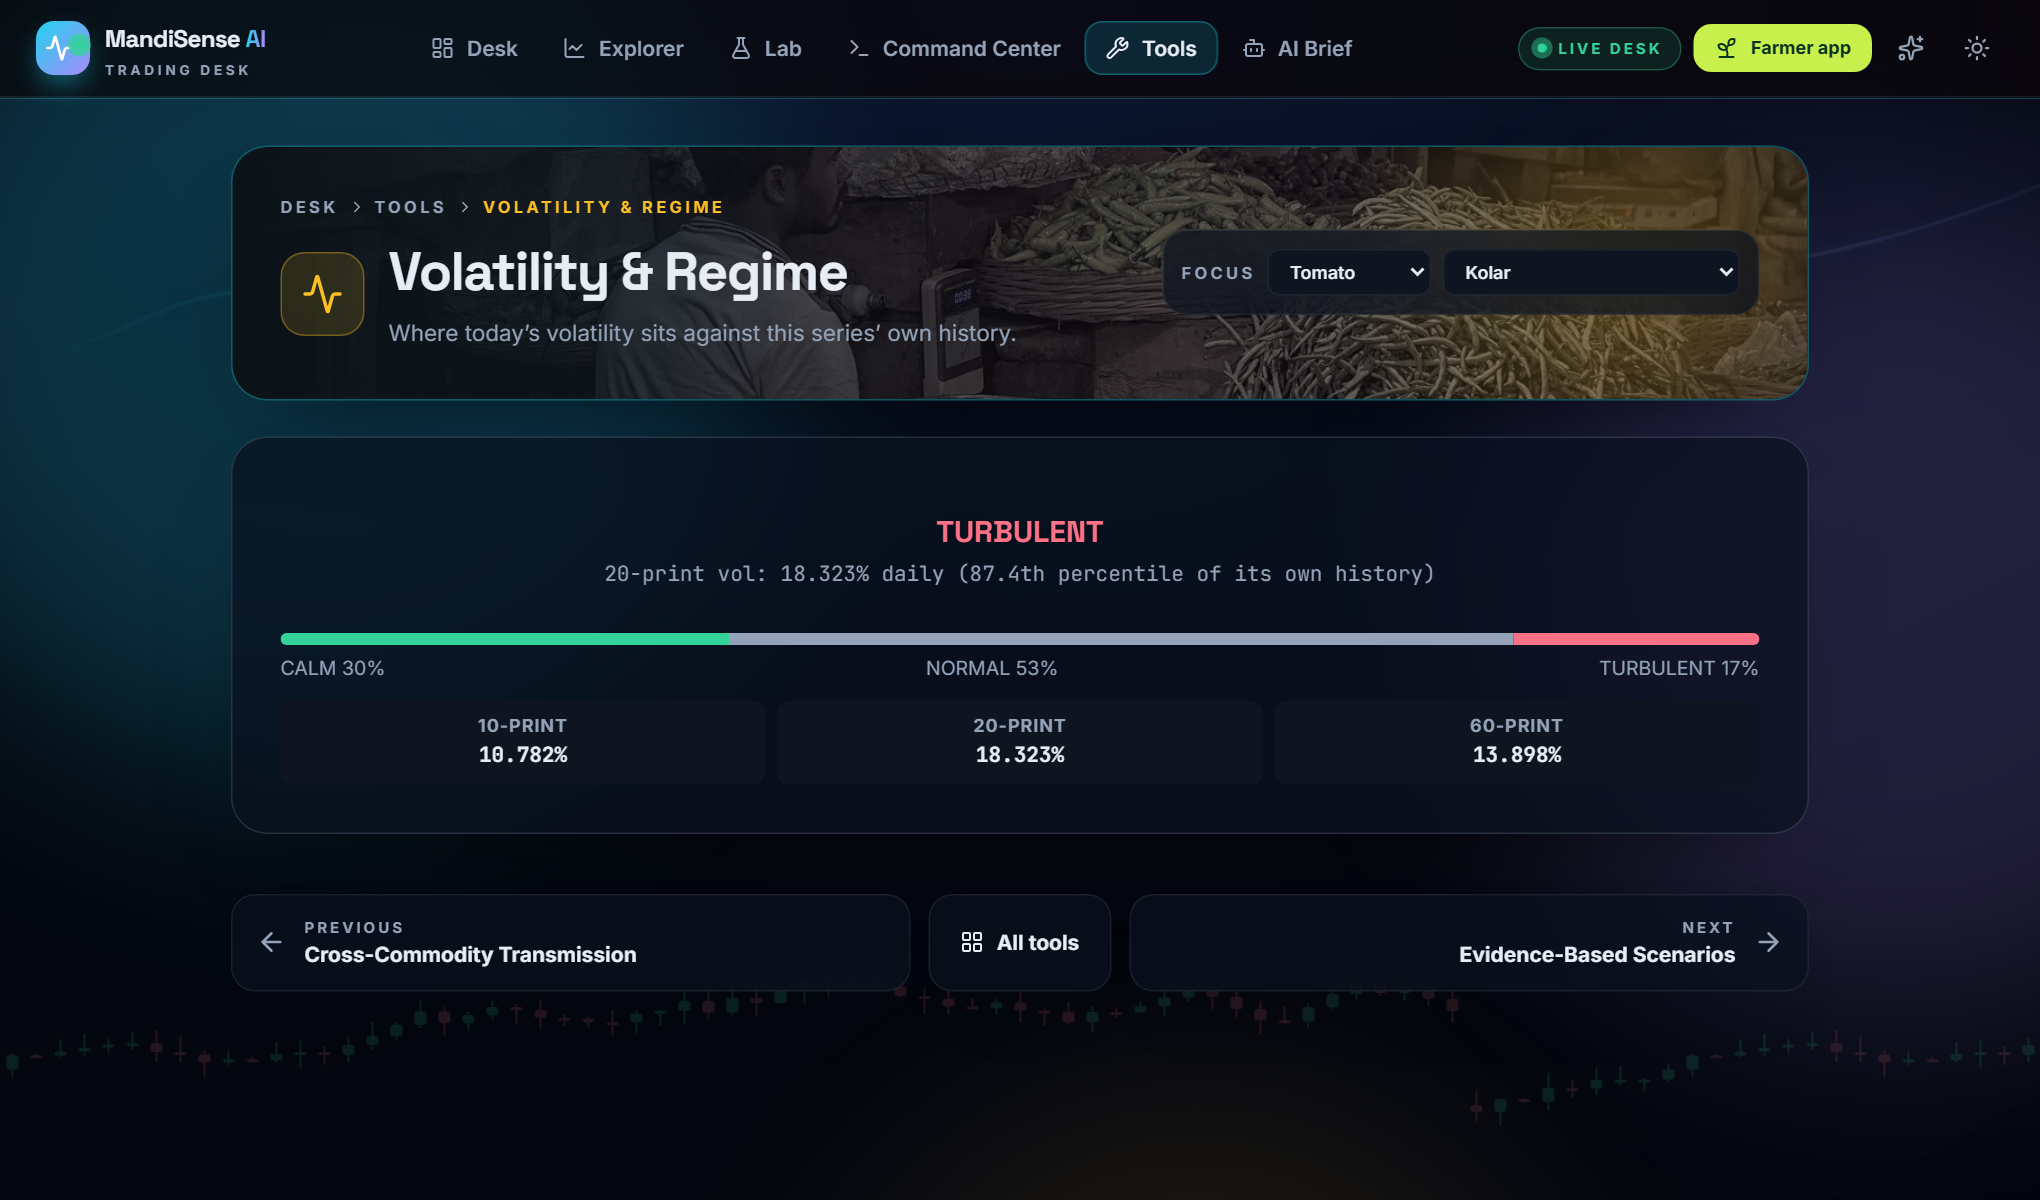
\includegraphics[width=0.93\linewidth]{figures/shot_w_volatility.png}}\\[0.5mm]{\footnotesize (b) Price volatility by commodity and market}
\caption{(a) Cross-commodity transmission. (b) Price volatility by commodity and market.}
\label{fig:sc-w-transmission}
\end{figure}

The transmission page shows the estimated response of one crop to a shock in another. When the evidence is too thin the page says so and shows no number, which is the withholding behaviour described in Section~\ref{sec:transmission}.

Rolling volatility of each series, which the farmer pages translate into a plain warning when a price is unusually unsettled.

\begin{figure}[!t]
\centering
\fbox{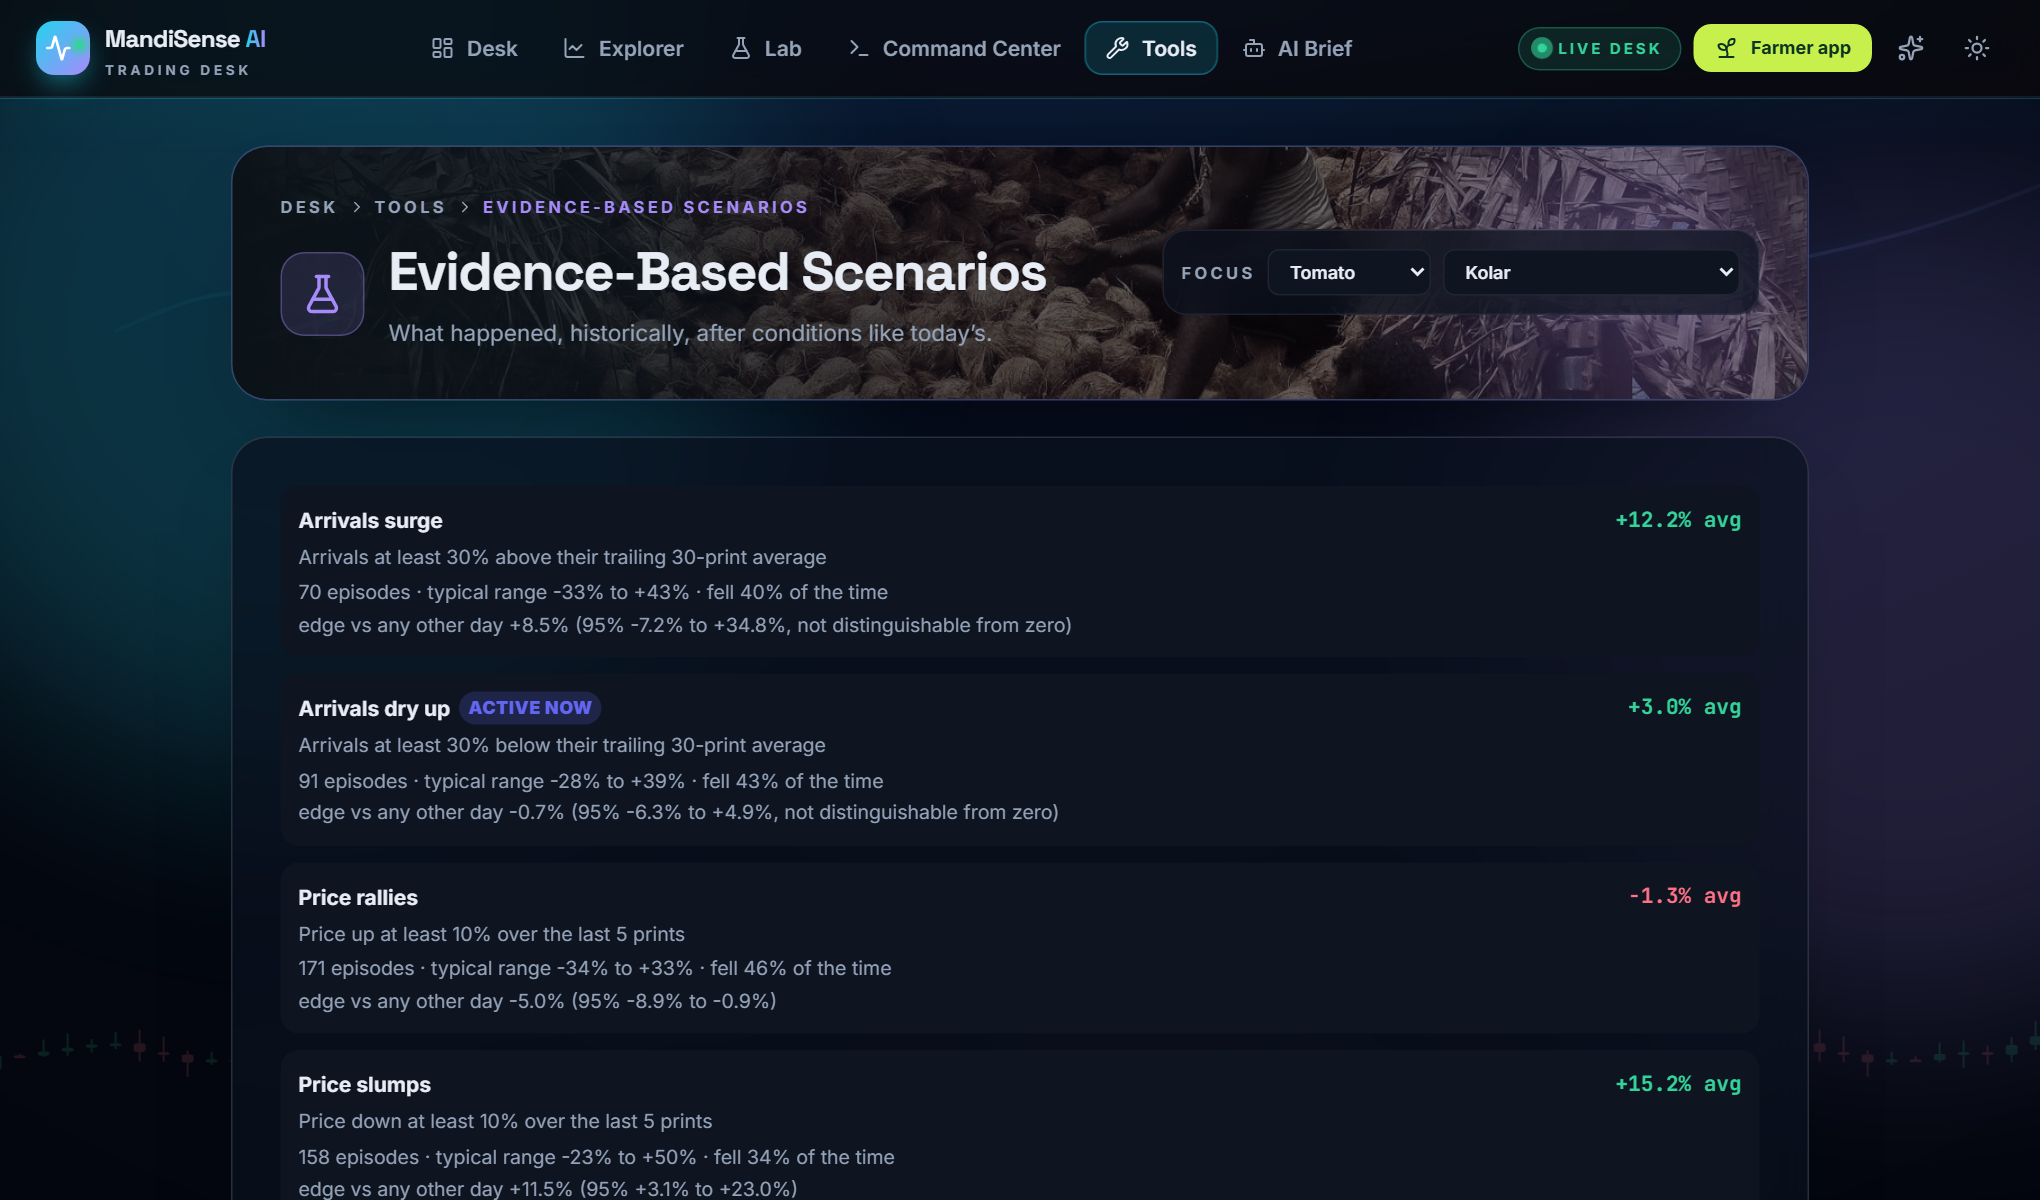
\includegraphics[width=0.93\linewidth]{figures/shot_w_scenarios.png}}\\[0.5mm]{\footnotesize (a) Scenario analysis for the revenue of a sale plan}
\medskip
\fbox{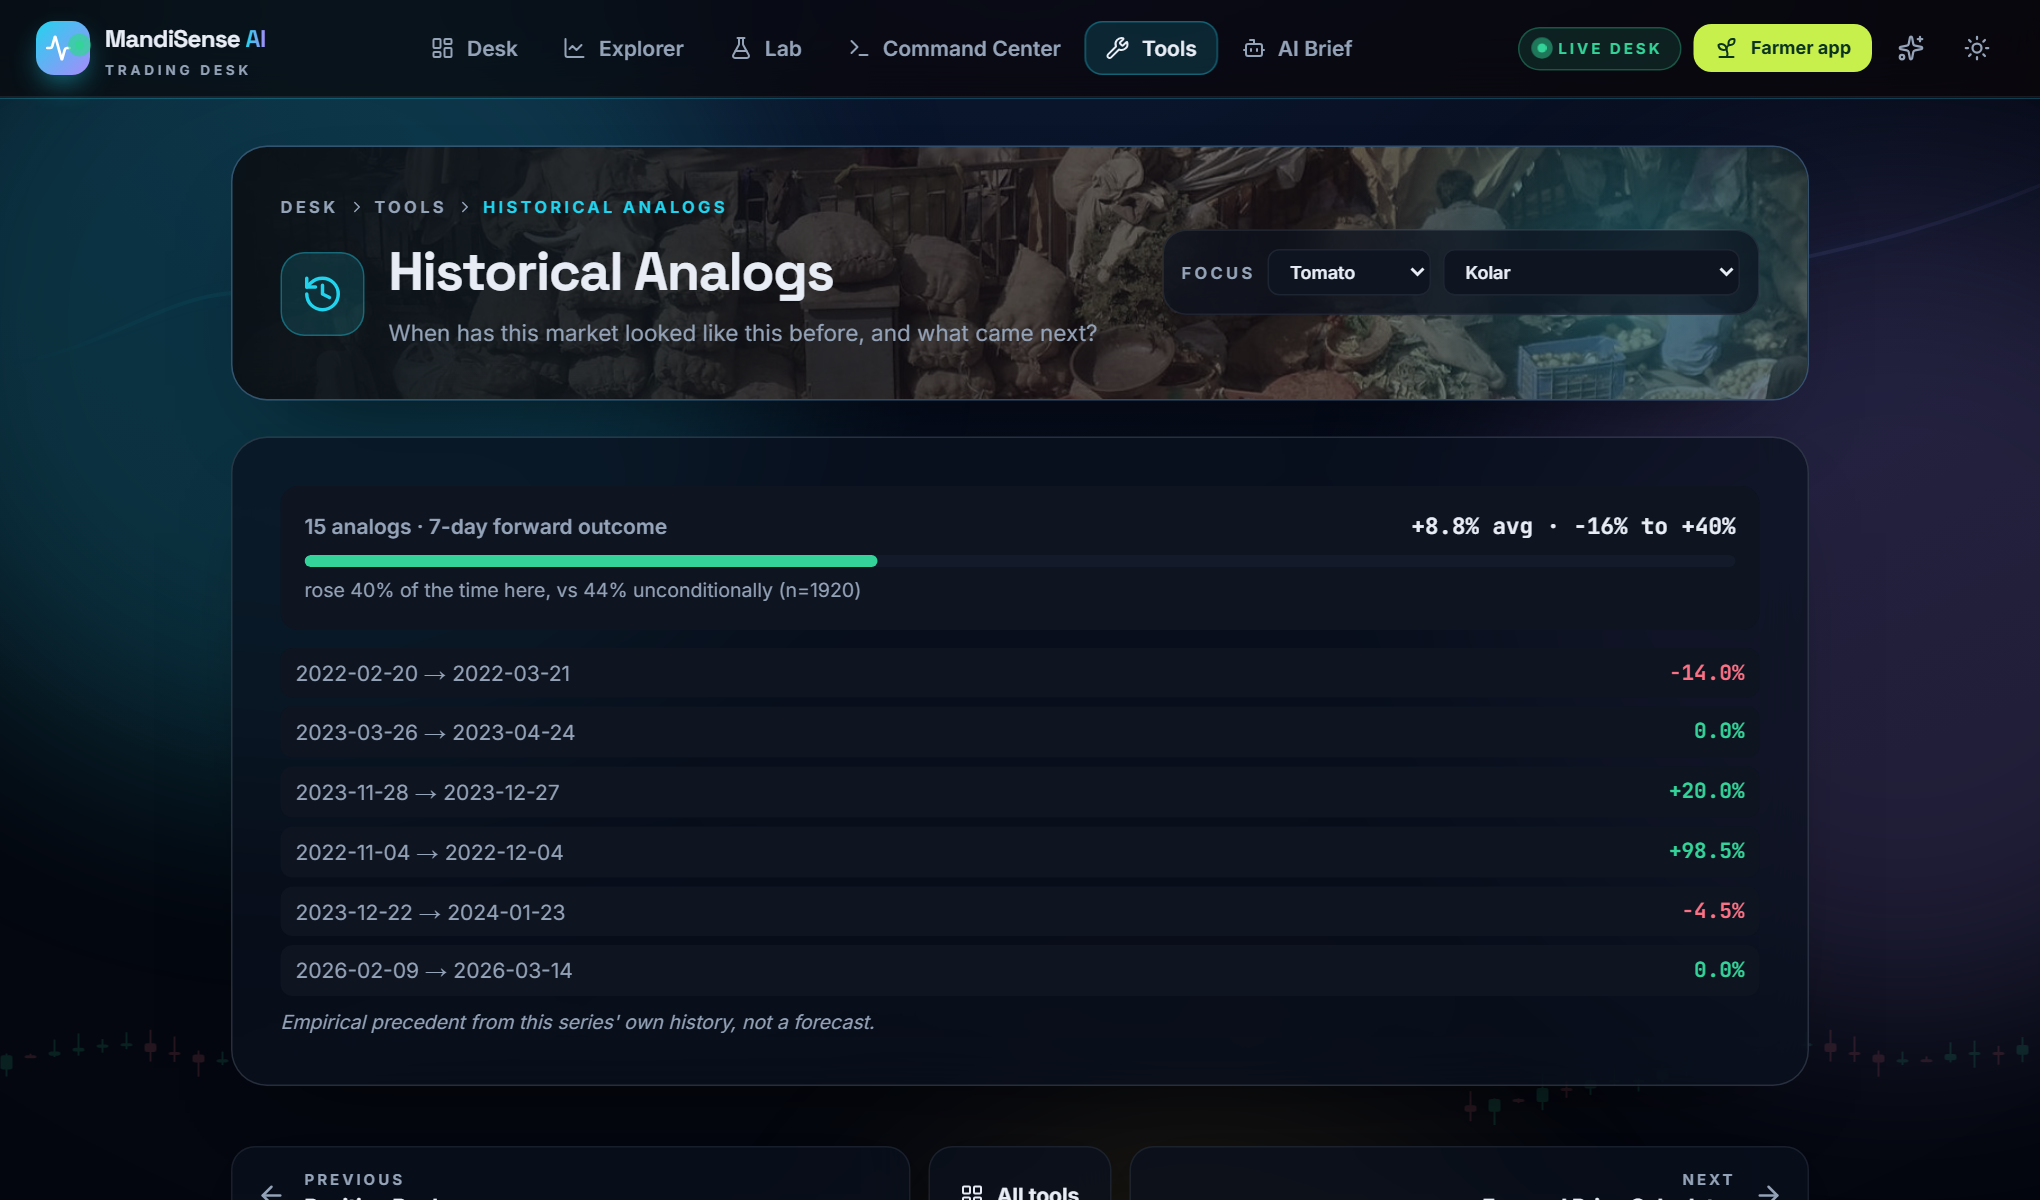
\includegraphics[width=0.93\linewidth]{figures/shot_w_analogs.png}}\\[0.5mm]{\footnotesize (b) Analog days: past days that resembled today}
\caption{(a) Scenario analysis for the revenue of a sale plan. (b) Analog days: past days that resembled today.}
\label{fig:sc-w-scenarios}
\end{figure}

The tool changes transport cost, shrinkage and price in turn and shows how the recommended choice and its revenue respond.

The page finds earlier days with a similar price pattern and shows what followed, as an aid to judgement and not as a forecast.

\begin{figure}[!t]
\centering
\fbox{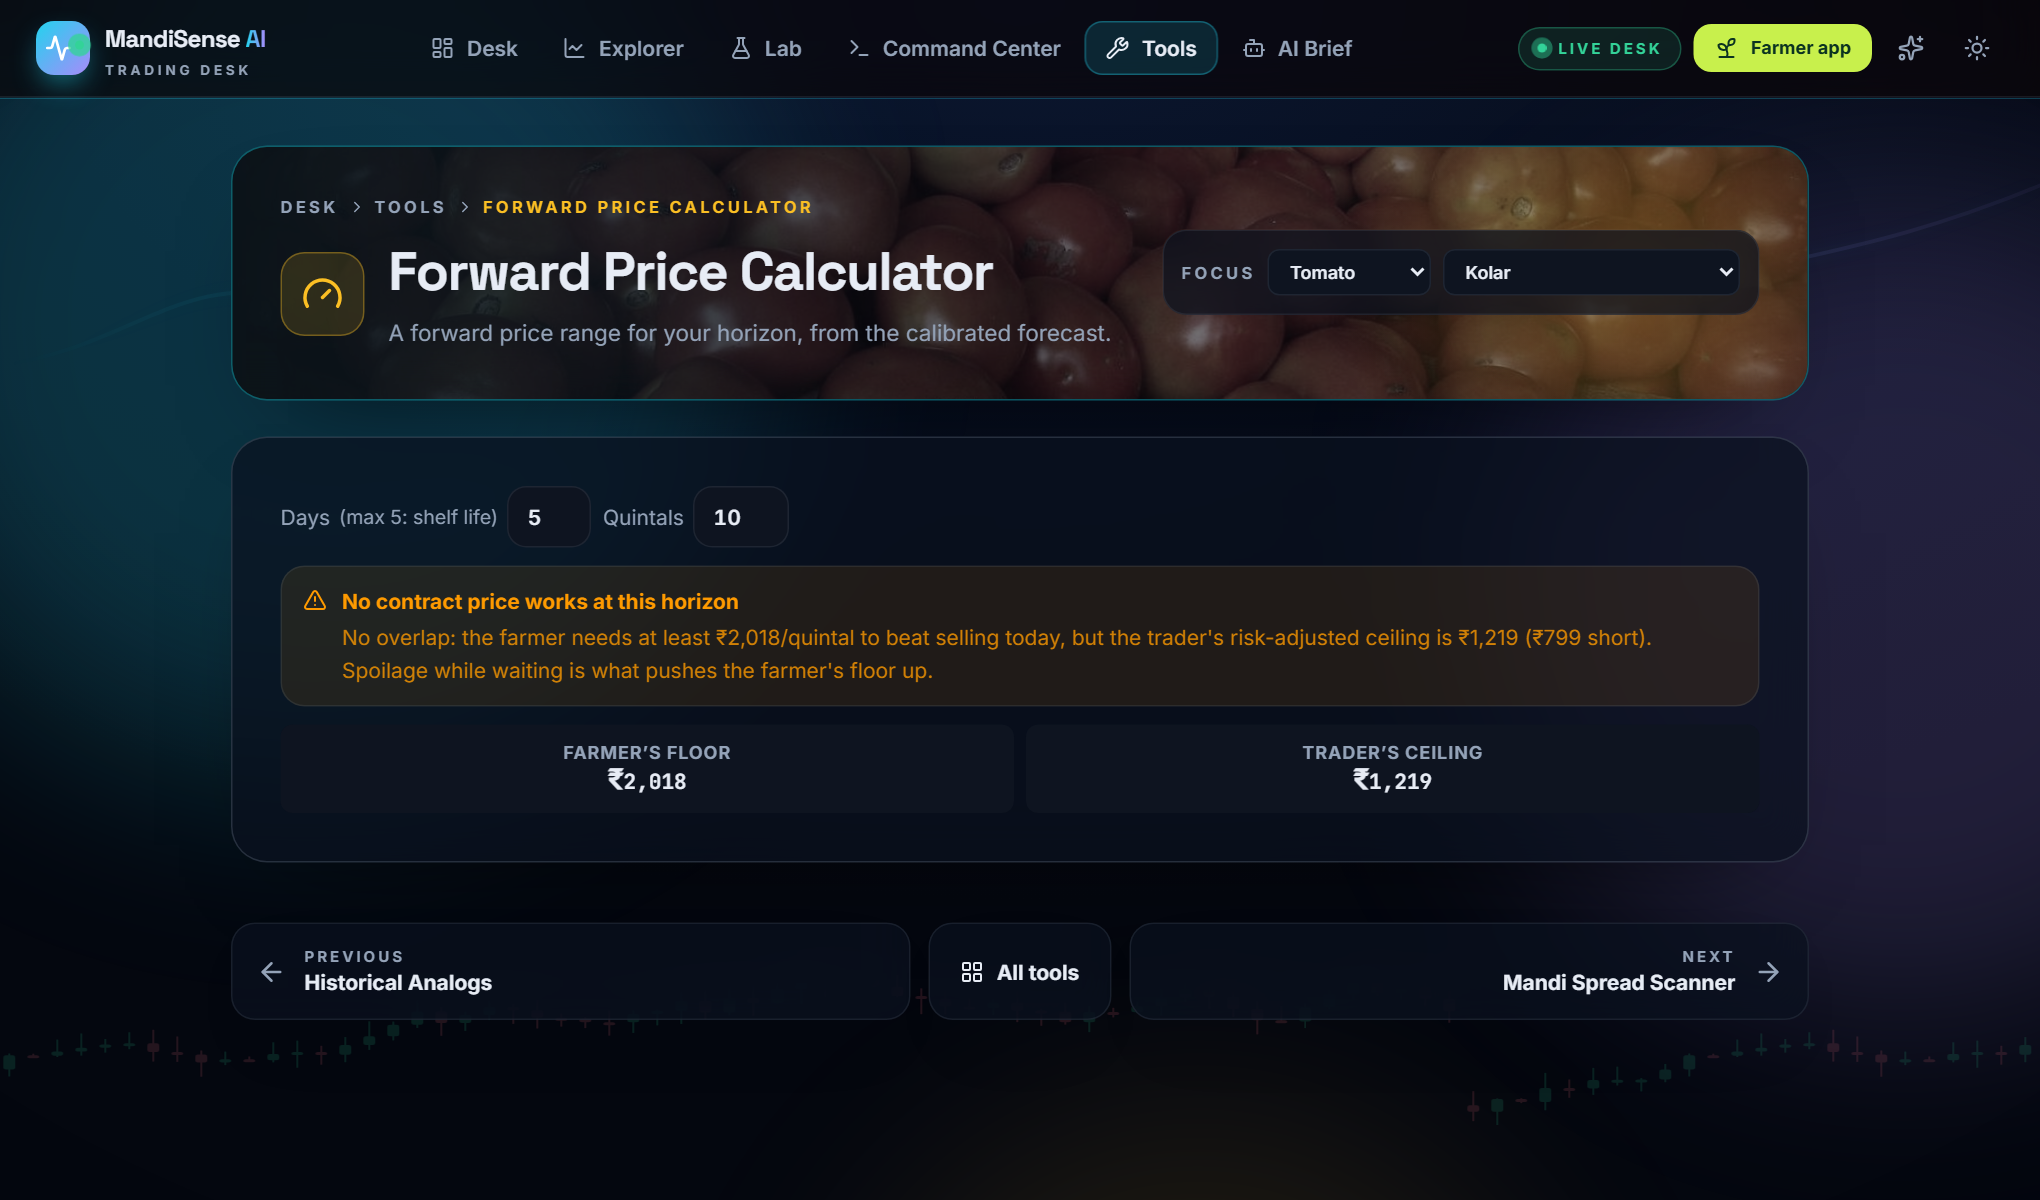
\includegraphics[width=0.93\linewidth]{figures/shot_w_forward.png}}\\[0.5mm]{\footnotesize (a) Forward price view}
\medskip
\fbox{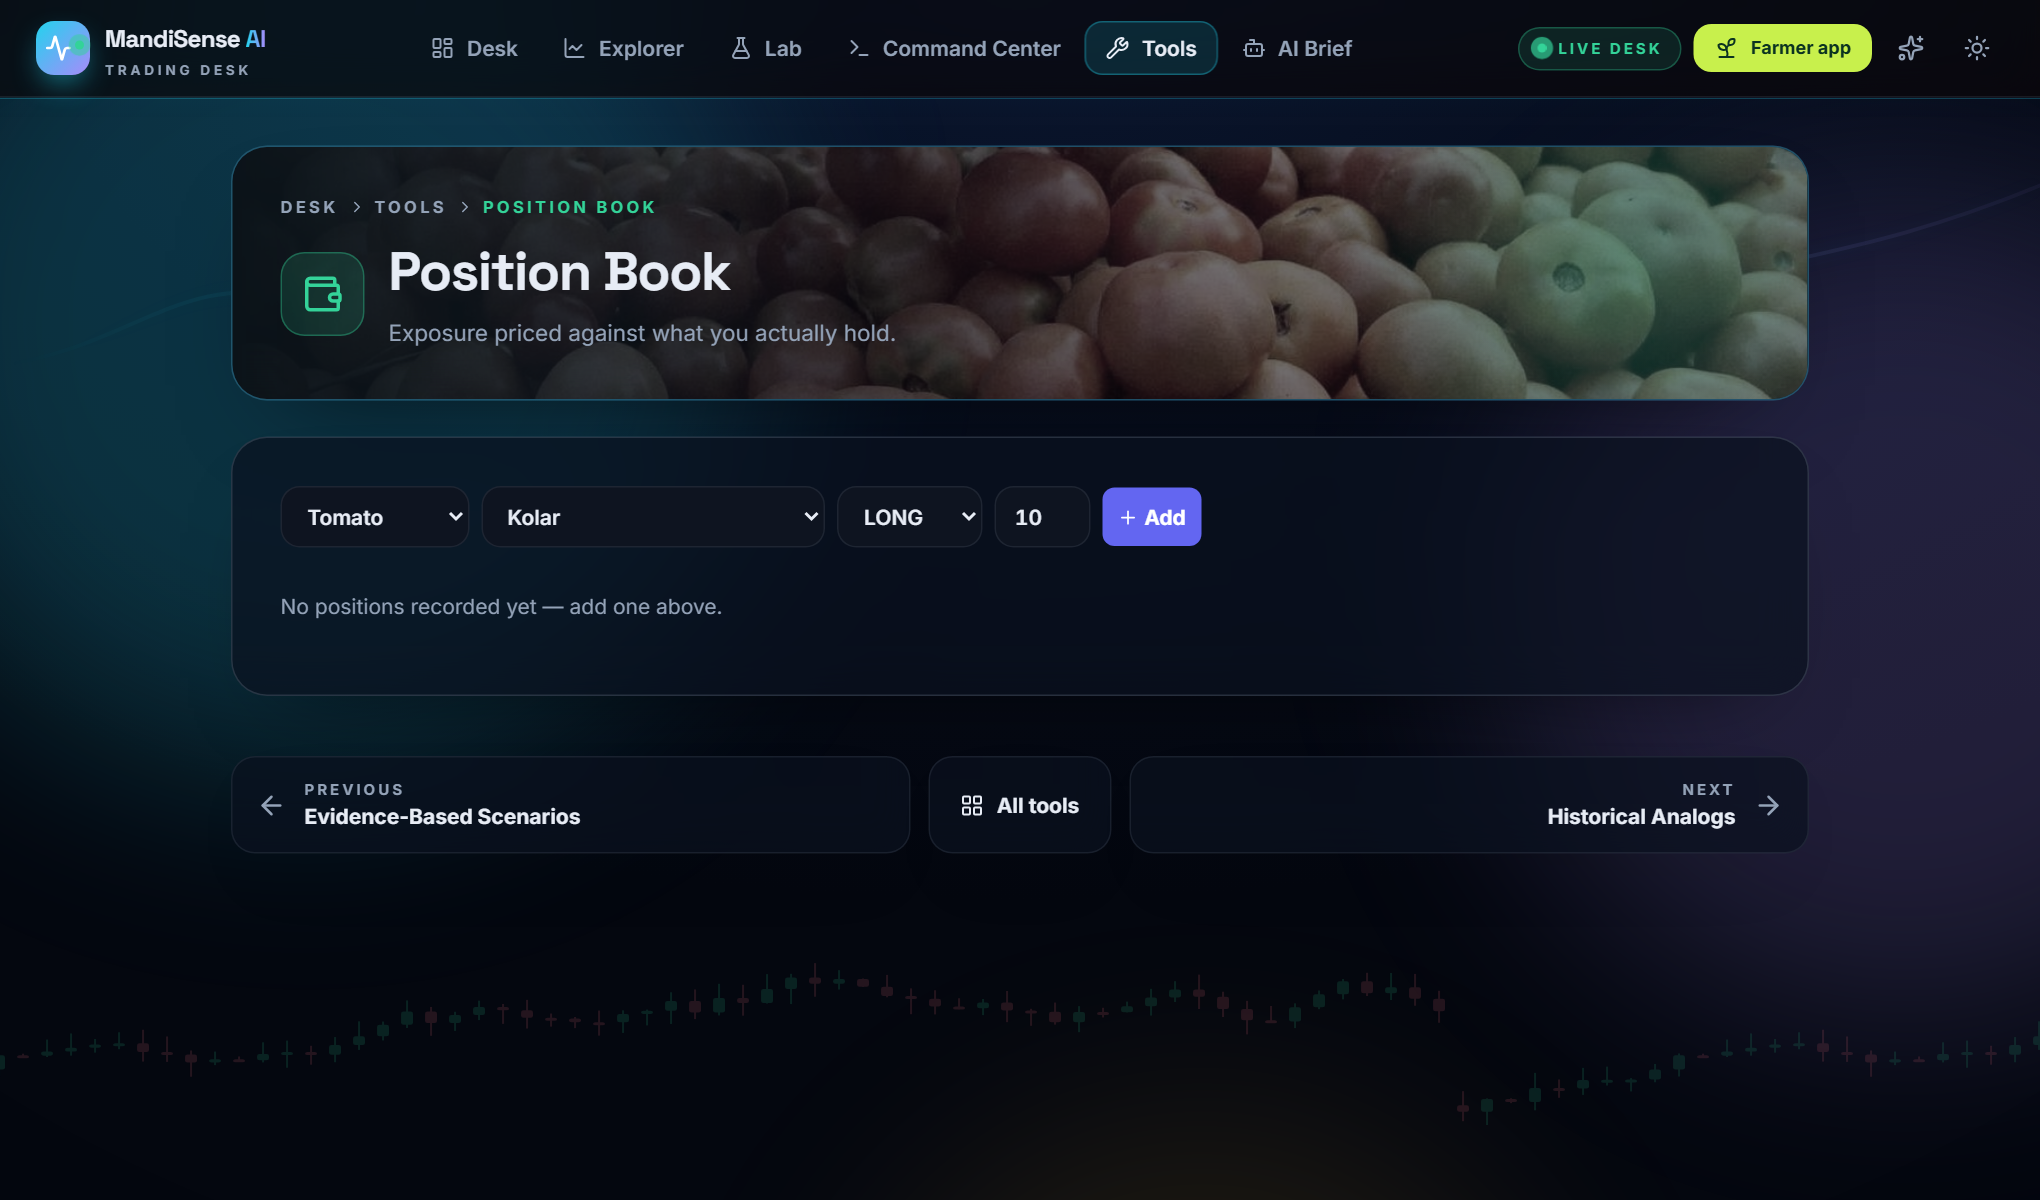
\includegraphics[width=0.93\linewidth]{figures/shot_w_positions.png}}\\[0.5mm]{\footnotesize (b) Positions: the sales a trader is tracking}
\caption{(a) Forward price view. (b) Positions: the sales a trader is tracking.}
\label{fig:sc-w-forward}
\end{figure}

A forecast with its interval for the coming days, with the forecasting model named on the page.

A small ledger of intended sales with their marked-to-market value.

\begin{figure}[!t]
\centering
\fbox{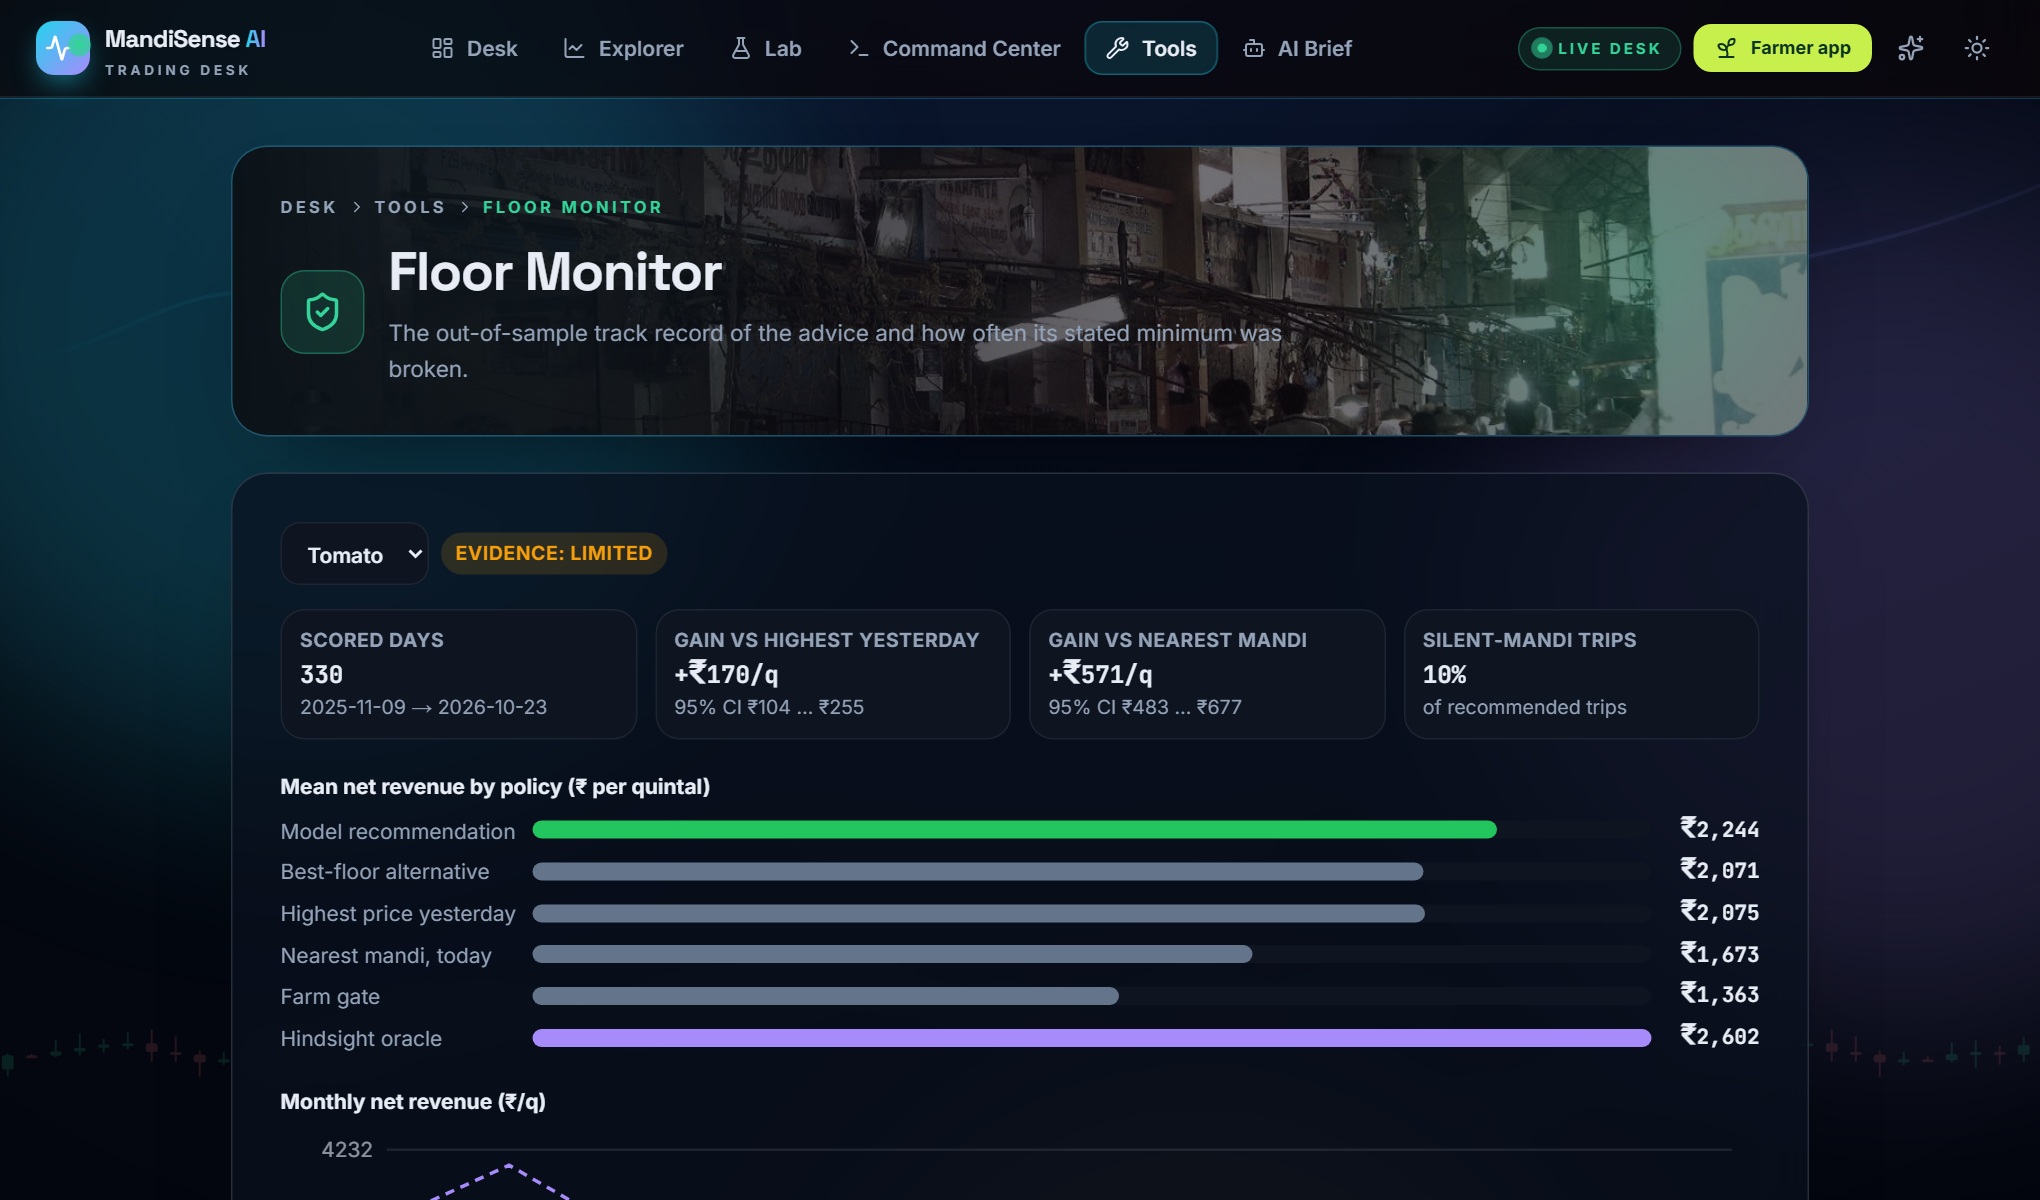
\includegraphics[width=0.93\linewidth]{figures/shot_w_floormon.png}}\\[0.5mm]{\footnotesize (a) Floor monitor: how often the revenue floor has held}
\medskip
\fbox{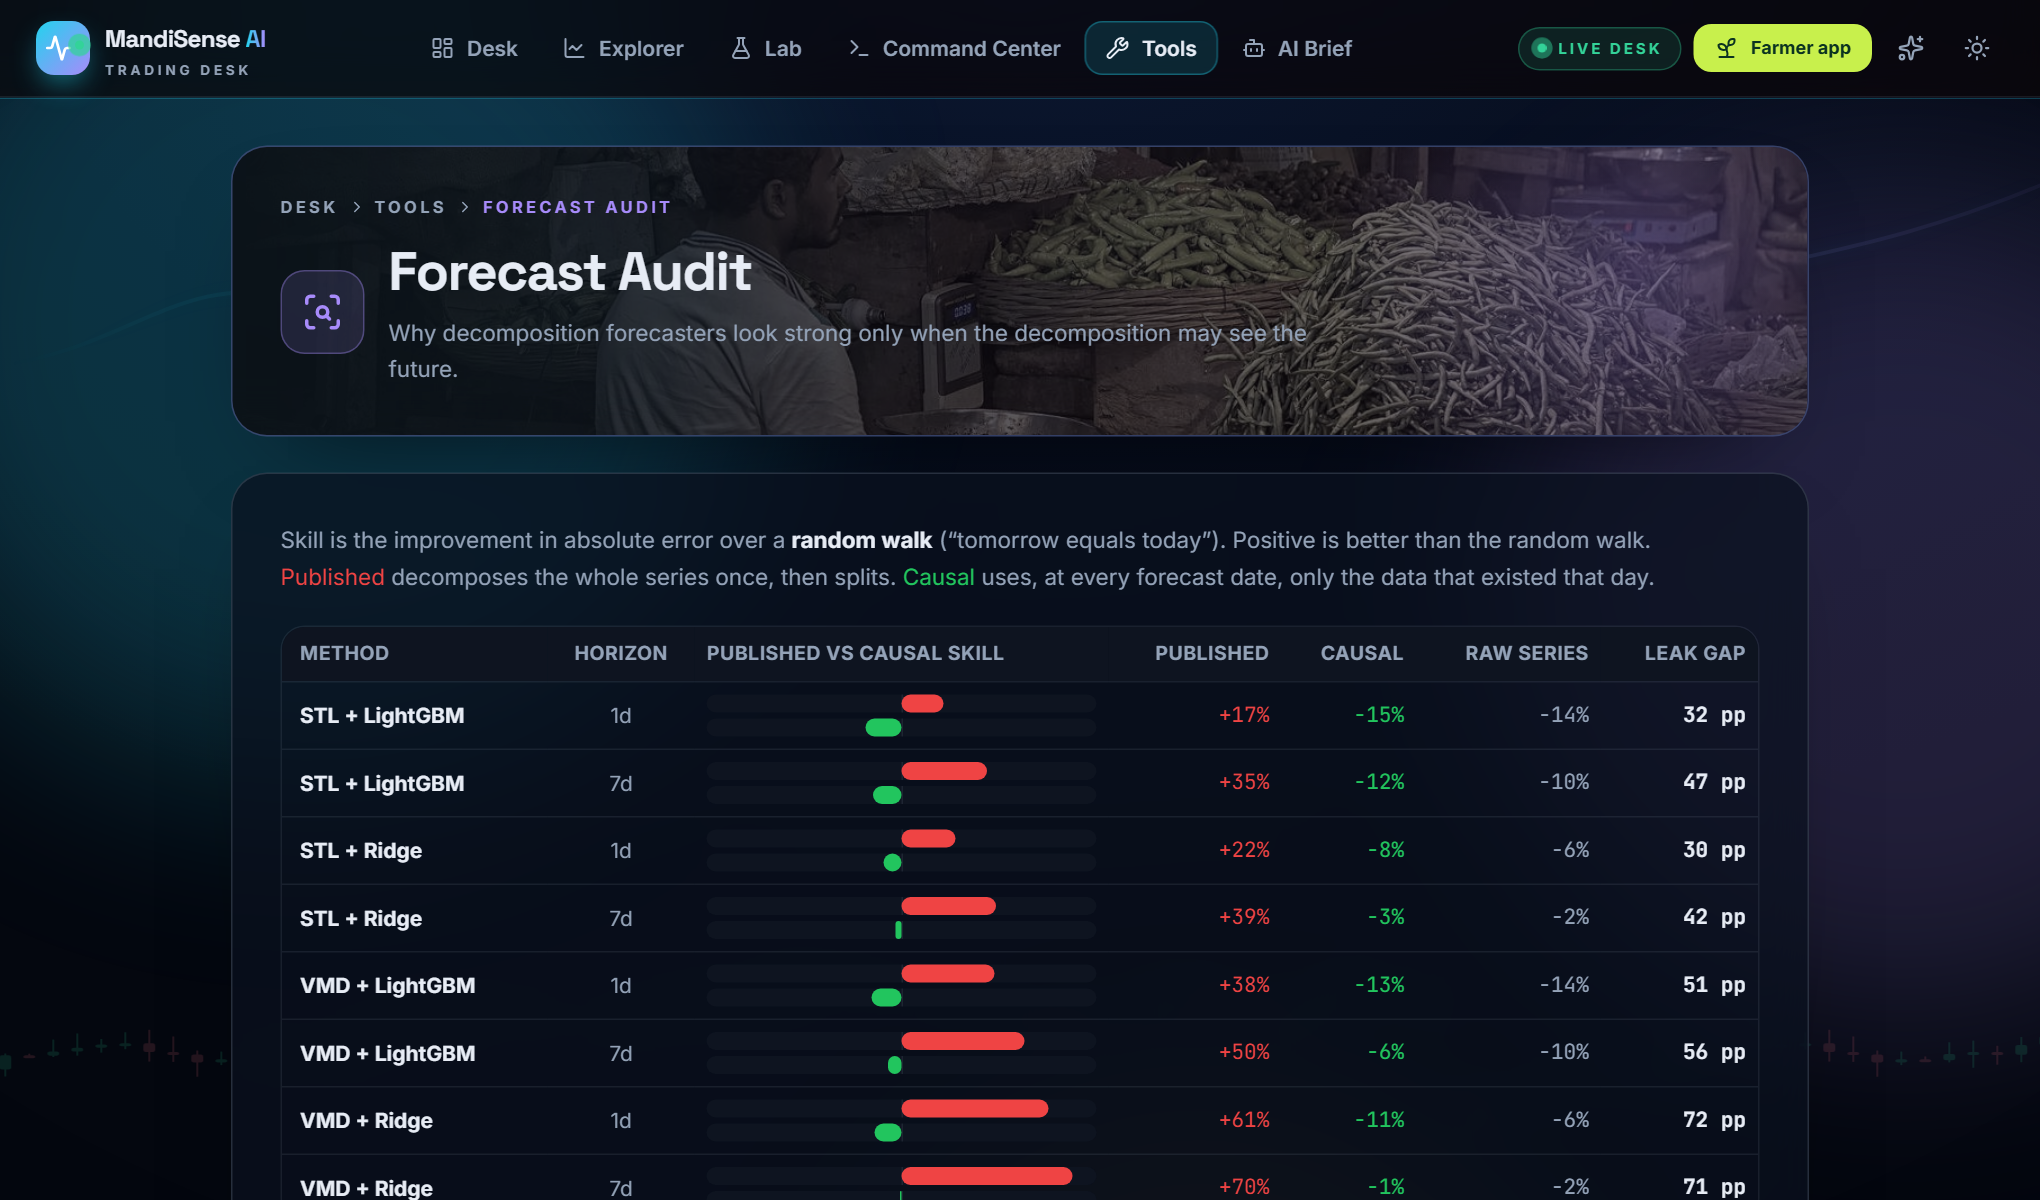
\includegraphics[width=0.93\linewidth]{figures/shot_w_audit.png}}\\[0.5mm]{\footnotesize (b) Forecast audit}
\caption{(a) Floor monitor: how often the revenue floor has held. (b) Forecast audit.}
\label{fig:sc-w-floormon}
\end{figure}

The monitor tracks, day by day, whether realised revenue stayed above the stated floor and shows the running violation rate against its target, so a drift in calibration is visible.

The audit compares each forecaster with the naive predictor on the days it was used and shows where it adds nothing.

\begin{figure}[!t]
\centering
\fbox{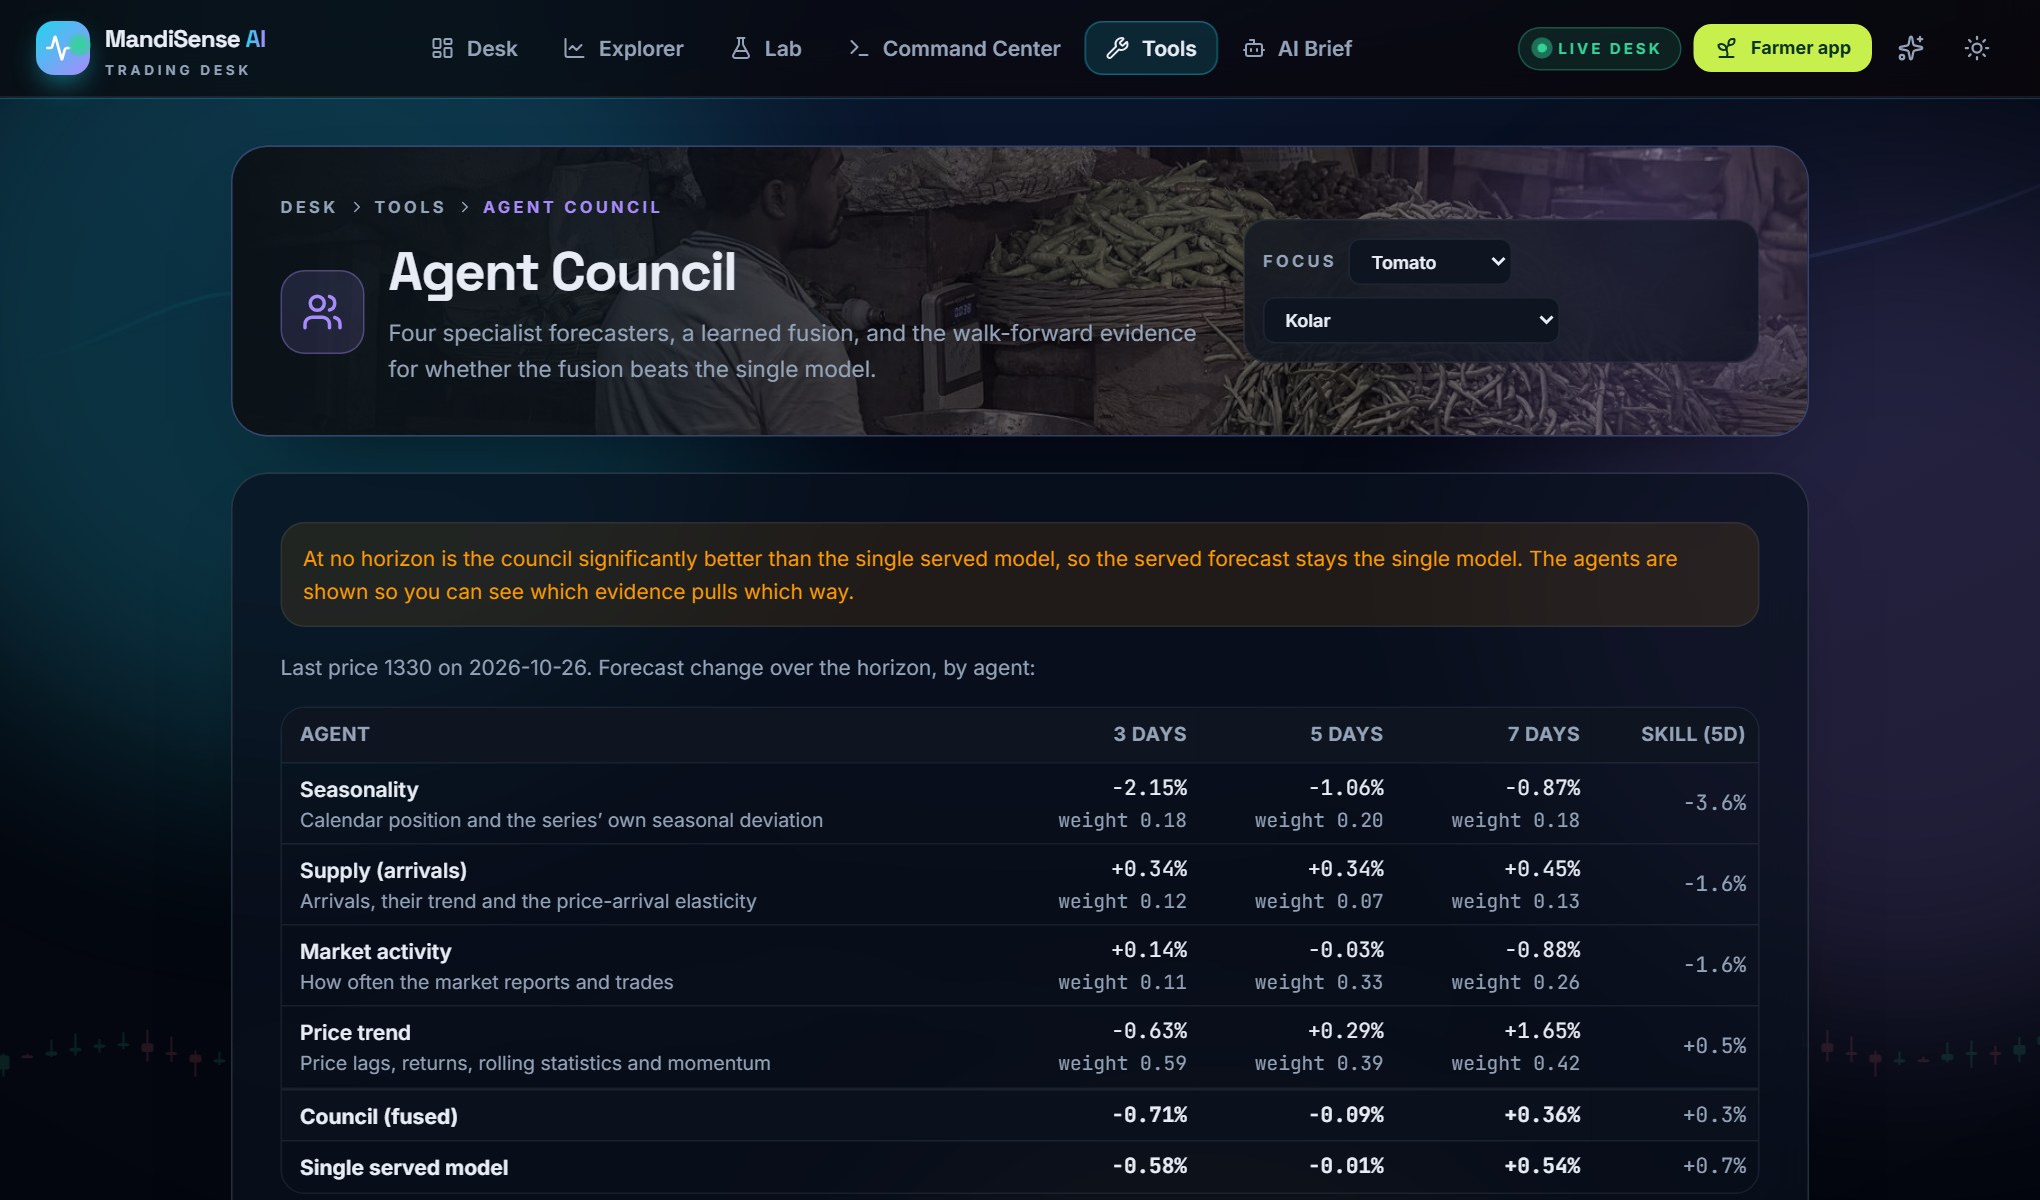
\includegraphics[width=0.93\linewidth]{figures/shot_w_council.png}}\\[0.5mm]{\footnotesize (a) Agent council: specialist forecasters and their weights}
\medskip
\fbox{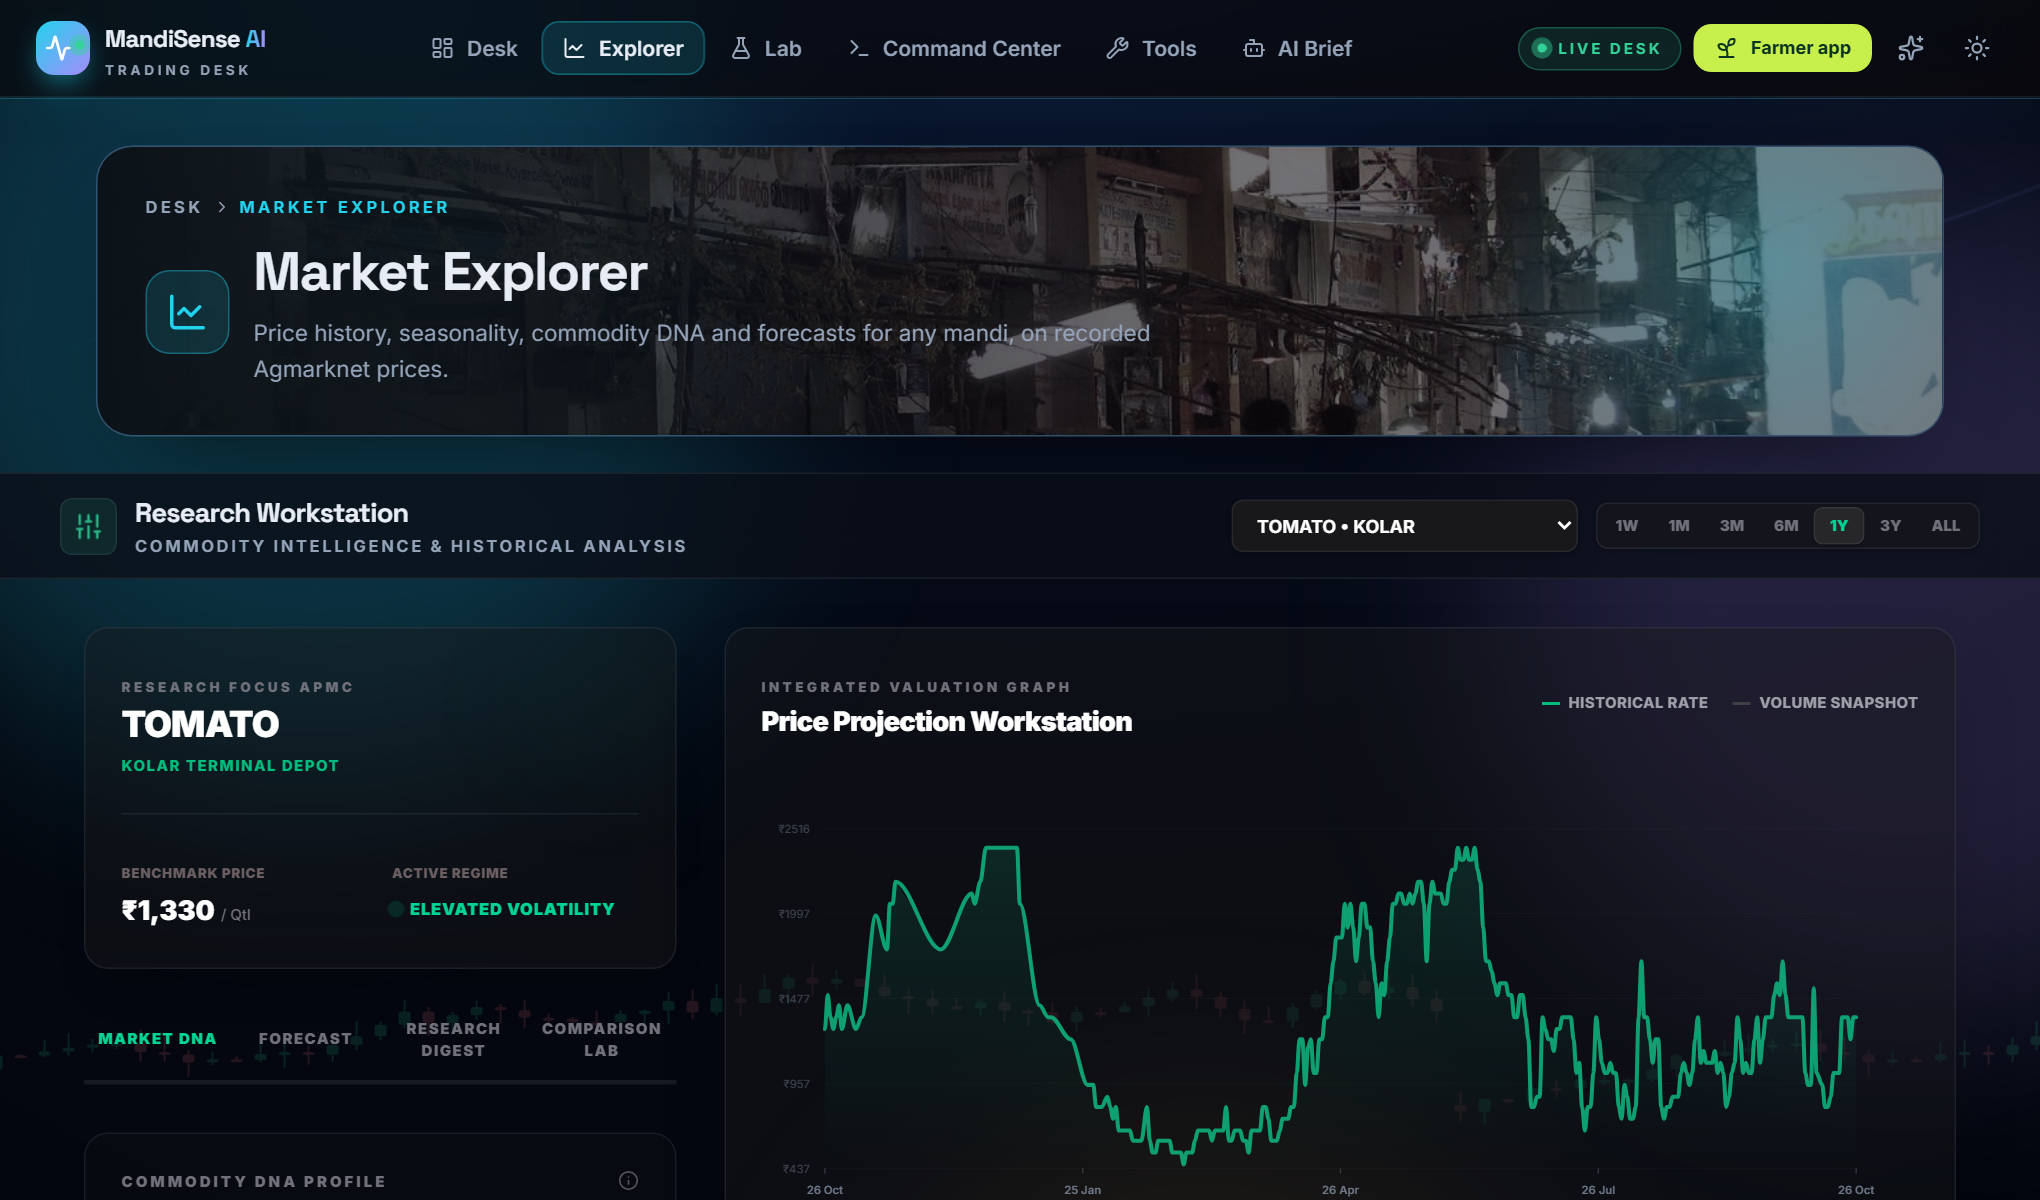
\includegraphics[width=0.93\linewidth]{figures/shot_w_explorer.png}}\\[0.5mm]{\footnotesize (b) Market explorer: any crop, any market, any period}
\caption{(a) Agent council: specialist forecasters and their weights. (b) Market explorer: any crop, any market, any period.}
\label{fig:sc-w-council}
\end{figure}

The council page shows the specialist forecasters and the weight each currently carries, the object of Section~\ref{sec:architecture}.

The explorer lets a user chart raw reported prices and arrivals, with gaps in reporting shown as gaps.

\begin{figure}[!t]
\centering
\fbox{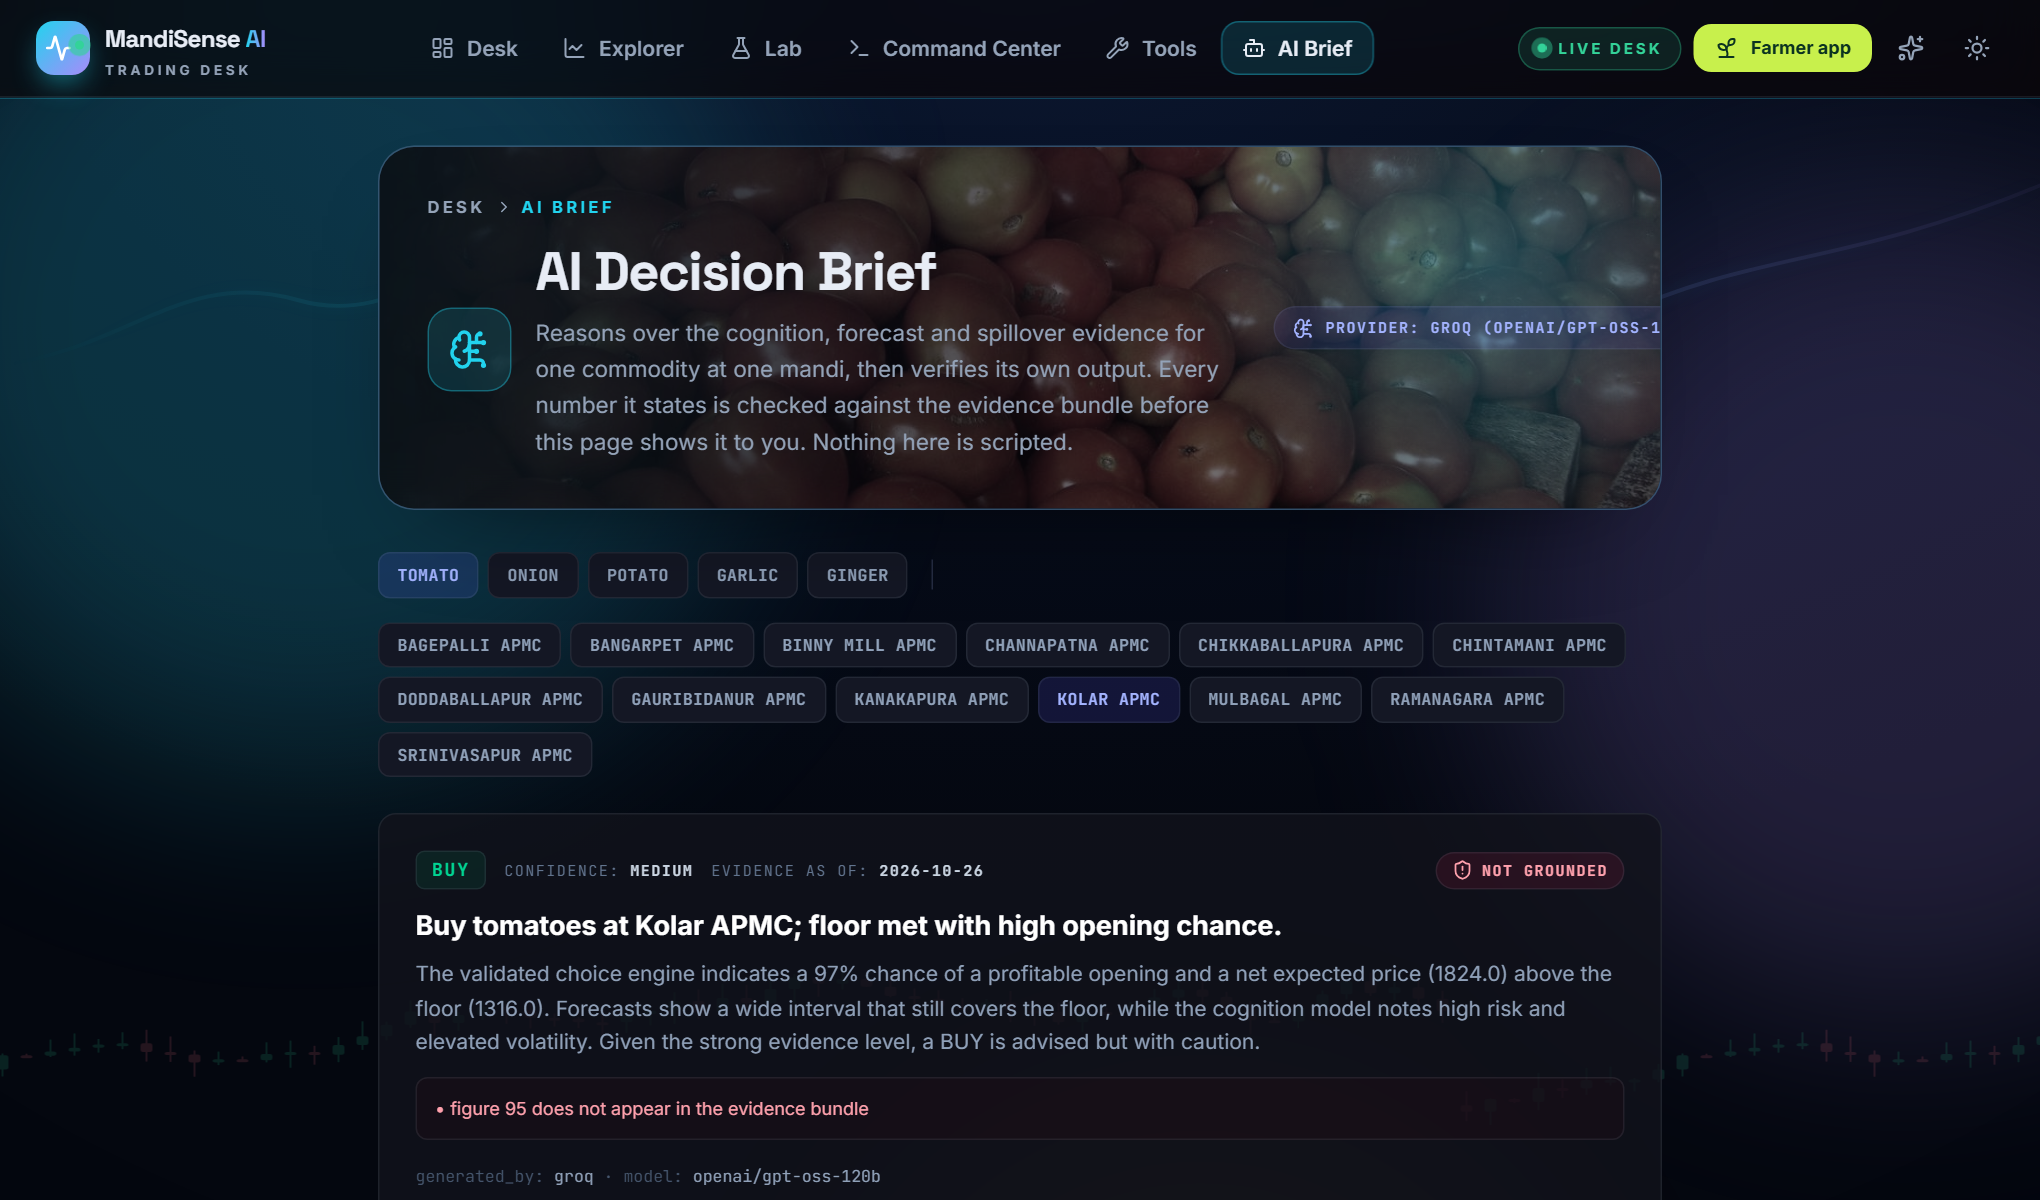
\includegraphics[width=0.93\linewidth]{figures/shot_w_aibrief.png}}\\[0.5mm]{\footnotesize (a) The AI brief: a written summary checked against the evidence}
\medskip
\fbox{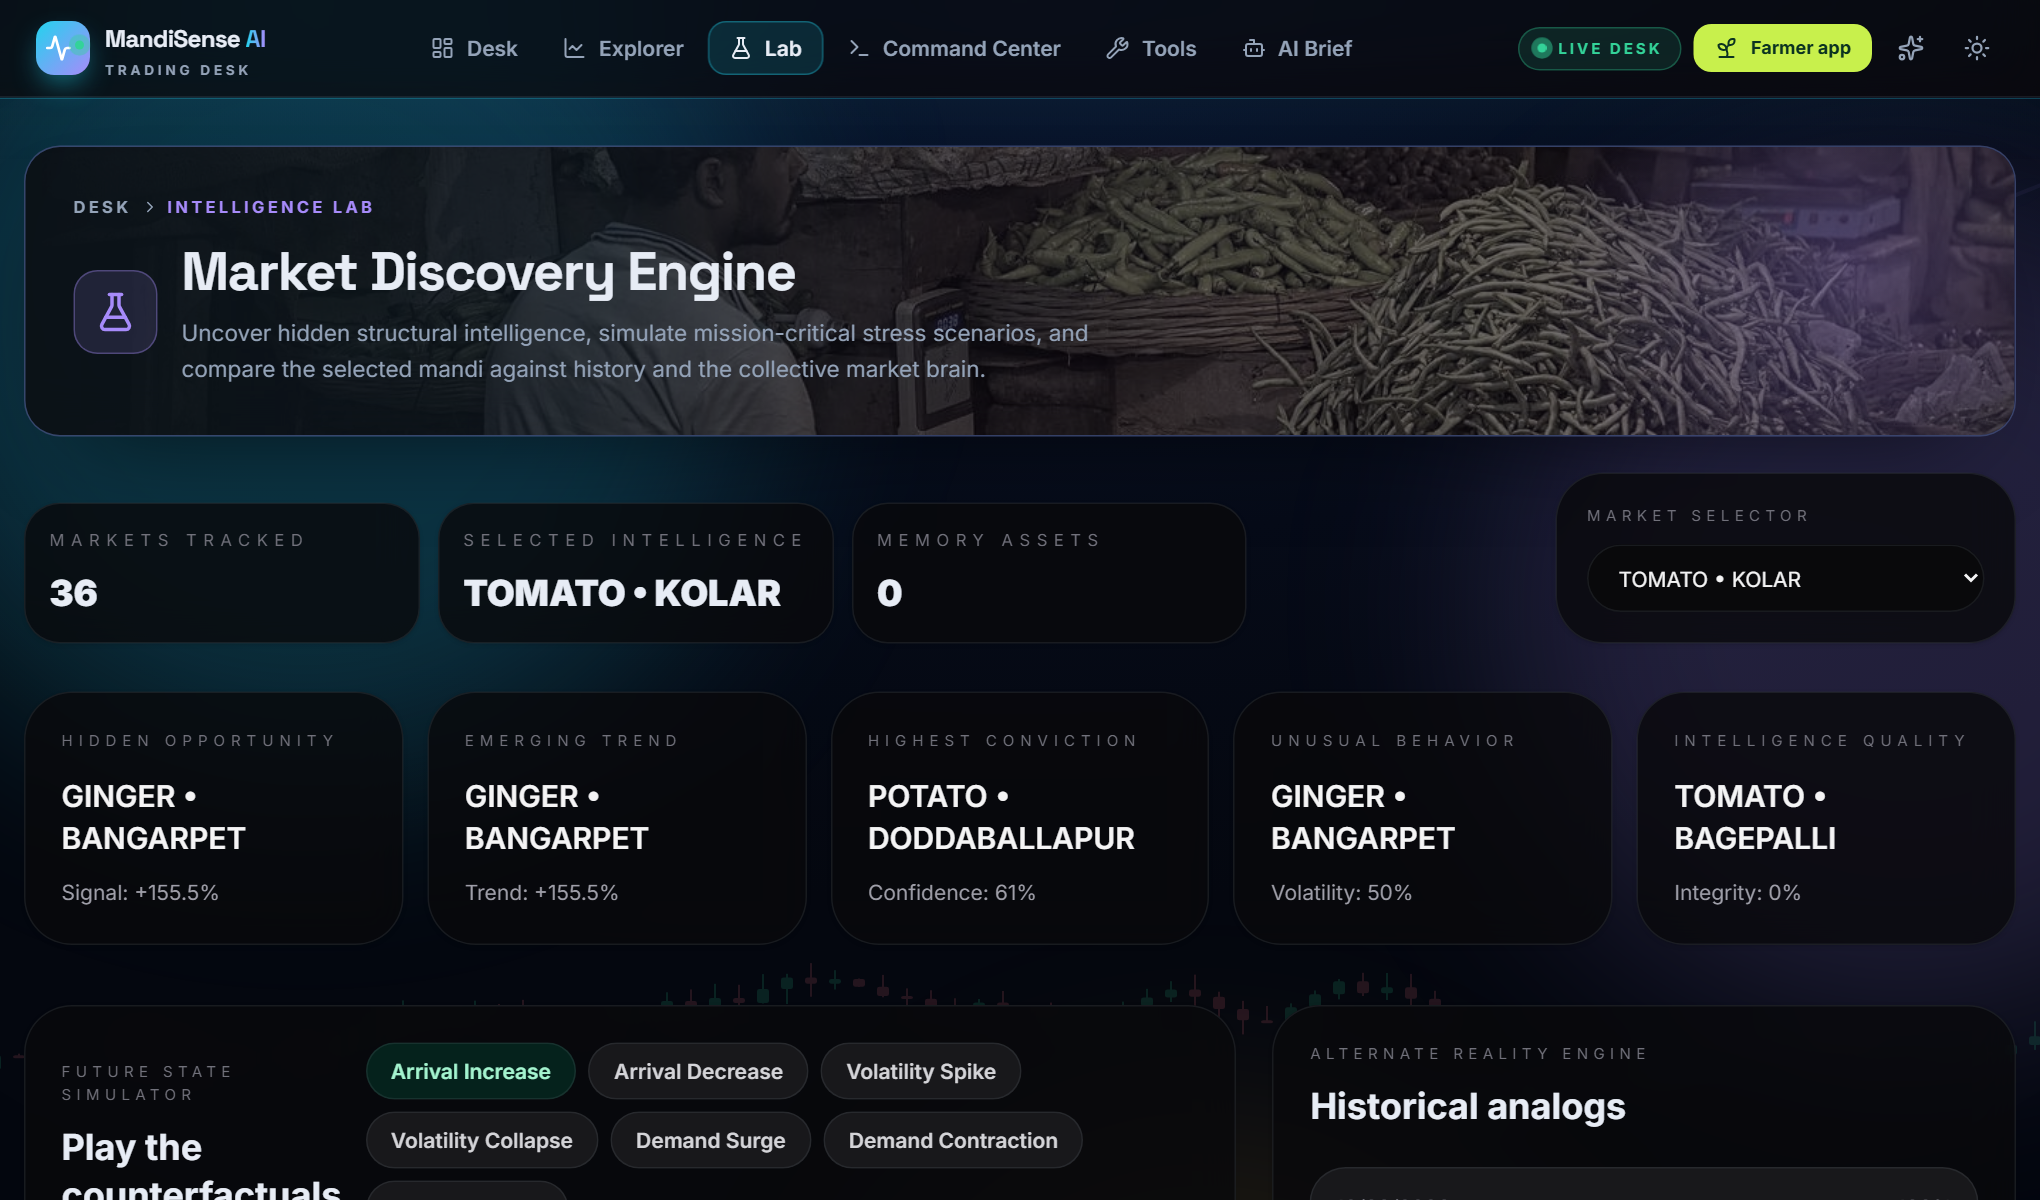
\includegraphics[width=0.93\linewidth]{figures/shot_w_lab.png}}\\[0.5mm]{\footnotesize (b) Intelligence lab: experiment summaries}
\caption{(a) The AI brief: a written summary checked against the evidence. (b) Intelligence lab: experiment summaries.}
\label{fig:sc-w-aibrief}
\end{figure}

The brief is written by the language model of Section~\ref{sec:llm} and every figure in it is checked against the evidence before it is shown. A brief that fails the check is discarded and the page falls back to a plain summary.

The lab page presents the experiment results of Chapter~\ref{ch:results} interactively.

\begin{figure}[!t]
\centering
\fbox{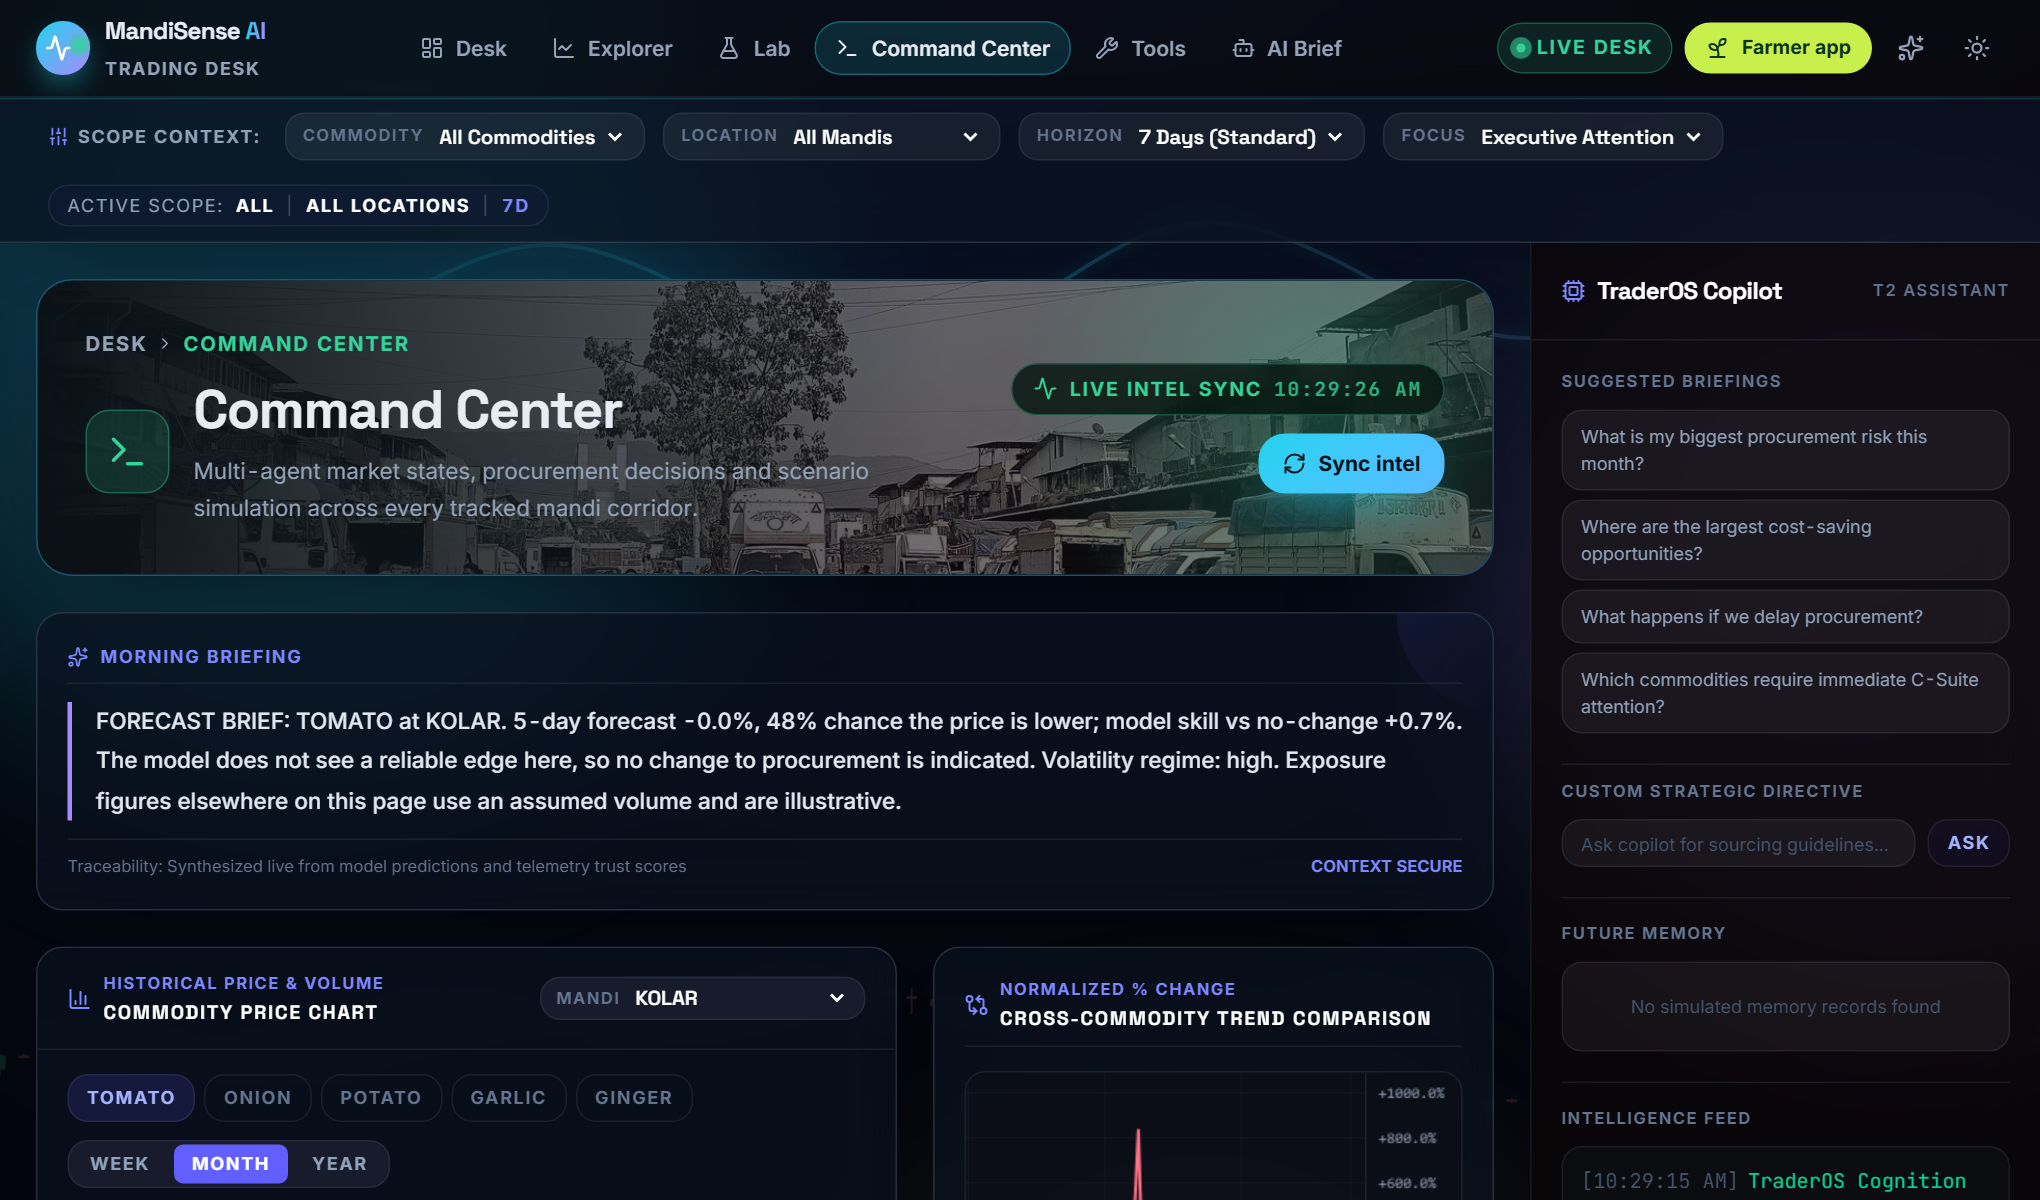
\includegraphics[width=0.93\linewidth]{figures/shot_w_terminal.png}}\\[0.5mm]{\footnotesize (a) Terminal view: dense prices for desk use}
\medskip
\fbox{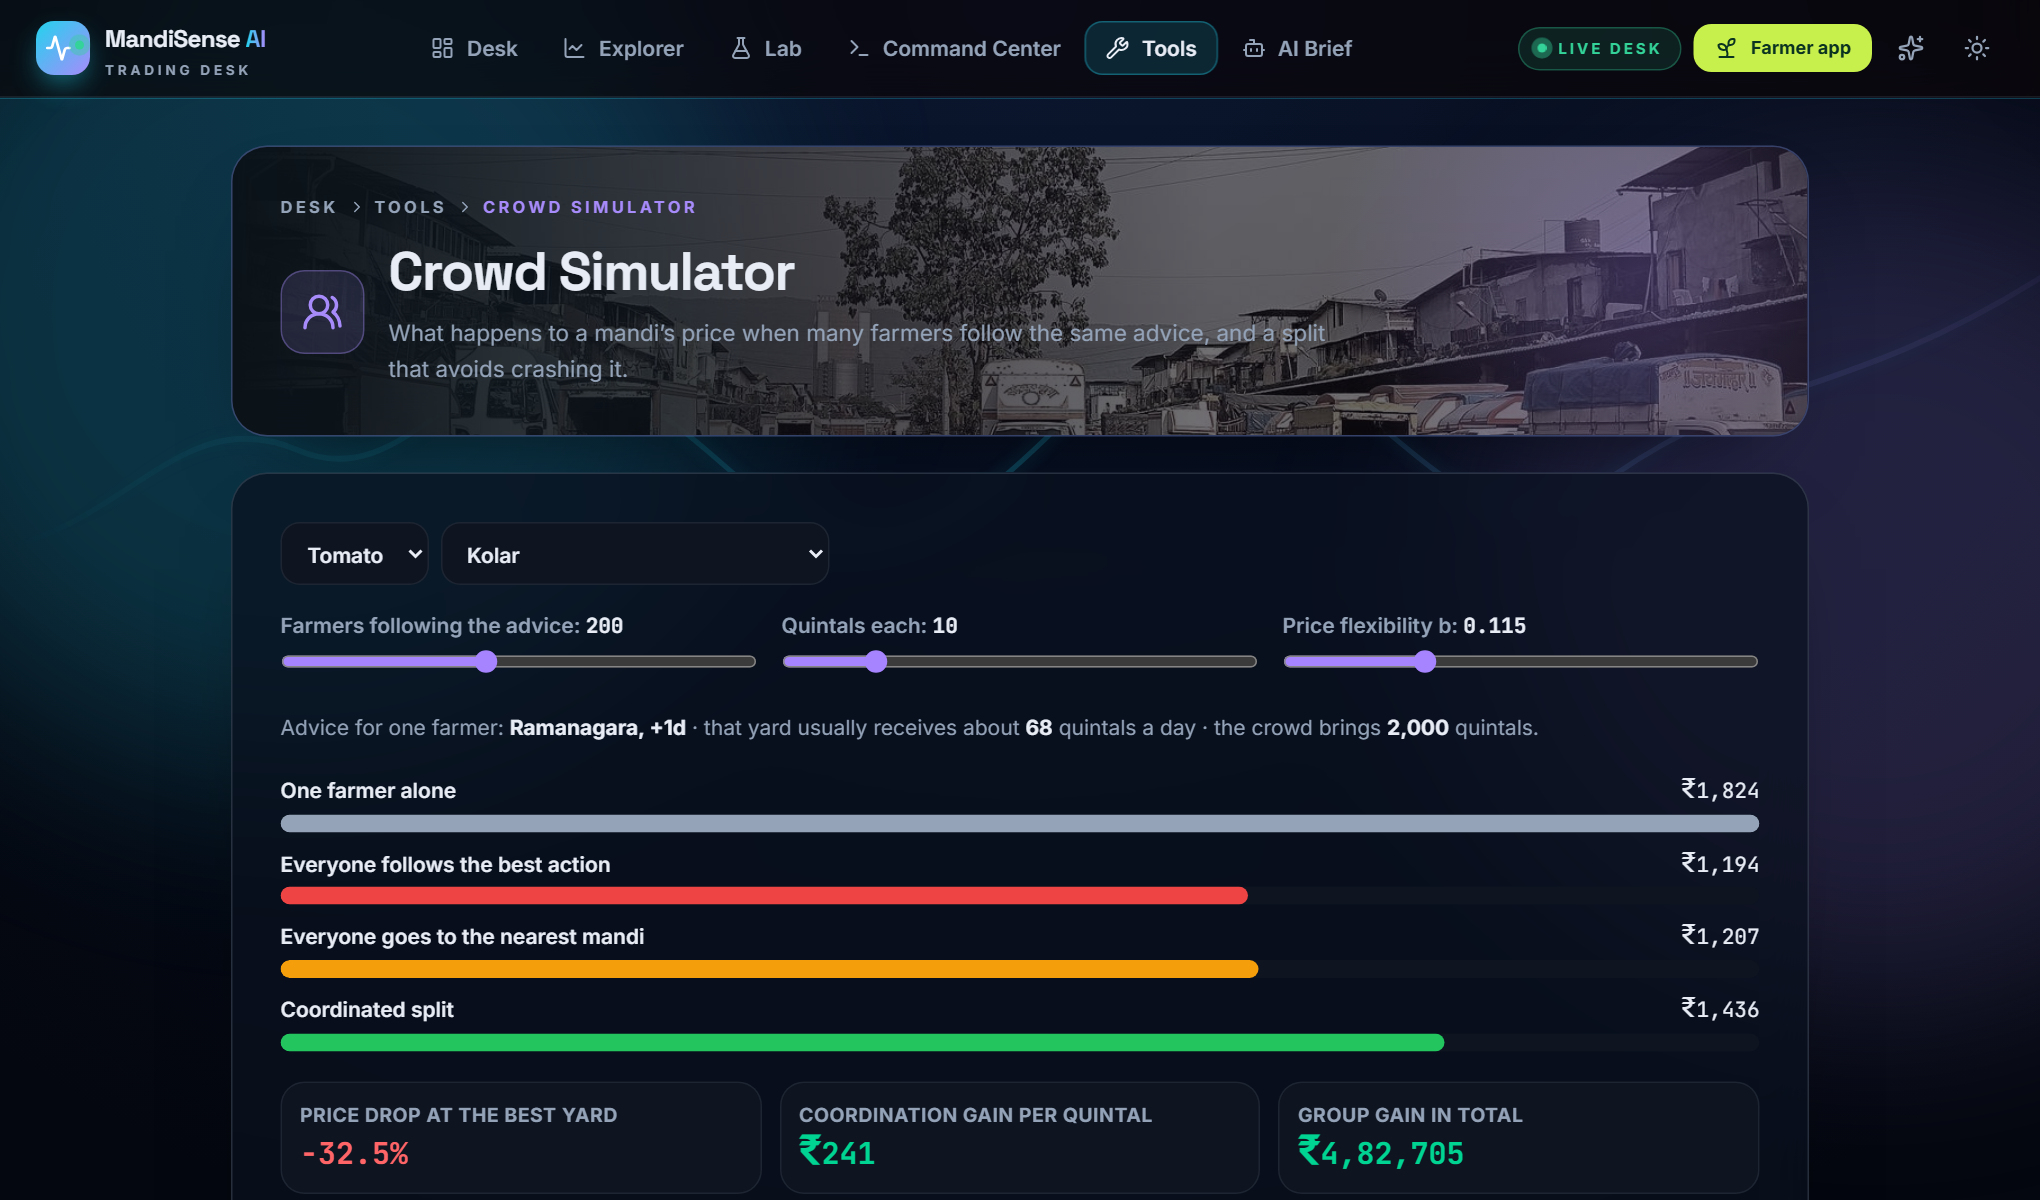
\includegraphics[width=0.93\linewidth]{figures/shot_w_crowd.png}}\\[0.5mm]{\footnotesize (b) Crowd simulator: what happens when many farmers follow the same advice}
\caption{(a) Terminal view: dense prices for desk use. (b) Crowd simulator: what happens when many farmers follow the same advice.}
\label{fig:sc-w-terminal}
\end{figure}

A compact table of the latest price per market, intended to stay open beside other work.

The simulator raises the share of farmers following the advice and shows the net revenue under four policies, using a stated price flexibility (Section~\ref{sec:insight-method}).

\begin{figure}[!t]
\centering
\fbox{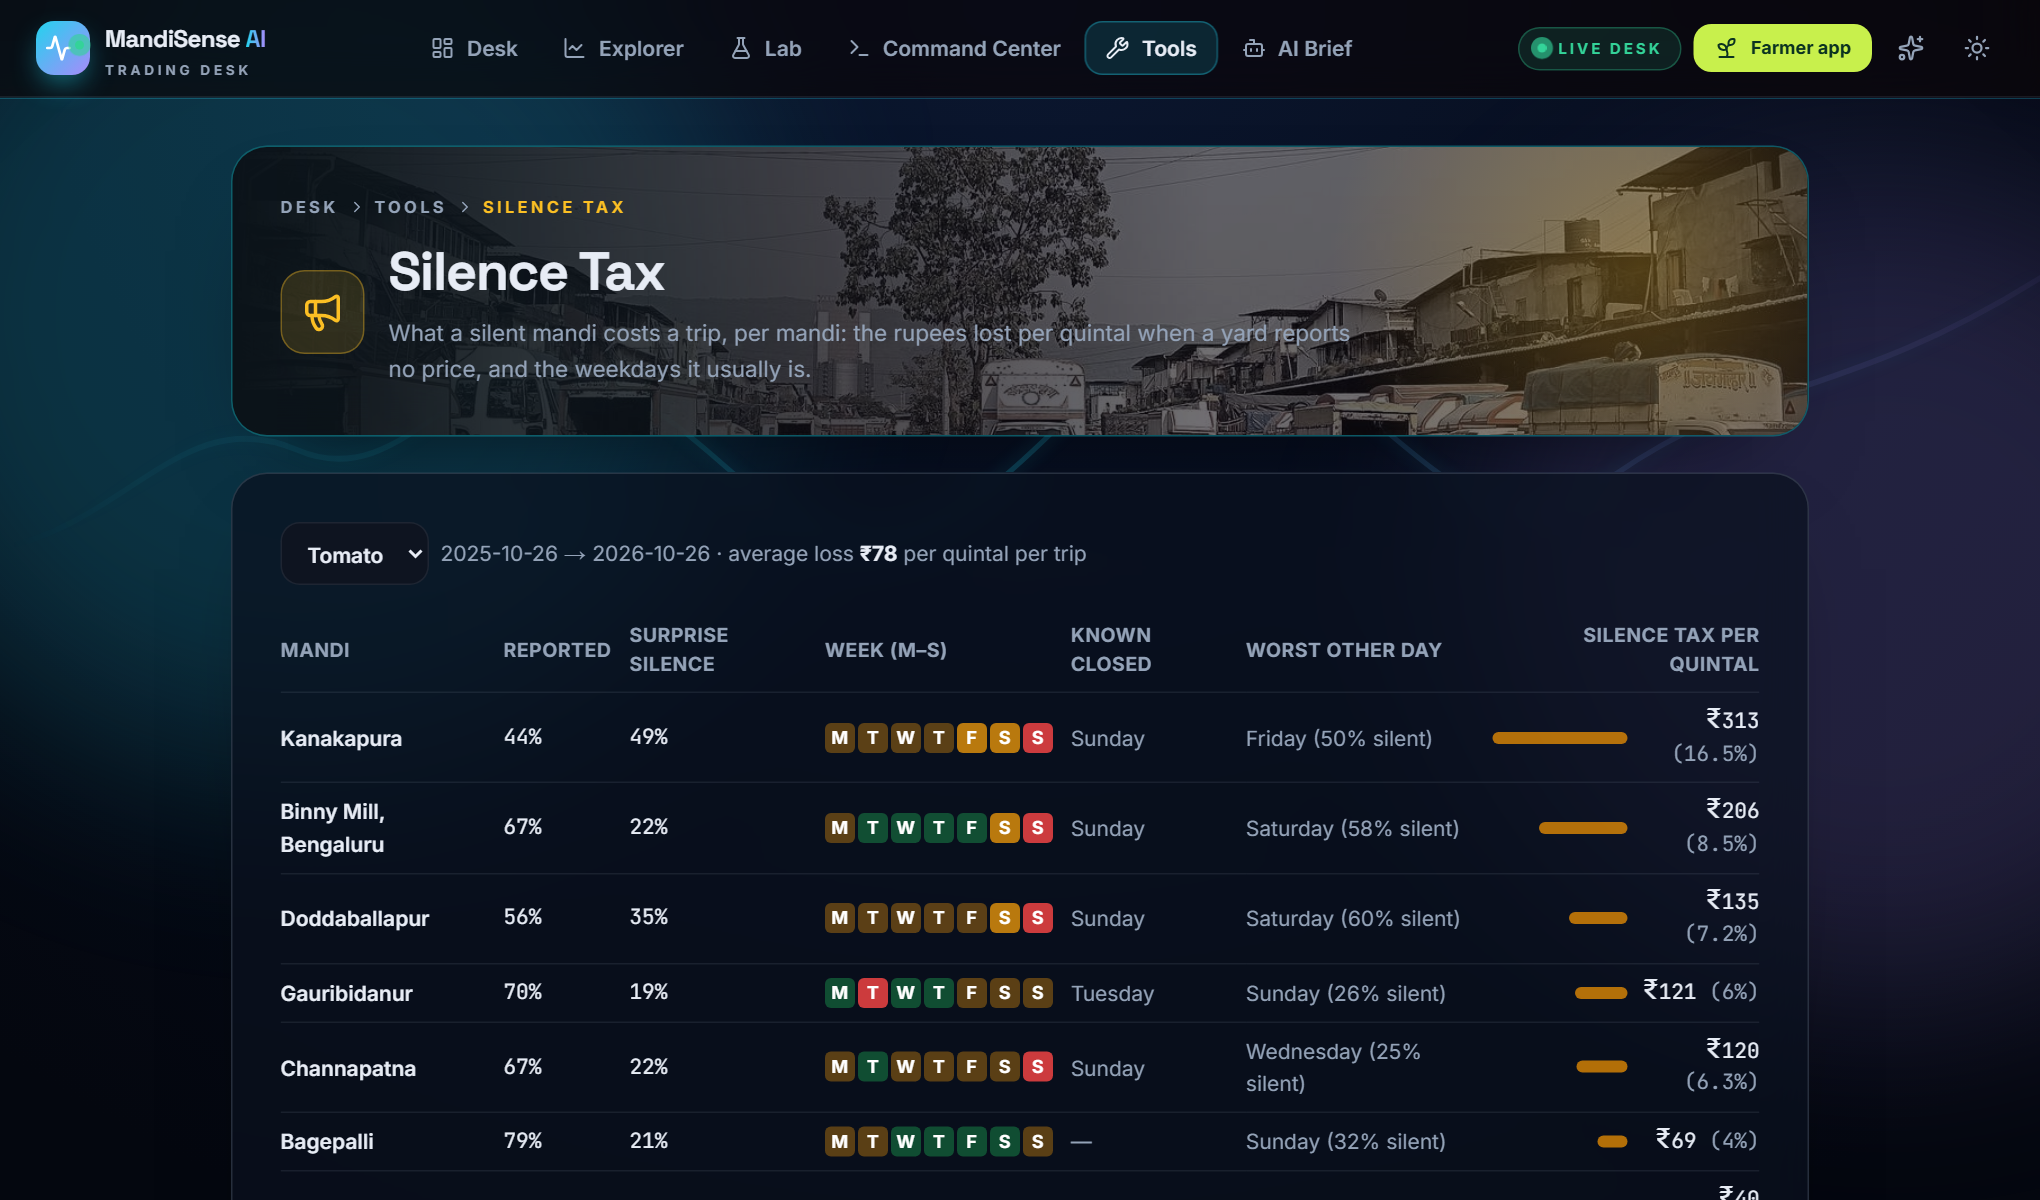
\includegraphics[width=0.93\linewidth]{figures/shot_w_repval.png}}\\[0.5mm]{\footnotesize (a) Reporting value (silence tax): what a market's silence costs}
\medskip
\fbox{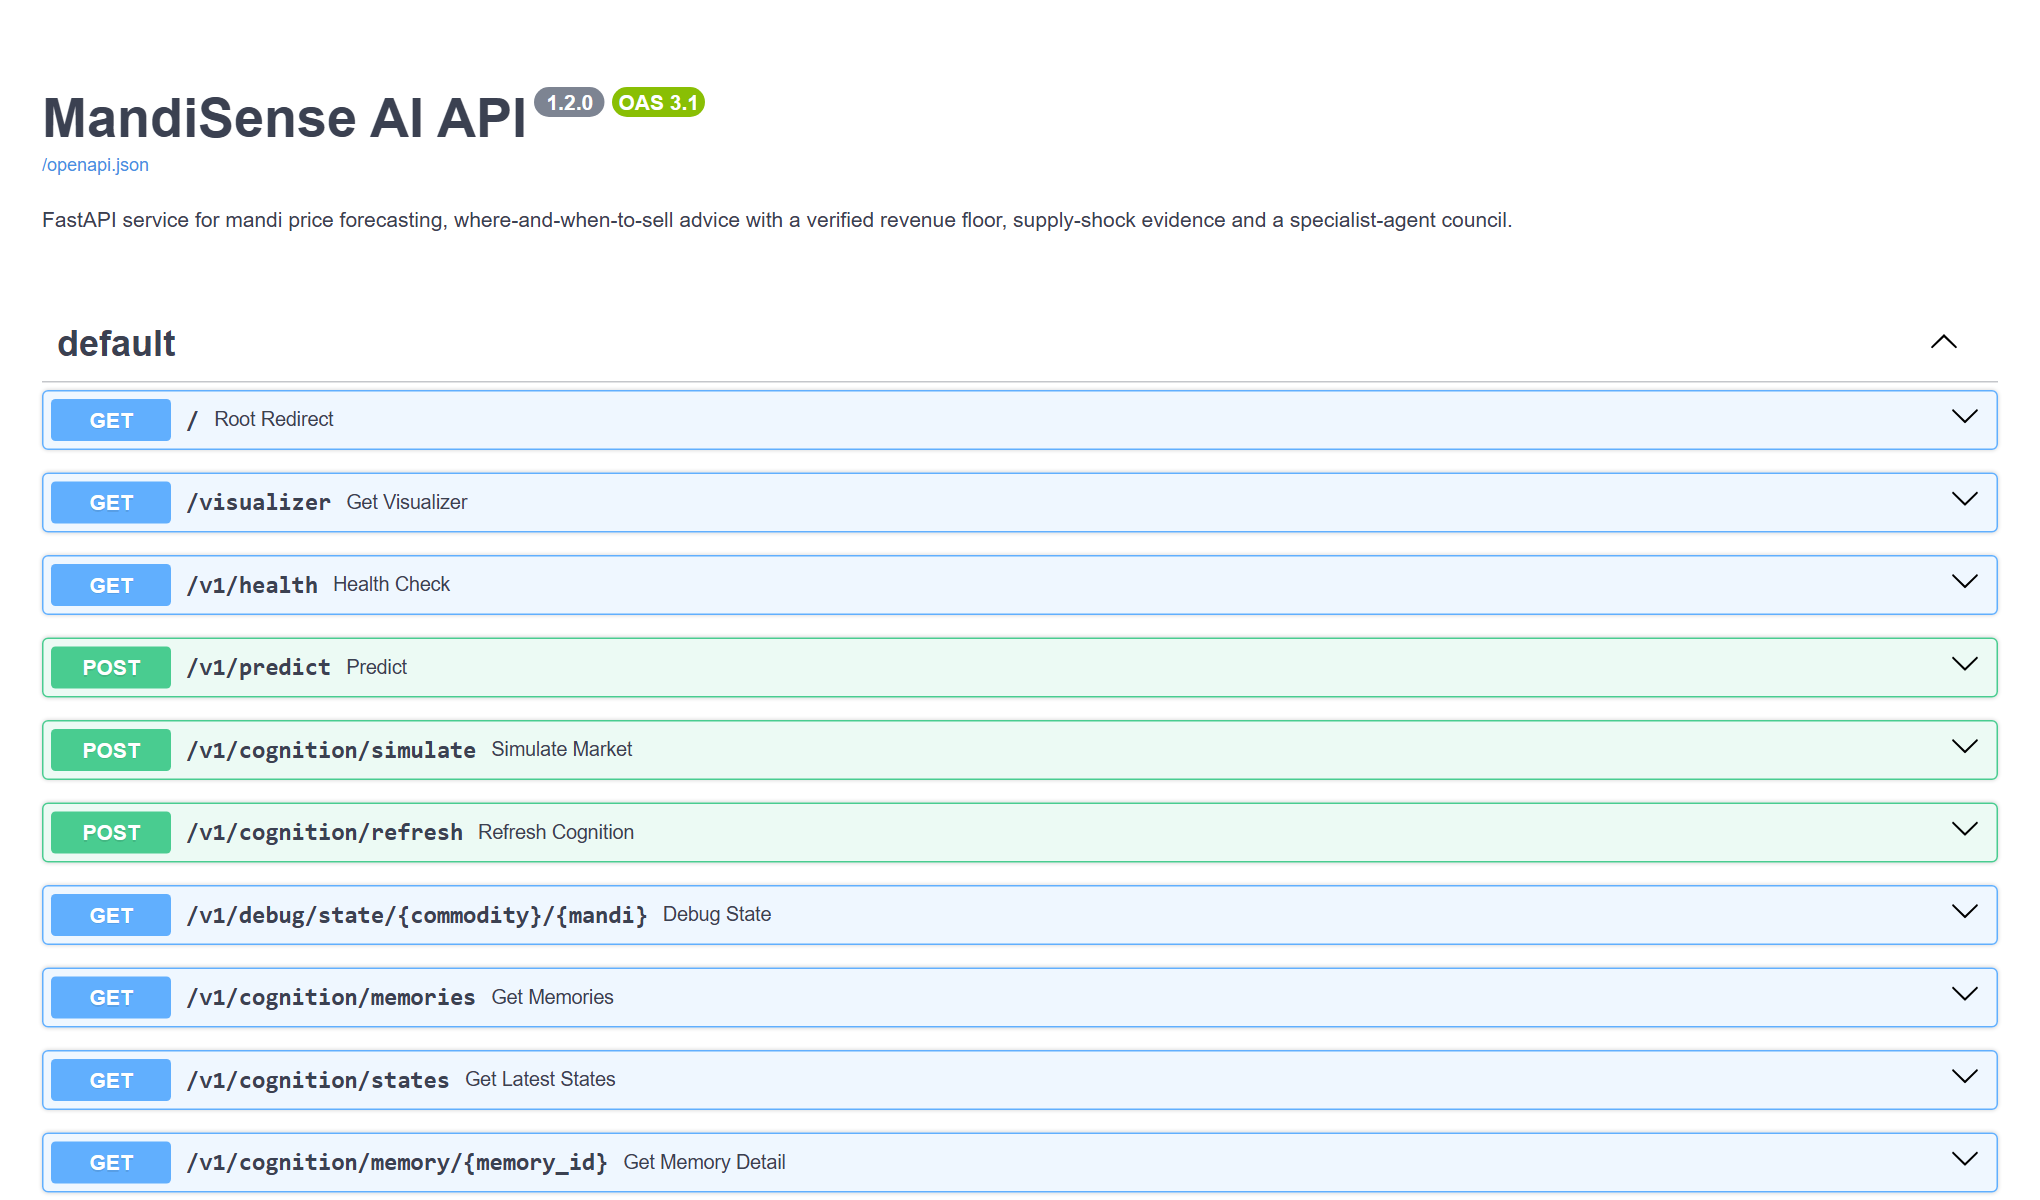
\includegraphics[width=0.93\linewidth]{figures/shot_w_docs.png}}\\[0.5mm]{\footnotesize (b) The interactive API documentation}
\caption{(a) Reporting value (silence tax): what a market's silence costs. (b) The interactive API documentation.}
\label{fig:sc-w-repval}
\end{figure}

The page estimates, per mandi, the revenue lost on days when a market did not report, which is the silence tax of Section~\ref{sec:insight-method}.

Every endpoint is documented automatically from the code, with a form to try it; the service is described in Section~\ref{sec:service-app}.


\section{Testing and Validation}
\label{sec:testing-validation}

\subsection{Strategy}

Testing has four levels. Unit tests check individual functions, including the SPO+ properties (non-negative, zero at the truth, upper bound on regret, respects the offered set, matches brute force) and the conformal quantile. Leakage tests perturb future values and require features to be unchanged, and corrupt not-yet-known outcomes and require the floor to be unchanged. Integration tests exercise the API routers against the real data layer. A results-document test checks that every figure linked from the generated results exists, that no unfilled value leaked, and that headline numbers match the source tables. A continuous-integration workflow runs the Python and web tests on each push.

\subsection{Coverage and outcome}

\begin{table}[!t]
\centering
\caption{Test inventory}
\label{tab:tests}
\small
\begin{tabular}{|l|p{6.4cm}|l|}
\hline
\textbf{Layer} & \textbf{Content} & \textbf{Tool} \\ \hline
Application tests & 669 tests (all passing on 29 October 2026) across engines, API, trader and farmer features, council, shock, spillover, chat, results document, insight features and the digest & pytest \\ \hline
Research tests & Core losses, models, pipeline, leakage; need the separate research environment with PyTorch & pytest \\ \hline
Web tests & 11 copy and registry tests for the three languages and the tool registry & vitest \\ \hline
UI smoke test & 60 checks: every API endpoint and page the application depends on, including the five insight endpoints and the two new trader tools (\texttt{scripts/smoke\_ui.py}) & headless Chrome \\ \hline
Fresh-clone check & Clone, install, run pipeline subset, run tests & manual, repeated \\ \hline
\end{tabular}
\end{table}

\noindent\textbf{Negative outcomes.} The fresh-clone check initially failed (Table~\ref{tab:challenges}); the three research-test modules cannot be collected in the application environment because PyTorch is installed only in the research environment, which is by design but means a single \texttt{pytest} call at the repository root reports three collection errors. The deployment configuration (Docker, Render) is provided but has not been verified end to end, and no claim about a live deployment is made in this thesis.

\chapter{Results and Discussion}
\label{ch:results}

This chapter reports what the experiments found, against the objectives of Chapter~\ref{ch:intro-ref} and the protocol of Section~\ref{sec:setup}. Every table is generated from the experiment artefacts by \texttt{report/build\_assets.py}, so no result was typed by hand. Results that were unfavourable to the proposed ideas are reported with the same prominence as the favourable ones.

\section{Experimental Results}
\label{sec:experimental-results}

\subsection{Setup}
Tomato, onion, potato and ginger were studied, with 963, 511, 569 and 776 scored decision days respectively (Table~\ref{tab:dataset}). Revenue is in rupees per quintal, averaged over decision days and five farmer origins, under the default economics of Section~\ref{sec:formulation}. Brackets give 95\% day-block bootstrap intervals.

\subsection{Decision quality}

Table~\ref{tab:decision} gives mean realised revenue. In every crop the ordering is the same: nearest-mandi selling is worst; the highest price yesterday, the random walk and the boosted model trained on observed prices are close to each other; and the two models trained on realised outcomes are best. For tomato, the realised-outcome LightGBM earned Rs~2,156 per quintal against Rs~2,021 for the highest price yesterday and Rs~1,600 for the nearest mandi, with a hindsight oracle at Rs~2,570.

\begin{table}[!b]
\centering
\caption{Mean realised net revenue (Rs per quintal) with 95\% intervals; oracle shown without interval}
\label{tab:decision}
\gentable{tab_decision}
\end{table}

\begin{table}[!t]
\centering
\caption{Share of the nearest-mandi-to-oracle gap closed, and share of recommendations sent to a silent market}
\label{tab:gap}
\gentable{tab_gap}
\end{table}

\begin{figure}[!t]
\centering
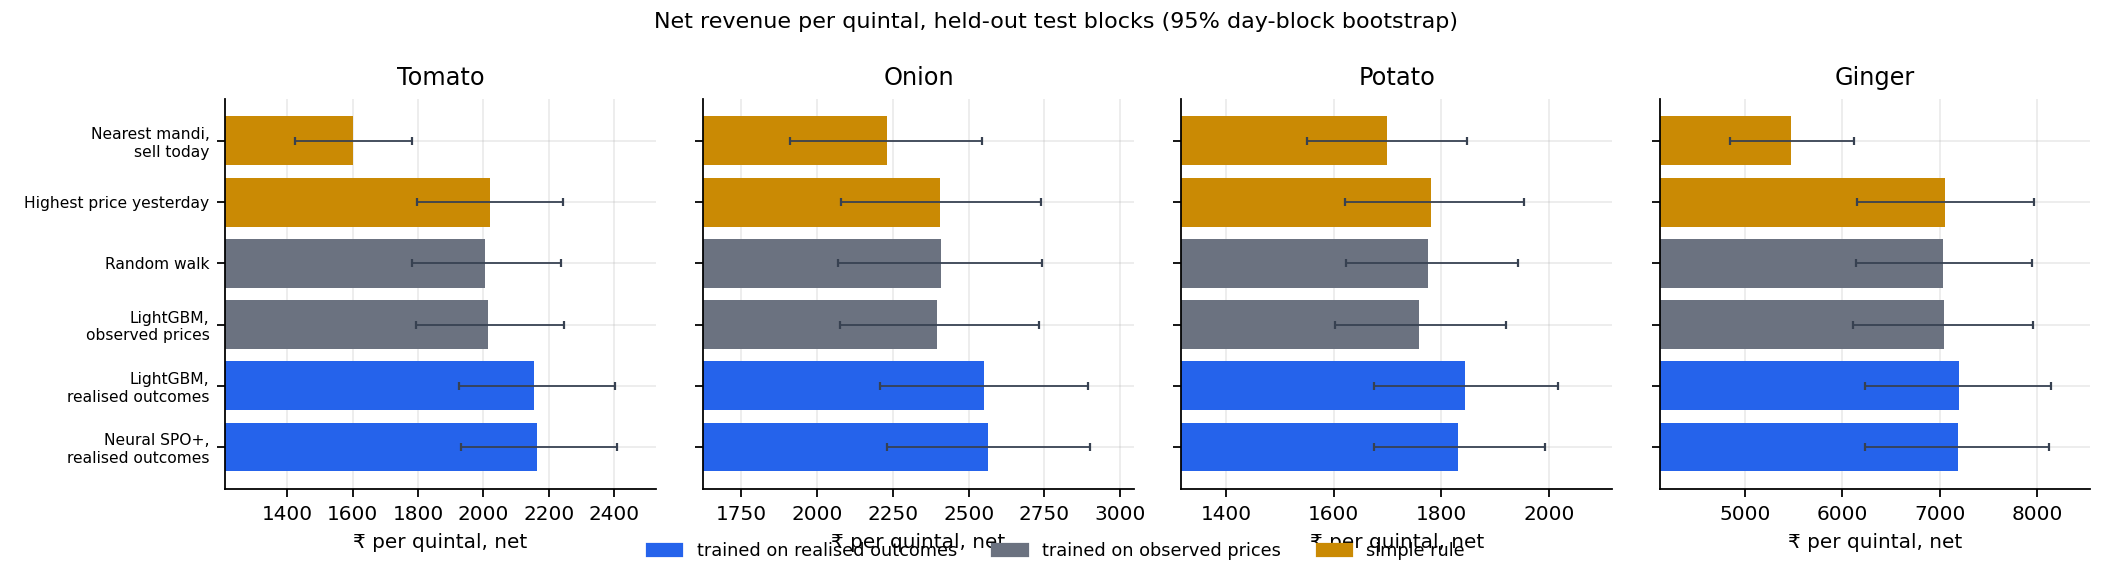
\includegraphics[width=0.85\textwidth,height=7.2cm,keepaspectratio]{figures/fig_decision_revenue.png}
\caption{Mean realised revenue by method and crop with bootstrap intervals.}
\label{fig:decision-revenue}
\end{figure}

\noindent Table~\ref{tab:gap} shows the mechanism. Models trained on observed prices sent between 12\% (ginger) and 43\% (onion) of recommendations to a market that was silent that day; the same learner trained on realised outcomes cut this by half or more (to 5--21\%). A model that never sees a silent cell cannot learn to avoid one.

\section{Performance Evaluation}
\label{sec:performance-evaluation}

\subsection{What improved decisions: the labels}
\label{sec:effects}

Table~\ref{tab:effect} isolates the two candidate causes of better decisions. Changing the \emph{labels} from observed price to realised revenue, with the same LightGBM learner, reduced regret by Rs~\LabelEffectTomato{} (tomato), \LabelEffectOnion{} (onion), \LabelEffectPotato{} (potato) and \LabelEffectGinger{} (ginger) per quintal, with Holm-adjusted $p<0.002$ in all four. The neural model showed the same effect for tomato (Rs~\LabelEffectNeural{}, interval \LabelEffectNeuralCI{}). Changing the \emph{loss} from squared error to SPO+, with labels held fixed, produced point estimates between Rs~$-66$ and $+1$ but none was reliably different from zero (Holm $p$ from 0.17 to 0.95). The honest reading is that the gain comes from learning on what the farmer actually received, and that this thesis did not find evidence for the decision-focused loss on top of it. This contradicts the expectation that SPO+ would help~\cite{elmachtoub2022} and is consistent with the finding that its benefit depends on the problem~\cite{mandi2024}.

\begin{table}[!t]
\centering
\caption{Effect of realised-outcome labels on regret (LightGBM), and of SPO+ over squared error (neural, same labels)}
\label{tab:effect}
\gentable{tab_effect}
\end{table}

\begin{figure}[!t]
\centering
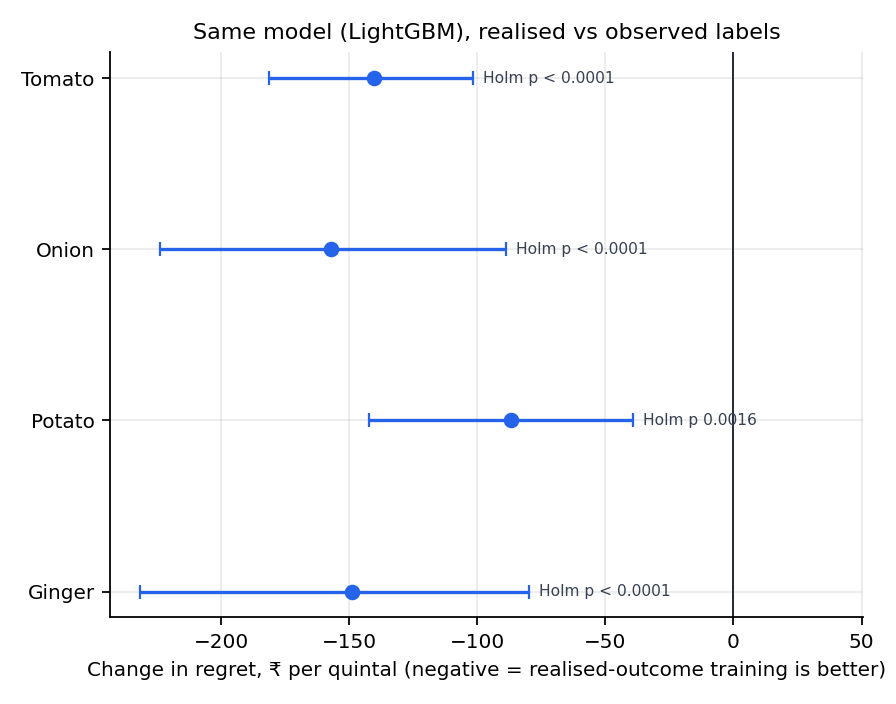
\includegraphics[width=0.85\textwidth,height=7.2cm,keepaspectratio]{figures/fig_label_effect.png}
\caption{Change in regret from realised-outcome labels, by crop, with intervals.}
\label{fig:label-effect}
\end{figure}

The model confidence set at the 10\% level retained only models trained on realised outcomes in every crop (for tomato seven specifications; for onion, potato and ginger the boosted and neural models on realised labels, with and without SPO+). No model trained on observed prices survived in any crop.

\subsection{Revenue floors}
\label{sec:floor-results}

Table~\ref{tab:floor} gives the share of days on which realised revenue fell below the stated floor. Adaptive floors were close to their targets: at a 10\% nominal level the violation rate was 9.0\% (tomato), 6.3\% (onion), 6.9\% (potato) and 10.5\% (ginger), and at 5\% and 20\% they stayed at or below the target in every crop except for marginal excesses at the 20\% level (21.3\% for tomato, 20.4\% for ginger). The static quantile was conservative, and the naive Gaussian floor, which assumes normal errors, failed badly in three crops (26--35\% violations against a 10\% target) and came closest in ginger (11.9\%). Objective 4 asked for a violation rate within two points of 10\%; this was met for tomato and ginger. For onion and potato the floors were more cautious than needed, which is the safe direction, and the objective as written was not met there.

\begin{table}[!t]
\centering
\caption{Floor violation rate (\%) on test days, served LightGBM on realised outcomes}
\label{tab:floor}
\gentable{tab_floor}
\end{table}

\begin{figure}[!t]
\centering
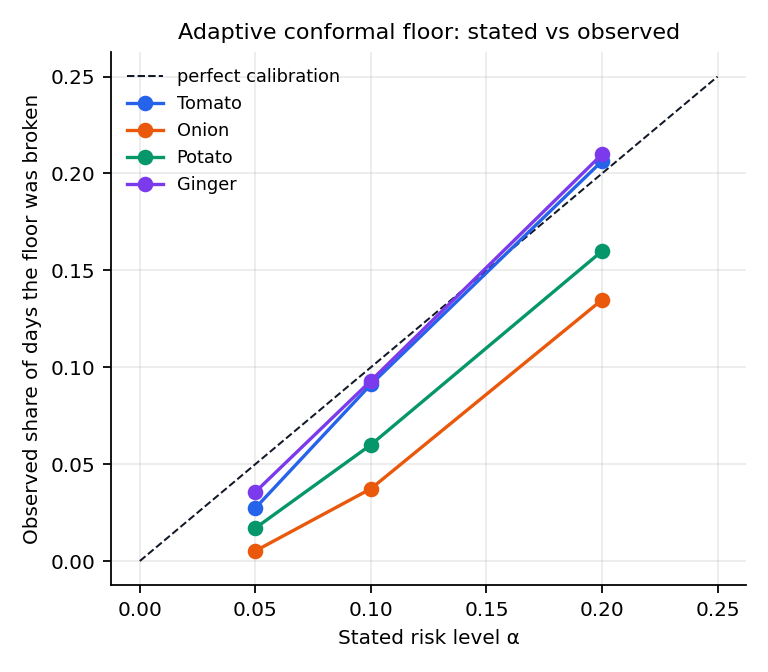
\includegraphics[width=0.85\textwidth,height=7.2cm,keepaspectratio]{figures/fig_floor_calibration.png}
\caption{Calibration of floors: observed violation against nominal level.}
\label{fig:floor-cal}
\end{figure}

\subsection{The served engines}

The engines served by the application were back-tested on the last 330 days, using only information available on each day (Table~\ref{tab:engine}). For tomato the advice earned Rs~\EngineTomatoGain{} per quintal more than the highest price yesterday, and Rs~\EngineTomatoNearest{} more than selling at the nearest mandi; ginger and onion were also significantly better than the strongest heuristic. For potato the gain over the highest price yesterday (Rs~15, interval $-38$ to $+60$) cannot be distinguished from zero, and the system labels the evidence for potato ``limited'' accordingly. Garlic is refused rather than served.

\begin{table}[!t]
\centering
\caption{Back-test of the served engines, last 330 days}
\label{tab:engine}
\gentable{tab_engine}
\end{table}

\begin{figure}[!t]
\centering
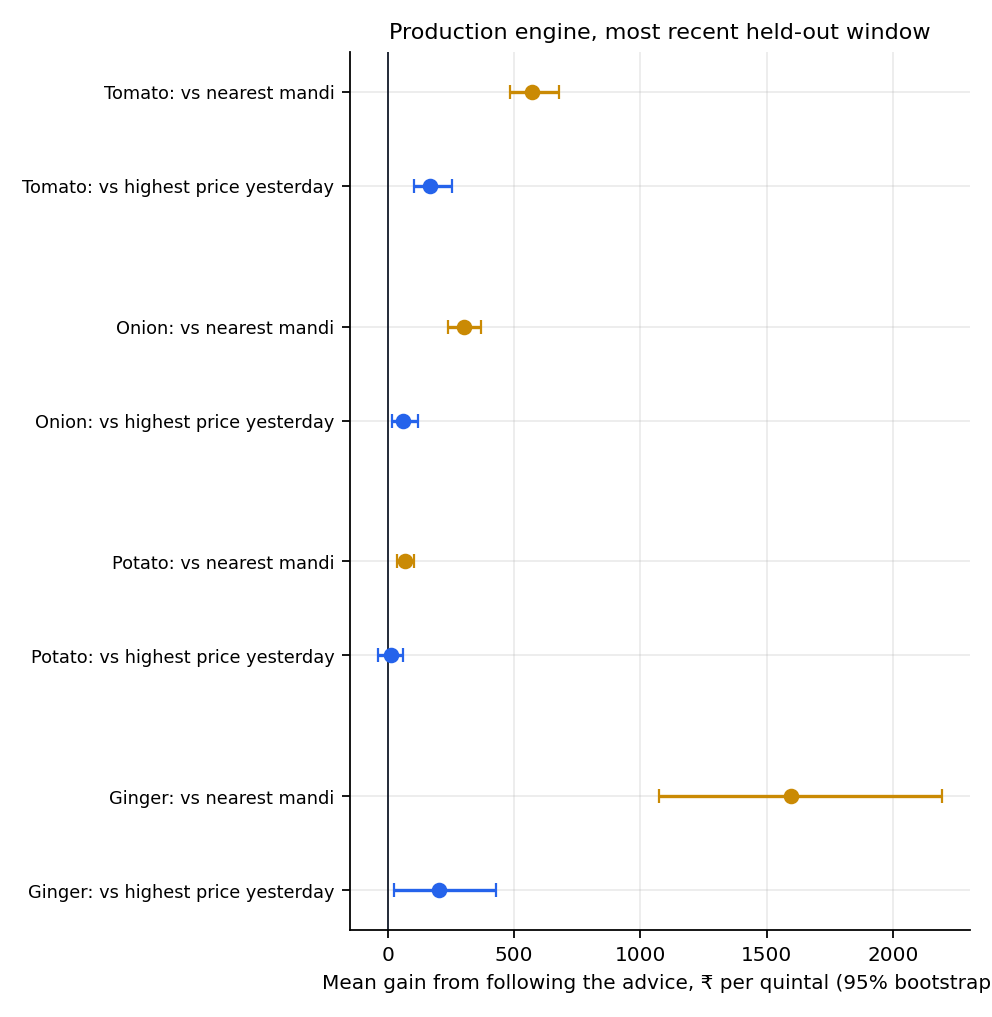
\includegraphics[width=0.85\textwidth,height=7.2cm,keepaspectratio]{figures/fig_engine_backtest.png}
\caption{Daily-backtest gain of the served advice over the two heuristic rules.}
\label{fig:engine-bt}
\end{figure}

\subsection{Price forecasts and the specialist council}

District-level forecasts of the modal price are served only where they beat no change (Table~\ref{tab:district}). The 3-, 5- and 7-day horizons showed skill of 3.0--4.0\% against no change, with direction right on 60--62\% of occasions and 90\% bands that covered 89.8\% of outcomes, at the cost of wide bands (62--75\% of the price). The 1-day horizon was not served: its skill of 0.2\% is not distinguishable from no change.

\begin{table}[!t]
\centering
\caption{District forecast report: skill against no change, direction, band coverage, and whether the horizon is served}
\label{tab:district}
\gentable{tab_district}
\end{table}

Table~\ref{tab:forecast} compares a single model, a linear stack and the specialist council on market-level forecasts. The council improved on the single model in only one of four folds at 3 and 5 days and in none at 7 days, and its average skill (+0.2 to +0.4\%) did not exceed the single model's (+0.6 to +0.8\%). The council was therefore not promoted to the served system; it is retained as an inspectable diagnostic. Table~\ref{tab:council} shows the weights: the trend agent carried most weight and the seasonal agent, alone, was worse than no change.

\begin{table}[!t]
\centering
\caption{Skill against no change: single model, linear stack (ElasticNet), equal-weight agents and weighted council. ``Folds won'' counts the folds in which the single model beat no change}
\label{tab:forecast}
\gentable{tab_forecast}
\end{table}

\begin{table}[!t]
\centering
\caption{Skill and mean weight of each specialist agent}
\label{tab:council}
\gentable{tab_council}
\end{table}

\begin{figure}[!t]
\centering
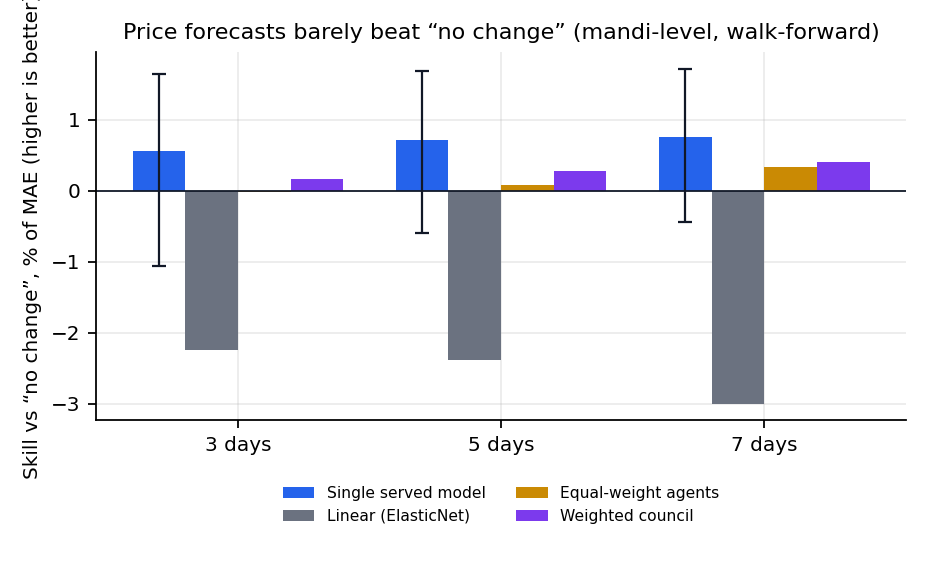
\includegraphics[width=0.85\textwidth,height=7.2cm,keepaspectratio]{figures/fig_forecast_skill.png}
\caption{Forecast skill against no change across horizons.}
\label{fig:forecast-skill}
\end{figure}

\subsection{Explaining and stress-testing the advice}
\label{sec:insight-results}

Table~\ref{tab:breakdown} is the breakdown for tomato at Kolar with 10 quintals: its parts add up to the served net revenue (a test requires it). The advice, \AdvMandi{} after \AdvDays{} day, nets Rs~\AdvNet{} per quintal against Rs~\NearNet{} at the nearest mandi: the price it expects is Rs~776 higher, and that outweighs its extra transport (Rs~94) and spoilage (Rs~60). Table~\ref{tab:whatif} stress-tests it. Raising transport to Rs~3.0 per quintal-km, over four times the tempo rate, lowers the net to Rs~1,515 but does not change the advice (\TransportFlips{} changes anywhere between Rs~0.1 and Rs~3.0). The advice does change when spoilage reaches \SpoilFlipAt\% a day, or when the farmer cannot wait: it becomes \AdvMandi{} on the same day, Rs~1,789. A farmer can therefore see that the advice is robust to the truck and fragile to the crop's shelf life.

\begin{table}[!t]
\centering
\caption{Breakdown of the advice and its alternatives, tomato at Kolar, 10 quintals (Rs per quintal)}
\label{tab:breakdown}
\gentable{tab_breakdown}
\end{table}

\begin{table}[!t]
\centering
\caption{The advice under other costs (tomato at Kolar)}
\label{tab:whatif}
\gentable{tab_whatif}
\end{table}

\subsection{Track record on days the advice had not seen}
\label{sec:track-results}

Table~\ref{tab:track} replays the advice over \TrackDays{} out-of-sample days (\TrackFrom{} to \TrackTo). Against the nearest mandi the advice won on 93\% of days for tomato, 82\% for onion, 63\% for potato and 90\% for ginger. Against the highest price yesterday most days are ties, because the advice often picks the same action; where it differs it wins more often than it loses for tomato (24\% against 8\%) and onion (34\% against 27\%), as often as it loses for ginger (23\% each), and wins 52\% against 36\% for potato, by small amounts. The floor, set to hold on nine days in ten, held on \FloorTomato\% (tomato), \FloorOnion\% (onion), \FloorPotato\% (potato) and \FloorGinger\% (ginger) of the replayed days. This is below target for tomato, onion and ginger. Table~\ref{tab:floorcmp} puts the three views of the same question side by side: the served rule's back-test over 330 days (9.6 to 12.3\% violations), a static multiplier evaluated out of sample (7.8 to 17.7\%) and this replay, which fits one multiplier on a half-window and is therefore the strictest (8 to 16\%). The floors are close to their level but not exactly at it, and a farmer is told so on the screen (Figure~\ref{fig:ui-insight}c).

\begin{table}[!t]
\centering
\caption{Replay of the advice on out-of-sample days}
\label{tab:track}
\gentable{tab_track}
\end{table}

\begin{figure}[!t]
\centering
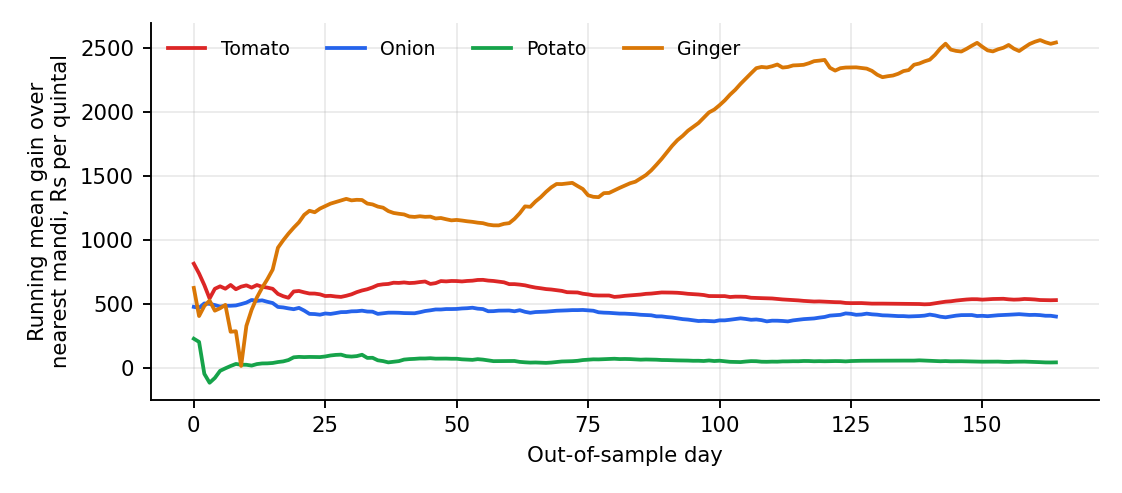
\includegraphics[width=0.82\textwidth]{figures/fig_track.png}
\caption{Running mean gain of the advice over the nearest mandi, by crop, on out-of-sample days.}
\label{fig:track}
\end{figure}

\begin{table}[!t]
\centering
\caption{Floor violation (target 10\%) under three evaluations}
\label{tab:floorcmp}
\gentable{tab_floorcmp}
\end{table}

\subsection{Silence tax}

Over \SilenceMandis{} tomato mandis, a trip loses Rs~\SilenceMean{} per quintal on average to unexpected silence. The costliest is \SilenceTopName{}, at Rs~\SilenceTopLoss{} per quintal (\SilenceTopPct\% of its price): it reported on 44\% of days and is silent on Sundays, on top of which it is unpredictably silent on other days (Table~\ref{tab:silence}). Chikkaballapur reported on none of the Thursdays in the last year (\ThursdayChik\% silent), so it is treated as closed that day, and a farmer is warned not to take a Thursday load there. A tax of Rs~0 for cheap mandis such as Kolar does not mean they are reliable; it means their usual price is below the fallback, so silence costs no money on price. Figure~\ref{fig:silence} shows every mandi by weekday. A day with no price may be a closed mandi or a missed upload, which the portal does not distinguish.

\begin{table}[!t]
\centering
\caption{Silence tax per mandi, tomato, last 365 days}
\label{tab:silence}
\gentable{tab_silence}
\end{table}

\begin{figure}[!t]
\centering
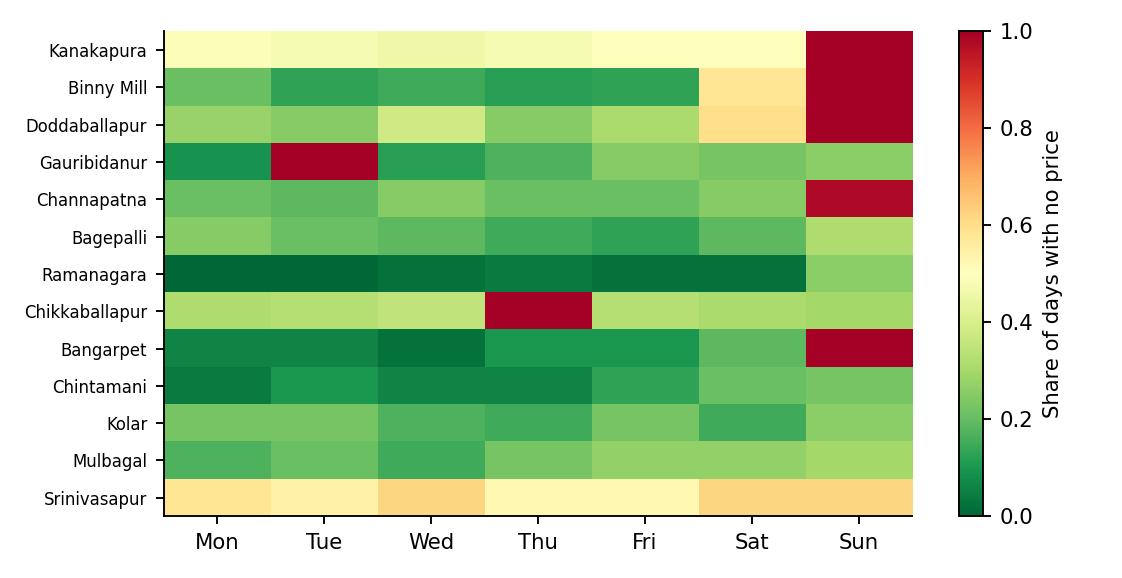
\includegraphics[width=0.85\textwidth]{figures/fig_silence.png}
\caption{Share of days on which each tomato mandi reported no price, by weekday. Red columns are days a mandi is effectively closed.}
\label{fig:silence}
\end{figure}

\subsection{What happens when many farmers follow the advice}

Table~\ref{tab:crowd} and Figure~\ref{fig:crowd} show the effect for 10 quintals per farmer, tomato, Kolar farmers. A single farmer nets Rs~\CrowdAlone{} per quintal. If 200 farmers (2,000 quintals) all follow the advice, the best yard, which usually receives about \CrowdYard{} quintals a day, sees its price fall by \CrowdDrop\% and each farmer nets Rs~\CrowdBest{}, which is no better than everyone going to the nearest mandi (Rs~\CrowdNearest{}). A coordinated split, telling farmers different actions with the stated probabilities, nets Rs~\CrowdCoord{}: Rs~\CrowdGain{} per quintal more, Rs~\CrowdTotal{} for the group. As the crowd grows to 2,000 farmers every policy deteriorates and coordination matters more. Table~\ref{tab:crowdb} shows how much of this depends on the assumed price flexibility $b$: with $b=0$ the crowd costs nothing and all policies are equal, and the conclusion strengthens as $b$ rises. This is a scenario, not a measurement: the flexibility is an association in past data and the real response to a crowd of advised farmers has not been observed.

\begin{table}[!t]
\centering
\caption{Net revenue per quintal (Rs) under four policies as the crowd grows, tomato, Kolar farmers, 10 quintals each}
\label{tab:crowd}
\gentable{tab_crowd}
\end{table}

\begin{figure}[!t]
\centering
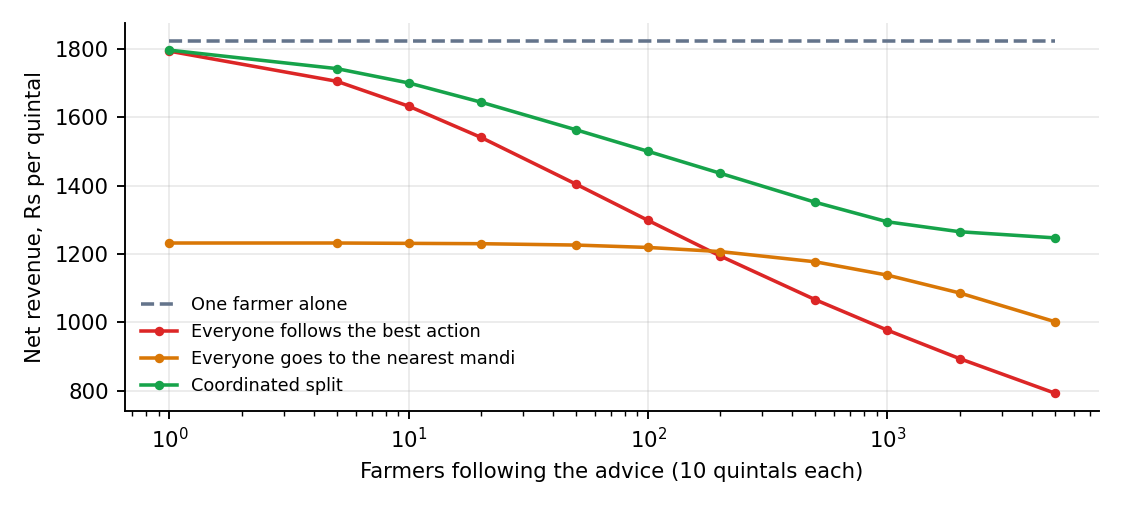
\includegraphics[width=0.82\textwidth]{figures/fig_crowd.png}
\caption{Net revenue per quintal against the number of farmers following the advice.}
\label{fig:crowd}
\end{figure}

\begin{table}[!t]
\centering
\caption{Sensitivity to the price flexibility $b$, 200 farmers}
\label{tab:crowdb}
\gentable{tab_crowdb}
\end{table}

\section{Validation}
\label{sec:validation}

\subsection{Leakage audit of decompose-then-forecast models}
\label{sec:leakage}

Table~\ref{tab:leak} compares the published protocol, in which the series is decomposed once over its whole length, with a causal protocol that decomposes only data available at each forecast origin, for tomato. The published protocol reports skill against the random walk of +27\% to +62\%. Under the causal protocol the same models score between $-15\%$ and $-1\%$, no better than the raw series ($-14\%$ to $-1.5\%$). The difference, 30 to 71 points with intervals that exclude zero, is look-ahead leakage: STL and VMD are two-sided smoothers, so the component at day $t$ already contains the prices that follow it. A zero-shot foundation model was also worse than no change (skill \ChronosOne{}\% at one day and \ChronosSeven{}\% at seven days), so no model in this comparison beat the random walk on the daily tomato series. We did not audit the specific published studies; the claim is about the protocol they describe.

\begin{table}[!t]
\centering
\caption{Forecast skill against the random walk (\%), tomato. Published: series decomposed once over its whole length; causal: decomposed only on data available at each origin; raw: no decomposition. Gap: published minus causal, in percentage points}
\label{tab:leak}
\gentable{tab_leak}
\end{table}

\begin{figure}[!t]
\centering
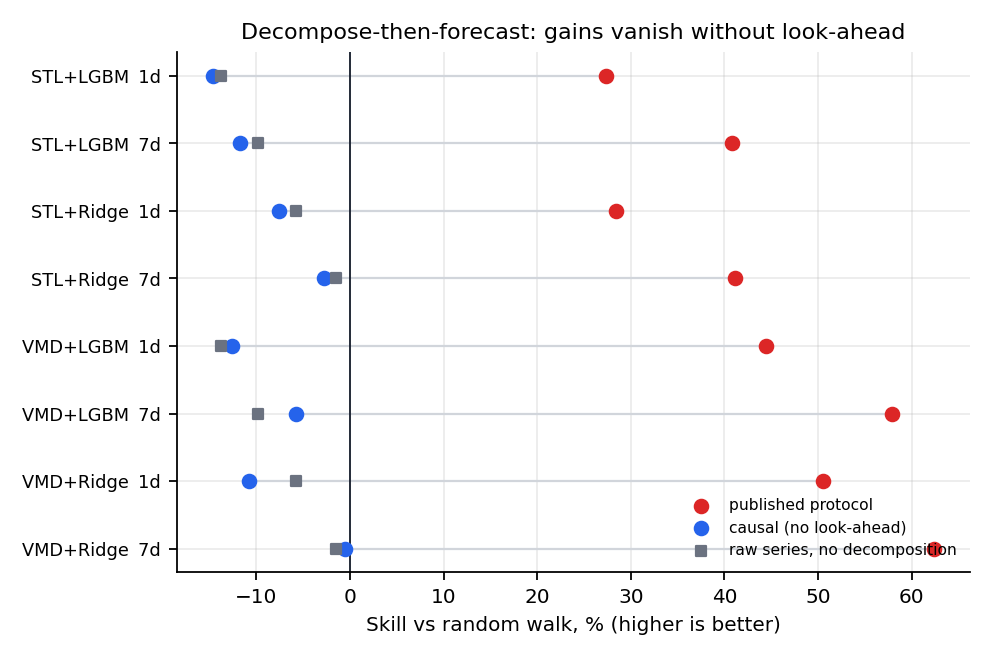
\includegraphics[width=0.85\textwidth,height=7.2cm,keepaspectratio]{figures/fig_leakage.png}
\caption{Skill of decompose-then-forecast models under the published and causal protocols.}
\label{fig:leak}
\end{figure}

\subsection{Sensitivity to assumptions}

Transport cost, spoilage and silent-market discount are assumptions, so ten settings per crop were swept at evaluation time, while models stayed trained under the defaults (Table~\ref{tab:sens}). Across the sweep, models trained on realised outcomes closed 9--36\% of the gap to the oracle relative to the highest price yesterday, while models trained on observed prices stayed between $-8\%$ and $+2\%$. The conclusion in Section~\ref{sec:effects} therefore does not depend on the default economics.

\begin{table}[!t]
\centering
\caption{Range of share of oracle gap closed (relative to the highest price yesterday) across the sensitivity sweep}
\label{tab:sens}
\gentable{tab_sens}
\end{table}

\subsection{Supply shocks}

An event study asked whether large arrival shocks move prices over 3, 7 and 14 days, with placebo circular shifts, minimum detectable effects and Holm correction across \ShockTested{} crop-horizon tests. None was robust (\ShockRobust{}); \ShockSuggestive{} were suggestive (Table~\ref{tab:shock}), and for each the detectable effect was comparable to or larger than the estimate, so power was marginal. These are reported as null results: the data do not support supply-shock trading advice, and the application labels the evidence tier on its shock page.

\begin{table}[!t]
\centering
\caption{Suggestive supply-shock effects, in percent (none survived Holm correction). MDE: minimum detectable effect; placebo $p$ from circular shifts of the shock series}
\label{tab:shock}
\gentable{tab_shock}
\end{table}

\begin{figure}[!t]
\centering
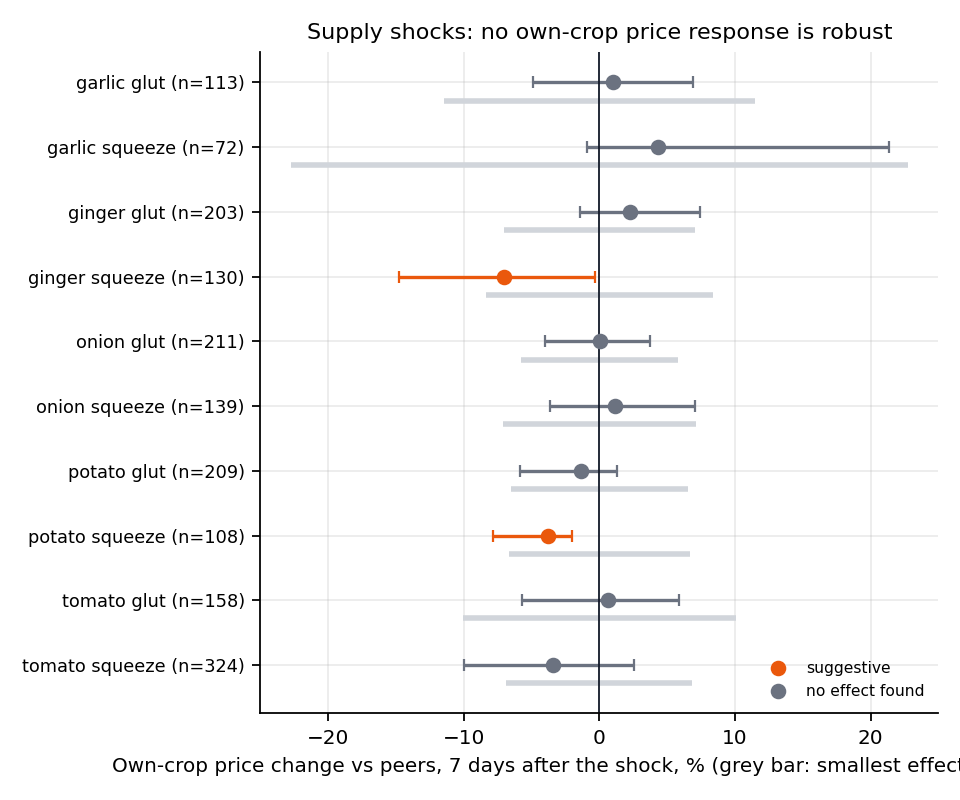
\includegraphics[width=0.85\textwidth,height=7.2cm,keepaspectratio]{figures/fig_shock_effects.png}
\caption{Estimated price effects of arrival shocks with intervals and minimum detectable effects.}
\label{fig:shock}
\end{figure}

\subsection{Cross-commodity spillover}
\label{sec:spill-results}

The engine was run on a weekly panel of five crops over \SpillPeriods{} weeks. Removing the first common factor took out \SpillVar{}\% of the variance of weekly returns, which is the part of co-movement that would otherwise have been read as transmission. Detecting shock episodes from the supply-regime labels then gave \SpillTotalEpisodes{} episodes in every source crop and direction (Table~\ref{tab:spill}), against an evidence floor of eight. All \SpillInsufficient{} of the 40 edges were therefore published as insufficient evidence, no effect size was reported, and the holdout sign-agreement check had no pair to compare (\SpillHoldPairs{} pairs). The engine did what it was built to do, which is to withhold a number it cannot support; the result is that this thesis \emph{does not} show that a shortage in one crop moves another. The AI brief consequently states that spillover evidence is not available rather than citing a link.

\begin{table}[!t]
\centering
\caption{Shock episodes detected per source crop on the weekly panel (floor: 8 episodes)}
\label{tab:spill}
\gentable{tab_spill}
\end{table}

\noindent Zero episodes in all ten source and direction cells is itself a finding about the pipeline, not only about the market: the episode detector depends on supply-regime labels that the preprocessing stage derives from arrivals, and on the real panel no weekly series was labelled squeeze or glut. Whether that reflects a genuinely calm market over 2021--2026, an over-strict labelling threshold, or a labelling stage that is not fed from the real panel has not been resolved, and is listed under future work. The supply-shock event study above, which defines shocks directly from arrivals, did find suggestive same-crop effects, so the data are not shock-free.

\subsection{Decision intelligence and the language layer}
\label{sec:llm-results}

The decision-intelligence service of Section~\ref{sec:intel-method} was tested at two levels. At the code level, 30 unit tests of the brief schema, the evidence bundle, the grounding verifier and the service pass. An invented price is caught; an unknown evidence key is caught; a figure copied from the evidence, or rounded in prose, is accepted; dates and small integers are not treated as claims; a recommended hold is overridden when spoilage outruns the expected gain, in line with the farmer tool's rule; a failing provider falls back to the deterministic one without raising; and withheld spillover evidence is explained in the bundle instead of being shown as zero. At the language level, the writer and judge were evaluated as follows. No study of whether briefs change decisions was done, and the grounding check establishes that figures are traceable to evidence, not that the recommendation is correct; the recommendation itself is the engine's, whose accuracy is reported in Section~\ref{sec:performance-evaluation}.

\LlmExplanations{} explanations (\LlmSentences{} sentences) were generated in English, Kannada and Hindi and judged by an independent model (Table~\ref{tab:llm}). No sentence was rejected by the number validator. The judge rejected 2 of 40 English, 9 of 40 Kannada and 7 of 40 Hindi sentences, which fall back to the original text; the share kept from the model was lower in Kannada and Hindi (0.62--0.88 and 0.68--0.91) than in English (0.83--0.99). To test whether the judge could be trusted, \JudgeBad{} deliberately corrupted explanations and \JudgeGood{} faithful ones were presented: the judge caught \JudgeCaught{} of \JudgeBad{} and wrongly rejected \JudgeFalse{} of \JudgeGood{}. The sample is small, so this shows the judge is not trivially blind rather than that it is reliable. Median latency was \LlmLatency{} seconds per explanation.

\begin{table}[!t]
\centering
\caption{Explanation evaluation by language}
\label{tab:llm}
\gentable{tab_llm}
\end{table}

\subsection{Morning digest}

The digest was tested at two levels. Eight unit tests, using a fake Telegram client with no network, check that every price carries its date and the age of the data, that advice appears only for crops with strong evidence, that the Kannada digest uses Kannada labels, that free-text queries find a crop and a place in the three languages, that onboarding subscribes a farmer and sends the first message, that a farmer who selects no crop is refused, and that unsubscribing removes them from the broadcast. The bot then ran against the real Telegram service: one real account (a team member's) subscribed through the buttons and received two welcome digests, both recorded as sent in the delivery log, and Figure~\ref{fig:digest} shows the message text for tomato and potato at Kolar. A pilot with farmers and a live price feed were not part of this work, so no claim is made about use or effect, and the digest is only as fresh as the last data load (3 days old on 29 October 2026), which it states in its second line.

\begin{figure}[!t]
\centering
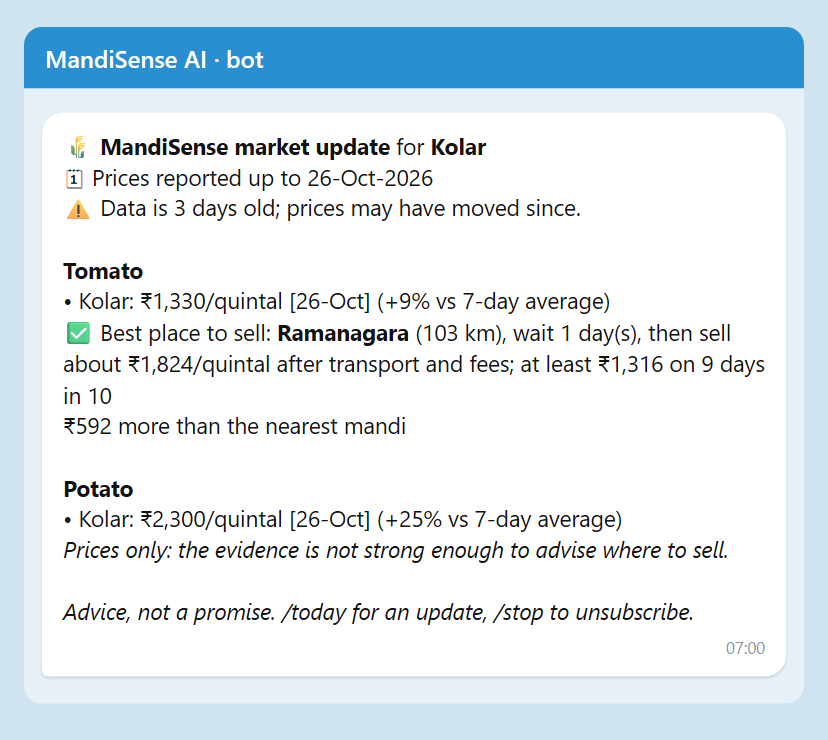
\includegraphics[width=0.34\textwidth]{figures/ins_digest.png}
\caption{The digest message for tomato and potato at Kolar, as sent by the bot (the message text rendered in a chat bubble; the date shown on the first line is the date of the data).}
\label{fig:digest}
\end{figure}

\section{Comparative Analysis}
\label{sec:comparative-analysis}

No published study evaluates mandi choice by regret on real reporting-gap data, so decision results are compared with the heuristics a farmer would plausibly use (Table~\ref{tab:decision}) and with the standard predict-then-optimise baseline, rather than with another paper's numbers. On forecasting, the comparison with published practice is the leakage audit (Table~\ref{tab:leak}) and the foundation-model baseline, and in both the headline accuracy reported for decomposition hybrids was not reproduced under causal evaluation. The contrast between approaches is summarised in Table~\ref{tab:comparative}.

\begin{table}[!t]
\centering
\caption{Comparison of approaches on what they were shown to achieve here}
\label{tab:comparative}
\small
\begin{tabular}{|p{4.3cm}|p{5.2cm}|p{4.9cm}|}
\hline
\textbf{Approach} & \textbf{Result in this study} & \textbf{Qualification} \\ \hline
Nearest mandi, sell today & Lowest revenue in all crops & Common farmer practice \\ \hline
Highest price yesterday & Strong heuristic; 0.17--0.69 of gap closed & Hard to beat in potato \\ \hline
Boosting on observed prices & Indistinguishable from the heuristic & Never sees a silent market \\ \hline
Boosting on realised outcomes & Best or tied-best in all crops & Cost-aware, silence-aware \\ \hline
Neural SPO+ & Tied with boosting & No loss effect found \\ \hline
STL/VMD hybrids, published protocol & +27 to +62\% skill & Disappears causally \\ \hline
Foundation model (zero-shot) & Worse than no change & Daily tomato series \\ \hline
\end{tabular}
\end{table}

\section{Model Optimisation and Innovation}
\label{sec:model-optimization}

\noindent\textbf{What was tried.} Hyper-parameters were tuned with Optuna on a native criterion per method; tuning the most complete model on forecast loss instead of decision regret made no reliable difference. Table~\ref{tab:ablation} lists the four ablations. The reporting head, which models whether a market will report, made decisions \emph{worse} for tomato (Rs~+23 regret, $p=0.012$). Network-silence features, which carry information on whether neighbouring markets are silent, did not reliably help (Rs~$-12$, $p=0.70$). Both were pre-specified hypotheses that failed, and they are reported as such.

\begin{table}[!t]
\centering
\caption{Ablations: change in regret (negative is better) with Holm-adjusted $p$}
\label{tab:ablation}
\gentable{tab_ablation}
\end{table}

\noindent\textbf{What is new.} The contribution that survives testing is the combination: (i) training on realised, silence-aware revenue, which is simple and gave the one robust gain; (ii) floors calibrated online with delayed feedback, which held their nominal level; and (iii) a leak-free evaluation that exposed the inflation in decomposition hybrids. Equation~\ref{eq:aci} is standard adaptive conformal inference~\cite{gibbs2021}; the novelty lies in applying it to selected actions whose outcome resolves $k$ days later.

\noindent\textbf{Limitations of the results.} One region, one source and 5.8 years; revenue parameters are scenarios; ``did not report'' is treated as ``no sale''; and the study is offline, so the effect of farmers acting on the advice is unmeasured.\par

\chapter{Conclusion and Future Discussion}
\label{ch:concl}

\section{Conclusion}
\label{sec:conclusion}

MandiSense AI was built to answer one question for a farmer in the Bengaluru--Kolar belt: where, and when, to sell. Real Agmarknet records (\NhistoryRows{} rows, \DataFrom{} to \DataTo{}) were arranged into a panel of \NpanelRows{} mandi-days, and a market-choice model was trained on the revenue a farmer would actually have received, with transport, shrinkage and silent markets included.

Against the objectives of Section~\ref{sec:objectives}: the panel was built with every exclusion recorded (objective 1, met). Net revenue was formulated and models were scored on 511 to 963 held-out days per crop (objective 2, met). Realised-revenue labels improved decisions in all four crops by Rs~87 to 157 per quintal (Table~\ref{tab:effect}), while the decision-focused loss added no reliable gain (objective 3, met as a test; the second hypothesis was not supported). Adaptive floors held their level in tomato and ginger and were conservative in onion and potato (objective 4, met for two of four crops). The system was delivered as a service and a trilingual application with 650 passing tests and a reproducible pipeline (objective 5, met; public deployment unverified). The audit showed that the large skill reported by decompose-then-forecast models disappears under causal evaluation (objective 6, met). The decision-intelligence service was built with a grounding verifier, a deterministic fallback and 30 passing tests, and the explanation layer kept 0.83 to 0.99 of English sentences and 0.62 to 0.91 of Kannada and Hindi sentences after an independent judge that caught nine of nine corrupted rewrites (objective 7, met for the service and its verifier; not evaluated for the effect of briefs on decisions). The spillover engine was built and run on all 40 edges but published none, because no shock episode reached the evidence floor (objective 8, met as engineering; no transmission result is claimed). The five insight features were built and tested: the breakdown adds up exactly, the advice survives a transport cost over four times the default and changes at 5\% spoilage a day, the replay shows the advice beating the nearest mandi on 63 to 93\% of days with the floor holding on 84 to 92\%, the silence tax puts a figure on unreliable mandis, and 200 farmers all following the best advice cut that mandi's price by 32\% (objective 9, met; the crowd effect is a scenario). A Telegram bot that builds and sends a dated digest in three languages, with a delivery log, was built, unit-tested against a fake client and delivered to one real account with the sends logged (objective 10, met as built and tested; no farmer pilot was run).

In the daily back-test, the served advice earned Rs~\EngineTomatoGain{} per quintal more than the strongest heuristic for tomato, a 62\% share of the gap to the oracle, and was not distinguishable from it for potato. Two further ideas, the specialist council and the supply-shock study, were evaluated honestly and were not promoted. The project's contribution is therefore a tested decision aid with stated limits.

\section{Key Learnings}
\label{sec:key-learnings}

\begin{itemize}
    \item \textbf{Data provenance comes first.} The first dataset in the repository was synthetic; discovering it late cost weeks. Every dataset now carries a load report and an integrity check between independent exports.
    \item \textbf{Evaluation design decides conclusions.} Walk-forward splits with gaps, block bootstrap and multiple-comparison control turned several apparent gains into null results, and exposed the leak in decomposition hybrids.
    \item \textbf{Report negative results.} The decision-focused loss, the reporting head, silence features, the council and the shock study did not help; recording them saved readers from believing otherwise.
    \item \textbf{Make claims testable.} Writing a results generator, so that no number in the report is typed by hand, removed a class of transcription errors.
    \item \textbf{Dependencies need pins.} An unpinned upgrade broke the data stack; a lock file and a fresh-clone check now guard it.
    \item \textbf{Make advice inspectable.} Showing the arithmetic, the break-even cost and the record on unseen days exposed that the floors held on 84 to 92\% of replayed days against the 90\% aimed for, a weakness the headline back-test had hidden.
    \item \textbf{Teamwork.} Splitting work into data, application and verification packages worked on paper; the commit history shows the work concentrated in one member's repository account, a coordination weakness the team recognises (Section~\ref{sec:ram}).
\end{itemize}

\section{Mapping to a Complex Engineering Problem}
\label{sec:cep}

\begin{table}[!t]
\centering
\caption{Attributes of a complex engineering problem and how this project exhibits them}
\label{tab:cep}
\small
\begin{tabular}{|p{3.6cm}|p{8.2cm}|l|}
\hline
\textbf{Attribute} & \textbf{Evidence in this project} & \textbf{Section} \\ \hline
Depth of knowledge & Statistics of forecasting, conformal inference, optimisation, web engineering & \ref{sec:proposed} \\ \hline
Conflicting requirements & Accuracy against interpretability; farmer simplicity against statistical caveats; coverage against floor tightness & \ref{sec:floor-results} \\ \hline
Depth of analysis & No ready formula: revenue, floor and evaluation protocol were derived and tested & \ref{sec:formulation} \\ \hline
Familiarity of issues & Reporting gaps and delayed feedback are not covered by standard forecasting practice & \ref{sec:related-forecast} \\ \hline
Extent of codes and standards & Time-ordered evaluation practice; API typing; data-source terms of the Agmarknet portal & \ref{sec:setup} \\ \hline
Stakeholder involvement & Farmers and traders as users, the guide as reviewer; survey instrument prepared, field responses not collected & Appendix~\ref{appendix:survey} \\ \hline
Interdependence & Data, models, service, language layer and interface depend on one another & \ref{sec:architecture} \\ \hline
\end{tabular}
\end{table}

\section{Limitations and Future Work}
\label{sec:future-work}

\noindent\textbf{Limitations.} One region, one data source and 5.8 years of history; revenue parameters are scenarios; the study is offline and no farmer acted on the advice; garlic is not covered; the language layer is weaker in Kannada and Hindi than in English, and the judge was validated on only nine corrupted and three faithful English sentences; briefs were verified for traceability of figures, not tested with users; the spillover engine found no episodes and so no transmission; the crowd effect rests on an assumed price flexibility; the replayed floors held on 84 to 92\% of days against 90\% aimed for; the digest has not been piloted with farmers and has no live feed; the public deployment has not been verified.

\noindent\textbf{Future work, in priority order.}
\begin{enumerate}
    \item \emph{Field pilot.} Run the survey (Appendix~\ref{appendix:survey}) and a small trial with farmers, to measure whether advice changes decisions and revenue. This is the largest gap.
    \item \emph{Estimate the economics.} Replace assumed transport, spoilage and silent-market parameters with measured values, which Section~\ref{sec:performance-evaluation} showed to be influential but not decisive.
    \item \emph{Understand silence.} Collect reasons for non-reporting from mandi officials, to test the assumption that a silent day means no sale.
    \item \emph{Verify deployment} and add monitoring of floor violations in production, which is the check that matters once advice is live.
    \item \emph{Diagnose the spillover pipeline.} Establish why the weekly panel yields no squeeze or glut episodes (market calm, labelling threshold, or labelling stage not fed from the real panel), define episodes directly from arrivals as the shock study does, and rerun the 40 edges.
    \item \emph{Evaluate briefs with users.} Test whether grounded briefs change decisions or confidence, and extend the judge's validation to Kannada and Hindi with native-speaker review.
    \item \emph{Widen coverage} to more districts and crops, and larger lots with price impact.
\end{enumerate}

\section{Sustainable Development Goals}
\label{sec:sdgs-achieved}

The project addresses three goals. Each connection below separates what the evidence supports from what remains a potential.

\noindent\textbf{SDG 2, Zero Hunger (target 2.3).} Target 2.3 aims to raise the incomes of small-scale food producers, including through access to markets and information. The system gives a smallholder the market-comparison advice that traders already have. Evidence: in the daily back-test the advice earned Rs~60 to 202 per quintal more than the strongest simple rule in three of four crops, and Rs~69 to 1,595 more than selling at the nearest mandi. These are offline figures; the real income effect is not measured. The morning digest puts the same information on a free messaging channel in three languages; whether farmers use it is untested.

\noindent\textbf{SDG 1, No Poverty (target 1.1/1.4 on access to economic resources and services).} Volatile prices and lack of information keep the poorest sellers poor; a free, trilingual tool lowers the barrier. Evidence is indirect: the interface is in Kannada, Hindi and English, and works for small lots. No poverty outcome was measured.

\noindent\textbf{SDG 12, Responsible Consumption and Production (target 12.3).} Target 12.3 calls for reducing food loss along production and supply chains. Spoilage is built into the revenue model, so advice avoids waiting where shrinkage costs more than the expected price gain. The loss avoided is not measured in kilograms and is a potential rather than a result.

\noindent\textbf{SDG 9, Industry, Innovation and Infrastructure (target 9.c).} The system uses a public data feed to widen access to information technology; the pipeline, tests and open documentation are reusable. This is an engineering contribution rather than a measured impact.

\vspace{0.3cm}
\noindent The evidence is strongest where the numbers are from held-out data (SDG 2.3) and weakest where the link is plausible but unmeasured (SDG 1, 12.3). We make no claim beyond that.


\appendix
\renewcommand{\chaptername}{Appendix}
\chapter*{Appendices}
\addcontentsline{toc}{chapter}{Appendices}

\noindent This part holds material too detailed for the chapters. Each appendix is referred to in the text: Appendix~A from Chapter~\ref{ch:impl}, Appendix~B from Section~\ref{sec:cep} and Section~\ref{sec:future-work}, Appendix~C from Chapter~\ref{ch:results}, Appendix~D from Section~\ref{sec:dataset}, Appendix~E from Section~\ref{sec:sdgs-achieved}, and Appendix~F from the front matter.

\chapter{Sample Code Used in the Core Modules}
\label{appendix:code}

The listings are read directly from the source files of the repository, so they cannot drift from the code that produced the results.

\section{Revenue of every action (net of transport, spoilage and fee)}
\begin{lstlisting}[language=Python, caption={\texttt{mandisense\_ai/market\_choice/econ.py}: revenue of every action}]
def revenue_from_prices(price_mk, gate_price, dist_km, e):
    """price_mk (..., M, N_HOLD), gate_price (...), dist_km (M,) -> revenue of every action (..., A)."""
    rev = price_mk * hold_discount(e) - trip_cost(dist_km, e)[:, None]
    flat = rev.reshape(*rev.shape[:-2], -1)
    gate = (e.farmgate_factor * gate_price)[..., None]
    return np.concatenate([flat, gate], axis=-1)
\end{lstlisting}

\section{SPO+ loss and regret}
\lstinputlisting[language=Python, firstline=20, lastline=40, caption={\texttt{research/gfmc/models/losses.py}: SPO+ loss and realised regret}]{../research/gfmc/models/losses.py}

\section{Conformal quantile}
\lstinputlisting[language=Python, firstline=27, lastline=35, caption={\texttt{mandisense\_ai/market\_choice/conformal.py}: finite-sample conformal quantile}]{../mandisense_ai/market_choice/conformal.py}

\section{Online floor with delayed feedback}
\lstinputlisting[language=Python, firstline=64, lastline=88, caption={\texttt{mandisense\_ai/market\_choice/conformal.py}: online floor loop (excerpt)}]{../mandisense_ai/market_choice/conformal.py}

\section{Grounding verification of a decision brief}
\lstinputlisting[language=Python, firstline=90, lastline=127, caption={\texttt{mandisense\_ai/intelligence/grounding.py}: figures, evidence keys and market names in a brief are checked against the evidence}]{../mandisense_ai/intelligence/grounding.py}

\section{Crowd simulation: price impact and a coordinated split}
\lstinputlisting[language=Python, caption={\texttt{mandisense\_ai/market\_choice/insights.py}: yard price falls with the quantity received; greedy split on marginal revenue}]{generated/code_crowd.txt}

\section{Digest block for one crop}
\lstinputlisting[language=Python, caption={\texttt{mandisense\_ai/notify/digest.py}: one crop's lines of the morning digest (non-ASCII characters shown as ASCII)}]{generated/code_digest.txt}

\chapter{Survey Form}
\label{appendix:survey}

\noindent\textbf{Status.} This instrument was prepared to learn how farmers and traders decide when and where to sell, and what form of advice they would use. No response data are reported in this thesis, and nothing in Chapters~\ref{ch:method}--\ref{ch:results} depends on it.

\noindent\textbf{Objective.} Identify difficulties in deciding when and where to sell; understand current decision habits; assess awareness of data tools; and find the preferred form of advice.

\begin{enumerate}
    \item What is your primary role? (Farmer / Trader / Aggregator / Other)
    \item How do you currently decide when to sell your produce? (Past experience / Mandi price trends / Advice from others / Other)
    \item Do you face uncertainty in predicting future prices? (Yes / No)
    \item Which factors influence your selling decision most? (Market arrivals / Seasonal demand / Weather / Government policy / Other)
    \item How many mandis can you reach in a day, and what does the transport cost per trip?
    \item Have you travelled to a mandi and found it closed or without trade? How often? (Never / Sometimes / Often)
    \item Would you use a system that gives: price predictions; a recommendation of where and when to sell; an explanation of the recommendation? (Tick all)
    \item Would a stated minimum expected revenue make you more willing to follow a recommendation? (Yes / No / Unsure)
    \item Preferred language: Kannada / Hindi / English.
    \item Preferred platform: Mobile application / Web dashboard / SMS alerts / Telegram or WhatsApp message.
    \item Would a message every morning with the latest reported prices and the best place to sell be useful, and at what hour? (Yes / No; hour)
\end{enumerate}

\chapter{Detailed Evaluation Tables}
\label{appendix:metrics}

The evaluation in this work is of decisions and regression, not classification, so a confusion matrix does not apply. The matching detail is the per-fold revenue of the main methods, which shows whether the result is carried by one period. Table~\ref{tab:perfold} gives it for tomato across the five outer test blocks, and Table~\ref{tab:ablation} in Chapter~\ref{ch:results} lists the ablations.

\begin{table}[!t]
\centering
\caption{Mean realised revenue (Rs per quintal) by outer fold, tomato}
\label{tab:perfold}
\gentable{tab_perfold}
\end{table}

\noindent The ordering of the realised-outcome model against the heuristics is not the same in every fold, so the pooled gain should be read with its interval (Table~\ref{tab:decision}) and not as a constant.

\section{Insight features: further tables}
Table~\ref{tab:c-crowdb} gives the crowd simulation under five values of the price flexibility, and Table~\ref{tab:c-whatif} the what-if scenarios, both referred to from Section~\ref{sec:insight-results}.

\begin{table}[!t]
\centering
\caption{Crowd simulation, 200 farmers, by price flexibility}
\label{tab:c-crowdb}
\gentable{tab_crowdb}
\end{table}

\begin{table}[!t]
\centering
\caption{What-if scenarios, tomato at Kolar}
\label{tab:c-whatif}
\gentable{tab_whatif}
\end{table}

\chapter{Dataset Description}
\label{appendix:dataset}

\section{D.1 Source and access}
Daily price and arrival records of the Agricultural Marketing Information Network (Agmarknet) of the Government of India~\cite{agmarknet}, exported from the public portal by the project team: the ``All Type of Report (All Grades)'' history export (2021-01-01 to \DataTo) for Karnataka, and the ``Daily Price Arrival Report'' from 2025-11-07. The data are public; no personal data are involved.

\section{D.2 Files and volumes}
\begin{table}[!t]
\centering
\caption{Dataset volumes}
\label{tab:d-volumes}
\small
\begin{tabular}{|l|l|r|}
\hline
\textbf{Artefact} & \textbf{Content} & \textbf{Rows} \\ \hline
History export, cleaned & Market-crop-day modal price and arrivals & \NhistoryRows \\ \hline
Market panel & Mandi-days for five crops, 16 mandis & \NpanelRows \\ \hline
District observations & District-level observation store with quality flags & \NdistrictRows \\ \hline
Mandi prices & Daily report records with minimum and maximum & \NmandiRows \\ \hline
\end{tabular}
\end{table}

\section{D.3 Schema}
\begin{table}[!t]
\centering
\caption{Fields of the market panel and the observation store}
\label{tab:d-schema}
\small
\begin{tabular}{|l|l|p{7.2cm}|}
\hline
\textbf{Table} & \textbf{Field} & \textbf{Meaning} \\ \hline
Panel & date, crop, mandi\_id & Key; one row per market, crop and day reported \\ \hline
Panel & price & Arrivals-weighted modal price, Rs per quintal \\ \hline
Panel & arrivals & Quantity arrived \\ \hline
Observations & modal\_price, min\_price, max\_price & Daily report prices \\ \hline
Observations & state, district, source & Location and origin of the record \\ \hline
Observations & quality\_score, quality\_flags & Result of the quality checks \\ \hline
\end{tabular}
\end{table}

\section{D.4 Cleaning and exclusions}
The loader drops footer rows, rejects unexpected units, checks key uniqueness, and records rows read, dropped and kept. Where both exports cover a market-day they agree (Pearson $r=0.99996$ over 3,307 tomato market-days). Nothing is imputed into the panel. A market is offered for a decision only if it reported within the previous 14 days; days on which no market reported (27 of 2,125 for tomato) are excluded from training and scoring. A market enters the market-choice study only with at least 700 reported days. Garlic has one such market and is excluded from the study and refused by the application. Synthetic data found in the initial repository were removed.

\section{D.5 Splits}
Five outer walk-forward test blocks (2024-H1, 2024-H2, 2025-H1, 2025-H2, 2026-01 to 2026-10), each trained on earlier data only, with a gap of $K{+}2$ days before every validation or test block. The five blocks give 963 scored days for tomato, 511 for onion, 569 for potato and 776 for ginger.

\section{D.6 Limitations of the data}
One state and one source; modal prices only, not transaction-level data; a silent market day may be a reporting failure and not a closed market (the sensitivity sweep includes a setting that makes silence free); and the history does not include weather, transport costs or farm-gate prices, which are therefore assumptions (Section~\ref{sec:formulation}).

\chapter{Outcome and Goal Mapping}
\label{appendix:mapping}

\noindent\textbf{Note.} The course-outcome statements and the CO--PO matrix are those of the departmental course file for 23DS7PWPP2; they are reproduced here unchanged and are not restated by the authors. What follows is the project's justification of each programme outcome with the section that demonstrates it.

\section{E.1 Programme outcomes demonstrated}

\begin{table}[!t]
\centering
\caption{Programme outcome (PO) justification with evidence in this thesis}
\label{tab:po}
\small
\begin{tabular}{|c|p{5.2cm}|p{7cm}|}
\hline
\textbf{PO} & \textbf{Outcome} & \textbf{Evidence and section} \\ \hline
PO1 & Engineering knowledge & Statistics, optimisation and conformal inference applied to a pricing decision (Sec.~\ref{sec:proposed}) \\ \hline
PO2 & Problem analysis & Reporting gaps, delayed feedback and decision loss identified as the structure of the problem (Sec.~\ref{sec:problem-statement}) \\ \hline
PO3 & Design of solutions & Engines, floors, service and trilingual interface (Sec.~\ref{sec:architecture}, Ch.~\ref{ch:impl}) \\ \hline
PO4 & Investigation & Pre-specified experiments, paired tests and a leakage audit (Sec.~\ref{sec:setup}, Sec.~\ref{sec:validation}) \\ \hline
PO5 & Modern tool usage & Optuna, LightGBM, PyTorch, FastAPI, Next.js, Telegram Bot API, CI (Table~\ref{tab:software-req}) \\ \hline
PO6 & Engineer and society & Advice for smallholders; evidence tiers shown to users (Sec.~\ref{sec:sdgs-achieved}) \\ \hline
PO7 & Environment and sustainability & Spoilage built into advice (SDG 12.3) \\ \hline
PO8 & Ethics & No synthetic data in results; negative results reported; language layer cannot change numbers (Ch.~\ref{ch:results}) \\ \hline
PO9 & Individual and team work & Work-package ownership (Sec.~\ref{sec:ram}) \\ \hline
PO10 & Communication & This thesis; documentation in the repository \\ \hline
PO11 & Project management and finance & WBS, critical path, risk register, cost (Ch.~\ref{ch:plan}) \\ \hline
PO12 & Life-long learning & New methods learned during the project (Sec.~\ref{sec:key-learnings}) \\ \hline
\end{tabular}
\end{table}

\noindent\textbf{Complex-engineering-problem attributes} exhibited: depth of knowledge, conflicting requirements, depth of analysis, familiarity of issues, extent of codes and standards, stakeholder involvement and interdependence (Table~\ref{tab:cep}).

\section{E.2 Sustainable Development Goals}

\begin{table}[!t]
\centering
\caption{SDG targets, evidence, and whether the effect was measured}
\label{tab:sdg}
\small
\begin{tabular}{|l|p{4.2cm}|p{5.4cm}|l|}
\hline
\textbf{SDG / target} & \textbf{Link} & \textbf{Evidence in this thesis} & \textbf{Status} \\ \hline
2 / 2.3 & Income of small-scale producers through market information & Back-test gains of Rs 60 to 202 per quintal over the best simple rule in three crops (Table~\ref{tab:engine}) & Offline, measured \\ \hline
1 / 1.4 & Access to economic services & Free trilingual tool & Not measured \\ \hline
12 / 12.3 & Reduce food loss in supply chains & Spoilage in the revenue model (Eq.~\ref{eq:revenue}) & Potential \\ \hline
9 / 9.c & Access to information technology & Open pipeline built on a public data feed & Engineering \\ \hline
\end{tabular}
\end{table}

\chapter{Similarity Report}
\label{appendix:similarity}

\noindent The thesis is to be checked with the institution's similarity tool (Drillbit) and the report attached here before submission, with the similarity index within the limit set by the department.

\begin{table}[!t]
\centering
\caption{Similarity check record}
\label{tab:similarity}
\small
\begin{tabular}{|l|l|}
\hline
\textbf{Item} & \textbf{Entry} \\ \hline
Tool & Drillbit \\ \hline
Document checked & Final thesis PDF \\ \hline
Similarity index & \hspace{3cm} \% \\ \hline
Departmental limit & \hspace{3cm} \% \\ \hline
Date of check & \hspace{3cm} \\ \hline
Report & Attached on the following pages \\ \hline
\end{tabular}
\end{table}

\IfFileExists{drillbit_report.pdf}{\includepdf[pages=-]{drillbit_report.pdf}}{}


% Generated by report/gen_bibliography.py from verified records; ordered by first citation.
\clearpage
\addcontentsline{toc}{chapter}{Bibliography}
\begingroup\small\setlength{\itemsep}{1pt}\sloppy\urlstyle{same}
\begin{thebibliography}{999}
\bibitem{agmarknet} Directorate of Marketing and Inspection, Govt.\ of India, ``AGMARKNET: Agricultural marketing information network.'' [Online]. Available: https://agmarknet.gov.in
\bibitem{birthal2019} P.~S. Birthal, A.~Negi, and P.~K. Joshi, ``Understanding causes of volatility in onion prices in India,'' \emph{J. Agribusiness Develop. Emerg. Econ.}, vol.~9, no.~3, pp.~255--275, 2019.
\bibitem{jensen2007} R.~Jensen, ``The digital provide: Information (technology), market performance, and welfare in the South Indian fisheries sector,'' \emph{Quart. J. Econ.}, vol.~122, no.~3, pp.~879--924, 2007.
\bibitem{aker2010} J.~C. Aker, ``Information from markets near and far: Mobile phones and agricultural markets in Niger,'' \emph{Amer. Econ. J.: Appl. Econ.}, vol.~2, no.~3, pp.~46--59, 2010.
\bibitem{ray2023} S.~Ray, A.~Lama, P.~Mishra, T.~Biswas, S.~S. Das, and B.~Gurung, ``An ARIMA-LSTM model for predicting volatile agricultural price series with random forest technique,'' \emph{Appl. Soft Comput.}, vol.~149, 2023, Art.\ no.~110939.
\bibitem{sathe2025} A.~M. Sathe, Supraja R., and A.~A. Thomas, ``Enhancing agricultural sustainability: Time series forecasting with ICEEMDAN-VMD-GRU for economic-resilience,'' \emph{Results Eng.}, vol.~27, 2025, Art.\ no.~106423.
\bibitem{celik2025} B.~A. Celik and S.~Celik, ``Hybrid forecasting of agricultural commodity prices: Integrating machine learning, time series, and stochastic simulation models,'' \emph{Borsa Istanbul Rev.}, vol.~25, no.~6, 2025.
\bibitem{wu2026} Wu \emph{et al.}, ``A comprehensive review for agricultural product prices forecasting: Architectural diversity and open challenges,'' \emph{Expert Syst.}, 2026, doi: 10.1111/exsy.70254.
\bibitem{fafchamps2012} M.~Fafchamps and B.~Minten, ``Impact of SMS-Based Agricultural Information on Indian Farmers,'' \emph{World Bank Econ. Rev.}, vol.~26, no.~3, pp.~383--414, 2012.
\bibitem{hyndman2021} R.~J. Hyndman and G.~Athanasopoulos, \emph{Forecasting: Principles and Practice}, 3rd~ed. Melbourne, Australia: OTexts, 2021.
\bibitem{jha2014} G.~K. Jha and K.~Sinha, ``Time-delay neural networks for time series prediction: An application to the monthly wholesale price of oilseeds in India,'' \emph{Neural Comput. Appl.}, vol.~24, pp.~563--571, 2014.
\bibitem{meena2024} K.~Meena and B.~Chaitra, ``A novel framework using deep learning techniques for ragi price prediction in Karnataka,'' \emph{IEEE Access}, vol.~12, pp.~194829--194838, 2024.
\bibitem{avinash2024} G.~Avinash \emph{et al.}, ``Hidden Markov guided deep learning models for forecasting highly volatile agricultural commodity prices,'' \emph{Appl. Soft Comput.}, vol.~158, 2024, Art.\ no.~111557.
\bibitem{sediyono2025} E.~Sediyono \emph{et al.}, ``An integrated framework for multi-commodity agricultural price forecasting and anomaly detection using attention-boosted models,'' \emph{J. Agric. Food Res.}, vol.~22, 2025, Art.\ no.~102021.
\bibitem{mohanty2023} M.~K.~Mohanty, P.~K.~G.~Thakurta, and S.~Kar, ``Agricultural commodity price prediction model: a machine learning framework,'' \emph{Neural Comput. and Applications}, vol.~35, no.~20, pp.~15109--15128, 2023.
\bibitem{exogenous2024} G.~H.~H.~Nayak \emph{et~al.}, ``Exogenous variable driven deep learning models for improved price forecasting of TOP crops in India,'' \emph{Scientific Reports}, vol.~14, no.~1, Art.\ no.~17203, 2024.
\bibitem{crop_ins} D.~Biswal and C.~S.~Bahinipati, ``Farmers' preference for crop-diversification in India: does crop-insurance play a part?,'' \emph{Mitigation and Adaptation Strategies for Global Change}, vol.~30, no.~3, Art.\ no.~17, 2025.
\bibitem{manogna2025} R.~L.~Manogna, V.~Dharmaji, and S.~Sarang, ``A novel hybrid neural network-based volatility forecasting of agricultural commodity prices: empirical evidence from India,'' \emph{J. Big Data}, vol.~12, no.~1, Art.\ no.~85, 2025.
\bibitem{chen2016} T.~Chen and C.~Guestrin, ``XGBoost: A scalable tree boosting system,'' in \emph{Proc. 22nd ACM SIGKDD Int. Conf. Knowl. Discovery Data Mining}, 2016, pp.~785--794.
\bibitem{ke2017} G.~Ke \emph{et al.}, ``LightGBM: A highly efficient gradient boosting decision tree,'' in \emph{Adv. Neural Inf. Process. Syst.}, vol.~30, 2017.
\bibitem{grinsztajn2022} L.~Grinsztajn, E.~Oyallon, and G.~Varoquaux, ``Why do tree-based models still outperform deep learning on typical tabular data?'' in \emph{Adv. Neural Inf. Process. Syst. (Datasets and Benchmarks Track)}, 2022.
\bibitem{ansari2024} A.~F. Ansari \emph{et al.}, ``Chronos: Learning the language of time series,'' \emph{Trans. Mach. Learn. Res.}, 2024, arXiv:2403.07815.
\bibitem{wang2026} L.~Wang and B.~Zhang, ``The promise of time-series foundation models for agricultural forecasting: Evidence from commodity prices,'' arXiv:2601.06371, 2026.
\bibitem{cleveland1990} R.~B. Cleveland, W.~S. Cleveland, J.~E. McRae, and I.~Terpenning, ``STL: A seasonal-trend decomposition procedure based on loess,'' \emph{J. Official Statist.}, vol.~6, no.~1, pp.~3--73, 1990.
\bibitem{dragomiretskiy2014} K.~Dragomiretskiy and D.~Zosso, ``Variational mode decomposition,'' \emph{IEEE Trans. Signal Process.}, vol.~62, no.~3, pp.~531--544, 2014.
\bibitem{jaiswal2025} R.~Jaiswal, G.~K.~Jha, R.~R.~Kumar, and K.~Choudhary, ``STL-LSTM Hybrid Model for Forecasting Seasonal Agricultural Price Series,'' \emph{Ann. Data Sci.}, vol.~13, no.~2, pp.~279--302, 2025.
\bibitem{ceemdan2024} P.~Pandit \emph{et~al.}, ``Hybrid modeling approaches for agricultural commodity prices using CEEMDAN and time delay neural networks,'' \emph{Scientific Reports}, vol.~14, no.~1, Art.\ no.~26639, 2024.
\bibitem{kde2024} D.~Zhang, X.~Zhang, H.~Hu, B.~Zhang, and L.~Ling, ``A hybrid model for point and interval forecasting of agricultural price based on the decomposition-ensemble and KDE,'' \emph{Soft Comput.}, vol.~28, no.~17-18, pp.~10153--10176, 2024.
\bibitem{bergmeir2012} C.~Bergmeir and J.~M. Ben\'{i}tez, ``On the use of cross-validation for time series predictor evaluation,'' \emph{Inf. Sci.}, vol.~191, pp.~192--213, 2012.
\bibitem{cerqueira2020} V.~Cerqueira, L.~Torgo, and I.~Mozeti\v{c}, ``Evaluating time series forecasting models: An empirical study on performance estimation methods,'' \emph{Mach. Learn.}, vol.~109, pp.~1997--2028, 2020.
\bibitem{diebold1995} F.~X. Diebold and R.~S. Mariano, ``Comparing predictive accuracy,'' \emph{J. Bus. Econ. Statist.}, vol.~13, no.~3, pp.~253--263, 1995.
\bibitem{harvey1997} D.~Harvey, S.~Leybourne, and P.~Newbold, ``Testing the equality of prediction mean squared errors,'' \emph{Int. J. Forecasting}, vol.~13, no.~2, pp.~281--291, 1997.
\bibitem{newey1987} W.~K. Newey and K.~D. West, ``A simple, positive semi-definite, heteroskedasticity and autocorrelation consistent covariance matrix,'' \emph{Econometrica}, vol.~55, no.~3, pp.~703--708, 1987.
\bibitem{holm1979} S.~Holm, ``A simple sequentially rejective multiple test procedure,'' \emph{Scand. J. Statist.}, vol.~6, no.~2, pp.~65--70, 1979.
\bibitem{hansen2011} P.~R. Hansen, A.~Lunde, and J.~M. Nason, ``The model confidence set,'' \emph{Econometrica}, vol.~79, no.~2, pp.~453--497, 2011.
\bibitem{kunsch1989} H.~R. K\"{u}nsch, ``The jackknife and the bootstrap for general stationary observations,'' \emph{Ann. Statist.}, vol.~17, no.~3, pp.~1217--1241, 1989.
\bibitem{akiba2019} T.~Akiba, S.~Sano, T.~Yanase, T.~Ohta, and M.~Koyama, ``Optuna: A next-generation hyperparameter optimization framework,'' in \emph{Proc. 25th ACM SIGKDD Int. Conf. Knowl. Discovery Data Mining}, 2019, pp.~2623--2631.
\bibitem{fiszeder2024} A.~Dutta, G.~S.~Uddin, L.~W.~Sheng, D.~Park, and X.~Zhu, ``Volatility dynamics of agricultural futures markets under uncertainties,'' \emph{Energy Econ.}, vol.~136, pp.~107754, 2024.
\bibitem{algirdas2024} M.~Bonato, O.~Cepni, R.~Gupta, and C.~Pierdzioch, ``Financial stress and realized volatility: The case of agricultural commodities,'' \emph{Res. in Int. Business and Finance}, vol.~71, pp.~102442, 2024.
\bibitem{zeng2023} L.~Zeng, L.~Ling, D.~Zhang, and W.~Jiang, ``Optimal forecast combination based on PSO-CS approach for daily agricultural future prices forecasting,'' \emph{Appl. Soft Comput.}, vol.~132, 2023.
\bibitem{tranad2024} H.~Kang and P.~Kang, ``Transformer-based multivariate time series anomaly detection using inter-variable attention mechanism,'' \emph{Knowledge-Based Syst.}, vol.~290, pp.~111507, 2024.
\bibitem{epu2024} L.~Hao and L.~Ki-Seong, ``The impact of economic policy uncertainty on agricultural prices: Evidence from China,'' \emph{Asia and the Global Economy}, vol.~4, no.~2, pp.~100100, 2024.
\bibitem{demand2023} N.~Darapaneni \emph{et al.}, ``Demand and price forecasting using deep learning algorithms,'' in \emph{Multi-Disciplinary Trends in Artificial Intelligence}, ser. Lecture Notes in Computer Science. Cham, Switzerland: Springer, 2023, pp.~735--746.
\bibitem{optimized2023} M.~Sari, S.~Duran, H.~Kutlu, B.~Guloglu, and Z.~Atik, ``Various optimized machine learning techniques to predict agricultural commodity prices,'' \emph{Neural Comput. and Applications}, vol.~36, no.~19, pp.~11439--11459, 2024.
\bibitem{gcn2024} D.~Zhang, X.~Li, L.~Ling, H.~Hu, and R.~Lin, ``Integrated GCN--BiGRU--TPE agricultural product futures prices prediction based on multi-graph construction,'' \emph{Comput. Econ.}, vol.~66, no.~5, pp.~3927--3955, 2025.
\bibitem{cropyield} A.~TK, K.~Vanitha, and R.~S.~Ravi, ``Survey for Agriculture Crop Yield Prediction and Recommendation Based on Deep Ensemble Learning Models,'' in \emph{2024 Int. Conf. on Emerging Res. in Computational Sci. (ICERCS)}, 2024, pp.~1--6.
\bibitem{agtech2024} N.-B.-v.~Le, Y.-S.~Seo, and J.-H.~Huh, ``AgTech: Volatility Prediction for Agricultural Commodity Exchange Trading Applied Deep Learning,'' \emph{IEEE Access}, vol.~12, pp.~153898--153910, 2024.
\bibitem{smartag2024} B.~Ahmed, H.~Shabbir, S.~R.~Naqvi, and L.~Peng, ``Smart Agriculture: Current State, Opportunities, and Challenges,'' \emph{IEEE Access}, vol.~12, pp.~144456--144478, 2024.
\bibitem{smartfarm2025} L.~Thakre, M.~Daware, A.~Mohite, A.~Sakhare, and P.~Khobragade, ``Smart Farming: Enhancing Crop Recommendation and Price Prediction with Advanced Machine Learning,'' in \emph{2025 6th Int. Conf. for Emerging Technol. (INCET)}, 2025, pp.~1--6.
\bibitem{fedxai2025} H.~A.~Tahir, W.~Alayed, and W.~U.~Hassan, ``A Federated Explainable AI Framework for Smart Agriculture: Enhancing Transparency, Efficiency, and Sustainability,'' \emph{IEEE Access}, vol.~13, pp.~97567--97584, 2025.
\bibitem{elmachtoub2022} A.~N. Elmachtoub and P.~Grigas, ``Smart ``predict, then optimize'','' \emph{Manage. Sci.}, vol.~68, no.~1, pp.~9--26, 2022.
\bibitem{mandi2024} J.~Mandi \emph{et al.}, ``Decision-focused learning: Foundations, state of the art, benchmark and future opportunities,'' \emph{J. Artif. Intell. Res.}, vol.~80, pp.~1623--1701, 2024.
\bibitem{zaheer2017} M.~Zaheer, S.~Kottur, S.~Ravanbakhsh, B.~Poczos, R.~Salakhutdinov, and A.~Smola, ``Deep sets,'' in \emph{Adv. Neural Inf. Process. Syst.}, vol.~30, 2017.
\bibitem{huber1964} P.~J. Huber, ``Robust estimation of a location parameter,'' \emph{Ann. Math. Statist.}, vol.~35, no.~1, pp.~73--101, 1964.
\bibitem{vovk2005} V.~Vovk, A.~Gammerman, and G.~Shafer, \emph{Algorithmic Learning in a Random World}. New York, NY, USA: Springer, 2005.
\bibitem{angelopoulos2023} A.~N. Angelopoulos and S.~Bates, ``Conformal prediction: A gentle introduction,'' \emph{Found. Trends Mach. Learn.}, vol.~16, no.~4, pp.~494--591, 2023.
\bibitem{romano2019} Y.~Romano, E.~Patterson, and E.~Cand\`{e}s, ``Conformalized quantile regression,'' in \emph{Adv. Neural Inf. Process. Syst.}, vol.~32, 2019.
\bibitem{gibbs2021} I.~Gibbs and E.~Cand\`{e}s, ``Adaptive conformal inference under distribution shift,'' in \emph{Adv. Neural Inf. Process. Syst.}, vol.~34, 2021.
\bibitem{rubin1976} D.~B. Rubin, ``Inference and missing data,'' \emph{Biometrika}, vol.~63, no.~3, pp.~581--592, 1976.
\bibitem{che2018} Z.~Che, S.~Purushotham, K.~Cho, D.~Sontag, and Y.~Liu, ``Recurrent neural networks for multivariate time series with missing values,'' \emph{Sci. Rep.}, vol.~8, Art.\ no.~6085, 2018.
\bibitem{gptoss2025} OpenAI \emph{et~al.}, ``gpt-oss-120b \& gpt-oss-20b Model Card,'' arXiv preprint arXiv:2508.10925, 2025.
\bibitem{qwen3} A.~Yang \emph{et~al.}, ``Qwen3 Technical Report,'' arXiv preprint arXiv:2505.09388, 2025.
\bibitem{claude3} Anthropic, ``The Claude 3 model family: Opus, Sonnet, Haiku,'' Anthropic, San Francisco, CA, USA, Model Card, Mar.\ 2024. [Online]. Available: https://www.anthropic.com/claude
\end{thebibliography}
\endgroup

\end{document}
